\section{Introduction}
\iftoggle{toclinks}{\gototoc}{} % Turn it on/off in packages.tex, command in macros.tex
\iftoggle{cboxes}{	   				  % Turn it on/off in packages.tex
	\begin{boxeditems}
		\item Outline: establish time-varying risk premia in EMs (C-P regressions), account for credit risk (D-S), model time-varying *term* premia (ATSM, constant volatility), estimation (Guimaraes), analyze results (drivers of credit and term premia). 
		\item Improve the literature review part.
		\item Research questions: How EM bond yields respond to US MP? Does US MP affect expectations of future policy rates in EMs? Did US UMP reduce TP abroad? Is there a risk premium channel from US to EMs? Do ST and LT yields respond differently?
		\item Requirements to answer those questions: decompose EM yields, to adequately estimate TP: take into account credit risk and use surveys, methodology that enables event studies (estimation with daily frequency).
		\item Reference for theoretical explanations of why EM can default \textit{in LC}: small cost to default in LC if already defaulted in FC, if external debt of firms is large don't want to default in FC.
		\item Review cases of actual default. Papers by Reinhart, database BoC-BoE, S\&P annual report on sovereign defaults.
		\item Why doing this is useful/necessary? To improve the conduct of MP in EMEs: appropriately characterizing expectations, TP and credit risk.
		\item Applications: portfolio allocation, MP, risk management.
		\item Check: literature on other topics.
		\item 'The results are assessed against those of advanced economies and highlight the benefits of using synthetic yields and survey data when analyzing the yields of emerging markets.'
	\end{boxeditems}}{}

%No correction for credit risk: Blake et al, ACDM
%International comparisons focused on advanced economies: Dahlquist and Estoft, Wright.
%More issuances in LC: Du and Schreger, Otonello and Perez, Galli.
%Theoretical explanations of credit risk: Du and Schreger, Galli.
%Why it is important: risk management (simulations), portfolio allocation (high term premium), monetary policy transmission (effects on the components of yields).

% Motivation
U.S. monetary policy has worldwide consequences, yet the channels through which it affects the sovereign bond yields of emerging markets are not well understood. Decomposing the yields and analyzing the effects of U.S. monetary policy on the components is a sensible approach. However, traditional decompositions of sovereign yields are not suitable for emerging markets because they rely on the yields being free of credit risk.


\iftoggle{fulldraft}{	% Turn it on/off in packages.tex

The main contribution of this paper is to empirically quantify the transmission channels of U.S. monetary policy to the sovereign yields of emerging markets.
To achieve this, the paper first proposes to decompose the yields into an average expected future short-term interest rate, a term premium and compensation for credit risk, and then asks how U.S. monetary policy transmits to these components. The ability of emerging markets to effectively mitigate any undesired domestic impact relies on understanding those transmission channels. 
%The value of the decomposition, however, goes beyond this particular application, others include the transmission of monetary policy domestically.
%This paper answers the question: how does U.S. monetary policy transmit to the sovereign bond yields of emerging markets? 

Investors holding local currency bonds of emerging markets bear two major risks. First, they bear the risk of not receiving the promised payments.
%Credit risk in sovereign debt differs across emerging and advanced economies. 
In the last decades, emerging markets depend more on local currency debt as a stable source of funding \citep{IMFWB:2020}, but they are prone to default \citep{ReinhartRogoff:2011}.\footnote{ Before 2000, several emerging markets issued bonds at short maturities and in foreign currency. Nowadays, it is more common for them to issue bonds with longer maturities and in local currency. Examples of overt defaults in local currency debt include Barbados (2018), Jamaica (2013, 2010), Nicaragua (2008, 2003), Argentina (2001), Turkey (1999), Russia (1998).} 
Second, investors also bear the risk that inflation erodes the real value of the payments they may receive.  The compensation for this risk is the standard term premium. Therefore, a compensation for credit risk addresses the risk of not receiving the promised payments, whereas the term premium compensates investors for bearing interest rate risk. 
%, even though they have the ability to print their own currency

To account for credit risk, I use synthetic local currency yields, which essentially swap the U.S. yield curve (a risk-free benchmark) into a local currency one. Synthetic yields can be seen as the borrowing rates paid by a hypothetical bond issuer in local currency with no credit risk, and so traditional decompositions can be applied to them. I use a standard affine term structure model augmented with survey data to obtain robust decompositions of the synthetic yields.\footnote{ \cite{Guimaraes:2014} shows that affine term structure models augmented with survey data provide robust decompositions of the U.S. and U.K. (nominal) yield curves.} Such yields have been widely used to study deviations from covered interest parity (CIP) but, instead of concentrating on the CIP deviations, I focus on the synthetic yields themselves.\footnote{ \cite{DuTepperVerdelhan:2018} show that persistent and systematic deviations from CIP reflect a higher regulatory burden for financial intermediaries. \cite{DuImSchreger:2018JIE} argue that CIP deviations reflect a convenience yield in advanced economies, whereas \cite{DuSchreger:2016JoF} show that they capture a local currency credit spread for emerging markets, which is used by \cite{HofmannShimShin:2019} to explain the link between currency appreciations and the compression of the sovereign yield spreads of emerging markets.} To the best of my knowledge, this is the first application of affine terms structure models to synthetic yields. 
%\footnote{ Section \ref{sec:LCYCs} argues that it is reasonable to assume that the U.S. yield curve and the financial instruments used to swap it are free of credit risk.}

This paper decomposes the nominal (or actual) yields of 15 emerging markets from 2000 to 2019 %accounting for the credit risk embedded in them
into three parts. The first two components come from the decomposition of synthetic yields, namely an average expected future short rate and a term premium. The third component is the spread between the nominal and the synthetic yields, which captures the compensation for credit risk in the local currency debt of emerging markets \citep{DuSchreger:2016JoF}.\footnote{ Credit risk here is broadly defined including, for example, (selective) default risk, currency convertibility risk, regulation risk, capital controls, and jurisdiction risk, so compensation for any of these risks is considered as compensation for credit risk even if the country does not default per se.}
This decomposition gives reasonable estimates for the components.
%the estimated components are reasonable. %estimates for the components. 
Across emerging markets, average expected short rates, the term premium and the credit risk compensation in the 10-year nominal yield represent on average 4.3, 2 and 0.9\%, respectively.
Although credit risk is an important component, % of debt issued by those countries, 
the literature on term structures of emerging market yields has not examined it systematically.\footnote{ The analysis of sovereign credit risk traditionally focuses on bonds denominated in foreign currency. For instance, \cite{HilscherNosbusch:2010} report the relevance of domestic factors to explain sovereign credit risk, while \cite{Longstaffetal:2011} document the importance of global factors. \cite{BostanciYilmaz:2020} study the connectedness of the network of sovereign credit default swaps.} By explicitly accounting for credit risk, the second component is a genuine term premium. %clean of credit risk, 
I show that this term premium aligns with the view that it compensates investors for bearing inflation uncertainty \citep{Wright:2011}, which is worth highlighting since inflation in emerging markets is more volatile than in advanced economies \citep{HaKoseOhnsorge:2019}. 
%it has not been accounted for in the literature that decomposes their (nominal) yields.

The characterization of the transmission channels of U.S. monetary policy needs both the three-part yield decomposition and the identification of unanticipated policy decisions by the Fed.
%The estimated components are reasonable. 
%Further, 
%%They also 
%the components reflect %Each component reflects 
%local circumstances; for instance, the decline in the term premium of Eastern European countries shadows that of Eurozone countries. 
%of the countries in the sample
%Although this decomposition helps to characterize the transmission channels of U.S. monetary policy in this paper, it has of course many more applications (e.g. the transmission of monetary policy domestically). 
%Regarding the monetary policy surprises, 
%In addition to decomposing the yields, 
I distinguish between target, forward guidance and asset purchase surprises following the literature \citep{GSS:2005a,Swanson:2018}. 
%to understand the impact of unanticipated policy decisions by the Fed. %not only requires %decomposing the yields but 
%Nevertheless, 
%distinguishing among the different types of monetary policy surprises. I , 
These monetary policy surprises 
are identified using intraday data around Fed's monetary policy announcements. %, which 
This is by now a well-established strategy %in macro-finance 
to overcome endogeneity concerns because it isolates the surprise component of monetary policy decisions.

Three main findings summarize the transmission channels of U.S. monetary policy surprises to emerging market yields.
First, the responses to target, forward guidance and asset purchase surprises are economically significant but sluggish, and amplify over the month following the surprise. This delayed response is consistent with the evidence for the U.S. and other advanced economies, which \cite{BrooksKatzLustig:2019} attribute to a portfolio rebalancing channel and %that translates into 
slow-moving capital. 
Moreover, the effects of forward guidance and asset purchase surprises last longer in emerging market yields than in U.S. yields. Portfolio rebalancing involving emerging market sovereign bonds is thus slower.
%Rebalancing involving emerging market sovereign bonds is thus slower.

Second, monetary policy surprises spill over to all yield components, so that % not only the term premium, and including the compensation for credit risk. Therefore, 
unanticipated Fed policy decisions give rise to a reassessment of policy rate expectations and a repricing of risks in emerging markets. 
Investors expect monetary authorities in those countries to eventually follow the Fed's monetary stance rather than counteract it, given that average expected future short rates decline following target, forward guidance and asset purchase easing surprises.
In addition, Fed's unconventional monetary policies aimed at reducing the U.S. term premium, namely forward guidance and asset purchases, ultimately also decrease the term premia in emerging markets.
Lastly, long-term credit risk compensation increases following target and forward guidance easing surprises, whereas it eventually decreases in response to an asset purchase easing surprise.
%Target easing surprises eventually reduce the average expected future short rates but increase long-term credit risk compensation. Forward guidance easing surprises led to a parallel decline in the term premium before the global financial crisis; since then, they eventually reduce average expected short rates and the term premium but also increase long-term credit risk compensation. Asset purchase easing surprises eventually decrease all three components of the yields. 
Interpreting the effects on the credit risk compensation %for  transmission of these surprises to emerging market yields 
requires one to understand the response of both
%their effects not only on 
(nominal and synthetic) yield curves. %(like in advanced economies) 
%but also on the synthetic one. 
The surprises trigger (slow-moving) capital flows in or out of emerging markets, whose relative influence %they have 
on each curve in turn determines %the effects on 
the response of the yield components. In particular, the surprises alter the opportunity cost of lending to emerging markets in local currency, so investors adjust the compensation they require for credit risk. %The potential 
The fiscal implications for emerging markets of Fed's monetary policies have thus far not been discussed in the literature.

Third, since the global financial crisis, U.S. monetary policy has spilled over to emerging markets through a yield curve channel. %, according to which their monetary autonomy decreases along the yield curve. 
I show that among emerging markets long-term yields are more interconnected than short-term ones. %, which implies that t
The global financial cycle is therefore more relevant at the long end of the curve; equivalently, the monetary autonomy of emerging markets is stronger at the front end of their yield curves. U.S. unconventional monetary policies aimed at influencing long-term yields thus limit the monetary autonomy of emerging markets along their yield curves. These results are consistent with the mechanisms discussed by \cite{Turner:2014}, \cite{Obstfeld:2015}, \cite{Kalemli-Ozcan:2019} and \cite{KolasaWesolowski:2020}.
 %the correlation among long-term yields is higher than among short term ones
 
A growing literature analyzes the spillover effects of U.S. monetary policy to the local currency sovereign bond yields of emerging markets. \cite{HausmanWongswan:2011} report significant spillovers, %to local currency bond yields, 
while \cite{BowmanLondonoSapriza:2015} compare the effects of 
%distinguish between spillovers from 
conventional and unconventional monetary policies. The present paper is nonetheless more closely related to the work of \cite{CurcuruKaminLiRodriguez:2018}, \cite{ACDM:2019} and \cite{Albaglietal:2019}, who decompose the yields to analyze the transmission channels of such spillovers, but it differs in a number of dimensions. Most importantly, this paper explicitly accounts for the credit risk embedded in emerging market yields, and analyzes the effects of different types of monetary policy surprises identified with intraday data.\footnote{\cite{RogersScottiWright:2014} and \cite{RogersScottiWright:2018} analyze the spillovers on bond yields using surprises identified with intraday data but they focus on advanced economies. \cite{GilchristYueZakrajsek:2019} study the effects for advanced and emerging countries but for debt denominated in foreign currency.}

The rest of the paper proceeds as follows. 
Section \ref{sec:LCYCs} explains how to construct the local currency yield curves. Section \ref{sec:Methodology} presents the affine term structure model used to decompose the yields.
Section \ref{sec:Decomposition} assesses the yield decompositions.
%shows that provide several new insights about their dynamics.
Section \ref{sec:analysis} analyzes the U.S. monetary policy spillovers to emerging market yields.
The last section concludes.


%U.S. monetary policy has effects beyond its borders, yet the channels through which it influences the sovereign yield curves of emerging markets are not well understood.
%%Yet, knowledge about is limited.
%The ability of %their central banks 
%emerging markets
%to effectively mitigate any undesired domestic impact relies on understanding those transmission channels.
%Decomposing the yields and analyzing the effects on the components is a sensible approach.
%Traditional decompositions of sovereign yields, though, are not suitable for emerging markets because they assume that their yields are free of credit risk. %, an assumption not supported by the data. 
%Given the increasingly important role these countries play in the global economy, it is pressing to understand how their domestic interest rates respond to changes in the monetary policy of the U.S.

%Financial conditions across countries are widely believed to be interconnected. 
%Yet, the international comparison of sovereign yields has mainly focused on advanced economies,
%%the extent to which the local financial conditions in emerging markets are interrelated has sparingly been explored, 
%which partly reflects data constraints for emerging markets.\footnote{ Not so long ago, emerging markets used to issue bonds at short maturities and in foreign currency.}
%% now it is more common for them to issue bonds with longer maturities and in local currency.

%This paper decomposes the local currency sovereign yields of emerging markets and provides new insights about their dynamics. 
%This bears relevance given
%%This paper asks whether and to what extent the local currency sovereign yields of emerging markets are interconnected. 
%%This is important for two reasons. 
%the increasingly important role played by emerging markets in the global economy.
%Moreover, bonds denominated in local currency have become an important source of funds for emerging markets over the last two decades \citep{DuSchreger:2016WP,OttonelloPerez:2019,Galli:2020}.
%A better understanding of their sovereign yields will thus improve our assessments of the vulnerabilities of the global financial system.

%improving our understanding of their sovereign yields will help in assessing the vulnerabilities of the global financial system.
%Therefore, improving our understanding of how their local financial conditions are interrelated will help in assessing the vulnerabilities of the global financial system.

%This paper answers the question: how does U.S. monetary policy transmit to sovereign yields with credit risk?
%Credit risk 
%%is the key part, it 
%distinguishes between advanced and emerging countries.
%%The analysis of U.S. monetary policy spillovers on sovereign bond yields has  mainly focused on advanced economies, which partly reflects 
%%The answer to the question bears relevance because 
%Over the last decades, the role of emerging markets 
%%play an increasingly important role 
%in the global economy has increased as well as their reliance on local currency (LC) bonds as a stable source of funding \citep{IMFWB:2020}.\footnote{ Not so long ago, they used to issue bonds at short maturities and in foreign currency. Now, it is more common for them to issue bonds with longer maturities and in LC.}
%% \citep{DuSchreger:2016WP,OttonelloPerez:2019,Galli:2020}
%%data constraints in emerging markets.
%%denominated 
%%The credit risk compensation is characteristic of emerging markets.
%%The credit risk compensation acknowledges that not all sovereign bonds are equal.
%%Contrary to the debt issued by advanced economies,
%%Nevertheless, unlike for advanced economies, that issue bonds denominated in their own currencies, 
%%international investors demand a credit risk compensation to hold bonds issued by emerging markets \citep{DuSchreger:2016JoF}.
%%Indeed
%But, even though they have the ability to
%%can, in theory, 
%%\cite{ErceMallucci:2018}
%print their own currency to avoid defaulting on their debt, emerging markets are prone to default \citep{ReinhartRogoff:2011}.\footnote{ Examples of overt defaults in LC debt include Barbados (2018), Jamaica (2010, 2013), Nicaragua (2003, 2008), Argentina (2001), Turkey (1999), Russia (1998).}
%Greece (2012): saying that Greece is an example of LC default is going to upset people who spot it. I know that it was the currency being used in Greece, but Greece had no ability to print euros
%\cite{DuSchreger:2016WP} and \cite{OttonelloPerez:2019} provide theoretical explanations for these episodes. 
%Different theories attempt to explain these episodes.
%When advanced economies issue bonds denominated in their own currencies, international investors generally consider them free of credit risk, the risk that the issuer fails to make the required payments. In contrast, investors demand a credit risk compensation to hold the bonds issued by emerging markets whether they are denominated in foreign or local currency.
%Emerging markets issue bonds denominated in foreign and local currency. To hold any of those bonds, international investors demand a premium for the risk that the issuer fails to make the required payments (a credit risk compensation). 
%In contrast, the debt issued by advanced economies is generally assumed to be free of credit risk. 
%The literature has mainly focused on decomposing the yields of advanced economies.
%The same approach has been applied to decompose the yields of emerging markets but without correcting for credit risk. This paper fills that void.
% Empirical approach
%The no-credit-risk assumption is key to decompose the bond yields of advanced economies into a future expected short-term interest rate and a term premium that compensates investors for locking their money for the life of the bond. 
%Therefore, investors holding the LC bonds of emerging markets bear the risk of not receiving the promised payments.
%%To account for credit risk, 
%%in the bond yields of emerging markets, 
%I use synthetic LC yield curves to account for credit risk; they essentially swap the U.S. yield curve into a LC one,
%%the idea is to swap the U.S. yield curve into local currency yields using currency derivatives.
%%in order to estimate the term premia and the expected short rates of 15 emerging markets.
%%, it becomes a benchmark to assess the debt of other countries.
%something akin to the U.S. issuing bonds in that currency.
%% and can thus be seen as free of credit risk
%%First, I consider the U.S. yield curve to be free of default risk and use it as a benchmark to assess the debt of other countries. Second, I swap the U.S. yield curve into the local currencies of 15 emerging markets using financial derivatives. 
%Synthetic yields can be seen as free of credit risk,\footnote{ This implicitly assumes that the U.S. yield curve and the financial instruments used to swap it are free of credit risk. In section \ref{sec:LCYCs}, I argue that these are reasonable assumptions.} and so traditional decompositions can be applied to them.
%%. Like the nominal yields of advanced economies, the synthetic yields of emerging markets 
%%and can thus be decomposed into a 
%%Therefore, I use the synthetic rather than the actual curves of 15 emerging markets to estimate their 
%%A term premium compensates investors for the uncertain return of locking their money over the life of the bond.
%%future expected short-term interest rate and a term premium.
%% using affine term structure models.
%The spread between the nominal (or actual) and synthetic yields captures the compensation for credit risk in the LC debt of emerging markets \citep{DuSchreger:2016JoF}.
%, which is not the same as the more traditional credit risk compensation in foreign currency debt

%The main contribution of this paper is to empirically quantify the transmission channels of U.S. monetary policy to the yields of emerging markets, accounting for the credit risk embedded in them.
%%Achieving this 
%%the answer to the main question in the paper 
%%requires to acknowledge that 
%%To decompose sovereign yields with credit risk.
%To achieve this, I decompose the yields of 15 emerging markets into an expected future short-term interest rate, a term premium and a compensation for credit risk,\footnote{ The term premium compensates investors for bearing interest rate risk, and the credit risk compensation addresses the risk of not receiving the promised payments. Credit risk here is broadly defined including, for example, (selective) default risk, currency convertibility risk, regulation risk, capital controls, jurisdiction risk and, if any, liquidity risk. Therefore, when investors require compensation for any of these risks, it is considered that they demand compensation for credit risk even if the country does not default per se.} 
%using a standard affine term structure model augmented with data on survey forecasts to obtain robust decompositions of the yields \citep{Guimaraes:2014}.
%%---the spread between the nominal and synthetic local currency yields---
%%and use it to analyze the transmission channels of U.S. monetary policy surprises identified with intraday data.
%The credit risk compensation component is characteristic of emerging markets and, to the best of my knowledge, has not been accounted for in the literature that decomposes their yields.
%%analyzes international monetary policy spillovers.%\footnote{ Examples include \citep*{BlakeRuleRummel:2015}.}
%%I show that the proposed decomposition of emerging market yields is sensible.
%%Affine term structure models are the standard tool to decompose bond yields, but the decompositions can be unstable \citep{Cochrane:2007}.
%%\cite{Guimaraes:2014} shows that incorporating survey data on interest rate forecasts in the estimation provides robust decompositions of the U.S. and U.K. yield curves.
%%I use data on survey forecasts to obtain robust decompositions of the synthetic yield curves of emerging markets.
%%Accordingly, the model-implied expectation of the short rate for the 10-year maturity tracks the long-term interest rate forecasts reasonably well.\footnote{ In addition, the levels of the implied long-term expected real interest rates are also in line with the evidence for advanced economies \citep*{HolstonLaubachWilliams:2017}.}
%%Since it is based on synthetic yields, 
%%By adjusting for credit risk, 
%The resulting term premium is thus genuine since it is not contaminated by credit risk.
%%, and can be used to test hypothesis that has been assessed 
%I show, for instance, that it is consistent with %I present evidence supporting 
%the view that the term premium compensates investors for bearing inflation uncertainty \citep{Wright:2011}; in fact, the evidence for emerging markets is stronger, in line with the fact that their inflation %tends to be 
%is more volatile than in advanced economies \citep{HaKoseOhnsorge:2019}.
%Of course, the three-part decomposition of emerging market yields proposed here can be applied more generally in different contexts
%%For instance, it could be used 
%(e.g. to analyze the transmission of monetary policy domestically).
%Here I use the decomposition to analyze the transmission channels of U.S. monetary policy.

%I also use it, for example, to understand the drivers of the yields of emerging markets. %while analyzing the transmission channels of the U.S. monetary policy.
%In fact, it shares properties with the term premia of advanced economies. 
%For instance, the results presented here 
%In the case for emerging markets, the evidence is actually stronger
%documents a downward trend in the term premia of advanced economies that owes in part to a decline in inflation uncertainty.
%The estimated term premia reported here shows a similar trend and their association with inflation uncertainty is even stronger, consistent with the fact that inflation in emerging markets tends to be higher and more volatile than in advanced economies \citep{HaKoseOhnsorge:2019}.
%Finally, the decomposition also shows a negative correlation between the term premium and the credit risk compensation, suggesting a trade-off between implicit (diluting debt repayments via inflation) and explicit (actual) defaults.

%The main finding in the paper is that surprises in Fed's policy decisions give rise to a reassessment of policy rate expectations and a repricing of risks in emerging markets.
%%the response of emerging market yields 
%%%at different maturities 
%%to U.S. monetary policy is strong, yet delayed, and depends on the type of news. 
%The surprises are identified using intraday data around the Fed's monetary policy announcements, which is by now a well-established strategy to overcome endogeneity concerns because it isolates the surprise component of monetary policy decisions.
%%\citep{GurkaynakWright:2013,NakamuraSteinsson:2018JEP}
%The responses to target, forward guidance and asset purchase surprises are economically significant, especially in the days following a surprise since the responses are sluggish and amplify over time.
%The surprises spill over to all yield components, not only the term premium, and including the compensation for credit risk.
%%I find that easing surprises in the policy rate are primarily transmitted through lower expected short rates, whereas the response to forward guidance and asset purchase easing surprises is mainly driven by a lower term premium.
%%The effect on the credit risk compensation is usually temporary. 
%%It declines in response to target and forward guidance easing surprises, but it jumps following asset purchase easing surprises.
%%I argue that this last effect more likely reflects the response of investors in the U.S. Treasuries market rather than a characteristic of emerging countries since U.S. yields decline more than one-to-one, on average, in response to asset purchase easing surprises.
%%In terms of magnitudes, although the effects are sluggish, they amplify over time.
%%In fact, forward guidance and asset purchase surprises have larger and longer effects on emerging market yields than in the U.S.
%%All in all, surprises in Fed's policy decisions give rise to a reassessment of policy rate expectations and a repricing of both interest and credit risks in emerging markets.
%%The decomposition of the yields allows me to characterize the transmission channels of the surprises in U.S. monetary policy.
%%For instance, e
%In particular, I show that investors generally expect central banks in emerging markets to follow the U.S. monetary stance in response to decisions by the Fed. 
%Moreover, easing target surprises are primarily transmitted through lower expected short rates.
%Additionally, the effects of forward guidance and asset purchase surprises last longer in emerging market yields than in the U.S.
%Finally, the different responses over time of the yield curves in the U.S. and in emerging markets to the surprises has an influence on the compensation for credit risk.

%This paper also documents that, since the global financial crisis, U.S. monetary policy spillovers to emerging markets through a yield curve channel, according to which their monetary autonomy decreases along the yield curve.
%%Nevertheless, a
%As argued by \cite{Obstfeld:2015}, central banks in emerging markets 
%%continue to 
%retain their monetary autonomy under a global financial cycle; however, they are limited in what it can achieve.
%The responses to target, forward guidance and asset purchase surprises are economically significant, especially in the days following a surprise since the response is sluggish and amplifies over time.
%The surprises spill over to all yield components not only the term premium and including the compensation for credit risk.
%Therefore, surprises in Fed's policy decisions give rise to a reassessment of policy rate expectations and a repricing of both interest and credit risks in emerging markets.

%, which increases the spread between the nominal and synthetic yields that captures the credit risk compensation.
%characterize the response of yields of emerging markets to U.S. monetary policy surprises in terms of their components.
% Credit risk in EM LC yields: Default episodes and explanations
%further insights about their dynamics. 
%extent to which they are interconnected.
%To better answer this question, I characterize the response of yields in terms of their components.
%Yield decompositions provide valuable information because they compensate investors for bearing risks.
%I show that the yields of emerging markets can be decomposed into an expected future short-term interest rate, a term premium and a credit risk compensation.
%In fact, to better understand how the yields of emerging markets respond to U.S. monetary policy, this paper decomposes them into an expected future short-term interest rate, a term premium and a credit risk compensation.
%Conveniently, this
% Second Q: Does the response of EM yields is different to that of AE yields?
% Third Q: how important is it to correct for credit risk? How conclusions change if ignored?
%can actually help to refine the analysis of the transmission of monetary policy in emerging markets as well as risk management and asset allocation strategies. %\footnote{ Applications include analysis of the effects of monetary policy decisions, simulations of the yield curve components for scenario analysis and investment allocation based on the term premium.} 
%Additionally, by providing a better understanding of the yields in emerging markets, it will improve any assessment of the vulnerabilities of the global financial system. % to better assess 
%Indeed, I show that it provides several new insights about the dynamics of emerging market yields.
%For instance, there is evidence of a trade-off between explicit and implicit defaults and of a downward trend in the term premia of emerging markets as is the case for advanced economies \citep{Wright:2011}. 
%Furthermore, long-term policy rate expectations in emerging markets have been stable over time, consistent with the fact that all but one of the countries in the sample have adopted (before or during the sample period) an inflation targeting regime.
%Besides helping to understand the responses of the bond yields in emerging markets to the U.S. monetary policy, 
%The analysis also reveals a trade-off between explicit and implicit default.
%This decomposition provides new insights about 
%%I exploit the decomposition to better understand 
%the dynamics of bond yields in emerging markets.
%First, there is a negative correlation between the credit risk compensation and the term premium, which reflects a trade-off between explicit and implicit defaults.
%Second, term premia declined globally following the quantitative easing (QE) announcements in the U.S. and, in general, increased with the taper tantrum; 
%even the expected short rate in some countries responded to the QE announcements.
%Third, the expected short rate of emerging markets has been stable over time, and even declined in some cases; 
%on this regard, it is worth noting that all but one of the countries in the sample have adopted (before or during the sample period) an inflation targeting regime.
%Fourth, 
%%the decomposition also allows me to study 
%the long-term expected real interest rates in emerging markets---the difference between the expected short rate and inflation expectations---fluctuate between 0 and 2\% in line with the evidence for advanced economies \citep*{HolstonLaubachWilliams:2017}.
%Finally, a global factor plays a role in the variation of bond yields in both advanced and emerging countries, but the yields in emerging markets are less tightly connected than those in advanced economies.
%Moreover, the role of the global factor is different throughout the yield curve; its importance is larger for short-term yields than for long-term ones, although it is more relevant for the components of the longer-term yields.
%To analyze the spillover effects of U.S. monetary policy, I consider
%% focuses on the responses of the yields and their components to 
%three types surprises.
%They capture unanticipated changes to the current policy rate, to its future path and 
%to the large-scale asset purchase (LSAP) programs that were implemented by the U.S. Federal Reserve (Fed) as part of its unconventional monetary policy response to the global financial crisis (GFC).
%The surprises are identified using high-frequency data around the Fed's monetary policy announcements, which is by now a well-established strategy to overcome endogeneity concerns because it isolates the surprise component of monetary policy decisions \citep{GurkaynakWright:2013,NakamuraSteinsson:2018JEP}.
%The main finding of this paper is that U.S. monetary policy has a strong and persistent effect on the yields of emerging markets, despite a moderate initial reaction.
%The nominal yield decompositions help to better understand how the yields respond.
%I show that the Fed's monetary policy decisions influence each of the components of emerging market yields.
%The magnitude of the initial response of nominal yields is lower than the response of U.S. yields, some yield components do not even respond initially.
%However, the effects are sluggish and amplify over time (for up to 2 months) to such an extent so as to become a one-to-one response, or even more in the case of asset purchase surprises.
%In fact, path and asset purchase surprises---more prevalent since the GFC---have larger and longer effects on emerging market yields.
%I also find that Fed's decisions impact the credit risk compensation in emerging markets, where the direction of the effect depends on the type of surprise.
%The credit risk compensation increases in response to target and path surprises given that a lower forward premium reduces the compensation for a future currency depreciation, thereby decreasing the cost of borrowing in LC at the risk-free rate.
%By contrast, the credit risk compensation decreases in response to asset purchase surprises because the compensation for a future currency depreciation goes up.
%Unlike the delayed response in nominal yields and the components of synthetic yields, the reaction by the credit risk compensation is short lived, generally only at the time of the surprise due to a similarly short response of the forward premium.
% I find that the yields of emerging markets are half as connected as the yields of advanced economies.

%In particular, investors expect central banks in those countries to follow the monetary stance in the U.S.
%, consistent with a portfolio rebalancing channel.
%In particular, since U.S. monetary policy influences the repricing of credit risks  in emerging markets, it has therefore not only monetary but also fiscal implications for those countries.
%Furthermore, although the yields of emerging markets are less globally connected than those of advanced economies, the response of emerging market yields to U.S. monetary policy lasts longer than those of advanced economies. 
%since they influence the slope and curvature of EM yield curves.
%The responses vary depending on the type of monetary policy news and on the maturity of the bond.

%The nominal bond yields of emerging markets can be decomposed into an expected future short-term interest rate, a term premium and a credit risk compensation. 
%The main component of the 10-year yield is the expected short rate, followed by the term premium, whose size more than doubles the credit risk compensation. 
%%To have a sense of the magnitudes, the results 
%This decomposition will help to refine the analysis of the transmission of monetary policy in emerging markets as well as risk management and asset allocation strategies.\footnote{ Applications include analysis of the effects of monetary policy decisions, simulations of the yield curve components for scenario analysis and investment allocation based on the term premium.} 
%This decomposition will enable policymakers and practitioners to refine their analysis of the transmission of monetary policy in emerging markets as well as their risk management and asset allocation strategies.
%In theory, the yield of a \textit{risk-free} zero-coupon bond can be decomposed into the average short-term interest rates expected over the life of the bond plus a term premium for holding it. The term premium is the compensation investors require for bearing the risk that the short-term interest rate does not evolve as they expect. If long-term bonds lose value when the marginal utility of investors is high as is the case during recessions or in episodes in which inflation is high, those bonds would be seen as risky investments so investors will require a compensation for holding them; in those cases, they would demand a positive term premium. On the contrary, if long-term bonds gain value in those situations, then they will be seen as a hedge and investors will be willing to receive less than what is expected for the short-term rate, which translates into a negative term premium.

%This compares with an average term premium of around 200 basis points for advanced small open economies. 
%In addition, the main component for the 10-year yield of emerging markets is the expected future path of the short-term interest rate, while for advanced economies the main component is the term premium. 
%The findings reported below show that the main component for the 10-year yield of emerging markets is the expected future path of the short-term interest rate, while for advanced economies the main component is the term premium. The term premia in emerging markets for the 10-year maturity is around 175 basis points on average, compared to an average of around 200 basis points for small open advanced economies. 

%First, these yields comove and their risk premia is time-varying.
%The comovement is mainly driven by the term premium.
%In fact, the term premia is more globally connected than the credit risk premia and the expected short rates.
%Further, the global component of term premia is highly linked to the U.S. term premia, whereas its idiosyncratic component is countercyclical. 
%The strong factor structure of the term premia of emerging markets is consistent with the evidence for advanced economies \citep*{ACDM:2019}.
%On the other hand, an increase in the unemployment rate or domestic inflation 
%%are important local drivers of the dynamics of the term premia;  those variables 
%is associated with an increase in the term premia. Meanwhile, the effect of the exchange rate is in line with the risk-taking channel of exchange rates \citep*{HofmannShimShin:2019}, according to which a currency appreciation is associated with easier financial conditions and compressed sovereign bond spreads.

%[Finally, the term premia of emerging markets have seen a reduction in recent years. The reduction owes in part to declining inflation uncertainty among emerging markets, which is consistent with the evidence for advanced economies \citep{Wright:2011}.]

%Estimation of the term premium is an important task in macroeconomics and asset pricing. For instance, term premia estimates have been used to assess the effectiveness of some of the unconventional monetary policy tools used by central banks in advanced economies in response to the Great Recession \citep*{Kuttner:2018}. In addition to providing valuable information to analyze the transmission of monetary policy, term premia estimates have also been used to study the macroeconomic determinants of bond risk premia \citep*{Wright:2011}, which may differ for advanced and emerging economies.

%Affine term structure models are the standard tool to estimate the term premium. A key assumption in those models is that the yields used are free of default risk. Although it is a reasonable assumption for the sovereign debt of advanced economies, the debt of emerging markets include a premium for credit risk even for bonds issued in local currency (LC) as has been shown by \cite*{DuSchreger:2016JoF}. Therefore, a direct application of term structure models to the sovereign yields of emerging markets would give biased estimates of the term premium. I construct synthetic yield curves using financial derivatives to `adjust' for credit risk. This is important since bonds denominated in LC have become an important source of funds for emerging markets in recent years, in contrast to foreign currency (FC)-denominated bonds \citep{DuSchreger:2016WP}. 

%This paper contributes to different branches of the literature. 
%It pioneers the application of term structure models on synthetic yields, which
%%first contributes to the large literature on by , and to by correcting for credit risk and addressing the small sample problem. 
%%The literature harness the synthetic yields in different contexts.
%%Synthetic yields 
%have been widely used recently to study deviations from covered interest parity (CIP).\footnote{ \cite{DuTepperVerdelhan:2018} show that persistent and systematic deviations from CIP reflect a higher regulatory burden for financial intermediaries. \cite{DuImSchreger:2018JIE} argue that CIP deviations reflect a convenience yield in advanced economies, whereas \cite{DuSchreger:2016JoF} show that they capture a credit risk compensation for emerging markets, which is used by \cite{HofmannShimShin:2019} to explain the link between currency appreciations and the compression of the sovereign yield spreads of emerging markets.}
%%\cite*{DuImSchreger:2018JIE} show that CIP deviations reflect differences in the convenience yield of advanced economies relative to the U.S.
%%In the case of sovereign yields, CIP deviations have different interpretations for different countries.
%%Rather than 
%But instead of concentrating on the CIP deviations, this paper focuses on the synthetic yields themselves to decompose the nominal bond yields of emerging markets more finely.
%%rely on their no-credit-risk property to estimate the term premium and the future expected short rates of emerging markets. 
%It also contributes to the literature studying sovereign credit risk,\footnote{ To explain sovereign credit risk, \cite{HilscherNosbusch:2010} report the relevance of domestic factors, while \cite{Longstaffetal:2011} document the importance of global factors. \cite{BostanciYilmaz:2020} study the connectedness of the network of sovereign credit default swaps.}
%but here I focus on bonds denominated in LC.
%%\citep{DahlquistHasseltoft:2016}---so far mainly focused on advanced economies.
%%---and extends the results in \cite{Wright:2011} by considering emerging markets in the international comparison of term premia.
%%Finally, on the relationship between affine term structure models and exchange rates this paper is related to \cite{AngChen:2010}.
%Finally, this paper contributes to the growing literature analyzing the spillover effects of U.S. monetary policy on the LC yields of emerging markets.\footnote{\cite{RogersScottiWright:2014} and \cite{RogersScottiWright:2018} analyze the spillovers on bond yields but focus on advanced economies. \cite{GilchristYueZakrajsek:2019} study the effects for advanced and emerging countries but for debt denominated in foreign currency.}
%\cite{HausmanWongswan:2011} find significant spillovers to LC bond yields, \cite{BowmanLondonoSapriza:2015} meanwhile compare the spillovers of conventional and unconventional monetary policies.
%The present paper, however, is more closely related to the work in \cite{CurcuruKaminLiRodriguez:2018}, \cite{ACDM:2019} and \cite{Albaglietal:2019}, who decompose the yields to analyze the transmission channels of such spillovers. 
%Nonetheless, this paper is different in a number of dimensions. Most importantly, it accounts for the credit risk embedded in the yields of emerging markets, and considers different types of monetary policy surprises identified with intraday data. 
%In addition, I highlight how the responses of yields depend on the type of monetary policy surprise.

%Recent studies have used synthetic instruments in other contexts but, to the best of my knowledge, this is the first attempt to estimate affine term structure models using synthetic yield curves.
%To construct the synthetic yield curves, I follow the methodology developed in a series of papers by \cite{DuSchreger:2016JoF}, \citet*{DuImSchreger:2018JIE} and \citet*{DuImSchreger:2018CIP}. Today an investor can lock in a risk-free investment in LC by first exchanging LC for U.S. dollars (USD), investing those USD in U.S. Treasuries and then entering into a forward contract in which the investor agrees to sell USD for LC in the future. Once the payoff (in USD) from the Treasuries is realized, the investor exchanges USD back into LC at the exchange rate agreed in the forward contract. While those papers use the synthetic LC yield curves as an intermediate step to analyze the deviations from covered interest parity, I focus on the synthetic curves themselves and rely on their `risk-free' property to estimate the term premium. This allows me to decompose the nominal LC yield curves into three parts: the expected future path of the short-term interest rate, the term premium and the LC credit spread (the difference between the nominal and synthetic curves). Arguably, this characterization of the components of nominal yield curves will enhance the analysis of monetary policy in emerging markets.

%This paper is related to different branches of the literature in international macroeconomics and finance. First, it makes use of synthetic LC yield curves which was pioneered by \cite{DuSchreger:2016JoF} for emerging markets to analyze the LC credit spread as a measure of credit risk in LC debt, and later used by \citet{DuImSchreger:2018JIE} for advanced economies to study the convenience yield of U.S. Treasuries. 


%The response of the credit risk compensation to the three types of monetary policy surprises depends on the type of surprise. 
%Further, it can revert over time, which would explain the negative correlation reported in section \ref{sec:CRC}.



}{}	% Closes \iftoggle{fulldraft}


\section{Local Currency Yield Curves} \label{sec:LCYCs}
\iftoggle{toclinks}{\gototoc}{} % Turn it on/off in packages.tex, command in macros.tex
\iftoggle{cboxes}{	   				  % Turn it on/off in packages.tex
	\begin{boxeditems}
		\item Include reference for small counterparty risk in XCS.
		\item Cite paper by Chernov et al. on risky US yield curve.
	\end{boxeditems}}{}

This section explains how to construct the nominal and synthetic local currency (LC) yield curves of emerging markets, and explains that
%,  yield curves are obtained, followed by a description of the different data sources. 
the spread between the two captures a credit risk compensation.
In the next section, the \textit{synthetic} yield curve will be decomposed into average expected future short-term interest rates and a term premium. 
The three components of the \textit{nominal} yield curve will then be used to characterize the response of emerging market yields to U.S. monetary policy.
%The spread between the nominal and the synthetic yield curves is a measure of the credit risk compensation in the case of emerging markets.
%Although the focus of this paper is on the synthetic yield curve, the nominal yield curve is also of interest.\footnote{Below the synthetic yield curve is denoted by $\yLCsynt$ and the nominal yield curve is denoted by $\yLCnom$.} A byproduct of decomposing the synthetic yield curve into the expectation for the future short-term interest rate and a term premium, is to decompose the nominal yield curve into three parts, the third component being the deviation from covered interest rate parity (CIP) -which in the case of emerging markets is the LC credit spread-. In addition, the nominal yield curve is used to compare the estimated term premium obtained from it to the one obtained from the synthetic yield curve. This section explains how to construct both curves.

\iftoggle{fulldraft}{					% Turn it on/off in packages.tex

\subsection{Construction of Synthetic Yield Curves} \label{sec:YCsynt}
The main idea to construct the synthetic LC yield curves is to use the U.S. yield curve as the benchmark for all other countries and to swap it into LC by adding a foreign exchange forward premium at each maturity.
%\citep*[see][]{DuImSchreger:2018CIP}.
The forward premium compensates investors for the expected depreciation of the currency;
since in this paper the exchange rate is expressed in LC per U.S. dollar (USD), a currency depreciates when the exchange rate increases.
This approach assumes frictionless financial markets; in particular, it assumes that (i) unconstrained arbitrageurs have access to U.S. and LC bonds, (ii) the derivatives contracts used to construct the forward premium have no counterparty risk, and (iii) U.S. yields are
%The key assumption behind this approach is that the U.S. yield curve is 
free of default risk.\footnote{ \cite{ACCS:2019} argue that U.S. sovereign default risk is not zero. Nevertheless, it is not volatile enough to affect the results in this paper.}
\cite{DuSchreger:2016JoF} show that this is a useful benchmark to quantify the credit risk in the LC debt of emerging markets.
% the U.S. serves as the benchmark for all the other countries in the sample.

The zero-coupon synthetic LC yield for an \(\tnr\)-period bond at time \(\idxt\), \(\yLCsynt\), is defined as
	\begin{equation} \label{eq:nLCsynt}
	\eqyLCsynt .
\end{equation}
\noindent in which \(\yUS\) denotes the zero-coupon yield for an \(\tnr\)-period U.S. Treasury security at time \(\idxt\), and \(\fwdprm\) is the \(\tnr\)-period forward premium from USD to LC at time \(\idxt\). 
The calculation of the forward premium depends on the maturity.
For maturities of less than one year, the forward premium is calculated as the annualized difference between the forward and the spot exchange rates. 
For maturities equal or larger than one year, the forward premium is calculated using cross-currency swaps because outright forwards are less liquid.
Since fixed-for-fixed cross-currency swap rates are rarely observed in the market directly, they are constructed using cross-currency basis swaps and interest rate swaps. 
The idea is to start by swapping fixed payments in LC into floating-rate cash flows in USD using cross-currency basis swaps (referenced to the Libor---London interbank offered rate---in USD), which are then swapped into fixed-rate cash flows also in USD using interest rate swaps. Both types of swaps are liquid, marked to market and collateralized instruments, so the bilateral counterparty risk in cross-currency swaps is small.
%credit risk is tiny because the contracts are collateralized and frequently marked to market.

By contrast, the nominal zero-coupon yield, \(\yLCnom\), is constructed directly from quotes of 
%sovereign 
LC bonds actually traded in the market.
Notice that since the construction of the synthetic yields %\(\yLCsynt\) \(\yLCnom\)
relies on the U.S. yield curve and currency derivatives, it does not require information about the nominal yields.\footnote{ Since there is no forward premium for the USD relative to the USD, \(\yUSsynt = \yUS\).}

According to the CIP condition, the nominal (direct) and the synthetic (indirect) LC interest rates should be equal. 
CIP thus implies that an 
%sovereign 
issuer should be able to borrow directly or indirectly (synthetically) in LC at the same yield. 
\cite{DuTepperVerdelhan:2018} show, however, that there are persistent and systematic deviations from CIP. 
Indeed, the spread between the nominal and synthetic yields (\(\yLCnom - \yLCsynt\)) measures CIP deviations in sovereign yields.
%In principle, the nominal or actual yield $\yLCnom$ of a country other than the benchmark can include a risk premium relative to the synthetic yield $\yLCsynt$ measured by the spread between the two yields ($\yLCnom - \yLCsynt$).
In the case of advanced economies, \cite{DuImSchreger:2018JIE} argue that CIP deviations reflect differences in convenience yields relative to the U.S.
By contrast, \cite{DuSchreger:2016JoF} point out that CIP deviations have a different interpretation for emerging markets. 

The nominal-synthetic spread captures a credit risk compensation in the LC yields of emerging markets.
Whereas the nominal yields of advanced economies are usually considered free of credit risk, the nominal yields of emerging markets include a credit risk compensation given the possibility of default  \citep{ReinhartRogoff:2011}.
Since credit risk in the components of the synthetic yields (equation (\ref{eq:nLCsynt})) is small, a synthetic yield can be seen as the borrowing rate paid by a hypothetical issuer in LC with no credit risk. 
\cite{DuSchreger:2016JoF} show that the nominal-synthetic spread is highly correlated with the rates of credit default swaps (CDS)---financial derivatives aimed to protect investors against default by a bond issuer.
%\footnote{ For instance, CDS rates are highly correlated with the CIP deviations of emerging markets, unlike the CIP deviations of advanced economies.}
%Accordingly, the nominal-synthetic spread in emerging markets captures the credit risk compensation.

An alternative approach is indeed to use CDS spreads to account for LC credit risk. However, a credit event is not always clearly defined. Moreover, according to the International Swaps and Derivatives Association (ISDA),
%are not used in this paper to account for LC credit risk because they do not adequately characterize it since defaults on 
LC bonds governed under domestic law do not trigger CDS payouts.\footnote{ See the ISDA credit derivatives physical settlement matrix.}
Nonetheless, CDS are suitable for studying the sovereign risk in bonds denominated in foreign currency; see, for example \cite{Longstaffetal:2011}.

%Although CDS capture credit risk in the medium to long term \citep{PalladiniPortes:2011}, they  because for several reasons. First, credit risk in CDS themselves is not eliminated, it simply shifts from the bond issuer to the CDS seller, i.e. there is counterparty credit risk. Second, a credit event is not clearly defined and, thus, borrowers can intentionally circumvent the CDS payout. Third, since investors do not need to hold the underlying bond to buy a CDS, there is a chance for market manipulation.


\subsection{Construction of Nominal Yield Curves} \label{sec:YCnom}
\iftoggle{toclinks}{\gototoc}{} % Turn it on/off in packages.tex, command in macros.tex

The construction of the nominal yield curve \(\yLCnom\) uses the Bloomberg Fair Value (BFV) curves.
%, which are provided by Bloomberg with a daily frequency. 
Since these curves report coupon-equivalent par yields, I convert them into continuously-compounded yields
%, which are then used to estimate a parametric model to smooth through the inherent idiosyncratic variation 
\citep[see][]{GSW:2007} to obtain the implied zero-coupon curves.\footnote{As a robustness check, I estimate the nominal yield curves from actual prices for some of the countries in the sample using the Nelson--Siegel model. They closely follow the curves reported by Bloomberg.} %following \cite{NelsonSiegel:1987}
This approach applies to all but two countries for which no BFV curves exist.
%The nominal yield curves for all but two countries are obtained from the BFV. 
%Although there are no BFV curves 
For Brazil and Israel, Bloomberg provides zero-coupon yields with coupon-equivalent compounding, known as IYC curves, which I also convert into continuously-compounded yields.\footnote{ For some emerging markets, Bloomberg reports both BFV and IYC curves. BFV curves are preferred for several reasons: their history is longer, IYC curves are not available for advanced economies---the benchmark for some of the results reported later---and, compared to the BFV curves, the short end of the IYC curves seems disconnected from the rest of the curve at some dates for a few countries.} 
%before fitting the Nelson--Siegel model.

The resulting continuously-compounded zero-coupon curve for each country is what this paper refers to as the nominal yield curve \(\yLCnom\).

%\subsection{Estimation of Synthetic Yield Curves} \label{sec:synthEstim}
%The methods to estimate the yield curve at a particular point in time can be classified in parametric and non-parametric. Since the purpose of estimating the yield curve in this paper is to understand its determinants, a parametric approach is more convenient because it smooths through idiosyncratic variation and, notwithstanding, it allows for a variety of yield curve shapes. This approach is also followed for the U.S. by \citet*{GSW:2007}. 

%\cite{NelsonSiegel:1987} assume the following  functional form for the instantaneous forward rate $\tnr$ years ahead, $\fInst$:
%	\begin{equation} \label{eq:nNSfwd}
	\fInst = \betaLT + \betaST \loadSTnsFwd + \betaMTns \loadMTnsFwd.
\end{equation}
%The four parameters determine the behavior of the rate at long and short maturities as well as the magnitude, direction and position of the forward curve's ``hump".
%This model allows for a variety of shapes for curves with maturities up to ten years, which tend to exhibit one hump.\footnote{ To capture the convexity of bonds with longer maturities, \cite{Svensson:1994} allows for a second hump by introducing two additional parameters in the functional form of the instantaneous forward rate.}
%% The behavior at long and short maturities is determined by the parameters $\betaLT$ and $\betaST$, while $\betaMTns$ and $\tauNS$ determine the magnitude, direction and position of the yield curve's ``hump".
%
%Integrating equation (\ref{eq:nNSfwd}) results in the continuously-compounded zero-coupon yield implied by the model:
%	\begin{equation} \label{eq:nNSzero}
	\yZero = \betaLT + \betaST \left(\loadSTnsZero\right) + \betaMTns \loadMTnsZero. 
\end{equation}
%The parameters of the model are estimated by minimizing the sum of squared deviations between the zero-coupon yields implied by the BFV curve and the yields in equation (\ref{eq:nNSzero}). 
%The resulting curve is what this paper refers to as the nominal yield curve $\yLCnom$.

%\cite{NelsonSiegel:1987} assume a functional form for the instantaneous forward rate $\tnr$ years ahead, $\fInst$, that is governed by four parameters determining the behavior of the rate at long and short maturities as well as the magnitude, direction and position of the yield curve's ``hump".
%The Nelson--Siegel model allows for a rich array of shapes for yield curves with maturities of up to ten years. To capture the convexity of bonds with longer maturities, \cite{Svensson:1994} allows for a second hump by introducing two additional parameters in the functional form of the instantaneous forward rate:
%\begin{equation} \label{eq:nNSSfwd}
	\fInst = \betaLT + \betaST \loadSTnsFwd + \betaMTns \loadMTnsFwd
	+ \betaMTnss \loadMTnssFwd.
\end{equation}
%Integrating equation (\ref{eq:nNSSfwd}) results in the continuously-compounded zero-coupon yield implied by the model:\footnote{ The original Nelson--Siegel instantaneous forward rate and the corresponding zero-coupon yield are special cases of equations (\ref{eq:nNSSfwd}) and (\ref{eq:nNSSzero}), respectively, in which $\betaMTnss = 0$.}
%\begin{equation} \label{eq:nNSSzero}
	\begin{split}
		\yZero = \betaLT + \betaST \left(\loadSTnsZero\right) 
		& + \betaMTns \loadMTnsZero \\
		& + \betaMTnss \loadMTnssZero.
	\end{split}
\end{equation}
%The parameters in the Svensson model are estimated by minimizing the sum of squared deviations between the log prices obtained from the reported BFV yields $\yLCnom$ and the log prices implied by equation (\ref{eq:nNSzero}) weighted by the inverse of the duration for each period. Using log price deviations weighted by duration is approximately equal to fitting yields but is faster because the latter requires numerically finding the root to a nonlinear equation \citep*[see][]{GSW:2007}.
%Yield curves with maturities up to 10 years tend to exhibit one hump at most. The Nelson-Siegel model can capture that pattern in a more parsimonious way than the Svensson model. Therefore, the Svensson model is only estimated when there are at least three maturities beyond 10 years.

\subsection{Yield Curve Data}
\iftoggle{toclinks}{\gototoc}{} % Turn it on/off in packages.tex, command in macros.tex

Nominal and synthetic yield curves are constructed for 15 emerging markets and, to compare the results, 10 advanced economies selected based on data availability.\footnote{ The 15 emerging markets are: Brazil, Colombia, Hungary, Indonesia, Israel, Korea, Malaysia, Mexico, Peru, the Philippines, Poland, Russia, South Africa, Thailand and Turkey. The 10 advanced economies are: Australia, Canada, Denmark, Germany (based on the euro), Japan, Norway, New Zealand, Sweden, Switzerland and the U.K.}  
%For each of the following countries, the currency identifier is shown in parenthesis. The 15 emerging markets are: Brazil (BRL), Colombia (COP), Hungary (HUF), Indonesia (IDR), Israel (ILS), Korea (KRW), Malaysia (MYR), Mexico (MXN), Peru (PEN), Philippines (PHP), Poland (PLN), Russia (RUB), South Africa (ZAR), Thailand (THB) and Turkey (TRY). The 10 advanced economies are: Australia (AUD), Canada (CAD), Denmark (DKK), Germany (EUR), Japan (JPY), Norway (NOK), New Zealand (NZD), Sweden (SEK), Switzerland (CHF) and the U.K. (GBP).
%AEs are sometimes split into two groups to assess whether the type of country plays a role. 
%The first group (non-U.S. G3) is comprised by Germany, Japan and the U.K., and the rest of the countries make up the second group (A-SOE), which are basically advanced small open economies, arguably more directly comparable to emerging markets.
%It is worth noting that 
All of the emerging markets in the sample, with the exception of Malaysia, have adopted an inflation targeting regime.\footnote{ Malaysia does not explicitly follows an inflation targeting regime, although it has several characteristics that are aligned with it.}
%, see \cite*{PenningsRamayandiTang:2015}
% (before or during the sample period)
In fact, the central banks in Hungary, the Philippines, Indonesia, Russia and Turkey adopted inflation targeting during the sample period.\footnote{ Hungary in June 2001, the Philippines in January 2002, Indonesia in July 2005, Turkey in January 2006 and Russia in 2014. Hungary and Poland were accepted to join the European Union in April 2003.}
%	TP patterns
%- Global tendency of declining TPs for AEs and EMs. More pronounced for AEs. 
%- TPs related to local events.
%- Which country has the highest/lowest TP? Countries w/ largest positive TP: COP, IDR, PHP, RUB, TRY. Countries w/ lowest negative TP: BRL, KRW, PHP, PLN, THB.
%- For which countries TP decline more? HUF, IDR, KRW, PHP, PLN, THB. Reversals: MXN, RUB, TRY
%- Did those countries change their MP framework (IT, independence)? HUF, IDR and PHP adopted IT in Jun-2001, Jul-2005 and Jan-2002, KRW operationally independent since 2003. HUF and PLN accepted into the EU in Apr-2003.

The data for nominal and synthetic yields is available daily. 
The sample starts in January 2000 and ends in January 2019. The starting dates, however,
%Even though the sample ends on the same date for all countries,  
%for emerging markets 
vary by country.
All the yields for advanced economies start no later than September 2001.
The sample sizes for emerging markets are generally smaller.
The nominal yields of 9 and the synthetic yields of 7 emerging markets start before March 2004; both types of yields for the rest of the countries start no later than June 2007.
% Although data for advanced economies is available earlier, their initial dates are set at January 2000.
% Nominal before March 2004: HUF, IDR, KRW, MXN, MYR, PHP, PLN, THB, ZAR.
% Synthetic before March 2004: HUF, IDR, KRW, MXN, PHP, PLN, ZAR.
There are thus at least 10 years of data for most of the emerging markets in the sample.\footnote{ For Turkey, the nominal yields with a maturity of up to 10 years start on June 2010, although its synthetic yields start on May 2005. For Russia, data on both types of yields start in 2007 but due to low liquidity at the beginning of the sample, here it starts in July 2009.}
In principle, this is a reasonable time period for the estimation of the affine term structure model presented in section \ref{sec:ATSM}, but in practice there may be too few interest rate cycles per country.
Surveys of professional forecasters help to address this small sample problem, as discussed in section \ref{sec:Estimation}. 

The yields have maturities of 3 and 6 months, and 1 through 10 years, ranging from a minimum of nine to a maximum of twelve maturities per country.\footnote{ All countries have data for maturities from 3 months to 5 years and for 10 years. All countries except Brazil have data for the 7-year maturity. Data for 6, 8 and 9 years vary per country.} 
The maximum maturity considered is 10 years because bonds and swaps with larger maturities tend to have less history and be less liquid, especially for emerging markets who do not issue longer-term bonds as often as advanced economies.
%Table \ref{tab:start_dates} shows the earliest end-of-month dates with available data for emerging countries.
%	\begin{table}
	\centering
%\begin{tiny}
	\begin{tabular}{lc}
\toprule
\textbf{Country}&\textbf{End-of-Month}\\\midrule
{ COP}&30-Jun-2005\\\
HUF&31-Oct-2006\\\
IDR&30-Mar-2001\\\
ILS&28-Feb-2006\\\
MXN&28-Nov-2003\\\
PEN&31-Jul-2006\\\
PHP&31-Jan-2000\\\
PLN&31-Mar-2005\\\
TRY&31-May-2005\\\
KRW&31-Jan-2000\\\
MYR&29-Dec-2006\\\
RUB&28-Apr-2006\\\
THB&30-Nov-2006\\\
ZAR&29-Feb-2000\\ \bottomrule
\end{tabular}
\\
\caption{Starting Dates per Country.}\label{tab:start_dates}
%\end{tiny}
\end{table}
%The model presented in section \ref{sec:ATSM} is estimated for each country separately. 

The construction of the LC synthetic yield curves involves data from the U.S. yield curve and the forward premium for different maturities, as explained in section \ref{sec:YCsynt}. 
Data for the U.S. zero-coupon yield curve comes from two sources. 
For maturities of 1 through 10 years, the yields come from the dataset constructed by \cite{GSW:2007}, who only consider Treasury securities with coupons.\footnote{Available at: \url{https://www.federalreserve.gov/pubs/feds/2006/200628/200628abs.html}.} 
Since Treasury securities with less than one year to maturity behave differently, partly because  
%Treasury securities with less than one year to maturity 
they are less actively traded than longer-maturity ones, 
%Thus, 
I follow \cite{Duffee:2010} and use the estimates from the Center for Research in Security Prices (CRSP), which are %are thought to be %more 
robust at the short end of the curve.
Specifically, the 3- and 6-month yields are the annualized 13- and 26-week rates (bid/ask average) in the CRSP Risk-Free Rates Series.\footnote{ The 3- and 6-month yields implied by the fitted model of \cite{GSW:2007} are highly correlated with the CRSP yields (0.9985 and 0.9995, respectively) but the former are on average higher (by 16 and 10 basis points, respectively) using data since 1983.} 
% Golinski \& Spencer (2017): yield data at the long end are thin (issuance of the 30 year Treasury bond was suspended between 2002 and 2006). The number of actively traded securities is sparse at the short end.
%Although the GSW dataset goes back to 1961, the main issue for the construction of the synthetic yield curves is the information needed to calculate the forward premium. 

The data to compute the forward premium also comes from two sources.
%The calculation of the forward premium uses forward exchange rates for maturities of less than one year and cross-currency swap rates for longer maturities.
For maturities of less than one year, I use data on the spot exchange rate along with 3- and 6-month forwards from Bloomberg for all countries but Korea, the Philippines and Thailand, for which data comes from Datastream.
To construct the cross-currency swap rates, I use data on cross-currency basis swaps and interest rate swaps for each available maturity from 1 through 10 years. 
The data for the swap curves comes from Bloomberg.\footnote{A spreadsheet with the tickers used in the construction of the forward premiums and in the estimation of the nominal yield curves is available upon request. The file consolidates and expands (with tenors and tickers) similar files kindly posted online in Wenxin Du and Jesse Schreger's websites.}
%The maximum maturity available varies per country but there is data covering at least up to ten years for all but it can go as far as 30 years for some countries.\footnote{After 10 years, the periodicity decreases to every five years. Then, when they are available, the maturities beyond 10 years are reported for 15, 20, 25 and up to 30 years.} 

Table \ref{tab:yldcrvstats} reports descriptive statistics for different tenors of the nominal and synthetic yield curves for the emerging and advanced economies in the sample. 
The yield curves exhibit standard properties such as an 
%the two types of curves for both groups of countries 
upward slope.
At the same time, the table provides information on how the curves of emerging markets differ from those of advanced economies. 
%contrasts the behavior of curves between the two groups of countries.
For instance, the level and the volatility (measured by the standard deviation) of their curves %of emerging markets 
are larger than those of advanced economies.
Also, the short end of their curves is more volatile than the long end, particularly so for the synthetic curve.
Lastly, the spread between the nominal and the synthetic yields suggests that the credit risk compensation is on average positive and broadly stable across maturities.


% Learning
% CRSP data monthly and daily data fixed-rate and risk-free series are very close to each other once they are annualized. The `biggest' differences are in the 1-month interest rate and before 1980.


\subsubsection{Timing}
The parameters of the affine term structure models are estimated using end-of-month data, as explained in section \ref{sec:Estimation}.
Since the U.S. yield curve is the benchmark to construct the synthetic yield curves, those dates are the last business days of each month according to the U.S. calendar.

Getting the timing right is key to adequately measure the responses of emerging market yields to U.S. monetary policy surprises.
The analysis of monetary policy spillovers in section \ref{sec:LPs} uses daily changes in nominal and synthetic yields. %, which need to correctly capture the surprises in Fed announcements.
%Due to differences in time zones 
%across countries and in the timing of the Fed announcements (14 hours New York time) and the publication of the Libor (11:55 hours London time), the forward premium for maturities equal or larger than one year (which are based on the Libor) is shifted one day forward for all countries. 
%This is because the Libor on day \(\idxt\) will be published around noon in London, before any Fed announcement; any surprises in Fed communications will be reflected in the Libor on day \(\idxt + 1\).\footnote{ The time subscript for the forward premium \(\rho\) in equation (\ref{eq:nLCsynt}) is thus \(\idxt + 1\) when \(\tnr \geq 1\).}
%Similarly, 
Since the closing prices in non-Western Hemisphere countries happen before the Fed's monetary policy announcements, 
%nominal yields reported by Bloomberg are pulled at around 16 hours New York time,
their nominal yields are shifted one day back 
%for the non-Western Hemisphere countries 
so that their daily changes adequately capture surprises in the announcements.
The credit risk compensation for those countries is calculated using the shifted nominal yields.

%Fed announcements at 14 hours NY time.
%Nominal LC yield curves pull at 16 hours NY time.
%Libor is announced at 11:45 hours London time.
%To get the time right, it seems that \(ysyntLC_t = yUS_t + rho_{t+1}\)

% LIBOR reflects the average interest rate major banks charge each other to borrow. LIBOR is produced once each day, although there are 35 different LIBOR rates posted—which includes seven different maturities (ON,1W,1M,2M,3M,6M,1Y) across five currencies (USD, GBP, EUR, CHF and JPY).


}{}	% Closes \iftoggle{fulldraft}


\section{Methodology} \label{sec:Methodology}
\iftoggle{toclinks}{\gototoc}{} % Turn it on/off in packages.tex, command in macros.tex
\iftoggle{cboxes}{	   				  % Turn it on/off in packages.tex
	\begin{boxeditems}
		\item References for each part of the ATSM (existence of SDF, existence of Q measure, recursive coefficients, etc.).
		\item References for solutions to identification problem.
		\item Caveats for surveys. Kim and Orphanides.
	\end{boxeditems}}{}

This section describes the affine term structure model used to decompose 
%estimate the dynamics of 
the yield curve of each country in the sample, and discusses the difficulties in estimating the parameters of the model.
It then explains how survey data helps in the estimation.
%The next section assesses the robustness of the decomposition.
The decomposition has many different applications.
%For instance, it could be used 
%(e.g. to analyze the transmission of monetary policy domestically).
%One such application is 
This paper exploits it to analyze the transmission channels of U.S. monetary policy to the yields of emerging markets. %, which is addressed later in .
%, so that it can later be used to characterize the response of emerging market yields to U.S. monetary policy.
%To decompose the nominal yield curves of emerging markets into an expected future short-term interest rate, a term premium and a credit risk compensation.
%Discrete-time affine term structure models with an exponentially affine pricing kernel are a standard tool to estimate the dynamics of the nominal yield curve for advanced economies. 

\iftoggle{fulldraft}{					% Turn it on/off in packages.tex

\subsection{Affine Term Structure Model} \label{sec:ATSM}
Let \(\Pzero\) be the price at time \(\idxt\) of a zero-coupon \textit{risk-free} bond with maturity \(\tnr\). The continuously compounded yield on that bond is then \(\yZero = - \ln \Pzero/\tnr\). In particular, the one-period continuously compounded risk-free rate is \(\shortrate = \yld_{\idxt,1} = - \ln P_{t,1}\).

%The no-arbitrage assumption implies the existence of 
If there is no arbitrage, there exists a strictly positive stochastic discount factor that prices all nominal bonds. 
Let \(\SDF\) be the nominal stochastic discount factor.
Accordingly, the bond price today 
%equals the expectation, conditioned on all current information, of tomorrow's discounted price; 
is recursively defined as follows
	\begin{equation} \label{eq:nPzeroP}
	\Pzero = \ExpP \left[ \SDF \Pzerolag \right],
\end{equation}
\noindent in which \(\ExpP [\cdot]\) denotes the conditional expectation at time \(\idxt\) %of a random variable 
taken using the actual or physical probability measure, \(\Pmeasure\), that generates the data.
The existence of the stochastic discount factor also implies that there exists a theoretical risk-neutral or risk-adjusted pricing measure \(\Qmeasure\)---different from the \(\Pmeasure\) measure---that is defined as follows %\footnote{ Since the price at maturity of a zero-coupon bond is \(1\), recursive substitution of equations (\ref{eq:nPzeroP}) and (\ref{eq:nPzeroQ}) implies that \(\Pzero = \SDFprod = \SDFsum \).} % today's price equals the conditional expectation of the product of SDFs over the life of the bond,
	\begin{equation} \label{eq:nPzeroQ}
	\Pzero = \ExpQ \left[ \exp\left(- \rShort\right) \Pzerolag \right].
\end{equation}
\noindent in which \(\ExpQ [\cdot]\) also denotes conditional expectation %at time \(\idxt\) 
but taken under the \(\Qmeasure\)  measure.

A discrete-time affine term structure model assumes that the dynamics of a \(\Xdim \times 1\) vector of unobserved pricing factors or state variables, \(\Xvars\), follow a first-order vector autoregression, VAR(1), under the risk-neutral measure \(\Qmeasure\)
	\begin{equation} \label{eq:nXvarsQ}
	\XvarsFwd = \XmuStar + \XPhiStar \Xvars  + \XSigma \error.
\end{equation}
\noindent in which \(\XmuQ\) is a \(\Xdim \times 1\) vector and \(\XPhiQ\) is a \(\Xdim \times \Xdim\) transition matrix,
%of parameters, 
\(\XSigma\) is a \(\Xdim \times \Xdim\) lower triangular matrix with positive diagonal elements, and \(\errorQ\) is a \(\Xdim \times 1\) independent and identically distributed, normal vector with zero mean and covariance equal to the identity matrix conditional on the pricing factors, that is \(\error^{\Qmeasure} | \Xvars \sim \Normal_{\Xdim} \left(0,I\right)\). 
%\overset{\text{iid}}{\sim}

The pricing factors drive the dynamics of the one-period interest rate as follows 
	\begin{equation} \label{eq:nShortRate}
	\shortrate = \deltazero + \deltaone' \Xvars ,
\end{equation}
\noindent in which \(\deltazero\) is a scalar and \(\deltaone\) is a \(\Xdim \times 1\) vector of parameters.

These assumptions imply that the bond price is an exponentially affine function of the pricing factors
	\begin{equation*}
	\Pzero = \exp\left( \affineA + \affineB \Xvars \right) ,
\end{equation*}
\noindent such that the corresponding continuously compounded yield of the bond is an affine function of those factors
	\begin{equation} \label{eq:nYaffineQ}
	\yZeroQ = - \frac{\affineA}{\tnr} - \frac{\affineB}{\tnr} \Xvars = \affineA^{\Qmeasure} + \affineB^{\Qmeasure} \Xvars,
\end{equation}
\noindent in which \(\affineAQ = - \frac{1}{\tnr} \affineA\), \(\affineBQ = - \frac{1}{\tnr} \affineB\), where in turn the scalar \(\affineA = \mathcal{A}(\deltazero, \deltaone, \XmuQ, \XPhiQ, \XSigma, \tnr)\) and the \(1 \times \Xdim\) vector \(\affineB = B(\deltaone, \XPhiQ, \tnr)\) are loadings that satisfy the recursive equations
	\begin{equation} \label{eq:nAffineA}
	\affineAfwd = - \deltazero + \affineA + \affineB' \XmuQ + \frac{1}{2} \affineB' \XSigma \XSigma' \affineB , \quad A_{0} = 0 ,
\end{equation}
	\vspace{-.7cm}
	\begin{equation} \label{eq:nAffineB}
	\affineBfwd = - \deltaone + \XPhiQ{'} \affineB , \quad B_{0} = 0 .
\end{equation}
The yields \(\yZeroQ\) are the model's fitted yields, which means that the risk-neutral measure \(\Qmeasure\) is sufficient for pricing bonds. 
However, to be able to decompose the yields into average expected future short-term interest rates and a term premium, the model needs to specify the dynamics for the market prices of risk, which control the transformation between the \(\Qmeasure\) and \(\Pmeasure\) measures. 
In this sense, the stochastic discount factor is assumed to be conditionally lognormal
\begin{equation} \label{eq:nSDF}
	\SDF = \exp\left( -\rShort -\frac{1}{2} \riskprice'\riskprice - \riskprice'\error \right) ,
\end{equation}
\noindent in which \(\riskprice\) is a \(\Xdim \times 1\) vector of market prices of risk. And, following \cite{Duffee:2002}, it is also assumed to be an affine function of the pricing factors
	\begin{equation} \label{eq:nRiskprice}
	\eqriskprice ,
\end{equation}
\noindent in which \(\lambdazero\) is a \(\Xdim \times 1\) vector and \(\lambdaone\) is a \(\Xdim \times \Xdim\) matrix of parameters.

A well-known implication of this structure for the market prices of risk is that the dynamics of the pricing factors under the physical measure \(\Pmeasure\) can also be described by a VAR(1) as follows\footnote{ The stochastic discount factor in equation (\ref{eq:nSDF}) and the law of motion of the vector of pricing factors in equation (\ref{eq:nXvarsP}) can be formalized separately or jointly. For instance, in a utility maximization framework, the stochastic discount factor is usually interpreted as the intertemporal marginal rate of substitution.} %, see \cite{GurkaynakWright:2012}
	\begin{equation} \label{eq:nXvarsP}
	\XvarsFwd = \XmuP + \XPhiP \Xvars  + \XSigma \error^{\Pmeasure} .
\end{equation}
\noindent in which \(\XmuQ = \XmuP - \XSigma \lambdazero\), \(\XPhiQ = \XPhiP - \XSigma \lambdaone\),  \(\errorP | \Xvars \sim \Normal_{\Xdim} \left(0,I\right)\). Note that the covariance matrix of the shocks is the same under both measures; that is, it is measure independent. 

The yields consistent with the expectations hypothesis of the yield curve---as if investors were actually risk-neutral (\(\lambdazero = \lambdaone = 0\))---are obtained as
	\begin{equation*}
	\yZeroP = \affineAP + \affineBP \Xvars,
	%\yZeroP = - \frac{\affineA}{\tnr} - \frac{\affineB}{\tnr} \Xvars = \affineA^{\Pmeasure} + \affineB^{\Pmeasure} \Xvars,
\end{equation*}
\noindent in which \(\affineAP = - \frac{1}{\tnr} \affineA\), \(\affineBP = - \frac{1}{\tnr} \affineB\), and the loadings \(\affineA = A(\deltazero, \deltaone, \XmuP, \XPhiP, \XSigma, \tnr)\) and \(\affineB = \mathcal{B}(\deltaone, \XPhiP, \tnr)\) satisfy the same recursions as those above but using the parameters of the law of motion of the pricing factors under the \(\Pmeasure\) rather than the \(\Qmeasure\) measure.\footnote{ See the appendices in \cite{Lloyd:2020} for a derivation of the loadings under both measures. Essentially, the price coefficients are obtained recursively after combining the no-arbitrage condition and the functional form for bond prices.}

The term premium for maturity \(\tnr\) at time \(\idxt\), \(\termprm\), is then estimated as the difference between the yields obtained under the \(\Qmeasure\) and \(\Pmeasure\) measures\footnote{ Note that writing \(\termprm\) as \( (\affineAQ - \affineAP) + (\affineBQ  - \affineBP) \Xvars \) shows that the term premium is also an affine function of the pricing factors.}
	\begin{equation} \label{eq:nTPatsm}
	\termprm = \yZeroQ - \yZeroP.
\end{equation}
%Some people define it as actual yields minus expected future interest rates and that is different because it puts the fitting error in the term premium and also because it puts the effects of convexity in the term premium
A key assumption behind this model is that the yield \(\yZero\) is free of credit risk, a reasonable assumption for advanced but not for emerging countries since investors demand a credit risk compensation to hold their bonds \citep{DuSchreger:2016JoF}. 
This implies that while the nominal yield curve \(\yLCnom\) is the relevant one for advanced economies, it is not so for emerging markets because it is not free of credit risk.
In that case, the synthetic yield curve \(\yLCsynt\) better aligns with the risk-free assumption in the affine model.

Finally, to ensure that the decomposition adds up, %complete the decomposition %
the credit risk compensation is computed as
	\begin{equation} \label{eq:nCIPdevQ}
	\eqCIPdevQ.
\end{equation}

%
\noindent Notice that the credit risk compensation equals the spread between the nominal 
%\(\yLCnom\) 
and the fitted, rather than the synthetic (\(\yLCsynt\)) yields. % \(\yZeroQ\)
Although the unconditional mean of the credit risk compensation in the data is positive, there have been brief episodes in which it has been negative.
These situations are unrealistic and can reflect financial market frictions \citep{DuSchreger:2016JoF}, including market segmentation between foreign and local investors and short selling constraints.
Thus, the nominal-synthetic spread is a valid measure of credit risk that is far from perfect, but
%Nevertheless, although far from perfect, it is a valid measure of credit risk, and 
definitely better than ignoring it. 
Otherwise, estimates of the term premium would be contaminated with credit risk.
For the analysis in subsequent sections, given the unrealistic nature of being negative, the credit risk compensation is set at zero in the cases in which it becomes negative in the data. 
In general, those episodes are brief and rare, so the results and conclusions of the analysis remain the same as if it is allowed to be negative.


\subsubsection{Weak Identification} \label{sec:Identification}
\iftoggle{toclinks}{\gototoc}{} % Turn it on/off in packages.tex, command in macros.tex

The estimation of the parameters in the affine term structure model only  requires zero-coupon yields as an input.
While this data provides sufficient information to identify 
%is enough to estimate 
the pricing coefficients under the \(\Qmeasure\) measure,
%in equation (\ref{eq:nXvarsQ})
\{\(\XmuQ, \XPhiQ\)\}, it is not enough to accurately identify the parameters under the \(\Pmeasure\) measure, % strongly identify, adequately estimate or estimate well
%in equation (\ref{eq:nXvarsP})
\{\(\XmuP, \XPhiP\)\}. 
This information imbalance %for the \(\Qmeasure\) and \(\Pmeasure\) dynamics 
is relevant for the estimation of the term premium (see equation (\ref{eq:nTPatsm})). More generally, poorly identified parameters under the \(\Pmeasure\) measure result in unstable yield decompositions.
%The high persistence of bond yields results in small sample bias \citep{KimOrphanides:2012}. There might be too few interest rate cycles per country, in which case the dynamics of the pricing factors will mean-revert too quickly, overestimating the stability of the expected path of the short rate and attributing much of the variability in yields to fluctuations in the term premium.
Different solutions have been proposed in the literature to address 
this instability.\footnote{ The solutions include restrictions on parameters \citep{Duffee:2010}, bias-corrected estimators \citep{BRW:2012} and complementing bond yield data with survey forecasts of future interest rates \citep{KimWright:2005,KimOrphanides:2012}.} 
%curves of advanced economies is a well-known phenomenon \citep{Cochrane:2007}

Survey data provides additional information on the \(\Pmeasure\) dynamics.
\cite{Guimaraes:2014} argues that surveys anchor the long run mean of interest rates and shows that incorporating survey data on interest rate forecasts in the estimation provides robust decompositions of the U.S. and U.K. yield curves.\footnote{ He finds that the term premium estimated with the aid of surveys remains essentially the same after varying the number of pricing factors (from 3 to 5) and the sample periods, even with a sample starting in 1972, which includes the U.S. Great Inflation period.} 
%Different solutions have been proposed to address this identification problem, including restrictions on parameters (Duffee 2010, Bauer 2018), bias-corrected estimators (BRW 2012) and incorporating information from surveys on interest rate forecasts in the estimation \citep{KimWright:2005,KimOrphanides:2012}.
%%of professional forecasters. 
%\cite{Guimaraes:2014} compares these approaches and concludes that surveys provide robust decompositions of the U.S. and U.K. yield curves; for instance, the term premium estimated with the aid of surveys remains essentially the same after varying the number of pricing factors (from 3 to 5) and sample periods, unlike the other alternatives.
Since bond yields are highly persistent, the additional information from surveys is particularly relevant %to get reliable decompositions 
when sample sizes are small, in which case there might be too few interest rate cycles in the data.
This is precisely the case with emerging markets, so including survey data in the estimation of the term structure model is especially important to obtain robust decompositions of their yields. % the bond yields of 
%Surveys help to address a common concern when working with emerging market data. , namely small sample sizes.
%since the sample sizes for these countries is relatively shorter compared with %data from 
%advanced economies.
%Second, since the early 2000s there has been a considerable reduction in the inflation rates of many emerging markets, which %a phenomenon that 
%could be considered as a regime change. 
%Structural breaks is actually one of the reasons U.S.-focused studies use different sample periods.
%Nevertheless, the term premia estimated with a sample starting in 1972---including the U.S. Great Inflation period---complemented with survey data is consistent with those obtained with shorter samples \citep{Guimaraes:2014}.
On top of that,
% to supplementing the information from bond yields in the estimation of affine models, 
surveys allow for model-free estimates of the term premium, which
%, calculated as the difference between the long-term interest rate and the expected future short rate from surveys (over the same horizon). 
%This model-free estimate 
serve as a robustness check for the model-implied term premium.
%term premium obtained from the affine model.


\subsection{Survey Data} \label{sec:SurveyData}
\iftoggle{toclinks}{\gototoc}{} % Turn it on/off in packages.tex, command in macros.tex

Long-term forecasts are particularly helpful to pin down the parameters of the model under the \(\Pmeasure\) measure, \{\(\XmuP, \XPhiP\)\}.
Twice a year Consensus Economics provides 5-year ahead and long-term (between 6 and 10 years ahead) forecasts for consumer inflation and real GDP growth for most of the emerging countries in the sample; the data is available from March 2001 to October 2017.\footnote{ Data availability varies by country; for example, data for the Philippines starts in 2009, whereas it ends in October 2013 for Latin American countries. Although there is no survey data on long-term inflation forecasts for Israel and South Africa, appendix \ref{sec:trendinf} shows that trend inflation is a good proxy.}
Figure \ref{fig:wnCPI} 
%and \ref{fig:wnGDP} respectively 
plots the inflation forecasts. %long-horizon forecasts for inflation.
% and real GDP growth.
With the exception of Brazil and Turkey, inflation expectations in emerging markets have been stable or even declining, and are generally within the upper and lower bounds for their inflation target.
%\footnote{ For Israel and South Africa, figure \ref{fig:wnCPI} shows the inflation trend, see appendix \ref{sec:trendinf} for more information. The upper and lower bounds are the most recent ones for each country. Russia has updated its target range almost every year since early 2000s; the plotted band are the highest and lowest bounds since 2009.}
%Notice that the 5-year ahead and long-term forecasts are highly correlated.
% for both inflation and GDP growth.
%Meanwhile, for half of the EMs in the sample, there is a declining trend in their expected real GDP growth. 
%on survey forecasts for emerging markets 
%surveys professional forecasters 

% Korhonen and Nuutilainen (2017) - Breaking monetary policy rules in Russia: Fig. 1 shows the inflation targets (or target ranges) of the Bank of Russia, as well as the realized inflation from 2000 to 2017. (It should be noted that, especially during earlier periods, it was sometimes difficult to discern inflation targets from forecasts, although these ranges were called inflation targets in the Bank of Russia's annual monetary policy guidelines.) One can see that the realized inflation overshot inflation targets on several occasions, and that the largest deviations from the inflation target have happened in the aftermath of large currency depreciations, such as in 2008 and 2015.

%for the long-term inflation forecasts of Israel and South Africa.
% Sigal Ribon (2009). Core Inflation Indices for Israel: 
%For the purpose of examining the appropriateness of monetary policy ex post, and also to help determine policy for the future, it is important to focus on core inflation, i.e., inflation excluding unexpected shocks that are not affected by monetary policy.
%The core indices are supposed to better reflect the inflation environment, and therefore we would expect that the expectations of inflation would be better matched to them. 
%The major importance of a core index is that it enables us to identify the inflation environment and changes in it, for the purpose of setting monetary policy. 
%the ability of monetary policy to have an influence does not necessarily refer to the development of the overall index which also has noises and fluctuations that are independent of monetary policy.
% assessing the expected inflation environment and are likely to help in conducting monetary policy.

Although there is no source for long-term forecasts for the short rate of emerging markets, they can be inferred from existing data using the Fisher equation. 
For this purpose, I treat emerging markets as small open economies. 
Specifically, the implied forecast for the nominal short rate (\(\rateSvy\)) equals the expected average inflation %over 5-year ahead and long-term horizons, 
as reported by Consensus Economics (\(\pi^{CE survey}_{\idxs}\)), plus the expected global real rate over the same horizon (\(\realrate^{*}\)), inferred by a combination of survey forecasts of future short-term U.S. Treasury bill yields (\(\srate^{SPF survey}_{\idxs}\)) and future U.S. inflation (\(\pi^{SPF survey}_{\idxs}\)) as follows
\begin{equation*} \label{eq:uRrt}
	\eqrrt
\end{equation*}
%\[\eqrrt ,\]
%Since emerging markets are small open economies, I assume that the real interest rate is determined abroad. 
%The implied forecast for the domestic nominal short rate is then equal to the forecast for the international real short-term rate plus the domestic inflation forecast for the same maturity. 
%This approach requires to define the international real interest rate and long-term forecasts for it.
%As with synthetic yields, the U.S. is taken as the benchmark for emerging markets. 
%Forecasts for the U.S. real interest rate are obtained as the difference between the forecast for the three-month Treasury bill (T-bill) rate and the inflation forecast for the same maturity.
%, namely 5 and 10 years ahead.
The required U.S. data is available quarterly from the Survey of Professional Forecasters.
I use the 5- and 10-Year CPI inflation forecasts and, for the T-bill rate, the 10-year forecast and the second longest available one
%for the 5-year tenor 
since there is no 5-year forecast for the T-bill rate.\footnote{ The specific series are CPI5YR, CPI10, BILL10 and TBILLD. The BILL10 series is released in the first-quarter surveys only, so I use linear interpolation for the second to fourth quarters in the respective year. Consensus Economics forecasts are considered at the end of the month in which they are published, at that time the most recent value for the U.S. real interest rate forecast is used to calculate the implied forecast for the domestic short rate.}
The 5- and 10-year zero-coupon real yields of \cite{GSW:2010} constructed with data from the U.S. TIPS market serve as a reference for the respective implied forecasts for the U.S. real rate obtained from surveys.
The levels of the two series are comparable. 
TIPS yields are not the real rate benchmark, however, because they are more volatile (their term premium is time varying) and suffer from liquidity problems.
%TIPS yields are not used as the benchmark due to the well-known liquidity problems of TIPS.
% For the 10-year horizon, the correlation of the two series is 0.91, yet the TIPS yields are twice as volatile as the survey series.


Figure \ref{fig:YLD10Y_CBP} shows that the implied long-term forecasts for the short rates are sensible, their level is in line with the synthetic 10-year yield in each country.
%In principle, there is an alternative way to use the surveys from Consensus Economics to aid in the estimation of the affine model. 
An alternative way to infer the embedded expectations for the policy rate is to use Taylor rule-type regressions, and assume that the estimated parameters for inflation and real GDP growth apply at each of the survey maturities.\footnote{ I regress the policy rate on its lag, the year-on-year consumer price inflation and the year-on-year real GDP growth for all the countries except Israel and South Africa. The coefficient for the lag of the policy rate is a smoothing parameter that improves the fit of the model to the data. A potential drawback of this approach is precisely that it requires one to know the expectation of the policy rate for the previous forecast horizon. Nevertheless, it is reasonable to assume stationarity for the long-term forecasts (5 and 10 years), in which case only survey data for inflation and GDP growth are needed after dividing their coefficients by 1 minus the coefficient for the lag of the policy rate (due to stationarity). Data for the dependent variable comes from the policy rate statistics of the Bank for International Settlements.}
The two approaches yield similar values for the implied forecasts for the domestic short-term rates, the correlation  between the two is 0.75 and 0.83 for the 5- and 10-year tenors, respectively.

I assume that the 5-year ahead (implied) forecast for the short rate of emerging markets guides %is aligned with 
the expected average short rate under \(\Pmeasure\) given by
%expected yield over the life of an \(\tnr\)-period bond equals the conditional expectation under \(\Pmeasure\) of the average short rate over the period, thus:
\begin{equation*}
	\yZeroE = \frac{1}{\tnr} \ExpP \left[ \sum_{j=0} ^{\tnr-1} \srate_{\idxt+j} \right] = \affineAe + \affineBe \Xvars,
\end{equation*}
\noindent in which \(\affineAe = - \frac{1}{\tnr} \affineA\), \(\affineBe = - \frac{1}{\tnr} \affineB\), where in turn \(\affineA = \mathcal{A}(\deltazero, \deltaone, \XmuP, \XPhiP, 0, \tnr)\) and \(\affineB = \mathcal{B}(\deltaone, \XPhiP, \tnr)\); that is, \(\affineAe\) and \(\affineBe\) also satisfy the recursions under the \(\Pmeasure\) measure but setting \(\XSigma = 0\) (see appendix C of \cite{Guimaraes:2014}).\footnote{ The difference between \(\yZeroP\) and \(\yZeroE\) is a convexity term due to Jensen's inequality, which increases with maturity. In practice, however, this term usually becomes relevant for maturities beyond ten years. Further, the term is constant across maturities in homoskedastic models like the ones used in this paper.}
% as discussed in section \ref{sec:Estimation}.

%As discussed below, survey data helps to pin down the parameters under the \(\Pmeasure\) measure.
%information about \(\yZeroE\) could 
Long-term (implied) forecasts 
%are the expectation between 6 and 10 years ahead, they 
are in turn aligned with the 5-year forward rate starting 5 years hence.
%Long-term forecasts are matched to forward rates. 
In the model, the forward rate from \(\tnr\) to \(\tnrfwd\) periods hence
%, \(\tnr < \tnrfwd\), 
given by \(\eqyFwd\) becomes
\begin{equation*}
	\yZeroEfwd = \affineAeFwd + \affineBeFwd \Xvars.
\end{equation*}
\noindent in which \(\eqAeFwd\)  and \(\eqBeFwd\).


%I use quarterly data 
%	\begin{equation} \label{eq:nTaylorRule}
	\shortrate = \beta_{0} + \beta_{\srate} \shortratelag + \beta_{\pi} \pi_{t} + \beta_{g} g_{t} + \epsilon_{t},
\end{equation}
%\noindent in which \(\shortrate\) is the policy rate, \(\pi_{t}\) is the year-on-year consumer price inflation and \(g_{t}\) is the year-on-year real GDP growth; 
%\(\beta_{\srate}\) is a smoothing parameter that improves the fit of the model to the data. 
%The information for \(\shortrate\) is obtained from the policy rate statistics of the Bank for International Settlements, and the data for inflation and real GDP growth comes from Bloomberg.
%I then assume that the estimated parameters from equation (\ref{eq:nTaylorRule}) apply to each of the survey maturities \(\tnr = 1, 2 \ldots, 5, 10\) for inflation and real GDP growth.\footnote{ The long-term forecasts are allocated to the 10-year maturity.}
%The expected future policy rate is then calculated as:\footnote{ Under stationarity, \(\mathrm{E}(\shortrate) = \mathrm{E}(\shortratelag)\).}
%	\begin{equation} \label{eq:nYsurvey}
	\eqySvy.
\end{equation}
%I account for the uncertainty in the estimation of \(\rateSvy\) when estimating the survey-augmented affine model.
%The model-free estimate for the \(\tnr\)-period term premium \(\termprm\) is obtained as the difference between \(\yLCnom\) and \(\rateSvy\).
%	\begin{equation} \label{eq:nTPsurvey}
	tp^{survey}_{t,\tnr} = \yZero - \left( \frac{\hat{\beta}_{0}}{1-\hat{\beta}_{\STrate}} + \frac{\hat{\beta}_{{\pi}}}{1-\hat{\beta}_{\STrate}} \pi^{survey}_{t} + \frac{\hat{\beta}_{{y}}}{1-\hat{\beta}_{\STrate}} y^{survey}_{t} \right).
\end{equation}


%Linear interpolation for the BILL10 since available annually on the first quarter.
%Real rates:
%10Y expected real rate = 10YTBILL - 10YCPI
%5Y expected real rate = TBILL in next 4 years - 5YCPI
%
%Implied CBP forecasts are obtained as the sum of the expected real interest rate for the U.S. and the expected inflation rate for the same horizon.
%For implied CBP forecasts use the most recently available survey for the implied US real interest rate.
%5Y and 10Y horizon because the plausibility of the SOE assumption is more reasonable in the long term.


\subsection{Estimation} \label{sec:Estimation}
\iftoggle{toclinks}{\gototoc}{} % Turn it on/off in packages.tex, command in macros.tex
The convergence to the global optimum in affine term structure models estimated by maximum likelihood has been traditionally subject to computational challenges and multiple local optima.
\cite{JSZ:2011} propose a normalization of the affine model that improves the convergence to the global optimum of the likelihood function.
%\footnote{ \cite{ACM:2013} estimate the model using linear regressions. \cite{GolinskiSpencer:2019} argue that such an approach leads to overidentification and correct for it based on JSZ.} 

The \cite{JSZ:2011} normalization allows for the near separation of the model's likelihood function into the product of the \(\Pmeasure\) and \(\Qmeasure\) likelihood functions, and reduces the dimension of the parameter space from \((\deltazero, \deltaone, \XmuQ, \XPhiQ, \XSigma)\) to \((\srate^{\Qmeasure}_{\infty}, \lambda^{\Qmeasure},\XSigma)\), where \(\srate^{\Qmeasure}_{\infty}\) is the short rate under \(\Qmeasure\) in the long-run and \(\lambda^{\Qmeasure}\) is a \(\Xdim \times 1\) vector of ordered eigenvalues of \(\XPhiQ\).
It is common to assume that \(\Xdim\) linear combinations of the \(\Ydim\) observed bond yields are measured without error, \(\Xdim < \Ydim\), whereas \(\Ydim - \Xdim\) linear combinations of yields are measured with error. 
Following \cite{JSZ:2011}, I consider that the first three principal components of the yield curve in each country are the linear combinations of yields measured without error.
Those principal components are usually  
%\cite{LittermanScheinkman:1991} 
referred to as the level, slope and curvature of the yield curve.\footnote{ On average, they explain more than 99.5\% of the variation in the synthetic yields of emerging markets and 99.9\% in the nominal yields of advanced economies.}
%Interestingly, the level factor plays a relatively bigger role in advanced economies than in emerging markets (96\% vs 88\%), so that the slope (4 vs 10\%) and curvature (0 vs 2\%) factors are relatively more important in emerging markets.
%	\documentclass{article}
\usepackage{graphicx}
\usepackage[margin=1in]{geometry}
\usepackage[outdir=./]{epstopdf}  					% Avoids errors when input figures
\usepackage[labelsep=period,labelfont=bf]{caption}
%\usepackage{subcaption}

\begin{document}

\begin{figure}[tbph]
	\begin{center}
		\caption{Model Fit for Emerging Markets: 10-Year Synthetic Yields}
		\label{fig:s_ylds_bsl_yQ}
		\includegraphics[trim={0cm 0cm 0cm 0cm},clip,height=1\textheight,width=1.4\textwidth]{../Figures/Estimation/s_ylds_bsl_yQ.eps} \\
	\end{center}
	% trim = {<left> <lower> <right> <upper>}
%	\vspace{-0.4cm} \caption*{\footnotesize{\textit{Notes}: Notes.}}
\end{figure}

\end{document}
%	\begin{table}
	\centering
	\begin{tabular}{lcccc}
		\toprule
		\textbf{Country}&\textbf{PC1}&\textbf{PC2}&\textbf{PC3}&\textbf{Sum}\\\midrule
		{ COP}&91.99& 7.14& 0.77&99.91\\\
		HUF&97.33& 2.27&  0.33&99.94\\\
		IDR&92.27&  6.41& 1.20&99.88\\\
		ILS&93.35&  5.23& 1.29&99.88\\\
		MXN&96.25& 3.28& 0.41&99.95\\\
		PEN&79.37&18.70& 1.63&99.7\\\
		PHP&93.97&5.64&0.33&99.95\\\
		PLN&92.22& 6.52& 1.08&99.83\\\
		TRY&96.99& 2.76& 0.19&99.96\\\
		KRW&94.53& 4.71& 0.63&99.88\\\
		MYR&84.005&13.74& 1.85&99.6\\\
		RUB&94.14& 5.33&0.46&99.94\\\
		THB&82.83& 15.52& 1.20&99.56\\\
		ZAR&90.82& 7.865&  1.14&99.83\\ \bottomrule
	\end{tabular}
	\\
	\caption{Proportion of Total Variance in Yields Explained by First 3 PCs.}
	\label{tab:pc_explained}
\end{table}

%	PC1				PC2			PC3			PC1-PC3
%	88.1115    9.8313    1.5731   99.5159
%	95.8896    3.7107    0.3016   99.9019

The estimation of the affine model uses the \cite{JSZ:2011} normalization and follows a two-step procedure. 
First, the \(\Pmeasure\) parameters are estimated by OLS of the VAR in equation (\ref{eq:nXvarsP}) using the \(\Xdim\) principal components as pricing factors. 
This step provides initial values for the maximum likelihood estimation of the matrix \(\XSigma\). Then, taking \(\widehat{\Xmu}^{\Pmeasure}\) and \(\widehat{\XPhi}^{\Pmeasure}\) as given, the \(\Qmeasure\) parameters are estimated by maximum likelihood. 

The %parameters of the model is 
estimation uses end-of-month data on synthetic yields (\(\yLCsynt\)) for emerging markets and on nominal yields (\(\yLCnom\)) for advanced economies, according to their relevant \textit{risk-free} yield curves. 
%\footnote{ When there is missing data on yields, the principal components are obtained by ALS.} No longer applies since JSZ needs balanced panels
%The two-stage estimation is used to estimate the affine model for the advanced economies in the sample.
%In addition, the model for the latter is augmented with survey forecasts of the short rate.
Only yield data is available for advanced economies, whereas for emerging markets the model is augmented with survey data on the last day of the month for which the data was published.\footnote{ From 2001 to 2014, data for countries covered in the Eastern European release is available in March and September; starting in October 2014, it is released on April and October. For the rest of emerging markets the forecasts have always been released on April and October. The model for advanced economies in the sample is not augmented with survey data because I do not have access to it. They are, however, not the main focus of this paper, the affine model is estimated for them just for comparison purposes. Moreover, the results reported later for them are more comparable with other studies that do not use survey data. Finally, there are less concerns about small sample sizes for advanced economies.} % and, for some of them, even for a regime change during the sample period.
Since survey data is available twice a year (and yield data for the estimation is monthly), it is regarded as missing in non-release dates.

\subsubsection{Survey-Augmented Model}
%The survey-augmented model is estimated by maximum likelihood using 
The Kalman filter is well-suited to handle missing data. 
The transition equation is the law of motion of the pricing factors under the \(\Pmeasure\) measure given in equation (\ref{eq:nXvarsP}).
The dimension of the observation equation varies depending on the availability of survey data. 

On months in which there is no data on survey expectations, the observation equation adds measurement error to the fitted yields in equation (\ref{eq:nYaffineQ}) for each of the \(\Ydim\) maturities
	\begin{equation} \label{eq:nYaffineY}
	\eqyVecY,
\end{equation}
\noindent in which \(\yVec\) is an \(\Ydim \times 1\) vector of observed bond yields, \(\Avec\) is an \(\Ydim \times 1\) vector with elements \(\affineAQ\), \(\Bvec\) is an \(\Ydim \times \Xdim\) matrix with rows equal to \(\affineBQ\) for \(n = 1, \ldots, \Ydim\), \(\uVec \sim \Normal_\Ydim (0,I) \) and \(\SyVec\) is a lower triangular \(\Ydim \times \Ydim\) matrix with positive elements on the diagonal.

On months when survey data is available, the observation equation increases by the number of survey forecasts \(\Sdim\) as follows
	\begin{equation} \label{eq:nYaffineYS}
	\begin{bmatrix}
		\yVec \\ 
		\ySVec
	\end{bmatrix} 
	= 
	\begin{bmatrix}
		\Avec \\
		\ASvec
	\end{bmatrix} 
	+
	\begin{bmatrix}
		\Bvec \\
		\BSvec  
	\end{bmatrix} 
	\Xvars
	+
	\begin{bmatrix}
		\SyVec \uVec & \mathbf{0} \\
		\mathbf{0}     & \SsVec \uSVec
	\end{bmatrix} ,
\end{equation}


\noindent in which \(\ySVec\) is a \(\Sdim \times 1\) vector of survey forecasts with elements \(\rateSvy\), \(\ASvec\) is a \(\Sdim \times 1\) vector with elements \(\affineAe\) or \(\affineAeFwd\), \(\BSvec\) is a \(\Sdim \times \Xdim\) matrix with rows equal to \(\affineBe\) or \(\affineBeFwd\) for \(n = 1, \ldots, \Sdim\), \(\uSVec \sim \Normal_\Sdim (0,I) \) and \(\SsVec\) is a lower triangular \(\Sdim \times \Sdim\) matrix with positive elements on the diagonal.
%continuously-compounded forward rate starting in \(\tnr\) periods and maturing in m periods, \(m > \tnr\),

To estimate the survey-augmented model, I follow \cite{Guimaraes:2014} and \cite{Lloyd:2020} in two aspects. First, I use the estimated parameters from the \cite{JSZ:2011} normalization as initial values for the Kalman filter.
Second, I assume homoskedasticity in the errors of yields and surveys, so that \(\SyVec = \sigma_y I_{\Ydim}\) and \(\SsVec = \sigma_s I_{\Sdim}\), in which \(I_{\Ydim}\) and \(I_{\Sdim}\) are \(\Ydim \times \Ydim\) and \(\Sdim \times \Sdim\) identity matrices, %respectively
%This reduces 
reducing the number of parameters to be estimated.
% Why homoskedasticity?
% That is, the standard deviation of the errors in yields is the same for all maturities, as is the the standard deviation of the errors in the surveys for all maturities. 

It is important to acknowledge that although surveys contain useful information, have good forecasting properties and help to anchor the model to the reality in each country, they are not a panacea. 
For instance, surveys might not represent market expectations nor the expectations of the marginal investor,\footnote{ Notwithstanding, when comparing the 5-year ahead CPI inflation median forecast from the Survey of Professional Forecasters against the Survey of Primary Dealers and the Survey of Market Participants, the absolute difference over 2015:I and 2020:II is on average 5 and 13 basis points, respectively.} they might also be subject to measurement error, %\footnote{ In this case, recall that Consensus Economics does not report long-term forecasts for the short rate of emerging markets, so they were inferred from available data.} 
and relying too much on them can be counterproductive as it may lead to overfitting.
Thus, I consider them as imperfect or `noisy' measures of expectations. 
Accordingly, I follow \cite{KimOrphanides:2012} by
%To strike a balance between these two considerations, 
fixing \(\sigma_s\) at a conservative level of 75 basis points. 
%In this sense, survey data is seen as a noisy measure of expectations for the short rate.\footnote{ 
%In this case, the estimated term premia remains largely the same for most of the countries in the sample.}

% Surveys have both good and bad (not marginal investor, infrequent) properties. Surveys might not represent the market expectations or the expectations of the marginal investor.
%I follow \cite{Guimaraes:2014} in supplementing the JSZ approach with survey data when estimating the affine model for emerging markets.

%I augment the synthetic yield data with survey forecasts to decompose the sovereign yields of emerging markets.
%%to obtain reliable 
%Affine term structure models are the standard tool to decompose the yield curves of advanced economies \citep{CochranePiazzesi:2008}, but they are known to be unstable.
%The high persistence of bond yields results in small sample bias \citep{KimOrphanides:2012}.

%Surveys are especially relevant for emerging markets because they help to overcome both small sample sizes and regime changes, which are common in those countries. 
%%


\subsubsection{Estimating Daily Pricing Factors}
\iftoggle{toclinks}{\gototoc}{} % Turn it on/off in packages.tex, command in macros.tex
The estimation of the parameters in the model uses end-of-month data because at the daily frequency there is noise that can undermine the estimation. 
Nonetheless, the parameters estimated with monthly data can be used to estimate the pricing factors at the daily frequency \citep{ACM:2013}.

The maximum likelihood estimation procedure explained above gives estimates for both the parameters and the pricing factors.
I regress the estimated monthly pricing factors on the end-of-month observed yields to obtain the matrix of loadings implied by those pricing factors.
That matrix is then multiplied by the daily yields to estimate the daily pricing factors---accounting for the intercept.
Finally, the estimated parameters (with monthly data) along with the estimated daily pricing factors are used to fit---and decompose---the yields at the daily frequency.
%The estimation procedure explained above gives estimates for both the parameters and the pricing factors.
%Principal component analysis on the bond yields generates a matrix of weights or loadings for the different maturities to construct each principal component, which could be used to estimate the daily pricing factors.
%However, the pricing factors for the survey-augmented model are not necessarily the same as the principal components, so I obtain the matrix of loadings implied by those pricing factors using OLS.
%I regress the monthly pricing factors on the end-of-month observed yields.
%The weights so obtained are then applied to the daily yields to estimate the daily pricing factors.
%Finally, the parameters estimated with monthly data along with the daily pricing factors are used to fit---and decompose---the yields at the daily frequency.

%The model described above can be estimated in a few simple steps. First, equation (\ref{eq:nXvarsP}) is estimated by OLS to obtain estimates of $\Xmu$, $\XPhi$ and $\XSigma$. The estimates of $\deltazero$ and $\deltaone$ can be obtained by estimating equation (\ref{eq:nShortRate}) also by OLS. Finally, the estimates of $\lambdazero$ and $\lambdaone$ are obtained by minimizing the distance between the fitted yields from equation (\ref{eq:nNSzero}) and the yields implied by the affine model in equation (\ref{eq:nYaffine}). More robust methods to estimate the model are available,\footnote{For example, \citet*{JSZ:2011} and \cite{HamiltonWu:2012} use maximum likelihood, \cite{Duffee:2011b} uses the Kalman filter, while \citet*{ACM:2013} use linear regressions.\label{fn:est_methods}} and one of them will be used in future versions of this paper.
%
%However, in order to obtain preliminary estimates of the term premium only equations (\ref{eq:nShortRate}) and (\ref{eq:nXvarsP}) are used in this version. To obtain estimates of the expected short-term interest rates in future periods, the expectation of the vector of state variables $\Xvars$ (which can be computed by iterating forward equation (\ref{eq:nXvarsP})) is substituted in equation (\ref{eq:nShortRate}). The expectation of a yield $\tnr$ periods ahead is then obtained as the average of the expected short-term rates over $\tnr$ periods. The term premium estimate is then computed as the difference between the nominal yield and the expected yield obtained in this way.


% Learning
% Theoretically, removing the constant when calculating the log-likelihood is irrelevant. However, it can have an impact in practice because convergence is defined based on the value of the log-likelihood, so the comparison of the convergence against the tolerance criteria can influence whether to stop the loop or continue with more iterations, which will influence the point estimates. Do not need to re-calculate how you report your llk but you may need to adjust your tolerance. Hopefully, if the tolerance is sufficiently small that the difference is not large.

}{}	% Closes \iftoggle{fulldraft}


\section{Decomposing the Yields of Emerging Markets} \label{sec:Decomposition}
\iftoggle{toclinks}{\gototoc}{} % Turn it on/off in packages.tex, command in macros.tex
\iftoggle{cboxes}{	   				  % Turn it on/off in packages.tex
	\begin{boxeditems}
		\item Commonalities (TPs, yP, LCCS) all, ST vs LT.
		\item Add website for Excel file with tickers.
		\item Units or deviation with respect to what for RMSE table.
		\item Include summary statistics of the ATSM fitted curves to give a feeling about the data.
		\item Include macro factors when estimating the dynamics of the vector of state variables in equation \ref{eq:nXvarsP}.
		\item When considering the spillover effects of the monetary policy in the U.S., use a better measure of shocks (e.g. changes in futures of the fed funds rate around monetary policy announcements) and differentiate conventional from unconventional monetary policy.
\end{boxeditems}}{}

This section argues that the yield decompositions obtained with the survey-augmented model are sensible. 
It highlights the benefits of using synthetic curves and survey data when analyzing the yields of emerging markets.
%analyzes the yield decompositions and 
%shows that the yield decompositions provide several new insights about the dynamics of emerging market yields. 
%Categories of results: spillover index and PCA, inflation uncertainty and tp link.
Among the many potential applications of the decompositions, the next section applies them to characterize the response of emerging market yields to U.S. monetary policy.
%To better understand the responses of the sovereign yields of emerging markets to U.S. monetary policy surprises, in this section 

\iftoggle{fulldraft}{					% Turn it on/off in packages.tex

\subsection{Model Fit} \label{sec:results}
\iftoggle{toclinks}{\gototoc}{} % Turn it on/off in packages.tex, command in macros.tex

%\subsubsection{Fitter Bond Yields}
%The affine model is estimated separately for each country.
%The results for EMs are assessed against those of advanced economies.
%The survey-augmented model uses the synthetic yields of emerging markets, whereas the yields-only model uses the nominal yields of advanced economies.
%\footnote{ For Israel and South Africa, for which no survey data is available, the yields-only model is estimated using their synthetic yield curves.} 

The results focus on the 10-year maturity for the sake of brevity.
Figure \ref{fig:s_ylds_bsl_yQ} illustrates the fit of the model for the %10-year 
synthetic yields. % of emerging markets. 
In general, the model fits the data reasonably well.
The squared root of the average (across months and maturities) squared difference between the actual and the fitted yields is commonly used to summarize the fitting errors.
For the advanced economies in the sample, those fitting errors are small, at around 5 basis points in line with previous studies \citep{Wright:2011,ACDM:2019}.
An average fitting error of 16 basis points shows that the dynamics of emerging market yields are relatively harder to capture. Even so, it is still a reasonable fit.\footnote{ Notwithstanding, it is important to keep in mind that for some countries, large fitting errors might be an indication of less liquid and deep markets.} % In fact, \cite{HuPanWang:2013} propose to use cross-sectional pricing errors in U.S. Treasuries as a measure of market illiquidity.
%it simply means your model is not as good a cross-sectional fit for some emerging markets. Maybe there is a missing factor that picks up shallow markets, but perhaps inflation dynamics in those countries are not captured by VAR(1) dynamics. 
%\footnote{ For instance, the fitting errors for the short end of the yield curves of Indonesia and Philippines are on average larger than for the rest of the countries.} 
%In general, emerging market yield curves are not as smooth as those of advanced economies, partly due to a shallower investor base.
% indicating that the affine model successfully captures the .
% Fit for monthly and daily data.

%Table \ref{tab:rmse_atsm} summarizes the fit of the models. The table shows the average root mean square fitting error in annualized percentage points of nominal and synthetic yields for emerging markets and advanced economies.\footnote{For each country, the root mean square fitting error is calculated as the square root of the average (across months and maturities) squared difference between the observed yields and the fitted yields from the estimated affine term structure model.} 

%%As can be seen, the fit of the model for the nominal curves of both groups of countries is similar. The fit for the synthetic curves of advanced economies slightly improves relative to the fit for their nominal curves, while that for emerging markets declines. It is worth mentioning that the latter is driven mainly by two countries, Brazil and Indonesia, whose root mean square fitting error is slightly above 2\%.\footnote{Although not as high, the root mean square fitting error for Peru and Philippines is also above average at around 0.64 and 0.54, respectively.} This requires further inspection of the synthetic yield curves of these two countries.\footnote{In some special cases, outliers may need to be dropped in some periods to be able to fit the curve for the rest of the points.} 
%%	\begin{tiny}\begin{table}\centering\begin{tabular}{l|cc}\toprule & Nominal & Synthetic \\\midrule EM & 0.15 & 0.48 \\AE & 0.13 & 0.08 \\\bottomrule\end{tabular}\caption{Fit of Affine Term Structure Models.}\label{tab:rmse_atsm}\end{table}\end{tiny}
%%	\begin{table}
	\centering
	\begin{tabular}{lc}
\toprule
\textbf{Country}&\textbf{RMSE}\\\midrule
{ COP}&0.081\\\
HUF&0.066\\\
IDR&0.112\\\
ILS&0.056\\\
MXN&0.03\\\
PEN&0.167\\\
PHP&0.101\\\
PLN&0.031\\\
TRY&0.056\\\
KRW&0.043\\\
MYR&0.052\\\
RUB&0.078\\\
THB&0.031\\\
ZAR&0.041\\ \bottomrule
	\end{tabular}
	\\
	\caption{Average RMSE of Nelson-Siegel Fit.}\label{tab:rmse_ns}
\end{table}


\subsection{Robustness}
The estimated model is used to decompose the yields, but the extent to which 
%However, the relevance of 
any application provides valuable insights hinges on the reliability of the decomposition.
To assess its robustness, %of the decomposition, 
I compute the standard errors for each component using the delta method.
Specifically, since each yield component \(\cmpnt\) is a function of the parameters \(\theta\) in the model, \(\cmpnt = g(\params) \), its distribution is calculated based on the following
\begin{equation*}
	\asydstr ,
\end{equation*}
\noindent in which \(\Vasy\) is the asymptotic covariance matrix of the estimator \(\widehat{\params}\) and \(\Jacobian\) is the Jacobian matrix of partial derivatives calculated numerically. 
\(\Vasy\) is estimated using the sample Hessian estimator \(\widehat{\Vasy} = \widehat{\Hessian}^{-1} \), for which the second derivative matrix of the log-likelihood function evaluated at the optimum, \(\widehat{\Hessian}\), is also calculated numerically.%\footnote{ \(\widehat{\Hessian}\) can be estimated using the joint log density or the individual log densities since \(\widehat{\Hessian} = - \sampleHindiv = - \sampleHjoint\). Here, I report confidence bands using the individual log densities.} %In unreported results, the bands generated using the joint log density are slightly tighter for some countries.

%In practice, 
Although there is uncertainty in both the parameters and the pricing factors after the estimation, the effect of uncertainty associated with the pricing factors on each component is usually small.\footnote{ To verify this, at each period, I compute the standard errors by pre- and post-multiplying the variance of the pricing factors (generated by the Kalman filter) by the respective factor loadings for the fitted yields, the average expected future short rate and the term premium. In all cases, the average standard error (over time and across countries) is less than 9 basis points for emerging markets, and less than 3 basis points for advanced economies.}
Therefore, when applying the delta method, I assume that the pricing factors are known with certainty. %and proceed to
%explained in the previous paragraph.
Figures \ref{fig:bsl_tp_CI_10y_V1} and \ref{fig:bsl_cr_CI_10y_V1} in the appendix display the term premium and the credit risk compensation along with their confidence bands. They illustrate the benefits of using survey data 
%in the estimation of term structure models 
for emerging markets. %\footnote{ The confidence bands for the expected future short term interest rate are shown in appendix \ref{sec:AppFigures}, but equivalent information can be seen in figure \ref{fig:bsl_yP_scbp}.}
%of \(\pm 2\) standard errors.
Specifically, surveys help in obtaining robust yield decompositions for emerging markets, consistent with the findings of \cite{Guimaraes:2014} for the U.S. and the U.K.


\subsection{Decomposition Assessment}
\iftoggle{toclinks}{\gototoc}{} % Turn it on/off in packages.tex, command in macros.tex

%Once the affine model is estimated, the nominal yields of 
%advanced economies can be decomposed into two parts whereas those of 
%emerging markets can be decomposed into three parts.
%This section assesses the sensibility of those decompositions. % each component. % for the EM yields.
%Unless otherwise stated, t

%The nominal yields of EMs can be decomposed into three parts.
%The difference between the nominal and synthetic yields is a measure of the credit risk compensation in EMs \citep{DuSchreger:2016JoF}.
%The other two components come from the decomposition of the synthetic yield curves into an expectation of the future short-term interest rate and a term premium; this two-part decomposition is equivalent to the standard one for the nominal yields of AEs.
%equivalent to how the nominal yields of AEs are commonly decomposed.
%All the yields can be decomposed in this way but 
%	\documentclass{article}
\usepackage{graphicx}
\usepackage[margin=1in]{geometry}
\usepackage[outdir=./]{epstopdf}  					% Avoids errors when input figures
\usepackage[labelsep=period,labelfont=bf]{caption}
%\usepackage{subcaption}

\begin{document}

\begin{figure}[tbph]
	\begin{center}
		\caption{Decomposition of EM Nominal Yields: 10-Year Yields}
		\label{fig:ny_dcmp}
		\includegraphics[trim={0cm 0cm 0cm 0cm},clip,height=1\textheight,width=1.4\textwidth]{../Figures/Estimation/ny_dcmp.eps} \\
	\end{center}
	% trim = {<left> <lower> <right> <upper>}
%	\vspace{-0.4cm} \caption*{\footnotesize{\textit{Notes}: Notes.}}
\end{figure}

\end{document}
%	YC decomposition

Table \ref{tab:dcmpstats} summarizes the decomposition across emerging markets.\footnote{ The decompositions for advanced economies are not displayed for two reasons. First, they have already been studied before, see for instance \cite{Wright:2011} and \cite{ACDM:2019}. Second, the dataset does not include survey data for advanced economies and so their decompositions may not be robust. They are nonetheless a useful benchmark to assess some results like with the fitting errors.} %of the yields of emerging markets. 
Average expected short rates explain most of the variability in yields at the short end of the curve, decreasing with maturity.
By contrast, the relevance of the term premium increases with maturity, whereas the credit risk compensation is broadly stable. %, whereas the role of slowly increases up to the 5-year maturity.
The three parts respectively %expected part, the term premium and the credit risk compensation roughly 
represent around 61, 28 and 11\% of the 10-year nominal yields of emerging markets.
%The average decomposition of the 10-year nominal yields of emerging markets equals the expected part, the term premium and the credit risk compensation at around 430, 200 and 80 basis points, respectively, which represent roughly 61, 28 and 11\% of the yields.

Figure \ref{fig:ny_dcmp} shows the decomposition of the \(10\)-year yield for each country, from which two patterns emerge. 
%First, the main component of the nominal yields of most countries is the expectation of the future short rate, for which a downward trend over the sample period can be seen for most countries, 
%Is there a trend in yP? There seems to be a downward trend in AEs but not in EMs. Look at the scale.
First, the term premium and the credit risk compensation are time-varying and both play an important role in the dynamics of yields;
%In general, the term premium plays a relatively bigger role than the credit risk compensation in explaining yield variation for most countries, although 
%than the credit risk compensation 
%A more in-depth discussion of these decompositions follows 
%Figure \ref{fig:brp_dcmp} shows the decomposition of the bond risk premia.
%Nevertheless, 
their relative importance varies by country % and can even change over time (e.g. Hungary).%, see for example Hungary and the Philippines.
but the term premium plays a relatively bigger role, in general.
%, the credit risk compensation recently gained a larger role in explaining yield variation relative to the term premium. 
%For several countries,\footnote{ COP, IDR, ILS, MXN, PEN, RUB, TRY, ZAR.} the term premium plays a bigger role; the exception is Brazil, for which the credit risk compensation is more salient.
%For the rest of the countries,\footnote{ MYR, PHP, PLN, THB.} both components are important.
Second, there is a downward trend in the expected future short rate %over the sample period 
and the term premium of several countries, consistent with the evidence for advanced economies \citep{Wright:2011,ACDM:2019}.


The results for individual countries are consistent with their particular circumstances.
For instance, the expected short rate in Mexico increased during the tightening cycle that started %initiated %by the central bank following 
following the 2016 U.S. presidential election, after which market participants expected a deterioration in the bilateral relation.
The credit risk compensation for Hungary increased after 2010, when the current populist government came into power. 
%Which countries get negative term premia and why? It is Thailand, countries in Eastern Europe and Korea. 
Also, Hungary and Poland have seen a decline in their term premia after the global financial crisis, in line with other European countries in response to the unconventional monetary policies of the European Central Bank.
%Eastern Europe is shadowing the euro so that kind of makes sense. 
%Similarly, the demand for LC bonds has been particularly strong in Asia since 2011 (\cite{IMFWB:2020}), which in part explains the negative term premia seen for Korea, Malaysia, the Philippines and Thailand.
%Other examples are discussed below.
%Narrative like this will increase the convincingness of the decomposition.

\subsubsection{Expected Future Short Rate}
\iftoggle{toclinks}{\gototoc}{} % Turn it on/off in packages.tex, command in macros.tex

Figure \ref{fig:bsl_yP_scbp} shows that the 10-year expected future short rate tracks the (implied) long-term interest rate forecasts reasonably well, even though the model does not rely too much on them given the value of %chosen %conservative value used for 
\(\sigma_s\).
When \(\sigma_s\) is allowed to be estimated, its average value across all emerging markets is 31 basis points. Nevertheless, the baseline results are based on the conservative 75 basis points to account for the problems with survey expectations.

%Surveys help the model 
%An alternative model-free measure of the expected future short rate is the 2-year (synthetic) yield, the correlation between the two is 93\%.
%Incorporating survey data in the estimation helps the model pinning down the parameters under the \(\Pmeasure\) measure, and to address the small sample problem characteristic in emerging market data.

%as explained in section \ref{sec:SurveyData}
%The model acknowledges that the survey forecasts are estimated by treating them as noisy measures of the expected short rate, it therefore 
%Figure \ref{fig:bsl_yP_scbp} displays both measures.
%	\documentclass{article}
\usepackage{graphicx}
\usepackage[margin=1in]{geometry}
\usepackage[outdir=./]{epstopdf}  					% Avoids errors when input figures
\usepackage[labelsep=period,labelfont=bf]{caption}
%\usepackage{subcaption}

\begin{document}
	\afterpage{
	\begin{landscape}
		\begin{figure}[tbph]
			\caption{Long Horizon Forecasts vs Model-Implied 10-Year Expected Future Short Rate} \label{fig:bsl_yP_scbp}
			\begin{center}								% center the minipage on the line
				\begin{minipage}{0.9\linewidth}
					\begin{center}							% center the figure inside the minipage
						\includegraphics[trim={0cm 0cm 0cm 0cm},clip,height=0.8\textheight,width=\linewidth]{../Figures/Estimation/bsl_yP_scbp.eps} \\
					\end{center}
					\fignotes{This figure plots the long-horizon forecast of the domestic short-term interest rate (asterisk) and the 10-year expected future short-term interest rate implied by the model (solid line).}
				\end{minipage}
			\end{center}
		\end{figure}
	\end{landscape}
	}
\end{document}
% trim = {<left> <lower> <right> <upper>}

%Careful that CBP surveys was constructed and not relying on it too much. When there is differences bw sy-yP vs CBP surveys, there are differences in TPs (ssb-tp and sy-tp).
%ssb-yP tracks reasonably well CBP surveys, it does it much better than sy-yP. This is what explains the differences in TP (ssb-tp and sy-tp). Key differences for: HUF (now declining trend), MYR (now TP \(<\) 0), MXN (now yP reacts to TT not TP), PHP (now TP \(<\) 0), THB (now TP \(<\) 0), TRY (now TP \(>\) 0).
%Cases HUF, MXN, MYR, PHP: w/o surveys implied expectations of rate (yP) were too low and so TP too high. W/ surveys expectations were higher and so TP lower.

%Indeed, when no survey data is used in the estimation, the model-implied expectations are weakly connected to the forecasts.
%For some countries, for instance, the yields-only model-implied expectations of the short rate were low relative to the survey forecasts and, thus, the estimated term premium was relatively high. 
%Once survey data was incorporated into the estimation, the model-implied expectations increased in line with the interest rate forecasts and the estimated term premium decreased, and even became negative for some countries.

%The expected future short rate implied by the model can also be assessed in terms of the long-term real interest rate, a key variable in assessing the monetary stance in a country and the suitability of the central bank's monetary policy decisions.
%Since the implied long-term forecast for the short rates 
%%of emerging markets 
%is based on the long-term U.S. real interest rate (see section \ref{sec:SurveyData}), the expected future \textit{real} interest rate---the difference between the model-implied future expected short rate and the domestic long-term inflation forecast---should be similar across countries.
%Figure \ref{fig:rrt_LTvsUSrrt} verifies this.
%It shows that, once correcting for credit risk and inflation, the real interest rates of emerging markets fluctuate near zero, consistent with real rate estimates for advanced economies; for instance,
%\cite{HolstonLaubachWilliams:2017} show that their real  rates have trended toward zero over the last decades, which makes more likely for their central banks to be constrained by the zero lower bound.

%, a phenomenon that is partly explained by the increase in savings from East Asian countries following the regional crises of the late-1990s \citep{Obstfeld:2020}.
%The neutral real interest rate is a key reference for inflation-targeting central banks. It is an important concept in monetary economics. However, it is an unobserved variable. Estimates of it generally focus on AEs.
%The decomposition of the nominal yields of EMs opens the door to glimpse the long-term real interest rates of EMs.
%It is remarkable that for all the emerging markets in the sample their real rates 
%This evidence shows that, 
% discusses the global determinants of real interest rates, including 

\subsubsection{Term Premium} \label{sec:TP}
\iftoggle{toclinks}{\gototoc}{} % Turn it on/off in packages.tex, command in macros.tex

While the (bond) risk premium is usually associated with the term premium in advanced economies, the two concepts are different in emerging markets.
%In advanced economies, the (bond) risk premium is usually associated with the term premium.
%For emerging markets, however, the two concepts are different.
%Incorporating survey data in the model estimated with nominal yields produces an expected short rate similar to the one obtained using synthetic yields.
%% correlation?
%Therefore, the difference between the nominal yields and the expected short rate obtained with the survey-augmented model is actually capturing bond risk premia not a term premia in EMs.
The purpose of leveraging on synthetic yields (and surveys) is to estimate a genuine term premium, clean of credit risk.
This subsection assesses its sensibility.
%As a result, I define the bond risk premia in EMs as the sum of a term premium and a credit risk compensation.\footnote{ This measure of the bond risk premia is highly correlated with the residual obtained by estimating the survey-augmented model with nominal yields.}

The survey-based term premium serves as a robustness check for the model-implied term premium.
It is a model-free measure that equals the difference between the \textit{synthetic} yield and the short rate forecast over the same horizon.
Since the model-implied expectations track the interest rate forecasts closely (see figure \ref{fig:bsl_yP_scbp}), the two measures of term premia comove positively, with a correlation of 0.52 across countries.
%corr dtp120m scbp120m if em
%(obs=346)
%				|  dtp120m scbp120m
%-------------+------------------
%dtp120m |   1.0000
%scbp120m |   0.5219   1.0000
%are positively correlated.
%corr dtp12m dtp60m dtp120m stp* if em	// 0.94 for the 10-year maturity
%An alternative measure is the residual from regressing the 10-year yield on the 3-month yield (both synthetic); the average correlation between the two measures is close to 60\%.
%, its correlation with the model-implied term premium is 72\%.

\cite{Wright:2011} documents a downward trend in the term premia of advanced economies and argues that it
%the downward trend in the term premia of advanced economies 
owes in part to a reduction in inflation uncertainty.
%\cite{ACDM:2019} argue that a similar decline happened in emerging markets.
%However, they do not adjust for credit risk.
%As already mentioned, the term premia also decreased in some emerging markets over the sample period (see figure \ref{fig:bsl_tp_CI_10y_V1}).
%The pattern nevertheless is not equally widespread.\footnote{ See, for instance, Malaysia, Turkey and South Africa whose term premia did decline earlier in the sample but increased afterwards.}
%The term premia in EMs is generally higher than the term premia in AEs.
%Nevertheless, in addition to the declining trend in the term premia of both AEs and EMs since the start of the QE program, figure \ref{fig:ny_dcmp} also shows that for some EMs,\footnote{HUF, IDR, KRW, MXN, PHP, PLN} a declining trend in their term premia can be perceived even before the GFC; this is consistent with the evidence for AEs documented by \cite{Wright:2011} with data going back to 1990.
%He argues that this downward trend reflects a reduction in inflation uncertainty.
%The largest declines can be seen in Asian and European countries.\footnote{ HUF, IDR, KRW, PHP, PLN, THB.}
%Interestingly, Mexico, Russia and Turkey experienced reversals in their term premia, they increased after declining to historic lows.
Since inflation in emerging markets tends to be higher and more volatile than in advanced economies \citep{HaKoseOhnsorge:2019}, it is reasonable to assume that the relationship between the term premia and inflation uncertainty is particularly %even more 
relevant in emerging markets. % than in advanced economies.
To test this hypothesis, I run the following panel regressions 
\begin{equation} \label{eq:nPanelUCSV}
	\eqpanelUCSV ,
\end{equation}
\noindent in which \(\alpha_{\idxi}\) are country fixed effects, \(\sigma^{\pi}_{\idxspnl}\) is a measure of inflation uncertainty,
\(g_{\idxspnl}\) is the domestic real GDP growth to control for the business cycle, 
and \(u_{\idxspnl}\) is the error term. 
The dependent variable \(\tau_{\idxspnl}\) is the model implied term premium at different maturities.
Following \cite{Wright:2011}, the measure of inflation uncertainty is the standard deviation of the permanent component of inflation based on the Stock--Watson unobserved components stochastic volatility (UCSV) model, estimated using quarterly data for each country.\footnote{ The UCSV model assumes that inflation has permanent and transitory components subject to uncorrelated shocks that vary over time.}
%proposed by \cite{StockWatson:2007}. 
%The UCSV model is 
%monthly data shows that inflation is negatively autocorrelated which messes the results
To test for significance, I use the Driscoll--Kraay estimator that allows the errors to be correlated across countries and over time.\footnote{ The Pesaran test of cross-sectional independence is rejected in all cases at the 1\% significance level.}
%\cite{DriscollKraay:1998} 
% Lag selection based on Newey \& West(1994) “plug-in” estimator
%Automatic lag selection in covariance matrix estimation. Review of Economic Studies 61: 631–653.

Table \ref{tab:tpucsv} reports the results. %coefficient estimates for different tenors.
The response to the standard deviation of the permanent component is significant %for medium- to long-term maturities, 
and increases with maturity.
The result becomes stronger after controlling for the business cycle. 
%(proxied by the real GDP growth in each country).
%It is important to acknowledge, however, that 
Even though the specification might be subject to econometric problems since it involves persistent variables and ignores measurement error,
%the errors-in-variables problem associated with 
%the fact that the regressor of interest is estimated.
the results are % is nonetheless %at least 
aligned with the view that term premia in emerging markets compensate investors for bearing inflation uncertainty.

Finally, a term premium becomes negative when investors see bonds as hedges and are therefore willing to give up some investment return. 
This phenomenon has been reported for advanced economies before and, especially, after the global financial crisis.
Figure \ref{fig:bsl_tp_ts} in the appendix indeed shows that negative term premia is not an advanced country phenomenon.
\cite{IMFWB:2020} report a particularly large demand for LC bonds in Asia since 2011 due to strong macroeconomic fundamentals, which partly explains the negative term premia seen for Korea, Malaysia, the Philippines and Thailand.
Moreover,
%When compared across maturities, 
figure \ref{fig:bsl_tp_ts} not only shows that term premia increase with maturity---indicating that long-term bonds are seen as riskier than short-term bonds---but that other countries also experienced negative term premia, yet at the short end of their yield curves, %post-crisis
%This term structure of term premia actually sheds more light 
%provides a more refined perspective 
%on the issue of negative term premia just discussed.
suggesting that %international and domestic 
investors in LC bonds %markets seem to have 
had a particular preference for short-term LC bonds after the global financial crisis.
%\footnote{ \cite{Wright:2011}, among others, documents this phenomenon for advanced economies.}
%In particular, some emerging Asian countries seem to have experienced episodes of negative term premia in the long end of their yield curves after the global financial crisis.
%---unlike the term premia in AEs.
%Similarly, since mid-2011 the U.S. term premium based on the methodology of \cite{KimWright:2005} has been negative most of the time, fluctuating between \(-1\) and \(0\)\%, as is the case for other advanced economies, which is documented by Wrigth 2011.
%In addition, that the 5-to-10-year forward term premium for six of the AEs considered here turned negative even before the GFC.
%\footnote{ The estimates of the term premia for AEs obtained here, however, do not turn negative. In his estimation, \cite{Wright:2011} augments the affine model with data from macroeconomic variables. This might support the case of supplementing the estimation of the affine model of AEs either with macro or survey data.} 
%Moreover, for the EMs with a negative term premia, the phenomenon can be seen during and after the GFC, in some cases it coincided with the QE announcements.
%Interestingly, for Brazil and Turkey the decline in their term premia between 2008 and 2013 happened even when their inflation expectations were increasing (see figure \ref{fig:wnCPI}).
%	event dates (QE-TT), seems to be the reason why TP < 0 (timing)	
%Phenomenon of TP < 0 is for EMs not AEs, especially after QE.
%The effects of US influencing local conditions abroad depend on the context. If the EM does not need the stimulus, it might need to resort to macro prudential tools. But if the stimulus is needed, it can benefit from it.
%TT had three effects in other countries: increase in TP, increase in short rate expectations (yP), decrease in yP. Plot ssb-yP-QE
%USTP reacted similarly to TPs of AEs and EMs.
%- For which country the decline is not justified by declining inflation? K flows role? For BRL and TRY, TP decline b/w 2008 and 2013 even when their inflation expectations were increasing.
%in addition to comparing the term premia across countries, 

%\subsection{Effects of Local Conditions}
%The estimated term premia also seems to be related to local conditions.
%Figure \ref{fig:ssb_tp_local} plots the term premium of some EMs along with the dates of relevant local events.\footnote{ For Brazil, the events highlighted are the announcements of capital controls in response to UMP announcements by central banks in AEs. 
%	For Colombia, the events are announcements of capital controls before the GFC. 
%	For Hungary, the events are the approval of the treaty to join the European Union, the adoption of an explicit medium-term inflation target by the central bank,  and a demand by the European parliament to prevent the Hungarian authorities from breaching the EU’s founding values. 
%	For Indonesia, the event is the adoption of inflation targeting. 
%	For South Korea, the event is the announcement of measures to limit financial firms’ positions in foreign exchange derivatives to control currency flows. 
%	For Poland, the event is the approval of the treaty to join the European Union and the publication of a law threatening the independence of the judiciary. 
%	For Turkey, the events are the adoption of inflation targeting by the central bank and the killing of the journalist Jamal Khashoggi who disappeared after he visited the consulate of Saudi Arabia in Istanbul.}


\subsubsection{Credit Risk Compensation} \label{sec:CRC}
\iftoggle{toclinks}{\gototoc}{} % Turn it on/off in packages.tex, command in macros.tex

The role of the credit risk compensation in explaining yield variation is non-negligible (see table \ref{tab:dcmpstats}), and thus it matters which curve is used (nominal or synthetic) for decomposing the yields of emerging markets. 
Unlike the term premium, no clear trend is visible for the credit risk compensation, nor a pattern is detected when looking across maturities.
The dynamics are in line with the results reported by \cite{DuSchreger:2016JoF} who, in particular, show that it is highly correlated with the CDS of the respective country.
%of the credit risk compensation 
%Although its unconditional mean is positive, there have been brief episodes in which the credit risk compensation has been negative.
%These situations are unrealistic and can reflect financial market frictions \citep{DuSchreger:2016JoF}, including market segmentation between foreign and local investors and short selling constraints.
%The nominal-synthetic spread is thus a valid measure of credit risk that is far from perfect, but
%%Nevertheless, although far from perfect, it is a valid measure of credit risk, and 
%definitely better than ignoring it. 
%Otherwise, estimates of the term premium would be contaminated with credit risk.
%For the analysis in subsequent sections, given the unrealistic nature of being negative, the credit risk compensation is set at zero in the cases in which it becomes negative in the data. 
%Since those episodes are generally rare, the results and conclusions of the analysis remain the same. 

%The components of the bond risk premium capture different risks. Indeed, 
Given that both the term premium and the credit risk compensation help explain yield variation in emerging markets, a natural question is whether and how they are related.
%Interpreting this finding, however, is not straightforward.
%, although it becomes less so with maturity.\footnote{ From a cross-country average of \(-0.46\) at the 1-year maturity to \(-0.3\) at the 10-year one.}
 %\footnote{ The correlation is not statistically significant for Colombia, Indonesia, Poland and Russia at the 10\% level. Only South Africa displays a positive correlation.} 
However, while the term premium compensates investors for bearing the uncertainty that interest rates might suddenly increase, the credit risk compensation actually rewards them for two things. 
One is a compensation for the \textit{expected} loss owing to default, whereas the other compensates them for bearing the \textit{uncertainty} that defaults might be larger than expected. 
Attempting to isolate those two parts is beyond the scope of this paper.
%If a country flips a coin and decides to inflate away debt rather than default, the credit risk premium falls. However, term premia are not necessarily affected. In a homoscedastic world, they definitely are unaffected. Instead, expected future short rates increase in response to the news that the coin flip came up “inflate.”
%In a heteroskedastic world (outside of your model), compensation for mean-zero shocks generally move together. If, say, investors suddenly become more risk averse, term premia and the uncertainty-compensation component of the credit risk premium should both increase.
Therefore, interpreting any potential correlation between the term premium and the credit risk compensation is not straightforward.\footnote{ One the one hand, the term premium and the \textit{uncertainty} component of the credit risk compensation are likely to move in the same direction. On the other hand, the average expected future short rates and the \textit{expected} component of the credit risk compensation are likely to move in opposite directions.}
For several countries, the term premium and the credit risk compensation are negatively correlated in the data as is the case between the average expected future short rates and the credit risk compensation, which suggests that the expected component of the credit risk compensation is empirically more relevant.
Intuitively, %a country facing difficulties servicing its debt can either inflate it away and/or default, which can be referred to as implicit and explicit defaults, respectively. 
%The negative correlation in the data suggests a trade-off between the two, in which case inflation and default would be substitutes.
%If so, 
inflating away the debt would reduce the need to default.
\cite{Galli:2020} shows that inflation and default are indeed substitutes in models of debt dilution, although he argues for a positive correlation between inflation and default.\footnote{ An alternative explanation for the negative correlation involves market segmentation between foreign and local investors. For instance, if only foreign investors require to be compensated for bearing certain risks, synthetic yields will increase but not nominal yields, reducing the spread between the two and, at the same time, increasing either the average expected short rate or the term premium.}
% Galli  (2020) 
%Intuitively, when emerging markets face difficulties servicing their bond payments, they can either default or inflate away their debt, which can be referred to as explicit and implicit defaults. % Galli  (2020) 
%An increase in the likelihood of the first option would lift the credit risk compensation, whereas the second essentially generates inflation risk that would be reflected in a higher term premium.
%They can be seen as substitutes if inflating away the debt reduces the need to default.
%, in which case they would be seen as substitutes.
%in emerging markets is not discarded by the data.
%In this sense, inflation and default would be seen as substitutes since choosing one of the two reduces the need for the other.
%, which would explain the negative correlation. This evidence points to a 

%It is reasonable to expect the two risk associated components to be related to measures of risk and uncertainty.
%\citet*{BakerBloomDavis:2016} construct a news-based economic policy uncertainty (EPU) index that has been replicated for different countries. 
%Unfortunately, it is only available for five of the emerging markets in the sample.\footnote{ Brazil, Colombia, Mexico, Russia and South Korea.}
%In principle, the EPU index could be correlated with either the term and/or the credit risk compensation.
%Among those five countries, the correlation of the EPU index with the term premium decreases with maturity, but increases in the case of the credit risk compensation.
%% corr epu  dtp* phi* if em
%Again, pointing towards a trade-off between explicit and implicit defaults.
%%Here, an increase in domestic uncertainty would be associated with a higher risk of default.
%Notwithstanding, the data is limited to reach meaningful conclusions.\footnote{ The relationship is mainly driven by South Korea and Mexico. Moreover, their two risk associated components correlate with the EPU index in opposite directions.}
%% given the limited set of countries for which the index is available. 
%%Since the term premium captures the uncertainty risk of investing in bond yields, 
%%One of them is inflation uncertainty (see section \ref{sec:TP}).

%Table \ref{tab:decomp10yr} shows the simple average across countries of the decomposition of the $10$-year yields.\footnote{The numbers in the table do not add up exactly for two reasons: (1) the term premium is obtained using equation (\ref{eq:nTPatsm}), that is it uses the fitted synthetic yield curve, while the table reports the observed synthetic yield curve for the column `Synthetic', and (2) the sample period for the yield curves might differ slightly to that of the CIP deviations.} 
%Note that the estimated term premium is higher on average than the CIP dev for the three groups of countries; it is almost 90 basis points higher for emerging markets, almost 150 basis points higher for Germany, Japan and the United Kingdom and more than 200 basis points for the advanced small open economies. %To assess whether the term premium and the CIP Dev are statistically different from each other, I perform a $t$-test for the equality of means (with unequal variances) between them. The null of equal means is rejected at the $5$\% significance level for all countries except Korea, Russia and Turkey.
%	\begin{tiny}\begin{table}\centering\begin{tabular}{l|ccccc}\toprule & Nominal & Synthetic & Expected & Term Premium & CIP Dev \\\midrule EM & 7.10 & 6.11 & 4.29 & 1.74 & 0.85 \\A-SOE & 3.48 & 3.52 & 1.54 & 1.97 & -0.23 \\G-3 & 2.41 & 2.13 & 0.52 & 1.60 & 0.15 \\\bottomrule\end{tabular}\caption{10-Year Yield Decomposition (\%).}\label{tab:decomp10yr}\end{table}\end{tiny}
%	\begin{tiny}\begin{table}\centering\begin{tabular}{l|cccccc}\toprule & N & Actual & Synthetic & Expected & TP & LCCS \\\midrule BRL & 141 & - & 8.55 & 7.00 & 1.55 & - \\COP & 154 & 8.82 & 7.09 & 4.90 & 2.19 & 1.06 \\HUF & 138 & 6.60 & 4.45 & 3.33 & 1.12 & 1.54 \\IDR & 205 & 9.36 & 9.31 & 8.39 & 0.92 & 0.73 \\ILS & 146 & 4.61 & 3.45 & 1.46 & 2.00 & 0.75 \\MXN & 173 & 7.51 & 7.00 & 5.36 & 1.64 & 0.33 \\PEN & 141 & 6.00 & 5.47 & 2.94 & 2.53 & 0.46 \\PHP & 219 & 7.94 & 7.41 & 5.57 & 1.84 & 0.76 \\PLN & 157 & 5.75 & 3.89 & 2.66 & 1.23 & 0.79 \\TRY & 155 & 10.97 & 10.34 & 10.87 & -0.53 & 0.57 \\KRW & 219 & 4.60 & 3.54 & 2.48 & 1.06 & 1.03 \\MYR & 136 & 4.24 & 3.21 & 2.33 & 0.88 & 0.77 \\RUB & 144 & 8.38 & 8.24 & 8.11 & 0.13 & 0.07 \\THB & 137 & 4.08 & 2.94 & 1.73 & 1.20 & 0.63 \\ZAR & 218 & 9.10 & 8.83 & 7.80 & 1.03 & 0.21 \\\bottomrule\end{tabular}\caption{LC Decomposition, 10-Year: Average Values.}\label{table:Decomp10yr}\end{table}\end{tiny}
%While the main component of the nominal yield curve of emerging markets is the expectation of the future short-term interest rate, for advanced economies the main component is the term premium. That is, the term premium plays a relatively bigger role in the dynamics of the sovereign bond yields of advanced economies than those of emerging markets.
%Finally, note that for the subset of small open economies it is cheaper to borrow directly in their own currency (since CIP Dev is negative), unlike what is seen for emerging markets.

%Since the credit risk compensation is statistically different from zero, the nominal yield curve is not free of credit risk.
%Therefore, decompositions obtained by estimating the affine model using nominal rather than synthetic yields will provide biased estimates of the expected short rate and the term premium.
%This highlights the importance of using synthetic yields to account for credit risk in EMs.

%To assess whether the term premium estimates from the two curves are statistically different from each other, I perform a $t$-test for the equality of means (with unequal variances) between them for each country. The null of equal means is rejected at the $5$\% significance level for all emerging markets. This shows that there are gains by using synthetic yield curves to account for credit risk when estimating the term premia, especially for emerging markets.

%	bond risk premia = TP + CR
%yEsynt and yEnom w/ surveys are similar (closer than w/o surveys). 
%BRP is defined as TPsynt+LCCS. TPnom is highly correlated w/ BRP. Thus when estimate ATSM using nominal yields, the resulting `term premia' is actually a risk premia that mixes together a TP and a LCCS. TP and RP are not the same thing for EMs.
%Importance of LCCS and TP changed for: HUF, KRW (TP->LCCS)
%Both: MYR, PHP, PLN, THB
%LCCS is more important for: BRL
%TP is more important for: COP, IDR, ILS, MXN, PEN, RUB, TRY, ZAR
%Is regional (Asian and European) or global?



%Is There A Non-U.S. Common Factor?
%%How much the US factor explains TP? Is there a non-US common factor?
%To assess whether the global factor is associated with U.S. variables, I regress the components of the yield curves of AEs and EMs on the respective components of the U.S. yield curve based on the methodology of \cite{KimWright:2005}.
%I then perform a PC analysis on the residuals (i.e. the part of a country's term premium orthogonal to the U.S. term premium) to see whether there is a common non-U.S. factor.
%The expectation of the short rate and the term premium in the U.S. explain around 70\% of the variation---measured by the \(R^2\) statistic---in the respective components of the yield curves in AEs, and around 30\% and 40\%, respectively, for the components of the yields in EMs. 
%After the GFC, these numbers largely remained for the term premia but declined for expected part.
%There seems to be a non-U.S. common factor.
%Again, its relevance is lower for EMs than for AEs.
%It explains up to 85\% of the variation in the yields of AEs and up to 50\% in the yields of EMs.
%% explains b/w 50 and 85\% of the variation in yP and TP both ST and LT. These percentages fluctuate b/w 35 and 50\%. 
%The importance of a non-US factor slightly increased after the GFC.

%\subsection{Term Premia: Nominal or Synthetic Yield Curve?}
%Affine term structure models are usually estimated using nominal yield curves on the assumption that they are free of default risk. \cite{DuTepperVerdelhan:2018} show that deviations from covered interest parity are non-negligible. Therefore, there is a wedge between the nominal ($\yLCnom$) and synthetic ($\yLCsynt$) yield curves given by the LCCS in the case of emerging markets and by the convenience yield in the case of advanced economies. Does this wedge bias the estimation of term premia? Equivalently, does it matter which curve is used to estimate the term premia? We can answer these questions by fitting the model described in section \ref{sec:ATSM} to both curves and compare the estimates.
%
%Table \ref{tab:tp_compare10yr} show the average term premia across groups of countries obtained by using the nominal and the synthetic yield curves. For advanced economies, the difference between the two is less than or equal to 10 basis points on average, while for emerging markets is more than 40 basis points. To assess whether the term premium estimates from the two curves are statistically different from each other, I perform a $t$-test for the equality of means (with unequal variances) between them for each country. The null of equal means is rejected at the $5$\% significance level for all emerging markets except Hungary and Malaysia. However, the null is only rejected for four advanced economies (Australia, Denmark, Japan and New Zealand). This shows that there are gains by using synthetic yield curves to account for credit risk when estimating the term premia, especially for emerging markets.
%	\begin{tiny}\begin{table}\centering\begin{tabular}{l|cc}\toprule & Nominal & Synthetic \\\midrule EM & 2.17 & 1.74 \\A-SOE & 2.03 & 1.97 \\G-3 & 1.70 & 1.60 \\\bottomrule\end{tabular}\caption{10-Year Term Premium Comparison (\%).}\label{tab:tp_compare10yr}\end{table}\end{tiny}
%
%The evidence in tables \ref{tab:decomp10yr} and \ref{tab:tp_compare10yr} shows that, although sometimes used interchangeably, the terms `risk premium' and `term premium' are not the same thing, at least not for emerging markets, since \textit{both} the term premium and the LC credit spread play an important role in the dynamics of the risk premium in the bond yields of emerging economies.
%
%\subsection{Stylized Facts of EM Term Premia}
%I use the U.S. term premium as a benchmark to compare the behavior of the term premia in emerging markets. Two frequently cited estimates of the U.S. term premium are \cite{KimWright:2005} (hence KW) and \cite*{ACM:2013}. Analysis of the estimates of the U.S. term premium shows that: (1) it is time-varying; (2) it has declined over time; (3) its sign changed from positive to negative in recent years; and (4) increases during periods of uncertainty and vice versa. Common explanations for the decline in the U.S. term premium include an increased demand of U.S. assets by global investors, and the effects of the the large-scale asset purchases conducted by the the Federal Reserve in response to the Great Recession. Regarding the change in the sign of the term premium, \cite*{CampbellSunderamViceira:2017} argue that it is explained by a flip in the sign of the correlation between stocks and bonds; when investors changed their perception of bonds as hedges of stock investments, the correlation between the two assets turns negative which drives down the term premium. Finally, the U.S. term premium increased around the onset of the Great Recession (September 2008), the taper tantrum (June 2013), and the 2016 U.S. presidential election (November 2016), while it declined after the first unexpected announcement of the quantitative easing program by the Fed (March 2009) -which was seen as helping to reduce some of the uncertainty at the time-.
%
%The 10-year term premia estimates for emerging markets are plotted in Figure \ref{fig:temp_tp10yrEM}. It is worth highlighting some regularities observed in the figure: (1) term premia in emerging markets are time-varying; (2) the estimates are sensible, i.e. they fluctuate between $-1$\% and $+6$\%; (3) there appears to be co-movement in the term premia of some countries; (4) they behave similar to the U.S. term premium around key dates; (5) there is a slight downward trend in the term premia of some countries; (6) the term premia in emerging markets can be negative during some periods, but not to the level seen for the U.S.
%%\footnote{In fact, inverted yield curves, which may explain this, are common for some of the countries considered.}
%		\begin{figure}[!htbp]
		\begin{centering}
			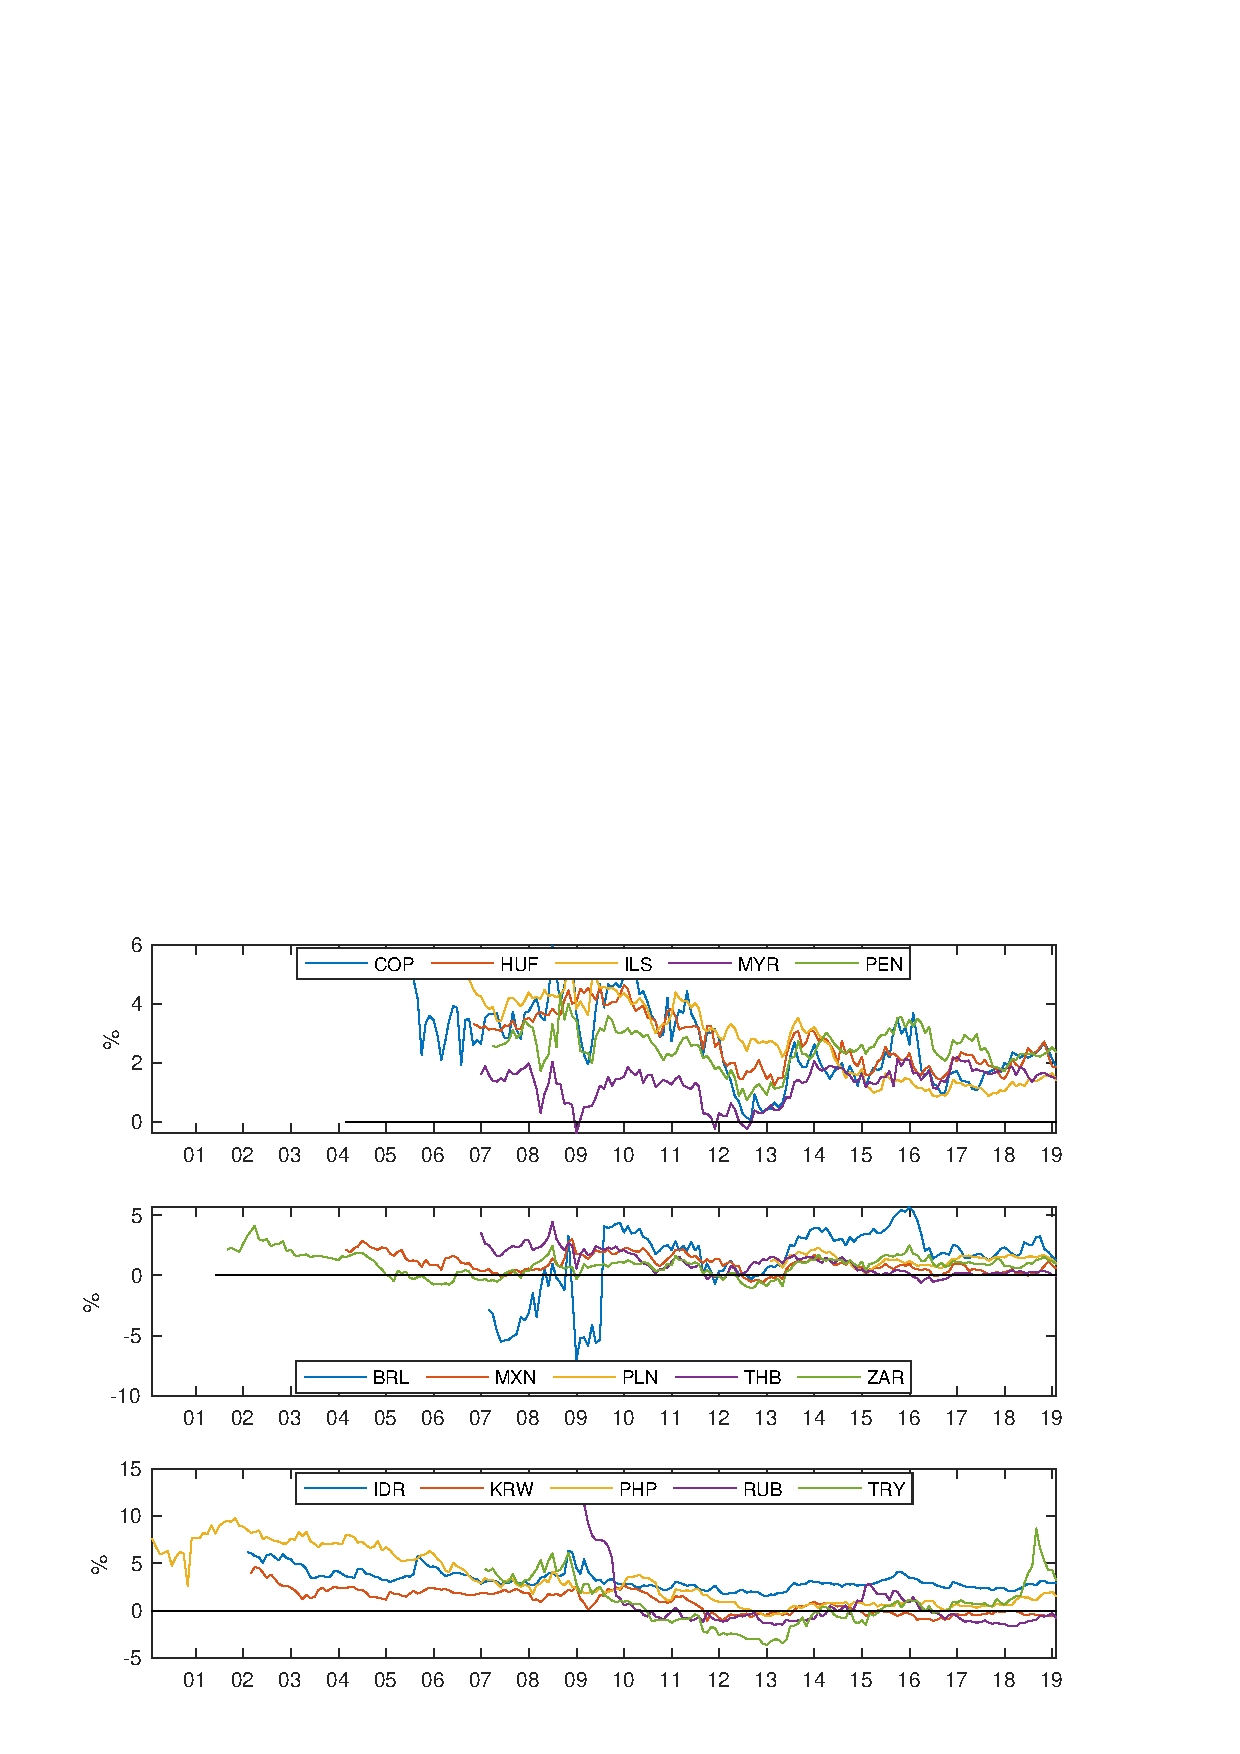
\includegraphics[width=1\textwidth,height=0.7\textheight]{../Figures/Temp/temp_tp10yrEM}
			\par\end{centering}
		\caption{Estimated 10-Year Term Premia: Emerging Markets.}\label{fig:temp_tp10yrEM}
	\end{figure}
%
%Special cases include that of Brazil whose term premium turn negative around the Great Recession and that of Russia whose term premium declined considerably. These cases might be reflecting local conditions and deserve further analysis. Consider, for example, the case of Turkey towards the end of the sample, where relevant events in 2018\footnote{On June 24, 2018, Recep Tayyip Erdogan won the presidential election. On October 2, 2018, the journalist Jamal Khashoggi disappeared after he visited the consulate of Saudi Arabia in Istanbul.} translated into a higher term premium.
%
% In addition to Brazil, Russia and Turkey, the term premia of most Asian countries has been in negative territory for some period of time. Moreover, with the exception of Brazil and South Africa, the term premia of emerging markets being negative is a phenomenon observed after the Great Recession.
%
%%To summarize the figure, Table \ref{tab:rp_stats} shows the mean of the 5-year synthetic yields and summary statistics for the estimated 5-year term premia. The means of the synthetic yields fluctuate between $2.3\%$ and $10.5\%$, while the means of the risk premia fluctuate between $-36$ basis points to $150$ basis points. On average, the term premium represents around $12\%$ of the synthetic 5-year yield. For Indonesia, Russia, South Africa and Turkey the standard deviation of their term premia is relatively high compared to their mean. Philippines and Russia had periods with a really negative term premia in October 2000 and the first half of 2015, respectively; excluding those episodes, the term premium has fluctuated between $-3.5\%$ and $5.5\%$.
%%	\begin{table}
	\centering
\begin{tabular}{l|cccccc}
\toprule
\multicolumn{1}{c}{}& &\textbf{Yield}&\multicolumn{4}{c}{\textbf{Risk Premium}}\\
\cmidrule(l{.9em}r{.9em}){4-7}
%\cmidrule(lr){3}  \cmidrule(lr){4-7}
\multicolumn{1}{c}{}&\textbf{Obs}&\textbf{Mean}&\textbf{Mean}&\textbf{Std}&\textbf{Min}&\textbf{Max}\\\midrule
{ COP}&154&6.23&1.33&1.21&-0.96&4.41\\\
{HUF}&138&3.71&0.31&0.67&-0.95&1.50\\\
{IDR}&205&8.97&0.52&1.03&-3.06&3.92\\\
{ILS}&146&2.35&1.01&0.63&0.23&2.78\\\
{MXN}&173&6.22&0.88&0.74&-0.62&2.41\\\
{PEN}&141&4.64&1.50&1.55&-3.46&5.54\\\
{PHP}&219&6.54&1.21&1.25&-11.34&3.69\\\
{PLN}&157&3.33&0.64&0.52&-0.61&1.80\\\
{TRY}&155&10.52&-0.36&1.34&-3.22&2.29\\\
{KRW}&219&3.00&0.54&0.72&-1.09&3.51\\\
{MYR}&136&2.67&0.36&0.43&-0.66&1.31\\\
{RUB}&144&7.87&-0.13&1.88&-8.87&3.90\\\
{THB}&137&2.40&0.64&0.79&-1.03&2.89\\\
{ZAR}&218&8.38&0.45&1.12&-3.02&2.25\\ \bottomrule
\end{tabular}
\\
\caption{Summary Statistics: 5-Year Yield and Risk Premium.}\label{tab:rp_stats}
\end{table}
%
%For comparison purposes, Figure \ref{fig:temp_tp10yrAE} shows the 10-year term premia estimates for advanced economies using synthetic yield curves. A clear downward trend is observed for all countries. This is consistent with the empirical evidence that uses nominal yield curves; \cite{Wright:2011} shows a declining trend in term premia for most of these countries going back to the 1990s and argues that it reflects a reduction in inflation uncertainty.
%		\begin{figure}[!htbp]
		\begin{centering}
			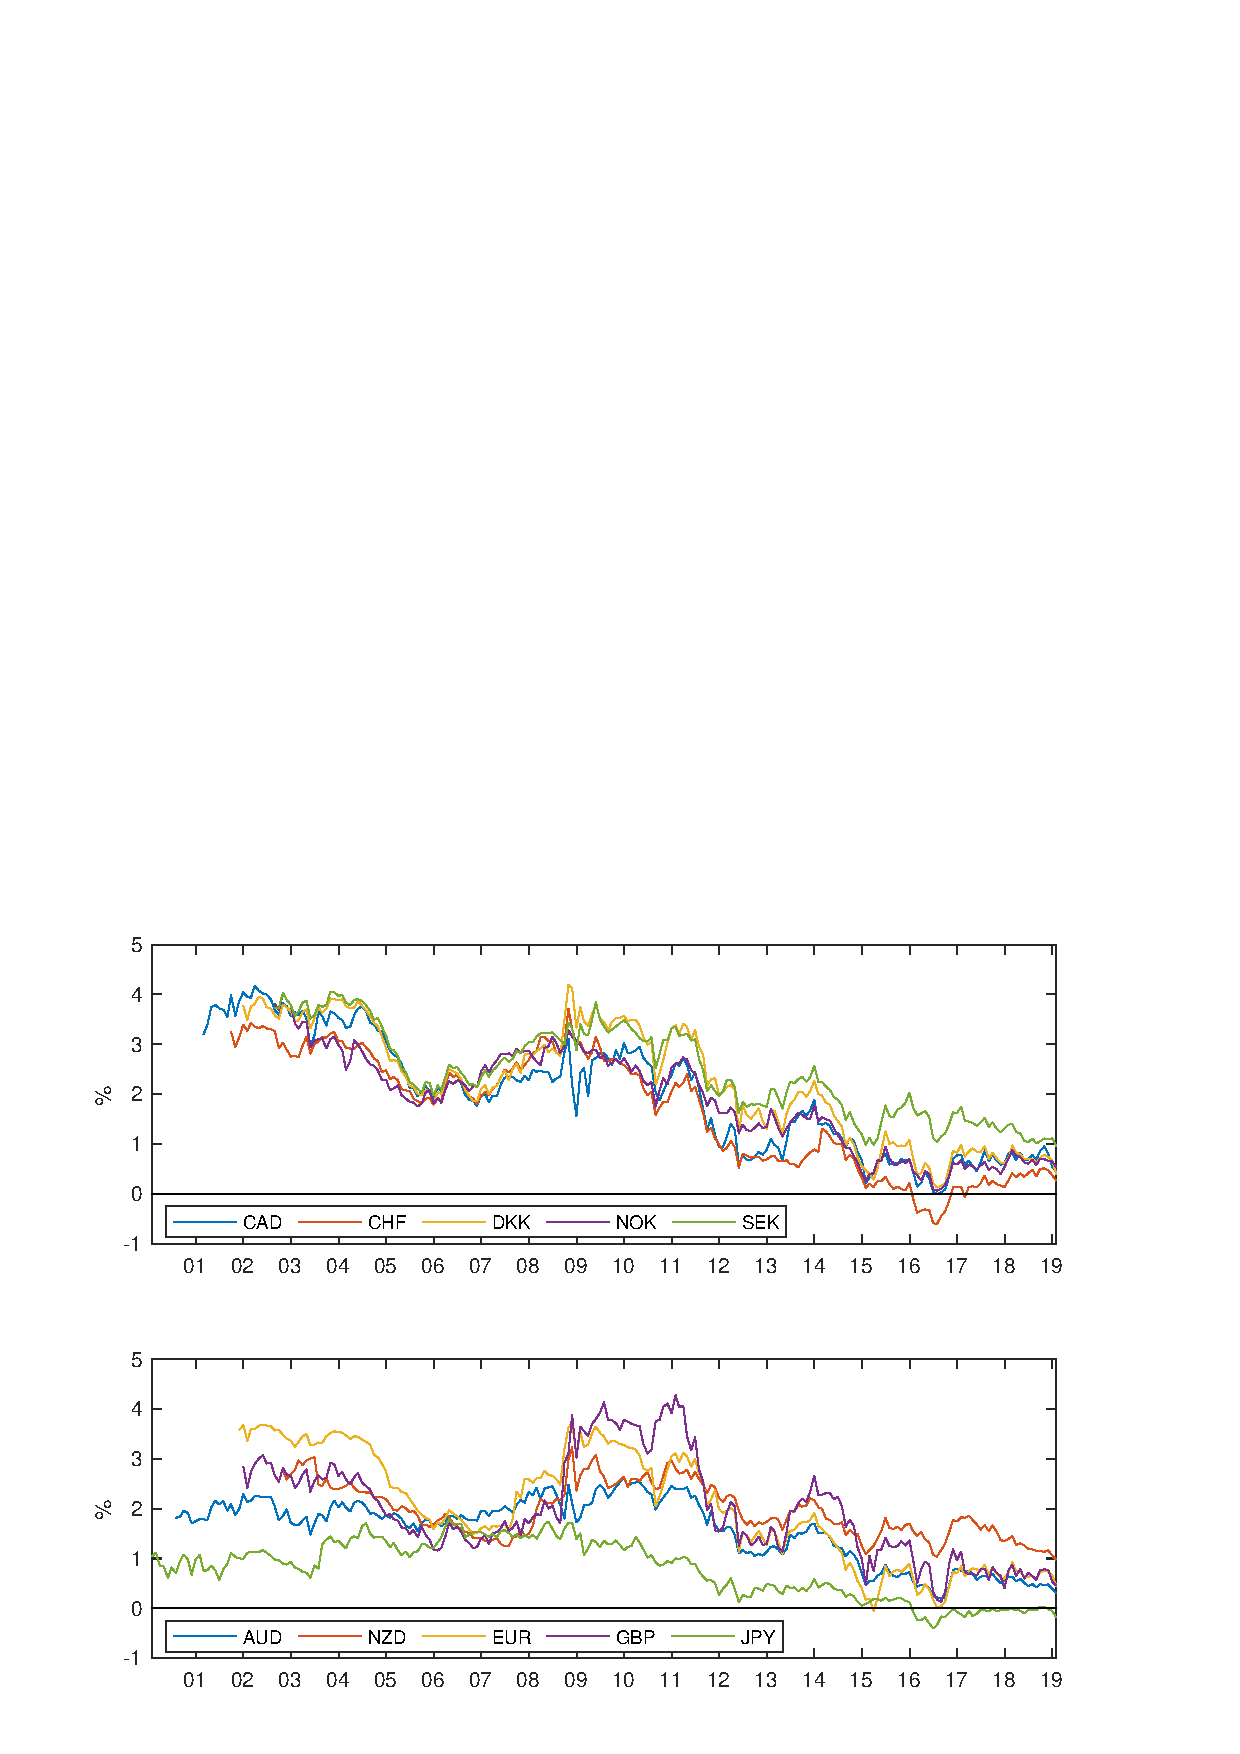
\includegraphics[width=1\textwidth,height=0.45\textheight]{../Figures/Temp/temp_tp10yrAE}
			\par\end{centering}
		\caption{Estimated 10-Year Term Premia: Advanced Economies.}\label{fig:temp_tp10yrAE}
	\end{figure}
%
%Note that although the term premia of most advanced economies seem to reflect a common factor, that of Japan behaves differently probably reflecting the fact that Japan was at the zero lower bound before the other countries.
%
%According to KW, the 10-year term premium estimate for the U.S. has been negative for most of the time since mid-2011, fluctuating between $-1$\% and $0$. Of the advanced economies considered, only Switzerland and Japan have experienced more than one month with a negative term premium, compared to several emerging markets, mainly Korea, Russia and Turkey. In particular, before the taper tantrum there was a tendency of declining term premia for emerging markets, which for some countries actually turned out negative.
%
%\subsubsection{Term Structure of Term Premia}
%In addition to comparing the term premia across countries, one can also compare them across maturities per country. In general, the term premium increases with maturity. As one would expect, when long-term bonds are seen as riskier than short-term bonds, investors would require a higher compensation for holding long-term bonds. This pattern, however, is not universal as can be seen in Figure \ref{fig:temp_ts_tp} in the Appendix, which shows two examples of this, namely Korea and Mexico. Therefore, the exceptions for the general pattern are observed in both emerging and advanced economies since the KW estimates also show that after the Great Recession, the 1-year U.S. term premium has been above the 5- and 10-year term premia at some points.
%%\footnote{Sometimes, the standard deviation of the term premia increases with maturity.}
%%		\begin{figure}[!htbp]
		\begin{centering}
			\vspace{12.5mm}
			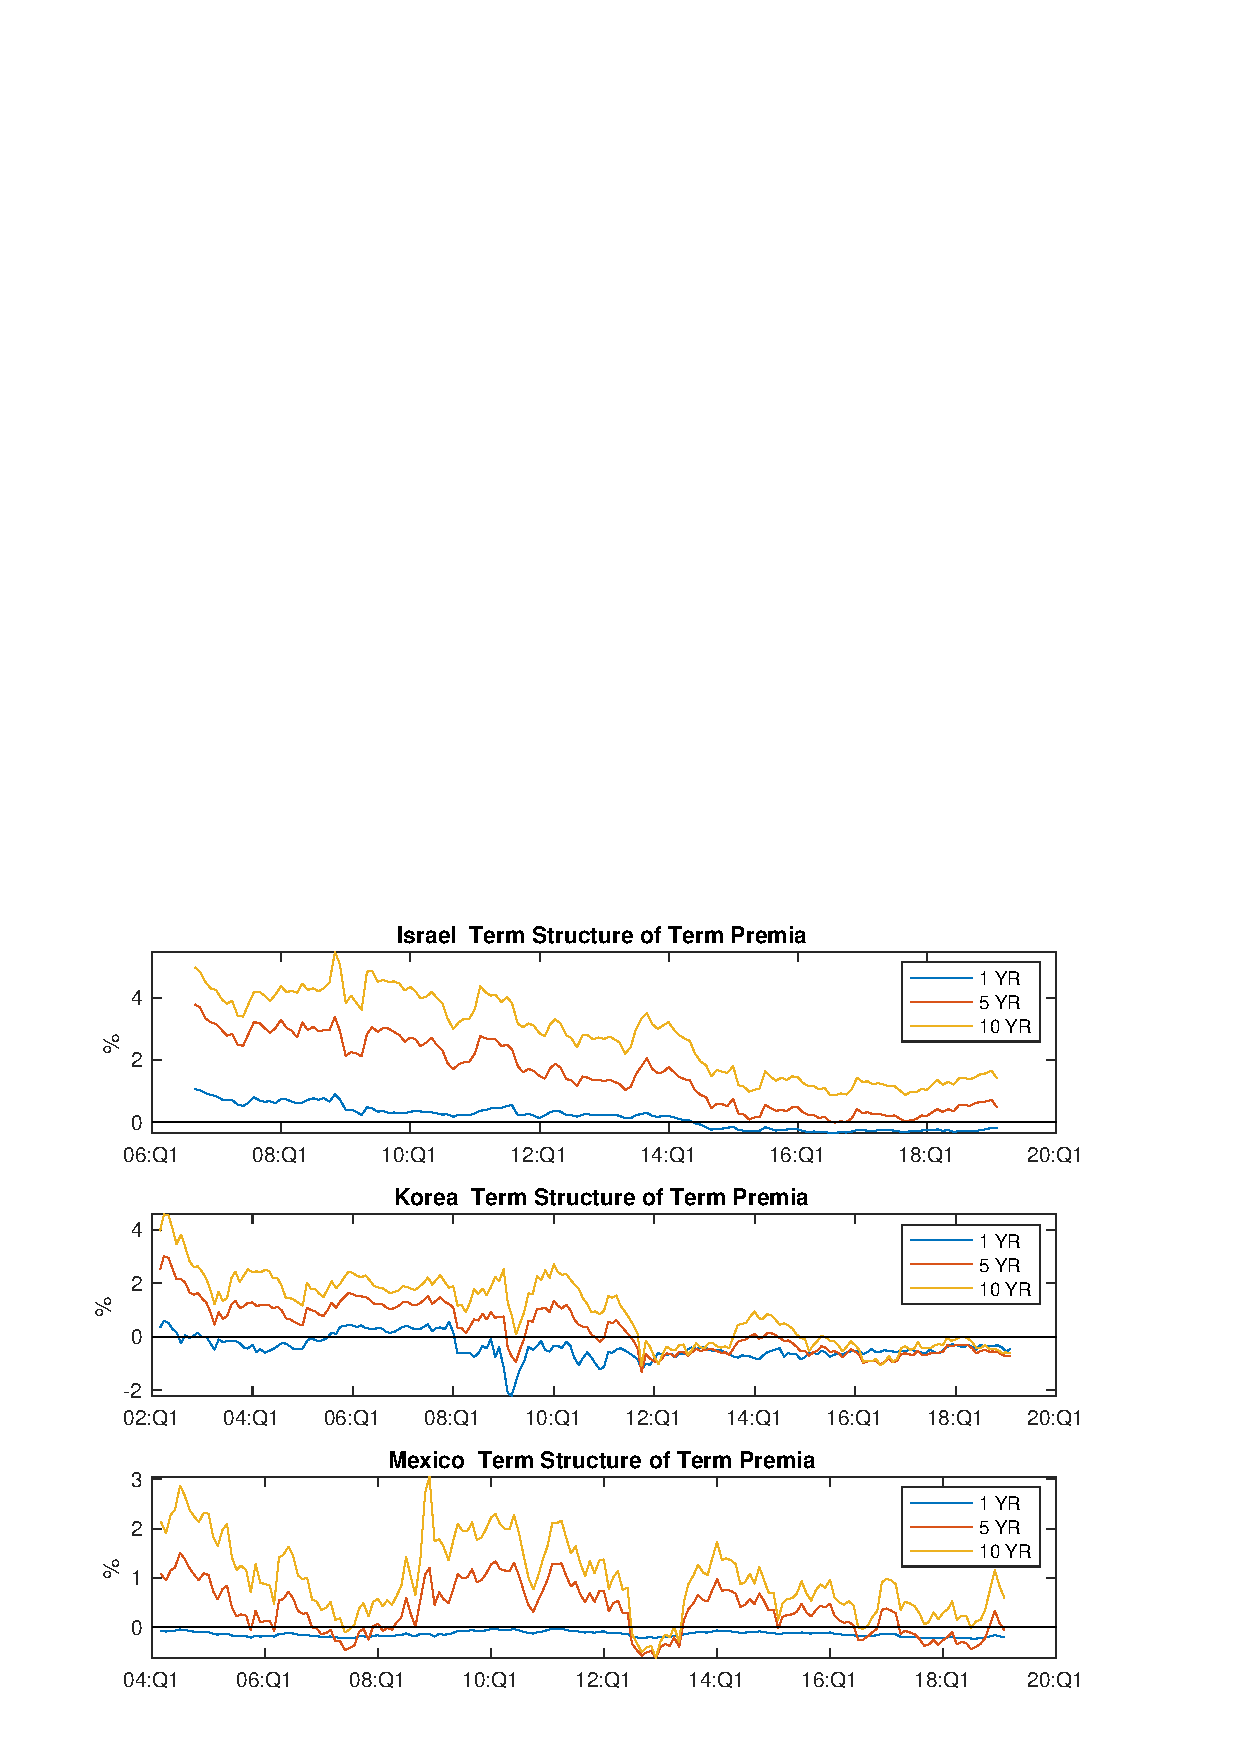
\includegraphics[width=1\textwidth,height=0.8\textheight]{../Figures/Temp/temp_ts_tp}
			\par\end{centering}
		\caption{Estimated Term Premia for Different Maturities.}\label{fig:temp_ts_tp}
	\end{figure}
%
%\subsubsection{Common Factors in Term Premia}
%To see whether there are common factors influencing the term premia in emerging markets, Table \ref{tab:temp_tp_common} shows the proportion of the total variation in the 10-year term premia explained by their first three PCs. To consider all countries, the starting date is December 2006. The first three PCs explain more than $80\%$ of the variation in the term premia of emerging markets and more than $98\%$ for advanced economies. This evidence highlights the importance of considering global factors as drivers of the term premia. But at the same time, the evidence for emerging markets shows that both domestic and common factors seem to be at play as drivers of their term premia.
%%	\begin{table}
	\centering
\begin{tabular}{l|cccc}
\toprule
&\textbf{PC1}&\textbf{PC2}&\textbf{PC3}&\textbf{Sum}\\\midrule
{ Since Nov 2016} - All Countries&40.29&23.62&12.37&76.28\\\
Since Jun 2005 - 8 countries&52.46&16.66&12.08&81.19\\ \bottomrule
\end{tabular}
\\
\caption{Proportion of Total Variance in 5yr RP Explained by First 3 PCs.}
\label{tab:pc_common}
\end{table}

%%	\begin{footnotesize}\begin{table}\centering\begin{tabular}{l|cccc}
\toprule
\multicolumn{1}{c}{} &\multicolumn{2}{c}{EM TP}&\multicolumn{2}{c}{Residual}\\
\cmidrule(l{1.1em}r{1.1em}){2-3} \cmidrule(l{1.1em}r{1.1em}){4-5}
\multicolumn{1}{c}{} & 5 YR & 10 YR & 5 YR & 10 YR \\
\midrule
(15) Dec-06 & 67.40 & 71.67 & 62.99 & 58.25 \\(8)  Jul-05 & 79.57 & 82.65 & 74.36 & 76.40 \\(4)  Latam & 95.43 & 94.96 & 94.01 & 92.47 \\(5)  Asia & 90.19 & 91.43 & 88.52 & 87.98 \\(4)  Europe & 97.38 & 95.25 & 97.15 & 93.38 \\\bottomrule\end{tabular}\caption{Percent of Total Variance Explained by First 3 PCs.}\label{table:CmnFctrs}\end{table}\end{footnotesize}
%	\begin{tiny}\begin{table}\centering\begin{tabular}{l|cc}\toprule & Dec-2006 \\\midrule EM & 81.01 \\AE & 98.07 \\\bottomrule\end{tabular}\caption{Total Variation Explained by First 3 PCs (\%): 10-Year Term Premium.}\label{tab:temp_tp_common}\end{table}\end{tiny}
%
%\subsubsection{Survey-Based Term Premia}
%As already mentioned, one way to check the term premia estimates obtained from affine term structure models is to use survey data since long-term surveys of professional forecasters can be used to obtain a model-free estimate of the long-term term premium. Using this approach, the term premium is calculated as the difference between the long-term interest rate and the survey-expectation of the future short-term interest rate over the same horizon. Since the long-term expectations of the policy rate for emerging markets are not provided by Consensus Economics, they are approximated as explained in section \ref{sec:SurveyData}. As it is also explained in that section, given the persistence of bond yields, surveys can also provide information to help in the identification of the term premium.
% It is important to acknowledge, however, that surveys might not represent the market expectations or the expectations of the marginal investor.
%
%Figure \ref{fig:temp_tp10yrSvy} displays the 10-year (long-term) term premium estimated in this way for most of the emerging markets considered in Figure \ref{fig:temp_tp10yrEM}.
%		\begin{figure}[!htbp]
		\begin{centering}
			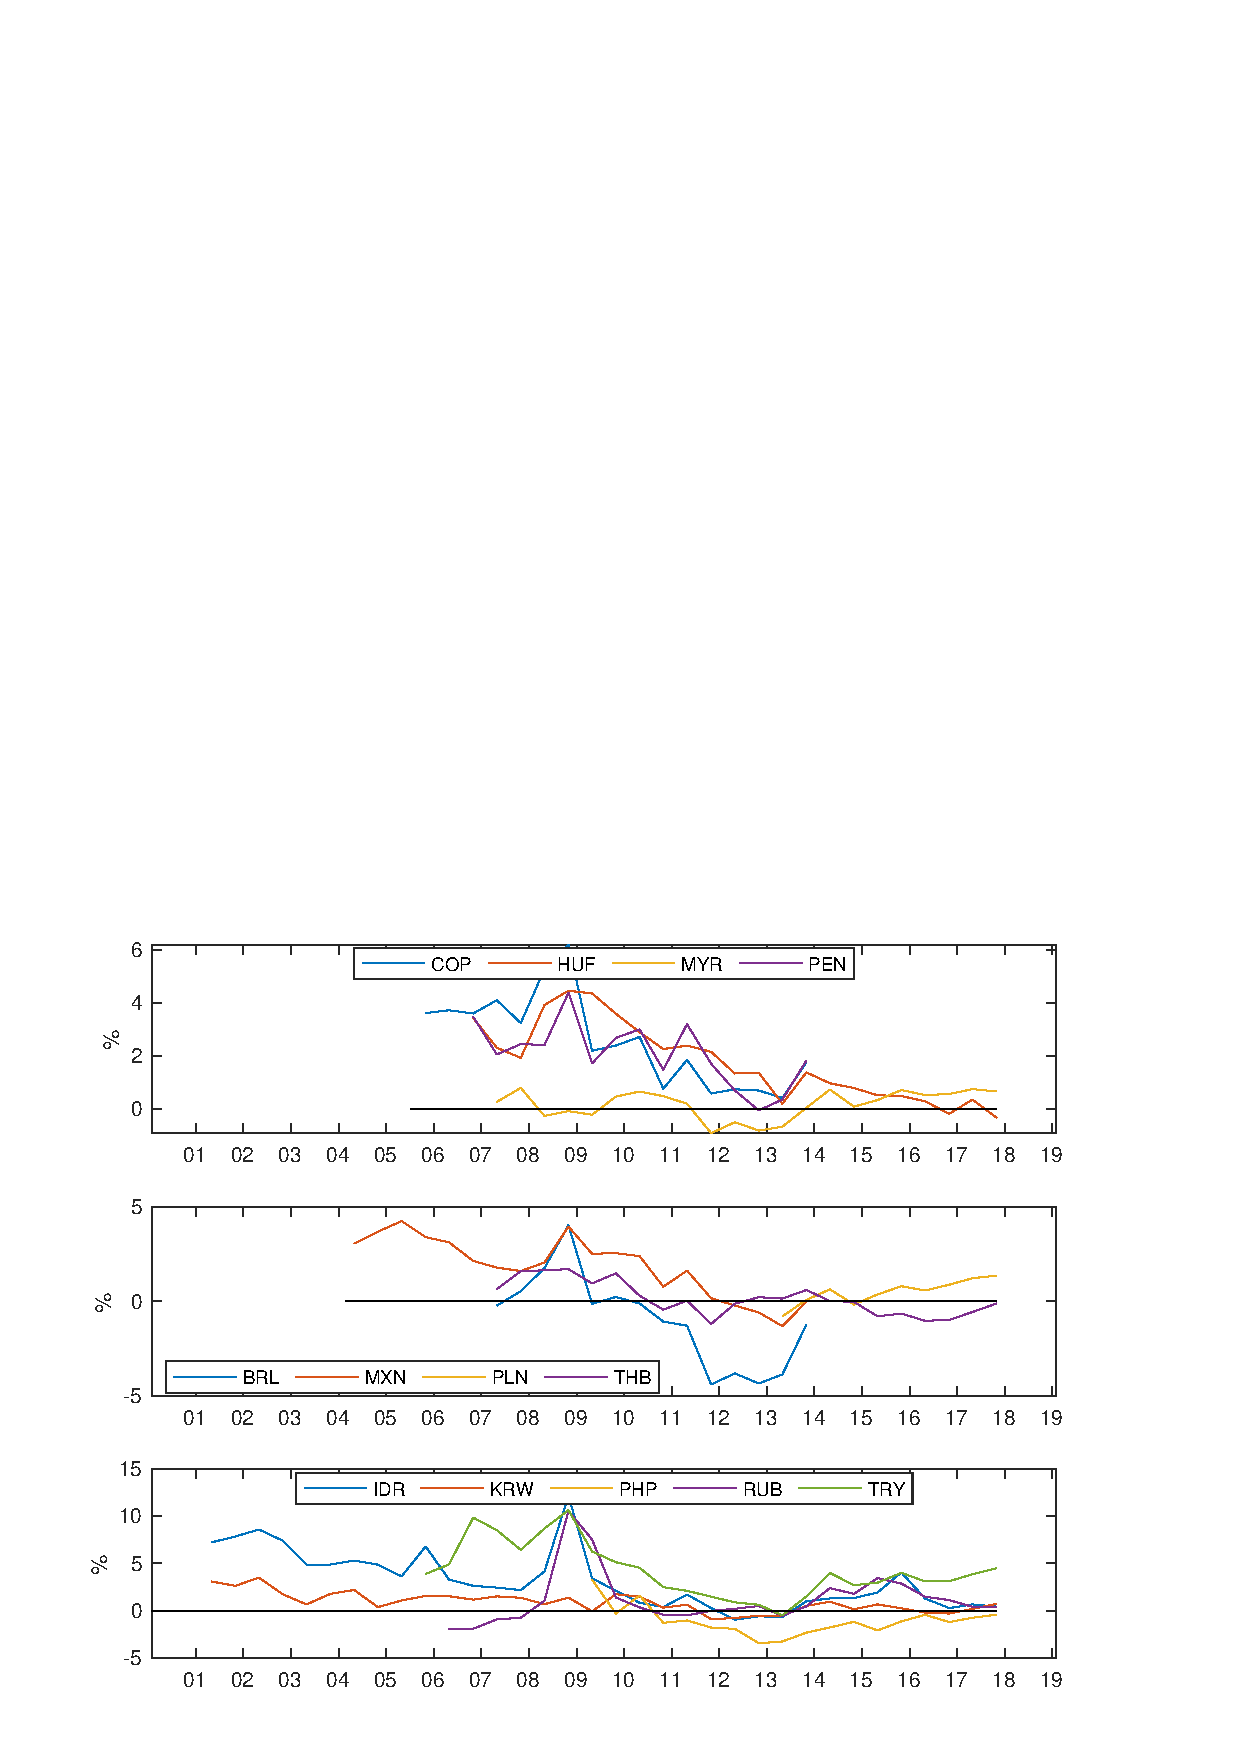
\includegraphics[width=1\textwidth,height=0.5\textheight]{../Figures/Temp/temp_tp10yrSvy}
			\par\end{centering}
		\caption{Survey-Based 10-Year Term Premium Estimates}\label{fig:temp_tp10yrSvy}
	\end{figure}
%
%With the exception of Brazil during 2012-13, the term premia estimated using survey data are in line with the model-based term premia. In fact, the average correlation between the two is $80.4\%$.\footnote{Even for the term premia calculated using the nominal yield curve, the correlation with the survey-based term premia is equal to $85\%$.} This is reassuring and supports the idea of supplementing the term structure model with survey data to better pin down the term premia in emerging markets, which will in turn provide a more robust decomposition of the nominal yield curve. This will be done in future versions of this paper.



}{}	% Closes \iftoggle{fulldraft}


\section{U.S. Monetary Policy Spillovers} \label{sec:analysis}
\iftoggle{toclinks}{\gototoc}{} % Turn it on/off in packages.tex, command in macros.tex
\iftoggle{cboxes}{	   				  % Turn it on/off in packages.tex
	\begin{boxeditems}
		\item Commonalities (TPs, yP, LCCS) all, ST vs LT.
\end{boxeditems}}{}

This section applies the decomposition described in previous sections to analyze the transmission channels of U.S. monetary policy to emerging market yields.
It provides evidence of a yield curve channel for the U.S. monetary policy.
It also documents a strong and persistent response of emerging market yields to U.S. monetary policy surprises.
%, highlighting
%It  also analyzes how each component of the yields reacts to the news, and highlights that the response
%It emphasizes 
%that yields respond differently depending on the type of surprise. %information conveyed.

\iftoggle{fulldraft}{					% Turn it on/off in packages.tex

\subsection{The Yield Curve Channel} \label{sec:Drivers}
\iftoggle{toclinks}{\gototoc}{} % Turn it on/off in packages.tex, command in macros.tex

%transmission channels of U.S. monetary surprises to EMs financial markets.
%Under an extreme case of the traditional Mundell-Fleming trilemma---the impossibility to combine free capital flows, a fixed exchange rate and an independent monetary policy---changes in the monetary policy stance in one country will have no monetary spillovers to other financially-open countries because the changes will be fully absorbed by a flexible exchange rate. %Bernanke: 
Under the traditional Mundell-Fleming trilemma---the impossibility of combining free capital flows, a fixed exchange rate and an independent monetary policy---a flexible exchange rate helps to insulate a financially-open economy from shocks abroad. %Bernanke
\cite{Rey:2013} argues that a flexible exchange rate does not fully offset those shocks because there is a global financial cycle---mainly driven by U.S. monetary policy---operating through channels other than the exchange rate, like the comovement of global asset prices and cross-border bank lending; such a cycle drives portfolio flows in or out of emerging markets, influencing their domestic financial conditions.

%The GFCy mainly influence LT rates.
%\cite{Obstfeld:2015} describes 
%One of those channels 
%Various authors have described 
\cite{Obstfeld:2015} and \cite{KolasaWesolowski:2020} describe what can be referred to as the yield curve channel of the global financial cycle.
Central banks in emerging markets can independently exert control on the short end of their yield curves, but are less powerful swaying the long end 
%of the curve 
because long-term yields are highly correlated and, thus, influenced by global forces, like U.S. monetary policy.
Accordingly, monetary policy decisions in advanced economies aimed at affecting long-term yields, like forward guidance and quantitative easing, spill over abroad via, for instance, the term premium.\footnote{ \cite{ACDM:2019} find that the correlation of the term premia in long-term yields has actually increased over the last years. \cite{Turner:2014} argues that changes in the U.S. term premium spill over into the term premia of emerging markets.}
Due to the high comovement of long-term yields, unconventional monetary policies limit the monetary autonomy of emerging markets 
%Specifically, the higher comovement among long-term rates implies that 
%Since the monetary autonomy of central banks decreases 
along the yield curve.
That is, the global financial cycle has larger effects at the long end than at the short end of the yield curve, limiting the effectiveness of domestic monetary policy to steer the economy since the entire yield curve is relevant for the spending decisions of households and firms.
%Given that the entire yield curve is relevant for the spending decisions of households and firms, stronger linkages among long-term yields across countries limit the effectiveness of domestic monetary policy to steer the economy.
%one of the goals of the unconventional monetary policy tools was to influence (decrease) long-term bond yields and, in particular, the term premium.
%the decline in monetary autonomy 
%the effects of the global financial cycle vary along the % differ / are larger / at the long end than at the short end of the yield curves of emerging markets. %\footnote{ Alternatively, the ability of the exchange rate to offset financial shocks from abroad decreases along the yield curve.}
%\cite{Obstfeld:2015} argues that %In fact, not only 
%long-term interest rates tend to be more correlated across countries than short-term rates. %, while 
%Sovereign yields are usually decomposed into a future expected short rate and a term premium.
%In addition, 
%Nonetheless, \cite{Obstfeld:2015} argues that the global financial cycle limits, rather than silence, the monetary autonomy of the central banks in emerging markets.
In addition, \cite{Kalemli-Ozcan:2019} argues that monetary autonomy is also limited at the short end of the yield curve because there are risk spillovers influencing 
%that work mainly through 
short-term yields.

\subsubsection{Comovement of Yields}
To formally assess whether different sections of the yield curves of emerging markets comove more than others, I use the connectedness index developed by \cite{DieboldYilmaz:2014}. The index assesses shares of forecast error variation in a country's bond market due to shocks arising elsewhere. 
It fluctuates between 0 and 100\%, with higher numbers indicating a higher degree of comovement.\footnote{ Following \cite{ACDM:2019} and \cite{BostanciYilmaz:2020}, I compute the connectedness index using a vector autoregression of order 1, with a forecast horizon of 10 days and a rolling window of 150 days for the daily changes of yields.} It is computed for different maturities.

Figure \ref{subfig:dy_index_tsEM} shows that among emerging markets long-term yields are indeed more connected than short-term ones, especially since the taper tantrum episode of 2013. 
Figure \ref{subfig:dy_index_tsAE} shows that the long-term yields of advanced economies are even more connected among themselves. The degree of comovement of long-term yields in emerging markets is half (around 35\%) the level in advanced economies (around 70\%),
suggesting that the medium- and long-term bonds of emerging markets are mostly held by local investors.\footnote{ According to \cite{KolasaWesolowski:2020}, the share of foreign investors in the LC bonds of emerging markets increased from 10\% in 2008 to 25\% in 2019.}
If so, local factors still play a role in explaining the long end of their curves.\footnote{ Figure \ref{fig:rolling_ts} in the appendix reports essentially the same patterns but using one-year rolling correlations of daily  yield changes at different maturities.}
%of emerging markets are far from being fully integrated in the global financial markets 
%and are therefore more responsive to local factors.

\subsubsection{Drivers of Yields}
The yield curve channel requires one to distinguish between interest rates at different maturities and calls attention to the role of the U.S. term premium.
%highlights a role to the decomposition of the U.S. yield curve---into a future expected short rate and a term premium.
%As long as LT rates respond to global factors, the effectiveness of the policy rate to steer the economy decreases.
%I focus on the yield curve channel. Under a fixed exchange rate, an emerging market essentially adopts the yield curve of the reference country. Under flexible exchange rate, the effect on the yield curve of a monetary shock abroad depends on the response of the exchange rate and the currency risk premium.
%Obstfeld: one important channel is the linkage of LT rates which reflect future expected ST rates and a term premium. 
Here I assess the role of the U.S. term premium (and of the U.S. average expected future short rates)
%and the future expected short rate ---
%its components 
in explaining the yields of emerging markets at different maturities.
Moreover, I use the three-part decomposition of those yields to see, for example, whether the U.S. term premium exclusively passes through to the term premia in emerging markets. % or to the other components too.
In fact, the assessment of the yield curve channel would be limited without the decomposition.
%only or through the other components.
%understand the direct as well as the cross effects between the expected short rates and the term premia.
For this purpose, I run the following panel regressions 
\begin{equation} \label{eq:nPanelDCMP}
	\eqpanelTPreg .
\end{equation}
\noindent in which \(\alpha_{\idxi}\) are country fixed effects, \(z^{1}_{\idxspnl}\) is a vector containing the components of the U.S. yield curve, \(z^{2}_{\idxspnl}\) is a vector of global and domestic variables that likely drive the yields, and \(u_{\idxspnl}\) is the error term. 
%for country \(\idxi\) in month \(\idxt\), 
%Fed decisions influence monetary conditions abroad \citep{Rey:2013}, its policies affect the future expected value of its policy rate as well as the compensation for interest rate risk (the term premium), whose effects can in turn spillover to domestic yields.
The dependent variables \(\yld_{\idxspnl}\) are the nominal yields and their three components 
%of the nominal yields and the forward premium\footnote{ Remember that synthetic yields add the forward premium to the U.S. yield curve.} 
for the 10- and 2-year maturities.\footnote{ \cite{Kalemli-Ozcan:2019} focuses on yields with maturities of 1 year or less. Here I focus on the 2-year yield because is a benchmark commonly used by market participants. The conclusions based on the 10- and 2-year maturities carry on if the 5- and 1-year maturities are used instead. Appendix \ref{sec:AppTables} reports the results for the 5- and 1-year maturities. The 1-year maturity is the shortest one for which the decomposition of the U.S. yield curve used here is available.}
%, namely the expected future short rate, the term premium and the credit risk compensation. 
%The dependent variable in the last column of the table is 
%, and so it is included to assess whether its behavior mirrors that of any of the components.
%As can be seen, the components have different dynamics, they are not associated to the same variables nor in the same magnitudes.
%Also, none of them can be inferred from the forward premium as it behaves differently to %does not mirror % directly tied to 
%any of them.
As before, I use Driscoll--Kraay standard errors to test for significance.\footnote{ The Pesaran test of cross-sectional independence is rejected in all cases at the 1\% significance level.} %\cite{DriscollKraay:1998}
%estimator that allows the errors to be correlated across countries and over time 
% Lag selection based on Newey \& West(1994) “plug-in” estimator
%Automatic lag selection in covariance matrix estimation. Review of Economic Studies 61: 631–653.

%To what extent US YC is related to EM yield components?
%Potential drivers of the yields of emerging markets included in vector \(z_{\idxspnl}\) are the following.

%Synthetic yields are constructed from the U.S. yield curve, so movements in the latter will likely influence the yields of emerging markets.
%Moreover, decomposing the U.S. yields can be even more insightful.
%will more generally is one of the potential drivers of 
%I start by studying the role of the components of the U.S. yield curve as drivers 
%cyclical properties of the nominal yields 
%To do this, 
The explanatory variables of interest come from the decomposition of the U.S. yield curve based on the \cite{KimWright:2005} model, which 
%decomposes the yields into an expected future short rate and a term premium, and 
addresses the small sample problem using survey forecasts of future interest rates.
%start the analysis of the relationship between U.S. monetary policy and the sovereign yields of emerging markets, I run panel data regressions of those yields on the components of the U.S. yield curve controlling for a variety of  variables.
%At the same time, those regressions allow me to study the cyclical properties of  emerging market yields. The coefficients of interest are those associated with 
I control for the monetary stance and local macroeconomic conditions using the policy rate reported by each country to the Bank for International Settlements, as well as domestic inflation and unemployment rates. %in each country
\cite{Rey:2013} highlights the role of the Cboe's volatility index (Vix) as an important driver of the global financial cycle,
%Other potential drivers of emerging market yields include 
%global financial and domestic macroeconomic and financial variables.
%The variables considered to capture global financial conditions are 
% and the S\&P \(500\) stock market index. 
%The Vix 
it reflects the implied volatility in stock option prices and is usually seen as a measure of risk aversion and economic uncertainty.\footnote{ Given the sudden spikes in the index, it is common to use it in logs. For consistency, the other uncertainty indexes are also used in logs.}
\cite{BakerBloomDavis:2016} construct a news-based economic policy uncertainty (EPU) index that serves as the basis for the global and U.S. versions,\footnote{ Although the EPU index has been replicated for different countries, it is only available for five of the emerging markets in the sample: Brazil, Colombia, Mexico, Russia and South Korea.} %, which would allow to account for domestic political uncertainty.
which are used as alternative, and arguably exogenous, measures of global uncertainty.
The index of global economic activity %based on world industrial production 
proposed by \cite{Hamilton:2019} captures real variables. % are the price of oil and 
%The VIX and the federal funds rate have been used in the global financial cycle literature \citep[see][]{Rey:2013} to study the effects of common factors on capital flows. The VIX is usually used as a measure of risk aversion and economic uncertainty and the fed funds rate is a measure of the monetary policy stance in the U.S. 
%For the U.S. monetary policy, the variable used is the effective federal funds rate calculated by the New York Fed.
%year-on-year percentage change in the consumer price index
%The domestic variables include inflation, the unemployment rate and industrial production to capture macroeconomic effects. 
Finally, the exchange rate (LC per USD) is included to rule out explanations of changes in yields based on currency movements; the exchange rate is standardized for each country over the sample period.
%and the local stock market index are included as measures of local financial conditions.
%Monthly returns for the stock market index, the oil price and the exchange rate are calculated as the log difference of the series, and expressed in basis points.

Tables \ref{tab:ycdcmp10y} and \ref{tab:ycdcmp2y} report the results.
The evidence is in line with the yield curve channel.\footnote{ The tables report the estimates for the full specification of the model. The results are robust to specifications of the model that progressively include the regressors for each dependent variable.} 
%that includes all of the potential drivers.
%In terms of drivers, 
First, the response of the average expected future short rates of emerging markets to the domestic policy rate decreases with maturity and is positively associated with its U.S. counterpart only at the long end, both results are in line with the argument that monetary autonomy is stronger at the short end than at the long end of the curve.
Second, the response of the term premia of emerging markets to the U.S. term premium increases with maturity and is positively associated with the Vix only at the long end, both results consistent with the claim that the U.S. term premium, and the global financial cycle in general, is more relevant for the long end than for the short end of the curve. 
Third, the U.S. term premium not only influences the yields in emerging markets through its effect on their term premia but through the other components too.
%More generally, there are direct and cross effects between the expected short rates and the term premia.
In particular, I can directly test the thesis in \cite{Kalemli-Ozcan:2019} regarding risk spillovers to the short rate thanks to the yield decompositions.
Indeed, these risk spillovers to the average expected future short rates of emerging markets decrease with maturity and operate through 
%; the results further reveal that those risk spillovers are due to 
the U.S. term premium rather than the Vix.
%Lastly, here is where accounting for credit risk pays off; when it is ignored, the conclusions on direct and cross effects between the components of the yields change. Why? Because the resulting `term premium' mixes together a pure term premium and a credit risk compensation.
These conclusions would be different if we failed to account for credit risk and thus merged the term premium and credit risk components.

%Over the course of the month CR flips sign wrt on-impact
%K-O: Strongest response of YP at short end
%USTP affects all 3 components
%CBP small effect on CRC
%Inflation increases CRC at medium and long end
%Unemployment increases TP at medium and long end
%Depreciations reduce CIP deviations
%For TP matters EPU US at short end but Vix at long end
%No effect of Vix on TP at sort end


%The role of the components of the U.S. yield curve %play a significant role for emerging market yields, highlighting the 
%already indicate potential spillover effects from the Fed's policy decisions to emerging market yields.
%%It is worth highlighting here the direct link between the equivalent components. 
%Increases in the future expected short rate in the U.S. are positively associated with future expected policy rates in emerging markets, whereas increases in the U.S. term premium relate to increments in the term premia of emerging markets.
%Moreover, the association between the U.S. components and the synthetic yields is larger than with the nominal yields. This in turn explains the negative association of the U.S. components with the credit risk compensation.
%Larger increases in synthetic relative to nominal yields, mechanically decrease the credit risk compensation.
%Therefore, the trade-off between explicit and implicit defaults highlighted before can be seen in table \ref{tab:ycdcmp10y} through the connection between the U.S. term premium and the credit risk compensation.
%In addition, there are also cross effects. 
%The expected short rate in emerging markets reacts to changes in the U.S. term premium. 
%This is consistent with the U.S. risk spillovers channel described by \cite{Kalemli-Ozcan:2019}.
%The signs for the rest of the drivers are reasonable.


%More generally, external conditions have a relevant impact on domestic bond markets, consistent with the view of a global financial cycle.
%The U.S. term premium, the Vix and the U.S. stock market are linked to the different components of emerging market yields.\footnote{ On the other hand, once controlling for the other factors, the price of oil and the global EPU index play no role in explaining yield dynamics.}
%They are particularly associated with the credit risk compensation, 
%%is global financial conditions given by the Vix, the U.S. term premium and the U.S. stock market.
%but they do not seem very helpful in providing information about default risk in emerging markets given their low explanatory power (in terms of the R-squared statistic) relative to the other yield components.
% since  explain a relatively lower percent of the premium's variability.

%In this case, the effect is similar among all countries.
%On average, the 10-year U.S. term premium explains around 40\% of the variation in the expected short rates in both EMs and AEs.
%Moreover, for EMs, the 10-year U.S. term premium explains more of the variation of the expected short rate than the U.S. expected rate itself. % unlike the case for AEs before GFC
%After the GFC, the 10-year U.S. term premium explained more than the U.S. expected rate in both AEs and EMs.

A glimpse on the drivers of the yields of emerging markets is a byproduct of the analysis on the yield curve channel.
%on understanding
%The results for the rest of the drivers are reasonable.
%TP countercyclical
%TP and inflation. Inflation mainly affects TP
%Unemployment mainly affects CRC. 
%Vix only affects TP and CRC (not YP)
%US uncertainty increases CRC. 
%Vix effect on CRC is larger.
%HHS risk taking channel. Depreciations increase yields due to YP and TP
For instance, inflation and unemployment are key domestic variables.
%The evidence in table \ref{tab:ycdcmp10y} suggests that t
In particular, the term premium and the credit risk compensation seem to be countercyclical, investors demand higher compensations during recessions, when the unemployment rate increases. 
Moreover, the positive association between inflation and the term premium conforms with the idea that inflation erodes the value of nominal bonds and so, in periods of rising inflation investors expect the central bank to tighten its monetary stance going forward, demanding a higher term premium. 
%More generally, changes in inflation are associated with changes in all of the dependent variables except for the credit risk compensation. 
%In particular, the magnitudes are similar for nominal and synthetic as well as for the forward premium.
As expected for measures of risk and uncertainty, shifts in the Vix are positively associated with the term premium and credit risk compensation, but not with the expected future short rate.
Also, higher economic uncertainty in the U.S. seems to induce a flight to quality in the short end of the yield curve and a reduction in the perceived credit quality.\footnote{ The coefficient for the U.S. EPU index in the term premium column is negative and positive in the credit risk compensation column.}
Lastly, there is evidence supporting the risk-taking channel of exchange rates,\footnote{ According to the standard trade-channel effect, an appreciation is contractionary because it discourages exports and stimulates imports, reducing the trade balance.} 
according to which a currency appreciation is associated with easier financial conditions (and compressed sovereign bond spreads) due to balance sheet effects.
However, here it works through the expected future short rate and the term premium rather than through the credit risk compensation as reported by \cite{HofmannShimShin:2019}.
%The two main domestic factors are . Holding the other factors constant, an increase in any of these three variables increases the term premia in emerging markets. 
%The effect of the domestic variables is in line with what has been found for advanced economies using nominal yield curves. 

So far, the yield decompositions have been valuable to assess the validity of the yield curve channel and understand the driving forces behind the sovereign yields of emerging markets.
Notwithstanding, 
%it is important to acknowledge that 
the specification in equation (\ref{eq:nPanelDCMP}) may suffer from econometric problems such as persistent variables, reverse causality and omitted variables.
Moreover, the measures of comovement are unconditional, and so not specifically driven by monetary policy surprises. % but are rather calculated for all yield curve movements.
%In addition, the sample period includes few U.S. policy rate surprises. %; in fact, most monetary policy decisions operated not through changes in the policy rate.
%These issues are addressed next.


%
%To compare how interconnected are the yields of emerging markets relative to the yields of advanced economies, I use the connectedness index developed by \cite{DieboldYilmaz:2014}, which essentially assesses the degree to which a shock in one country spill over to other countries.
%%between the yields of different maturities varies 
%%\cite{DieboldYilmaz:2014} propose a system-wide measure of connectedness 
%%based on forecast error variance decompositions.
%%Their methodology 
%%assesses shares of forecast error variation in a country's bond market due to shocks arising elsewhere.
%The connectedness index fluctuates between 0 and 100 percent, with higher numbers indicating a higher degree of comovement.\footnote{ Following \cite{ACDM:2019} and \cite{BostanciYilmaz:2020}, I compute the connectedness index using a vector autoregression of order 1, with a forecast horizon of 10 days and a rolling window of 150 days for the daily changes of yields.} 
%%for each of several maturities.
%%the 10-year nominal yield
%%%of the emerging markets in the sample 
%%and each of its components.
%%Figure \ref{fig:dy_index_ts} plots the connectedness index for different maturities.
%Figure \ref{subfig:dyindexTSEM} plots the connected index for the nominal yields of both groups of countries and for the synthetic yields of emerging markets.
%%It shows that the long end is indeed more connected than the short end in advanced economies and more recently in emerging markets---since the taper tantrum episode of 2013.
%Although the connectedness of the short end is similar between the two groups of countries, the degree of comovement of the long end in emerging markets is half (around 35\%) the level of advanced economies (around 70\%).
%The difference in connectedness 
%%between the two groups of countries 
%is therefore driven by the medium and long end of their yield curves.



\subsection{Identification of Monetary Policy Surprises} \label{sec:USMPS}
\iftoggle{toclinks}{\gototoc}{} % Turn it on/off in packages.tex, command in macros.tex

%This section first explains how the monetary policy surprises are calculated and then analyzes the responses of emerging market yields to those surprises.

Surprises in monetary policy decisions are identified using intraday data on asset prices around the Fed's monetary policy announcements in order to capture changes in the information set of market participants. %\citep{GurkaynakWright:2013,NakamuraSteinsson:2018JEP}
%The construction of the surprises therefore requires to calculate changes in asset prices that capture market expectations of monetary policy decisions.
%These changes are measured in windows containing monetary policy decisions
Asset price changes are calculated from 15 minutes before to 1 hour and 45 minutes after each Federal Open Market Committee (FOMC) meeting since 2000 giving a total of 162 events.\footnote{ Following \cite{GSS:2005a}, I exclude from the analysis the meeting of September 2001 that followed the terrorist attacks in New York.}
The surprises are set to zero in non-announcement days. %FOMC meeting 
Neither minute releases nor speeches by Fed officials are included. 
%, only (scheduled and unscheduled) monetary policy announcements.
%Unlike \cite{FerrariKearnsSchrimpf:2017}, who include releases of minutes and speeches by Fed officials, the dataset here includes monetary policy announcements only.

\cite{GSS:2005a} and \cite{Swanson:2018} show that monetary policy has more than one dimension. Asset prices respond to different types of news about monetary policy.
Following \cite{RogersScottiWright:2018}, I consider three separate types of U.S. monetary policy surprises,
%unexpected changes to the current policy rate \citep{Kuttner:2001}, surprise changes to the future path of the policy rate \citep{GSS:2005a}, and unanticipated announcements about the Fed's LSAP programs \citep{Swanson:2018}. They will be 
referred to hereinafter as target, forward guidance and asset purchase surprises.
%To compute the surprises, I use the current federal funds rate future (FF0) contract, the 8-quarters ahead eurodollar future (ED8) contract and the yield of the 10-year U.S. Treasury bond.
The target surprise is the change in the yield on the current- or next-month federal funds futures contracts, as proposed by \cite{Kuttner:2001}.
%uses rescaled changes in the price of the FF0 contract as in \cite{GSS:2005a}, who implement an intraday version of the daily measure proposed by \cite{Kuttner:2001}.
%Price changes in the 8-quarters ahead Eurodollar future contract measure surprises in the federal funds rate two years into the future.
The forward guidance surprise is the residual from regressing the yield change of the 8-quarters ahead Eurodollar futures contract on the target surprise.\footnote{ The yield change of the 4-quarters ahead Eurodollar futures contract could also be used to capture the forward guidance surprise. However, intraday changes in that contract became essentially zero after 2011 since market participants expected the policy rate to remain at zero for at least a year. Eurodollar futures contracts are bets on the future level of 3-month interest rates.}
%ED8 contract on the target shock, and is highly correlated with the forward guidance factor in \cite{GSS:2005a}.
%Finally, %in line with \cite{Swanson:2018}, %for measuring the last type. % of surprises.
The asset purchase surprise is the residual from regressing the yield change in the 10-year Treasury futures contract on the target and forward guidance surprises.
%By construction, the surprises are uncorrelated.
A positive value in any of the surprises represents a tightening of the monetary policy stance, and vice versa.
%whereas a negative shock indicates an easing.
%Correlation of surprises?

%Sample periods for the surprises.
The relevance of the surprises has varied over time.
After 2008, there were no changes in the current policy rate until %the first rate hike in 
December 2015, so target surprises were essentially zero during that period.
Meanwhile, asset purchase surprises are considered starting in October 2008 because their meaning is unclear before that date.
Forward guidance surprises have nevertheless been relevant before and after the global financial crisis. %\footnote{ In general, the surprise is set to zero in non-announcement days or in periods outside of the considered range (e.g. before October 2008 for asset purchase surprises).}
%As a result, target surprises are only considered from 2000 to 2008 and again starting in December 2015, asset purchase surprises are considered from October 2008 onwards, while forward guidance surprises span the whole sample period.
%Figure \ref{fig:USmps} plots all three monetary policy surprises.
Table \ref{tab:mpsstats} in the appendix reports descriptive statistics for the three types of surprises. %on monetary policy announcement days.
%magnitude of surprises is generally less than 10 basis points.
%; notwithstanding, there were large easing forward guidance and asset purchase surprises on March 18, 2009.
In general, the Fed has been more aggressive in stimulating than in contracting the U.S. economy, since easing surprises are larger on average and more common than tightening surprises.


\subsection{The Effects on Emerging Market Yields} \label{sec:LPs} %\label{sec:spillovers}
\iftoggle{toclinks}{\gototoc}{} % Turn it on/off in packages.tex, command in macros.tex

The transmission of U.S. monetary policy to the yields of emerging markets is assessed using panel local projections for the daily changes in the 
%yields and their components.
yields.\footnote{ \cite{Jorda:2005} advocates the use of local projections as an alternative to VAR models in order to generate impulse responses that are robust to misspecification. See \cite{HofmannShimShin:2019} and \cite{ACDM:2019} for recent applications of panel local projections.}
While event studies report the response of the variables on the day of a surprise,
local projections %are preferred in this context because they 
additionally provide the responses over subsequent periods.
%This is especially important for emerging markets.
It is important to be able to capture the persistence in the response of emerging market yields given the pervasive post-announcement drift in the bond markets 
%in the U.S. and other 
of advanced economies documented by \cite{BrooksKatzLustig:2019}.
To better understand the transmission of the Fed's decisions to the yields, I leverage on the yield decompositions at the daily frequency. %of emerging markets.
%the decomposition of emerging market yields is key  surprises in U.S. monetary policy to the yields. %better characterization of the response.
%to understand the spillover effects of the Fed's decisions on 

Specifically, I run the following panel local projections:
	\begin{equation} \label{eq:nPanelLP}
	\eqpanelLP,
\end{equation}	% \ref{eq:nPanelLP}
\noindent in which 
%\(\idxi\) and \(\idxt\) are respectively the country and time indexes, 
\(\idxh\) indicates the horizon (in days) with \(\idxh = 0, 1, \ldots, 45\) and each \(\epsilon^{j}_{\idxt}\) represents one of the three types of monetary policy surprises.\footnote{ There is no need to control for past or future surprises since, by definition, they are unanticipated by the market. On the other hand, even though the types of surprises are uncorrelated by construction, the estimation is more efficient when all the surprises are included simultaneously.} %although there is no need to control for the other (since they 
The regressions include country fixed effects \(\alpha_{\idxh,\idxi}\), a lag of the dependent variable,\footnote{ As argued by \cite{HofmannShimShin:2019}, the large number of daily observations reduces the potential for Nickell bias that arises by including a lagged dependent variable in panel regressions with fixed effects and small time dimensions. Indeed, the impulse responses reported here are essentially the same when the lag of the dependent variable is excluded.} % and \(u_{\idxspnlfwd}\) is the error term.
and a lag of the exchange rate \(\fx_{\idxspnllag}\). % (expressed in LC per USD).
The regressions are ran for the 10- and 2-year nominal yields and each of their components.
%(the expected short rate, the term premium and the credit risk compensation) 
%for every type of monetary policy surprise.
The confidence bands are constructed using Driscoll--Kraay standard errors, which allow for time and cross-sectional dependence.
% Lags for DK in LPs: 9

The parameters of interest, \(\beta^{j}_{\idxh}\), measure the average response of the nominal yield (or its components) to monetary policy surprise \(j\) at horizon \(\idxh\). 
The contemporaneous effects (when \(\idxh = 0\)) are marked with an arrow in the figures below.
All responses are assessed relative to a one basis point reduction (an easing) in any of the surprises, since the Fed has been more aggressive in that direction during the sample period.

The response of the U.S. yields and its components to the three surprises serves as a benchmark to assess the responses of the yields of emerging markets. 
As before, the U.S. yields come from the dataset of \cite{GSW:2007}, and the components from the decomposition proposed by \cite{KimWright:2005}.
The responses are reported in figures \ref{fig:LPUStarget} to \ref{fig:LPUSlsap} in the appendix. 
They are consistent with the findings in the existing literature.
%In general, Fed's decisions impact both expectations about its policy rate in the future and the compensation required by investors to hold long-term bonds.
%The first column of figures \ref{fig:LPUS2Y} and \ref{fig:LPUS10Y} shows the responses of the 2- and 10-year yields, respectively, to all three surprises.
%The on-impact effect of the 2-year yield to any of the three surprises is similar at around %half a basis point increase.
%5 basis points for a 10 basis point increase in any of the surprises.
%By contrast, the 10-year yield only increases in response to forward guidance and asset purchase surprises contemporaneously, with asset purchase surprises having a more than one-to-one impact.
%The magnitudes are in line with previous literature.
%The duration of the effects ranges from a couple of days up to a few days past a month, where 
%the delayed response can be larger that the initial reaction, consistent with the evidence in \cite{BrooksKatzLustig:2019}.
%The decomposition allows for a better characterization of the response.
For instance, target easing surprises reduce yields, mainly driven by a decline in the average expected future short rates;
while forward guidance and asset purchase easing surprises decrease yields, in part due to a reduction in the term premium.
%Moreover, the responses build over time in all cases.
%one of the goals of the unconventional monetary policy tools was to influence (decrease) long-term bond yields and, in particular, the term premium.
% \citep[see][]{Kuttner:2018}.
%\footnote{ \cite{Kuttner:2018} discusses the effects of the QE announcements on U.S. bond yields.}
%The right hand panels in figures \ref{subfig:LPUS10Ypath} and \ref{subfig:LPUS10Ylsap} confirm this.
%Meanwhile, the main effects of target surprises are seen on the expected short rate, especially at the 2-year maturity (middle panel of figure \ref{subfig:LPUS2Ytarget}).
%Target surprises did not influence the 10-year yield.


\subsubsection{Target Surprises}
\iftoggle{toclinks}{\gototoc}{} % Turn it on/off in packages.tex, command in macros.tex

%W/o decomposition, could only assess the YC channel by looking at nominal yields only.
Figure \ref{fig:LPEMtarget} shows the response of the yields of emerging markets to a target easing surprise.
The magnitude of the contemporaneous yield response %of the  yields in emerging markets 
is lower than in the U.S., but it builds over time.
This delayed response is documented by \cite{BrooksKatzLustig:2019} for the U.S. and by \cite{ACDM:2019} for a sample comprised mostly of advanced economies,\footnote{ It is also seen in the responses of U.S. yields reported in appendix D.} which \cite{BrooksKatzLustig:2019} attribute to a portfolio rebalancing channel.
%, it can last for up to 2 months and intensify to such an extent so as to become a one-to-one response, or even more in the case of asset purchase surprises.
%In particular, the path and asset purchase surprises have a larger and longer effect on EM yields. 
%The response of yields of emerging markets therefore lasts relatively longer than the response of U.S. yields.
%As will be discussed in the next two subsections, there is also a 
%The evidence documented here is also consistent with said channel.
Moreover, the reaction to forward guidance and asset purchase surprises is also sluggish, as discussed later.
Therefore, slow-moving capital is also present in emerging markets.\footnote{ Figure \ref{fig:LPEMRHO} in the appendix shows that the delayed responses are not driven by the response of the forward premium, the term added to the U.S. yield curve to construct the synthetic yields.} %a decline in the forward premium (when the spot is higher than the forward) implies a future expected appreciation of the domestic currency.


Following a target easing surprise, both the U.S. and emerging market yield curves steepen. %because 
The surprise reduces the short but not the long end of the yield curves in such a way that the long end of the synthetic yield curve declines by more than the nominal one. 
That is, borrowing long-term in LC synthetically becomes cheaper; equivalently, the opportunity cost of lending long-term directly in LC increases.
As a result, the credit risk compensation at the long end rises %increases 
by almost one-to-one in the month following the surprise. %1 basis point one month after a 1 basis point surprise.
%Intuitively, the surprise reduces relatively more than directly, increasing 
The surprise therefore seems to trigger capital flows towards emerging markets that slowly concentrate on short term LC bonds.
This would explain the effect on long-term credit risk compensation, which declines on impact but increases over the month following the surprise. % reverses
%In addition, figure \ref{fig:LPEMtarget} %the three-part decomposition of the yields 
Credit risk compensation is thus an important factor to understand %that needs to be taken into account when assessing 
the transmission of U.S. monetary policy to emerging markets.
%The response of the long-term yield is not statistically significant.
%In fact, due to a decline in the ST yield.
%One implication of the yield curve channel is that central banks in emerging markets are limited to influence the long end of their yield curves following a monetary policy surprise in the U.S.
%Figure \ref{fig:LPEMtarget} also indicates that the response to a target % easing surprise 
%Figure \ref{fig:LPEMtarget} helps to understand the effects of a target surprise in emerging markets.
Nevertheless, the response of their yields %in emerging markets 
to a target easing surprise is also driven by the expected short rate; in particular, %reflecting 
investors expect for central banks in emerging markets  to follow the U.S. monetary stance. %Fed's decision.
%Moreover, since there is no material difference in its response %of that component 
%across maturities, there is a parallel reduction in the expected short rate. %across maturities.
%In fact, what transpires 
% as can be seen in the reduction of the expected short rate.
%W/ decomposition, can directly see the transmission channels. 
%In particular, assess whether YP changes.
%in LC  at the risk-free rate reduces relatively more, the nominal yields of 
%lending to EMs is comparatively more risky

%pre-GFC 
In sum, U.S. monetary policy spillovers may not involve the term premium. Economically significant spillovers from target easing surprises build over time reducing the expected future short rate and increasing the long term credit risk compensation of emerging markets.
These results 
%can therefore have , an issue not previously in . %influence the compensation for credit risk in emerging markets.
%Lastly, the lack of significant effects of target surprises on the term premia of emerging markets implies that spillovers limiting their monetary autonomy at the long end can transmit not only through 
%mainly through yP and LESS than 1-to-1 so EM relatively more risky at LT over some time
%Thus, term premia are not the only channel through which 
highlight a channel that has not been discussed in the literature, the potential fiscal implications for emerging markets of the Fed's monetary policies. 


\subsubsection{Forward Guidance Surprises}
\iftoggle{toclinks}{\gototoc}{} % Turn it on/off in packages.tex, command in macros.tex

Since U.S. monetary policy spillovers to long-term yields increased after the global financial crisis \citep{Albaglietal:2019}, figures \ref{fig:LPEMpathPre} and \ref{fig:LPEMpathPost} display the responses of emerging market yields to a forward guidance easing surprise before and after October 2008, respectively.
Before the global financial crisis, a forward guidance easing surprise led to a downward parallel shift in the yield curves of emerging markets in the month following the surprise.
The yield response lasted longer than the response of U.S. yields, and was mainly driven by a parallel decline in the term premium.
In general, investors did not expect central banks in those countries to follow the Fed's decision, since the effect on the expected short rate was generally not significant. 
%to forward guidance easing surprises 
%Over time CR increases.

After the global financial crisis, the transmission of forward guidance easing surprises changed. %, but %of the spillovers to nominal yields % the magnitudes remain similar.
%spillovers post GFC increased.
The decline in the nominal yields at the long end has a shorter duration relative to both 
the front end of the curve in emerging markets and the long end of the U.S. yield curve. 
As a result, in the month following the surprise, 
the nominal yield curve in emerging markets steepens while the U.S. yield curve flattens. 
Again, these effects increase the opportunity cost of lending long-term to emerging markets in LC, leading to an increase in the credit risk compensation at the long end, even though the average expected short rate and the term premium decline. In fact, the effect on the term premium would be hard to detect should credit risk be ignored.
%, and synthetic borrowing becomes relatively cheaper, making nominal yields riskier, which 
%EM become comparatively more risky.

In addition, the transmission of a forward guidance easing surprise after the global financial crisis is consistent with the yield curve channel.
First, the surprise reduces the U.S. term premium at the long end by more than at the short end (almost one-to-one over the month, see figure \ref{subfig:LPUS10YpathPost}). 
Similarly, the decline in the term premia of emerging markets at the long end is larger than at the short end.
In addition, based on the response of the average expected short rate, investors expect central banks in emerging markets to mirror Fed's decisions, in line with a risk spillover mechanism \citep{Kalemli-Ozcan:2019}.
%the surprise decreases the term premium at the long end 
%and the expected short rate at the front end of the yield curves of emerging markets. 
%and, at the same time, it decreases both the term premium at the long end and the expected short rate at the front end of the yield curves of emerging markets. 
%These two effects are 
%FG -> 2Y yP
%CB expected to follow. 
%ST YP reacted. FG -> 10Y TP. decreased LT TP.


\subsubsection{Asset Purchase Surprises}
\iftoggle{toclinks}{\gototoc}{} % Turn it on/off in packages.tex, command in macros.tex

Figure \ref{fig:LPEMlsap} displays the response of the yields of emerging markets to an asset purchase easing surprise.
%An asset purchase easing 
The surprise flattens the yield curves in the U.S. and in emerging markets.
In both cases, the effect at the long end of the curves is larger than at the short end.
The on-impact response of U.S. yields is larger, whereas the response of the nominal yields of emerging markets lasts longer.
These two effects in turn explain the response of the credit risk compensation at the long end of the curve, which %to an asset purchase surprise.
%In response to an asset purchase easing surprise the credit risk compensation in emerging markets 
initially increases followed by a sluggish and considerable decline.
The counterintuitive initial increase %in the credit risk compensation 
reflects characteristics of both bond markets. %in  emerging markets and the U.S.
On one side, an asset purchase easing surprise triggers a strong investor reaction in the market for U.S. Treasuries, leading to a  more than one-to-one on-impact decline in the long-term U.S. yield (see figure \ref{subfig:LPUS10Ylsap}).
On the other, the yields of emerging markets decline sluggishly.
Nonetheless, the eventual decline in the credit risk compensation is consistent with a relaxation of global financial conditions, increasing the willingness (and the capital flows) to invest in the long-term debt of emerging markets. 
%, but due to the delayed response in emerging markets, the credit risk compensation increases following the surprise. 
%The response of the credit risk compensation to an asset purchase surprise is not only due to the delayed effect in emerging countries.
%It also reflects the 
%Large decline at the long end.
%US and EM YC flattened.
%EM reaction is small on impact but increases over time and gets stronger than in US. b/c of this difference in response (US eased more), EM seen a more risky at the beginning of the surprise.

In terms of the yield curve channel, an asset purchase easing surprise reduces the term premia at the long end more than at the short end, and the average expected short rate at the front end of the curve, similar to the effect of a forward guidance easing surprise after October 2008.
%In particular, According to the response of the expected future short rate, investors expect central banks in emerging markets to ease following the Fed's move. % in terms of direction but in a much smaller magnitude.
%CB expected to follow at the beginning. 
%effect on ST YP
While these results do %show that before the global financial crisis 
%the yield curve channel is 
not show up in figures \ref{fig:LPEMtarget} and \ref{fig:LPEMpathPre}, %, or at least not working through the expected future short rate or the term premia, but through the credit risk compensation.
%Meanwhile, figure \ref{fig:LPEMpathPost} is consistent with the yield curve channel.
%In general, although 
they do in figures \ref{fig:LPEMpathPost} and \ref{fig:LPEMlsap}.
% align with it. %\footnote{ Target surprises are not included in this comparison since the yield curve channel involves the response of the long-term yields, yet the long end of the yield curve does not significantly respond to a target surprise (see figure \ref{fig:LPEMtarget}). }
The yield curve channel is thus a relatively recent phenomenon that coincides with the implementation of unconventional monetary policies in advanced economies.

%I now turn to analyze how the sovereign yields of emerging markets respond to U.S. monetary policy.
%%The main finding of this paper is reported in f
%The first column of figures \ref{fig:LPEM2Y} and \ref{fig:LPEM10Y} shows the responses of their 2- and 10-year nominal yields, respectively, to all three surprises.
%Those yields go up by about 2 basis points on-impact for a 10 basis point increase in any of the surprises.
%Thus, 

%To better understand the spillover effects of the Fed's decisions on emerging markets, I leverage on the yield decompositions at the daily frequency.
%The responses of each component are displayed in the second to last column of figures \ref{fig:LPEM2Y} and \ref{fig:LPEM10Y}.
%Several things are worth pointing out about the response of the 2-year yield. First, no shock impacts the term premium. 
%Second, the expected short rate only responds on-impact to asset purchase surprises, but it has a substantial delayed response to target and forward guidance shocks.
%Third, although the expected short rate and the term premium do not respond on impact to target and forward guidance shocks, nominal yields do respond but as a result of an increase in the credit risk compensation.
%This is the first piece of evidence that Fed policies, through their effects on different markets, influence the compensation for credit risk in emerging markets.

%Before analyzing the response of the 10-year yield decomposition, it is helpful to first look at the response of the forward premium to the shocks.
%Remember that 
%synthetic yields add a forward premium to the U.S. yield curve.
%Since exchange rates are expressed in LC per USD, a decrease in the premium implies that the forward exchange rate is lower than the spot.
%Figures \ref{fig:LPEMRHO} and \ref{fig:LPAERHO} show the responses of the forward premium for emerging and advanced economies, respectively.
%In all cases, the forward premium declines (sometimes even one-to-one) on impact  in response to a shock but it remains below zero in subsequent days only for advanced economies, whereas there is only an on-impact response for emerging markets in general.
%It is well documented that following a monetary tightening the dollar appreciates
%\citep{FerrariKearnsSchrimpf:2017}.
%This is consistent with 

%It can now be seen how the the 10-year yield respond to monetary policy decisions by the Fed.
%By construction, the effects on synthetic yields are linked to the responses of the U.S. yield curve and the forward premium for corresponding maturities.
%Such responses have already been discussed above (see figures \ref{fig:LPUS10Y} and \ref{fig:LPEMRHO}).
%The response of the synthetic yields is the net result of those two individual effects, which in turn will be reflected in the components of those synthetic yields, namely the expected short rate and the term premium.
%The expected short rate does not respond on-impact for target or forward guidance shocks; the term premium also does not respond on-impact to forward guidance shocks, only to target shocks.
%But their responses are sluggish and amplify over time.

%The analysis of the 10-year yield shows that Fed's decisions not only impact the credit risk compensation but that it can affect them in both directions.
%The credit risk compensation increases in response to target and forward guidance shocks, while decreases in response to asset purchase surprises.
%The on-impact effect on all the components for the target and forward guidance shocks is zero but they point in the right directions.
%This information can nevertheless be used to the effects, the results of the exercise 
%Qualitatively 
%Understanding why 
%%the mechanism 
%will help to appreciate the non-zero on-impact responses of the components to asset purchase surprises below.
%But why does the credit risk compensation increase in response to target and forward guidance surprises?

%Because synthetic yields \textit{decline} on-impact.
%The reason is that a lower forward premium means a lower compensation for a future currency depreciation, reducing the cost of borrowing in LC at the risk-free rate.
%\footnote{ Mechanically, synthetic yields decline because the forward premium declines by more than the increase in U.S. yields, see figures \ref{fig:LPUS10Y} and \ref{fig:LPEMRHO}.}
%With an increase in the nominal yield and a decrease in the synthetic yield in response to a monetary tightening, the credit risk compensation goes up (see the right panels of figures \ref{subfig:LPEM2Ytarget} and \ref{subfig:LPEM2Ypath}).\footnote{ The exchange rate risk channel proposed by \cite{HofmannShimShin:2019} can be indirectly seen here. A monetary tightening in the U.S. would appreciate the dollar and depreciate the domestic currency. A currency appreciation would associated with an increase in the credit risk compensation and vice versa.}
%That is, target and forward guidance surprises have opposite effects on the synthetic yield and on the credit risk compensation on impact.
%In line with a previous discussion above, there is a delayed response in the expected rate and the term premium
%Similarly the credit risk compensation decreases in response to asset purchase surprises because synthetic yields increase on impact.
%Even though the forward premium still declines following a forward guidance shock (see figure \ref{subfig:LPEMRHOlsap}), since the U.S. yield increases by more (see figure \ref{fig:LPUS10Y}), the synthetic yield increases on impact, decreasing the credit risk compensation. 
%decreases by the same amount leaving nominal yields unchanged on impact.
%Although the response on-impact of nominal yields seems moderate relative to how U.S. yields react, the on-impact response of their components is larger.
%Again, the expected short rate and the term premium respond with a lag for up to one month after the shock.
%Therefore, the direction of the response of the credit risk compensation  depends on the type of surprise, but in particular on the relative responses of the forward premium and U.S. yields.
%It increases when Fed tightens and synthetic yields decline (when the decline in the forward premium is relatively larger than the increase in U.S. yields); this is what happens with target and forward guidance shocks.
%The credit risk compensation decreases when the Fed tightens and synthetic yields go up (when the decline in the forward premium is relatively lower than the increase in U.S. yields); this is the case of asset purchase surprises.
%In any case, unlike the delayed response in nominal yields and the components of synthetic yields, 
%the reaction by the credit risk compensation is short lived.
%Given that the forward premium for emerging markets only reacts on-impact, the effects on the nominal yields in the subsequent days are essentially driven by the responses of the expected short rate and the term premium.
%Finally, notice that the effects on the credit risk compensation can revert over time, which would explain the negative correlation reported in section \ref{sec:Drivers}.

%monetary policy surprises therefore lead to a reassessment of 
%on-impact response: direction, magnitude, plausibility, duration
%impact on components, 
%effects of each type of surprises
%explanation
%relation to literature: Bustanci-Yilmaz, Hofmann-Shim-Shin, UIP
%the yields of emerging markets are less globally connected than those of advanced economies (see section \ref{sec:globalPC}), 

%Contemporaneous event study regressions capture the on-impact response of yields to the surprises.
%Figures: response of US, EM and AE yields to each of the surprises.
%Results: delayed response, some responses are region-specific.
%The decomposition of the nominal yields can be used to see the effects of the 

%Plausibility of direction of effects. Stories for direction of effects.
%Magnitudes are reasonable?

%Figures \ref{fig:ssb_tp_QE} and \ref{fig:ny_tp_QE_AE} plot the estimated term premia for EMs and AEs, respectively, along with the dates of the announcements of the three rounds of the Quantitative Easing (QE) program, the Maturity Extension Program (MEP) and the Taper Tantrum (TT). As can be seen, term premia declined globally following the QE announcements and, in general, increased with the TT announcement.
%Even the expectation part of the short rate in some countries coincided with the UMP announcements.
%Figures \ref{fig:ssb_yP_QE} and \ref{fig:ny_yP_QE_AE}  show that, in general, expectations of future short rates declined during the QE announcements across both AEs and EMs, and increased with the TT announcement.
%	\documentclass{article}
\usepackage{graphicx}
\usepackage[margin=1in]{geometry}
\usepackage[outdir=./]{epstopdf}  					% Avoids errors when input figures
\usepackage[labelsep=period,labelfont=bf]{caption}
%\usepackage{subcaption}

\begin{document}

\begin{figure}[tbph]
	\begin{center}
		\caption{10-Year Term Premium and UMP Announcements: EMs}
		\label{fig:ssb_tp_QE}
		\includegraphics[trim={0cm 0cm 0cm 0cm},clip,height=1\textheight,width=1.4\textwidth]{../Figures/Estimation/ssb_tp_QE.eps} \\
	\end{center}
	% trim = {<left> <lower> <right> <upper>}
%	\vspace{-0.4cm} \caption*{\footnotesize{\textit{Notes}: Notes.}}
\end{figure}

\end{document}
%	\documentclass{article}
\usepackage{graphicx}
\usepackage[margin=1in]{geometry}
\usepackage[outdir=./]{epstopdf}  					% Avoids errors when input figures
\usepackage[labelsep=period,labelfont=bf]{caption}
%\usepackage{subcaption}

\begin{document}

\begin{figure}[tbph]
	\begin{center}
		\caption{10-Year Term Premium and UMP Announcements: AEs}
		\label{fig:ny_tp_QE_AE}
		\includegraphics[trim={0cm 0cm 0cm 0cm},clip,height=1\textheight,width=1.4\textwidth]{../Figures/Estimation/ny_tp_QE_AE.eps} \\
	\end{center}
	% trim = {<left> <lower> <right> <upper>}
%	\vspace{-0.4cm} \caption*{\footnotesize{\textit{Notes}: Notes.}}
\end{figure}

\end{document}
%	\documentclass{article}
\usepackage{graphicx}
\usepackage[margin=1in]{geometry}
\usepackage[outdir=./]{epstopdf}  					% Avoids errors when input figures
\usepackage[labelsep=period,labelfont=bf]{caption}
%\usepackage{subcaption}

\begin{document}

\begin{figure}[tbph]
	\begin{center}
		\caption{10-Year Expected Short Rate and UMP Announcements: EMs}
		\label{fig:ssb_yP_QE}
		\includegraphics[trim={0cm 0cm 0cm 0cm},clip,height=1\textheight,width=1.4\textwidth]{../Figures/Estimation/ssb_yP_QE.eps} \\
	\end{center}
	% trim = {<left> <lower> <right> <upper>}
%	\vspace{-0.4cm} \caption*{\footnotesize{\textit{Notes}: Notes.}}
\end{figure}

\end{document}
%	\documentclass{article}
\usepackage{graphicx}
\usepackage[margin=1in]{geometry}
\usepackage[outdir=./]{epstopdf}  					% Avoids errors when input figures
\usepackage[labelsep=period,labelfont=bf]{caption}
%\usepackage{subcaption}

\begin{document}

\begin{figure}[tbph]
	\begin{center}
		\caption{10-Year Expected Short Rate and UMP Announcements: EMs}
		\label{fig:ny_yP_QE_AE}
		\includegraphics[trim={0cm 0cm 0cm 0cm},clip,height=1\textheight,width=1.4\textwidth]{../Figures/Estimation/ny_yP_QE_AE.eps} \\
	\end{center}
	% trim = {<left> <lower> <right> <upper>}
%	\vspace{-0.4cm} \caption*{\footnotesize{\textit{Notes}: Notes.}}
\end{figure}

\end{document}


}{}	% Closes \iftoggle{fulldraft}


%\section{International Spillovers of U.S. Monetary Policy} \label{sec:spillovers}
%\iftoggle{toclinks}{\gototoc}{} % Turn it on/off in packages.tex, command in macros.tex
%\iftoggle{cboxes}{	   				  % Turn it on/off in packages.tex
%	\begin{boxeditems}
%		\item Constrast the reference to Anaya et al. 2017 with Gilchrist, Yue \& Zakrajzek (2018) and with Wright et al. (2017).
%		\item Contrast effect of FX with Hofman, Shim and Shin
%		\item Claims about effect of variables on expected part can be tested using the expected part directly as well as forecasts.
%	\end{boxeditems}}{}
%
%%Since this is the first time that term premia is estimated using synthetic yield curves, I first present their correlation with variables commonly associated with risk and uncertainty before proceeding to a more formal analysis.
%
%\iftoggle{fulldraft}{					% Turn it on/off in packages.tex

%\subsection{Correlation with Financial Variables}
%Table \ref{tab:rp_reg_lvix} reports the regression of the term premia on $\ln \left( VIX \right)$. As it can be seen, the VIX plays a relevant role as the effect is significant for most of the countries. With the exception of Hungary and Malaysia, an increase in the VIX is associated with an increase in the term premia in emerging markets: a $10\%$ increase in the VIX increases the term premia by $10$ basis points on average. Based on the $R^2$, it explains more than $10\%$ of the variation in term premia for the countries for which the effect is higher.
%
%The effect of the federal funds rate is shown in Table \ref{tab:rp_reg_ffr}. It is significant in half of the countries. With the exception of Russia, an increase in the fed funds rate decreases the term premia by 25 basis points on average. It also explains more than $10\%$ of the variation in term premia for those countries. This is consistent with a flattening of the synthetic yield curve. Along with evidence that the monetary policy stance in emerging markets tend to move in the same direction than that in the U.S. \citep*{AnayaHachulaOffermanns:2017}, this is consistent with an increase in the expectation of future short-term interest rates in emerging markets.
%
%The exchange rate has an effect on the term premia of only four countries: Indonesia, Peru, Philippines and Russia. The results are reported in Table \ref{tab:rp_reg_rfx}. A $1\%$ depreciation of the LC is associated with a decrease in the term premia of 15 basis points on average for those countries. Along with the uncovered interest parity (according to which a LC depreciation would be followed by an increase in the short-term interest rate), this effect is also consistent with an increase in the expectation of future short-term interest rates.
%
%Unlike the previous financial variables, the return of the local stock market is not correlated with the term premia as shown in Table \ref{tab:rp_reg_stx}.\footnote{Since the countries studied are emerging markets, the return on the price of a commodity was also used as a regressor (in this case oil) but there was also no observed effect (not reported here).}

%\subsection{Relationship with Risk and Uncertainty Measures}
%To see how the term premia co-moves with variables associated with risk and uncertainty, they are compared against the 10-year U.S. term premium from KW, the LC credit spread from \cite{DuSchreger:2016JoF} or the convenience yield from \cite{DuImSchreger:2018JIE}, and the economic policy uncertainty (EPU) index proposed by \citet*{BakerBloomDavis:2016}. The first variable is an indicator of global financial conditions, while the second is an indicator of credit risk for emerging markets or the convenience yield for advanced economies. The EPU index is based on the frequency of articles in local newspapers containing key words such as `economy', `uncertainty' and `central bank'; however, it is only available for 5 of the emerging markets in the sample. Tables \ref{tab:temp_tp_corr10yr} and \ref{tab:temp_tp_corr10yr_epu} show these correlations.
%%	\begin{tiny}\begin{table}\centering\begin{tabular}{l|ccc}\toprule & US TP & LCCS & EPU \\\midrule BRL & 0.38 & - & -0.29 \\COP & 0.67 & 0.09 & 0.13 \\HUF & 0.01 & -0.27 & - \\IDR & 0.36 & -0.21 & - \\ILS & 0.75 & -0.16 & - \\MXN & 0.72 & 0.20 & -0.05 \\PEN & 0.63 & -0.34 & - \\PHP & 0.49 & -0.22 & - \\PLN & 0.58 & -0.12 & - \\TRY & 0.76 & -0.16 & - \\KRW & 0.59 & 0.02 & -0.07 \\MYR & 0.23 & -0.53 & - \\RUB & 0.46 & -0.46 & -0.47 \\THB & 0.57 & -0.76 & - \\ZAR & 0.21 & 0.15 & - \\\bottomrule\end{tabular}\caption{Correlations of 10-Year Term Premia.}\label{table:Correls10yr}\end{table}\end{tiny}
%	\begin{tiny}\begin{table}\centering\begin{tabular}{l|ccc}\toprule & TP-USTP & TP-CIP Dev & $\perp$TP-CIP Dev \\\midrule EM & 0.60 & -0.28 & -0.13 \\A-SOE & 0.80 & -0.01 & -0.20 \\G-3 & 0.71 & -0.29 & -0.22 \\\bottomrule\end{tabular}\caption{Correlations of 10-Year Term Premia: U.S TP and LCCS.}\label{tab:temp_tp_corr10yr}\end{table}\end{tiny}
%	\begin{tiny}\begin{table}
		\centering
		\begin{tabular}{l|ccccc}
			\toprule
			 & BRL & COP & KRW & MXN & RUB \\
			 \midrule 
			 TP-EPU & 0.14 & 0.46 & -0.32 & 0.40 & -0.22 \\
%			 $\perp$TP-EPU & 0.11 & 0.28 & -0.31 & 0.20 & -0.09 \\
			 \bottomrule
		 \end{tabular}
	 \caption{Correlations of 10-Year Term Premia: Economic Policy Uncertainty Index}\label{tab:temp_tp_corr10yr_epu}\end{table}\end{tiny}
%
%The term premia in emerging markets is related to the U.S. term premium but not as tightly linked as those for advanced economies. To assess the relationship of the country-specific component of the term premia with the other two variables, I regress the term premium of each country on the U.S. term premium and use the residuals as the `idiosyncratic' term premium (i.e. the part of a country's term premium orthogonal to the U.S. term premium).
%
%The correlation of the term premia with the deviations from CIP is negative. \cite{DuSchreger:2016JoF} show that the LC credit spread has a low reaction to global variables. This provides a possible explanation for the negative relationship between the term premia and the LC credit spread, since the former seems to react to global factors as is formally tested in the next section. The last column of table \ref{tab:temp_tp_corr10yr}  shows that once the term premia in emerging markets is purged from the effect of the U.S. term premium, the relationship is still negative but the magnitude declines. The opposite is observed for advanced small open economies but remember that for them the deviations from CIP reflect a convenience yield.
%
%The term premia for Latin American countries show a positive correlation with the EPU index; the correlation for Korea and Russia, however, is negative. The relationship might be related to the fact that after the Great Recession, the term premia for both countries has been negative during a considerable period as shown in figure \ref{fig:temp_tp10yrEM}. This can be verified if the EPU index for countries with a similar situation (like Turkey) becomes available. Although the magnitude declines, the sign of the relationship with the idiosyncratic component of the term premia holds suggesting a role for domestic drivers of the term premia.

%\subsection{Correlation with Macroeconomic Variables}
%Three variables that are closely followed by market participants are inflation, the unemployment rate and industrial production because they capture the state of the economy at a monthly frequency. Therefore, the macroeconomic variables used in this section are the year-on-year percentage change in the consumer price index, the unemployment rate and the year-on-year percentage change in industrial production in each country. All countries have at least two of the three variables available for their respective time span, and only seven countries have the three variables available during their whole sample period.\footnote{The seven countries are Colombia, Hungary, Korea, Mexico, Peru, Russia and Turkey. Inflation is not included for Philippines since it is available starting in January 2013. Unemployment is not included for Israel (available since January 2012), Poland (March 2010) and South Africa (March 2008). Industrial production is not included for Indonesia (January 2011), Malaysia (January 2013) and Thailand (February 2011).} 
%
%The available macroeconomic variables are included in the regressions at the same time. The results are reported in Table \ref{tab:rp_reg_macro}. The table shows that inflation and the unemployment rate are important drivers of the term premia. They are significant for all countries for which they are included. An increase in inflation tends to decrease the term premia by 12 basis points on average, while unemployment increases term premia by 50 basis points on average. These effects are consistent with an active monetary policy in line with the standard textbook mechanism and expectations of future short-term interest rates following the same direction of the policy rate. Industrial production is important statistically and economically only for Peru.
%
%In addition, the variation in term premia explained by these variables is relatively high, $34\%$ on average, which is higher than for any of the financial variables analyzed before. This supports including macroeconomic factors in the vector of state variables. In future versions, this can be done following \citet*{JPS:2014}, which will also help in further testing the relevance of unspanned or hidden factors in emerging markets.

%\subsection{Drivers of Term Premia}
%To study the cyclical properties of term premia in emerging markets formally, I run  panel data regressions with a variety of macroeconomic and financial variables as explanatory variables. The macroeconomic variables considered have a monthly frequency; for the financial variables considered (which are available daily) end-of-month values are used.
%The macroeconomic and financial variables used in section \ref{sec:spillovers} are downloaded from Bloomberg. 
%
%The panel data regressions have the form
%	\begin{equation} \label{eq:panelTPreg}
	\eqpanelTPreg .
\end{equation}
%
%\noindent in which $tp_{it}$ denotes the model-based 10-year term premium of country $i$ in month $t$, $z_{it}$ is a vector of regressors and $\alpha_{i}$ denotes country fixed effects. The regressors include global and domestic variables as suggested by the evidence presented in tables \ref{tab:temp_tp_common}-\ref{tab:temp_tp_corr10yr_epu}. This is a first step towards understanding the drivers of term premia and, therefore, it is important to acknowledge the potential econometric problems such as endogeneity as well as the effects of the persistence of the variables considered.
%
%The global financial variables include the Cboe's volatility index (VIX), the federal funds rate, the S\&P $500$ index and the oil price. The VIX and the federal funds rate have been used in the global financial cycle literature \citep[see][]{Rey:2013} to study the effects of common factors on capital flows. The VIX is usually used as a measure of risk aversion and economic uncertainty and the fed funds rate is a measure of the monetary policy stance in the U.S. Given the sudden spikes in the VIX, it is common to use the $\ln \left( VIX \right)$ instead of the VIX directly. For the U.S. monetary policy, the variable used is the effective federal funds rate calculated by the New York Fed. 
% 
% The domestic variables include inflation, the unemployment rate and industrial production to capture macroeconomic effects. In addition, the exchange rate (LC per USD) and the local stock market index are used as measures of local financial conditions. 
% 
% Monthly returns, calculated as the log difference of the series, are used for the stock market indexes, the oil price and the exchange rate.
%
%Table \ref{tab:temp_tp_regs} reports different specifications of the model in equation (\ref{eq:panelTPreg}). The first model in the table focuses mainly on global variables, while the second one focuses on domestic variables. These two models already shed some light on the driving forces behind the term premia in emerging markets. However, the models with the most explanatory power include both global and domestic variables.
%%	\begin{tiny}\begin{tabular}{cccccc}
\toprule
log(VIX)& 0.021&-0.195&& 0.538***& 0.513***\\\
 &(0.33)&(0.32)&&(0.15)&(0.14)\\\
FFR&-0.198***& 0.009&&-0.149*& 0.109\\\
 &(0.08)&(0.08)&&(0.08)&(0.09)\\\
USTP10&& 0.546***&&& 0.639***\\\
 &&(0.06)&&&(0.06)\\\
SPX&-0.001***&-0.000&&-0.001***&\\\
 &(0.00)&(0.00)&&(0.00)&\\\
INF&&&-0.090&-0.136**&-0.150**\\\
 &&&(0.07)&(0.06)&(0.05)\\\
UNE&&& 0.160& 0.047& 0.029\\\
 &&&(0.12)&(0.10)&(0.09)\\\
IP&&&-0.008& 0.002&-0.001\\\
 &&&(0.01)&(0.01)&(0.01)\\\
Country FE&Yes&Yes&Yes&Yes&Yes\\\
Observations&2483&2483&1757&1757&1757\\\
Countries&15&15&15&15&15\\\
Within $R^2$&0.15&0.23&0.07&0.26&0.38\\\
\end{tabular}
\end{tiny}
%	% Preview source code for paragraph 0
\begin{scriptsize}
% Preview source code for paragraph 0
\begin{table}
\begin{center}
\begin{tabular}{lr@{\extracolsep{0pt}.}lr@{\extracolsep{0pt}.}lr@{\extracolsep{0pt}.}lr@{\extracolsep{0pt}.}lr@{\extracolsep{0pt}.}lr@{\extracolsep{0pt}.}l}
	\hline 
 & \multicolumn{2}{c}{(1)} & \multicolumn{2}{c}{(2)} & \multicolumn{2}{c}{(3)} & \multicolumn{2}{c}{(4)} & \multicolumn{2}{c}{(5)} & \multicolumn{2}{c}{(6)}\tabularnewline
	\hline 
	& \multicolumn{2}{c}{} & \multicolumn{2}{c}{} & \multicolumn{2}{c}{} & \multicolumn{2}{c}{} & \multicolumn{2}{c}{} & \multicolumn{2}{c}{}\tabularnewline
	log(VIX) & 0&20 & \multicolumn{2}{c}{} & 0&26 & 0&24 & 0&65{*}{*}{*} & 0&10\tabularnewline
	& (0&35) & \multicolumn{2}{c}{} & (0&24) & (0&16) & (0&21) & (0&19)\tabularnewline
	FFR & 0&07 & \multicolumn{2}{c}{} & 0&23{*}{*} & 0&13 & 0&22{*}{*} & 0&11\tabularnewline
	& (0&11) & \multicolumn{2}{c}{} & (0&09) & (0&09) & (0&10) & (0&10)\tabularnewline
	USTP10 & 1&49{*}{*}{*} & \multicolumn{2}{c}{} & \multicolumn{2}{c}{} & 1&30{*}{*}{*} & \multicolumn{2}{c}{} & 1&22{*}{*}{*}\tabularnewline
	& (0&20) & \multicolumn{2}{c}{} & \multicolumn{2}{c}{} & (0&12) & \multicolumn{2}{c}{} & (0&16)\tabularnewline
	S\&P & -0&00 & \multicolumn{2}{c}{} & -0&00{*} & \multicolumn{2}{c}{} & \multicolumn{2}{c}{} & \multicolumn{2}{c}{}\tabularnewline
	& (0&00) & \multicolumn{2}{c}{} & (0&00) & \multicolumn{2}{c}{} & \multicolumn{2}{c}{} & \multicolumn{2}{c}{}\tabularnewline
	Oil & -0&01{*} & \multicolumn{2}{c}{} & 0&00 & \multicolumn{2}{c}{} & \multicolumn{2}{c}{} & \multicolumn{2}{c}{}\tabularnewline
	& (0&01) & \multicolumn{2}{c}{} & (0&00) & \multicolumn{2}{c}{} & \multicolumn{2}{c}{} & \multicolumn{2}{c}{}\tabularnewline
	Inflation & \multicolumn{2}{c}{} & 0&26{*}{*}{*} & 0&19{*}{*}{*} & 0&19{*}{*}{*} & 0&22{*}{*}{*} & 0&21{*}{*}{*}\tabularnewline
	& \multicolumn{2}{c}{} & (0&05) & (0&06) & (0&05) & (0&05) & (0&05)\tabularnewline
	Unemployment & \multicolumn{2}{c}{} & 0&21{*}{*}{*} & 0&17{*}{*} & 0&13{*}{*} & 0&21{*}{*}{*} & 0&13{*}{*}\tabularnewline
	& \multicolumn{2}{c}{} & (0&07) & (0&06) & (0&05) & (0&06) & (0&05)\tabularnewline
	IP & \multicolumn{2}{c}{} & -0&01 & -0&01 & -0&02 & -0&02 & -0&02{*}\tabularnewline
	& \multicolumn{2}{c}{} & (0&01) & (0&01) & (0&01) & (0&01) & (0&01)\tabularnewline
	zFX & \multicolumn{2}{c}{} & 0&21{*} & 0&41{*}{*} & 0&29{*}{*} & \multicolumn{2}{c}{} & \multicolumn{2}{c}{}\tabularnewline
	& \multicolumn{2}{c}{} & (0&11) & (0&15) & (0&10) & \multicolumn{2}{c}{} & \multicolumn{2}{c}{}\tabularnewline
	Stock Market & \multicolumn{2}{c}{} & -0&00{*}{*} & -0&00 & -0&00 & \multicolumn{2}{c}{} & \multicolumn{2}{c}{}\tabularnewline
	& \multicolumn{2}{c}{} & (0&00) & (0&00) & (0&00) & \multicolumn{2}{c}{} & \multicolumn{2}{c}{}\tabularnewline
	Return S\&P & \multicolumn{2}{c}{} & \multicolumn{2}{c}{} & \multicolumn{2}{c}{} & \multicolumn{2}{c}{} & 0&00 & -0&01\tabularnewline
	& \multicolumn{2}{c}{} & \multicolumn{2}{c}{} & \multicolumn{2}{c}{} & \multicolumn{2}{c}{} & (0&01) & (0&01)\tabularnewline
	Return Oil & \multicolumn{2}{c}{} & \multicolumn{2}{c}{} & \multicolumn{2}{c}{} & \multicolumn{2}{c}{} & 0&00 & 0&00\tabularnewline
	& \multicolumn{2}{c}{} & \multicolumn{2}{c}{} & \multicolumn{2}{c}{} & \multicolumn{2}{c}{} & (0&00) & (0&00)\tabularnewline
	Return FX & \multicolumn{2}{c}{} & \multicolumn{2}{c}{} & \multicolumn{2}{c}{} & \multicolumn{2}{c}{} & 0&02{*} & 0&01\tabularnewline
	& \multicolumn{2}{c}{} & \multicolumn{2}{c}{} & \multicolumn{2}{c}{} & \multicolumn{2}{c}{} & (0&01) & (0&01)\tabularnewline
	Return Stocks & \multicolumn{2}{c}{} & \multicolumn{2}{c}{} & \multicolumn{2}{c}{} & \multicolumn{2}{c}{} & 0&00 & 0&00\tabularnewline
	& \multicolumn{2}{c}{} & \multicolumn{2}{c}{} & \multicolumn{2}{c}{} & \multicolumn{2}{c}{} & (0&01) & (0&01)\tabularnewline
	Constant & 2&01 & -0&65 & -0&44 & -1&03 & -3&18{*}{*}{*} & -0&73\tabularnewline
	& (1&66) & (0&63) & (1&41) & (0&85) & (0&93) & (0&80)\tabularnewline
	& \multicolumn{2}{c}{} & \multicolumn{2}{c}{} & \multicolumn{2}{c}{} & \multicolumn{2}{c}{} & \multicolumn{2}{c}{} & \multicolumn{2}{c}{}\tabularnewline
	Observations & \multicolumn{2}{c}{2,407} & \multicolumn{2}{c}{1,969} & \multicolumn{2}{c}{1,969} & \multicolumn{2}{c}{1,969} & \multicolumn{2}{c}{1,969} & \multicolumn{2}{c}{1,969}\tabularnewline
	R-squared & 0&32 & 0&32 & 0&39 & 0&53 & 0&34 & 0&49\tabularnewline
	Number of Countries & \multicolumn{2}{c}{15} & \multicolumn{2}{c}{15} & \multicolumn{2}{c}{15} & \multicolumn{2}{c}{15} & \multicolumn{2}{c}{15} & \multicolumn{2}{c}{15}\tabularnewline
	Country FE & \multicolumn{2}{c}{Yes} & \multicolumn{2}{c}{Yes} & \multicolumn{2}{c}{Yes} & \multicolumn{2}{c}{Yes} & \multicolumn{2}{c}{Yes} & \multicolumn{2}{c}{Yes}\tabularnewline
	\hline 
	\multicolumn{13}{l}{Robust standard errors in parentheses; {*}{*}{*} p$<$0.01, {*}{*} p$<$0.05,
		{*} p$<$0.1.}\tabularnewline
\end{tabular}\caption{Panel Data Regressions of the 10-Year Term Premium (\%).} \label{tab:temp_tp_regs}
\end{center}
\end{table}
\end{scriptsize}

%
%The main global factor is the U.S. term premium, and the two main domestic factors are inflation and unemployment. Holding the other factors constant, an increase in any of these three variables increases the term premia in emerging markets. Note that external conditions have a relevant impact on domestic bond markets since the greatest effect comes from the U.S. term premium. This is in line with the literature studying the global financial cycle that focuses on capital flows. However, the channel does not seem to be through the VIX nor even through the monetary policy of the U.S. directly via the federal funds rate but through the U.S. term premia. Both the VIX and the federal funds rate appear to have a positive effect on the term premia in emerging markets but the effect disappears once the U.S. term premium is included in the regressions. An increase in the U.S. term premium translates into a more than proportional increase in the term premium of emerging markets.
%
%The effect of the domestic variables is in line with what has been found for advanced economies using nominal yield curves. Investors demand a higher term premium during recessions, when the unemployment rate increases. This provides evidence of a countercyclical behavior of the term premia in emerging markets. Moreover, the positive effect of inflation on the term premia conforms with the idea that inflation erodes the value of nominal bonds and so in periods of rising inflation investors demand a higher term premium. The effect of both variables is broadly similar across models. 
%
%The exchange rate also seems to be playing a role; a depreciation of the local currency is associated with an increase in the term premium. This seems counterintuitive from the perspective of the standard trade-channel effect since emerging markets are usually commodity exporters. However, it is in line with the risk-taking channel of exchange rates found by \cite{HofmannShimShin:2019}, according to which currency appreciation is associated with easier financial conditions and compressed sovereign bond spreads.
%
%Finally, the effects of the domestic variables remain once one controls for time fixed effects. The effects of those variables remain broadly similar across the different specifications.

%}{}	% Closes \iftoggle{fulldraft}

\section{Concluding Remarks} \label{sec:conclusions}
\iftoggle{toclinks}{\gototoc}{} % Turn it on/off in packages.tex, command in macros.tex
\iftoggle{cboxes}{	   				  % Turn it on/off in packages.tex
	\begin{boxeditems}
		\item Study how the effect of macroeconomic and financial variables on the term premia compare to their effect on the LC credit spread and on the expectation of future short-term interest rates. That is, perform a full decomposition of `observed' yields (default risk, term premia and expectations of future short-term interest rates) and analyze the effects of said variables on each component. This would extend the analysis done by GilchristYueZakrajsek:2019 on the spillover effects of U.S. monetary policy on LC bonds of emerging markets. Compare also with HofmannShimShin:2019. The set of variables could be extended too (e.g. monetary policy surprises in other advanced economies).
		\item Perform a more robust analysis of the determinants of term premia in emerging markets and how they differ from those of advanced economies.
		\item Uncovered interest parity is based on risk-neutrality. Could the risk-neutral yields obtained from the term structure model be used to revisit the findings from the literature on deviations from uncovered interest parity for EMs? This will extend the work done by AngChen:2010.
		\item Can the findings from this research be used to make a decomposition of the FC-denominated yield curve? Following the same strategy of using synthetic yield curves. Similar to the way it can be done for the U.S. yield curve, the FC yield curve can be swapped into LC, which would allow a comparison between the FC and the LC yield curves. Can this be related to exchange rates and inflation expectations? To sovereign risks?
		\item The estimated yield curves are an input to the decomposition of the changes in the exchange rates (risk premia, inflation expectations) done by StavrakevaTang:2018b for advanced economies, which could be extended for emerging markets.
		\item Exploit the cross-section of yields by using a multi-country term structure model in order to improve the precision in the term premia estimates. In future versions, a multi-country affine term structure model may be used in the spirit of JotikasthiraLeLundblad:2015 to exploit information in the cross-section of yield curves.
		\item Forecast the LC yields in emerging markets.
	\end{boxeditems}}{}

%The analysis in this paper provides insights into the dynamics of the yield curves in emerging markets.

%The sovereign yields of emerging markets comove. I use synthetic yield curve to account for credit risk, which allows me to decompose the nominal yield curves of 15 emerging markets into three three parts: an expectation for the future short-term interest rate, a term premium and a credit risk compensation. The comovement in sovereign yields is mainly driven by the term premia.

\iftoggle{fulldraft}{					% Turn it on/off in packages.tex

This paper decomposes the sovereign yields of 15 emerging markets explicitly accounting for the credit risk embedded in them, and empirically quantifies the transmission channels of U.S. monetary policy to them. %yields of emerging markets.
%In order to understand the responses to monetary policy surprises, I 
Emerging markets nominal yields are decomposed into average expected future short rates, a term premium and compensation for credit risk.
%This decomposition is robust.

Surprises in Fed's policy decisions give rise to a reassessment of policy rate expectations in emerging markets, and lead to a repricing of interest and credit risks.
In particular, 
%That is, 
the surprises spill over to %all yield components, not only the term premium, and including 
the compensation for credit risk.
The fiscal implications for emerging markets of Fed's monetary policies is an unexplored but prospective area for future research.
Also, the responses to target, forward guidance and asset purchase surprises are sluggish but amplify over time. %with economically significant effects.
Lastly, since the global financial crisis, U.S. monetary policy has spilled over to emerging markets through a yield curve channel, which limits their monetary autonomy along the yield curve.
%according to which their monetary autonomy decreases along the yield curve.

%- since the global financial crisis yield curve channel: monetary autonomy in emerging markets decreases along the yield curve
%- the response of emerging market yields to U.S. monetary policy is strong, delayed and depends on the type of news. 
%- US MPS transmit to all yield components not only the term premium.
%- surprises in Fed's policy decisions give rise to a reassessment of policy rate expectations and a repricing of both interest and credit risks in emerging markets.

% spillovers limit the monetary autonomy of emerging markets 
%- the response to forward guidance and asset purchase easing surprises is mainly driven by a lower term premium.
%studies how emerging market sovereign bond yields respond to U.S. monetary policy surprises.
%I characterize the response based on a novel decomposition of the yields into an expected future short-term interest rate, a credit risk compensation and a (pure) term premium.
%This decomposition provides several new insights about the dynamics of bond yields in emerging markets.
%This is achieved by using synthetic local currency yields to estimate affine term structure models augmented with survey data.
%I show that U.S. monetary policy influences each of the components of emerging market yields. % but that the effect lasts longer than for the yields of advanced economies.
%U.S. monetary policy thus gives rise to a reassessment of policy rate expectations and a repricing of interest and credit risks in emerging markets.
%This evidence is consistent with a portfolio rebalancing channel.
%The results in this paper have several important implications for policymakers in emerging markets.
%For instance, since U.S. monetary policy drives a repricing of interest and credit risks, spillovers have not only monetary but also fiscal implications for those countries.

%The responses of the yields and their components have several implications.
%- evidence of frictions in the sovereign bond markets of emerging economies; in particular, slow-moving capital and market segmentation.
%Although the contemporaneous impact seems moderate relative to the response of U.S. yields, Fed's monetary policy decisions can have ripple effects depending on the type of surprise.
%The effects on the expected short rate and on the term premium are sluggish and the spillover effects afterwards are substantial, whereas the effect on the credit risk compensation is short lived.
%Investors also adjust the compensation they demand to hold long-term bonds as well the compensation against default.
%U.S. monetary policy has therefore not only monetary but also fiscal implications for emerging markets.
%It affects financing costs for the government and domestic financial conditions.

%The results in this paper raise questions whose answers can have policy implications.
More work %incorporating capital flows 
is needed to better understand the spillovers. 
U.S. monetary policy influences investors' risk tolerance and preferences for the LC bonds of emerging markets, which in turn give rise to (slow-moving) capital flows into or out of those bonds.
The relative importance of short-term and long-term bonds following a surprise determines the response of the yield curves of emerging markets.
Understanding the effects on investors' risk tolerance and preferences will further improve the ability of emerging markets to %effectively 
mitigate any undesired domestic impact of monetary policy decisions abroad.

The results presented here can be extended in several directions.
The proposed three-part decomposition of emerging market yields has many applications, such as analyzing the transmission of monetary policy domestically and further decomposing each part (e.g. average expected short rates may be split into inflation and real interest rate expectations).
The results might also inform theoretical models for pricing sovereign defaultable bonds. 
Finally, surprises from other central banks (e.g. European Central Bank) can be included in the analysis of monetary policy spillovers. %to broaden our understanding 
%Future research paths. Structure of the sovereign bond yield market: core-periphery? 
%MPS from ECB. Which MPS matter more for EMs, Fed or ECB? Does it varies by region (some countries respond more to ECB than to the Fed)?

%\cite{Bernanke:2017} contends that evidence of the existence of a global financial cycle is silent about its empirical relevance.

%Several new insights about the dynamics of bond yields in emerging markets were also discussed.
%There is a negative relationship between the credit risk compensation and the term premium reflecting a trade-off between explicit and implicit default.
%Term premia declined after announcements of U.S. quantitative easing. 
%%After taking out inflation and credit risk, 
%The long-term real interest rates of emerging markets behave similarly to that of advanced economies.
%Global factors have different effects on different parts of the yield curves of emerging markets.

%Future versions of this paper will explore the effects of U.S. monetary policy surprises, identified with high frequency data, on the components of the yields of emerging markets. 
%The role of debt capital flows in explaining the negative term premia of some emerging markets will also be explored.
%Another potential avenue of research is to test whether the term premium is actually capturing monetary policy risks, while the credit risk compensation captures fiscal policy risks in emerging markets.

%This paper estimates the term premia for 15 emerging markets using synthetic yield curves. The LC credits spread accounts for the difference between the nominal and the synthetic yield curve. By accounting for credit risk, this paper avoids violating the risk-free assumption underlying affine term structure models.
%Exploiting the flexibility of these models, I decompose the synthetic yield curve into an expectation for the future short-term interest rate and a term premium, which in turn allows to decompose the nominal yield curve into three components (the third one being the LC credit spread).

%%The evidence presented shows that the main component for the 10-year yield of emerging markets is the expected future path of the short-term interest rate, while for advanced economies the main component is the term premium. 
%The term premia in emerging markets for the 10-year maturity is around 175 basis points on average, more than double the size of the credit risk compensation. 
%%higher than the average of the LC credit spread of 85 basis points
%The results are compared to those obtained from surveys of professional forecasters and from advanced economies to establish a set of stylized facts. 
%%It is shown that the 
%There are benefits of using synthetic yield curves. 
%%are greater for emerging markets than for advanced economies, which implies that the terms `risk premium' and `term premium' should not be used interchangeably, at least for emerging markets. The analysis also shows that 
%For instance, the phenomenon of a negative term premium is not limited to advanced economies.
%%The analysis shows that both 
%Furthermore, global and domestic factors are important drivers of the term premia in emerging markets. The U.S. term premium is a key common factor having a more than proportional effect on their term premia. The evidence also shows a countercyclical behavior of the term premia as well as a positive relationship with inflation, in line with the idea that it erodes the value of nominal bonds.
%
%The work presented in this paper can be extended in several directions and I will continue working on them. First, as already indicated, the information from survey data can aid in mitigating the identification problem in affine term structure models, which translates into more robust estimates of the term premia. As a consequence, the decomposition of the nominal yield curve will also be more robust so that it can provide useful information for the analysis of monetary policy in emerging markets.
%
%Different models can also be used to assess different characteristics of the data from the synthetic curves. A model that explicitly considers the joint behavior of nominal and real interest rates can allow to further decompose both nominal and synthetic yield curves into the expectation of the future real interest rate and the real term premium. The model can also be supplemented not only with survey data but also with macroeconomic information. Other extensions include models with jumps in yields, which might be applicable to a couple of emerging markets (those with a poor fit mentioned in section \ref{sec:results}). Given the reaction to common factors, multi-country term structure models might be relevant. To further study the phenomenon of negative term premiums, quadratic term structure models with joint dynamics for stocks and bonds might be useful.
%
%Finally, other improvements can also be included like extending the comparison with advanced economies for the analysis shown in section \ref{sec:spillovers}. In particular, analyzing the relationship between the EPU index for those advanced economies for which it is available (Australia, Canada, Germany, Japan, UK and Sweden) to compare it with what is reported for emerging markets, as well as contrasting the results from the panel regressions to advanced economies. More generally, the panel regression analysis can be applied to the other components of the nominal yield curve, namely the expectation part and the LC credit spread. This will provide a broader picture of the relative importance of global and domestic factors on local bond markets.

}{}	% Closes \iftoggle{fulldraft}

%\section{Figures and Tables}
%---------------------------------------------------------------
% Figures and Tables
%---------------------------------------------------------------

\newpage
\documentclass[a4paper,12pt]{article}
\usepackage[labelsep=period,labelfont=bf]{caption}
\usepackage{multirow}
\usepackage{booktabs}
\usepackage{threeparttable}
\usepackage{pdflscape}
\usepackage{tabularx}
%\usepackage[margin=1in]{geometry}
%%% Personalized Macros
% Definitions, Equations, Table of Contents, Tables, Subcaptions, Paths, Text Fomats

%-------------------------------------------------------------------
% Variable Definitions
%-------------------------------------------------------------------
\providecommand{\tnr}{n}
\providecommand{\tnrfwd}{m}
\providecommand{\idxt}{t}
\providecommand{\idxi}{i}
\providecommand{\idxh}{h}
\providecommand{\idxs}{\idxt,\tnr}
\providecommand{\idxsfwd}{\tnr | \tnrfwd}
\providecommand{\idxsfwdt}{\idxt,\idxsfwd}
\providecommand{\idxspnl}{\idxi,\idxt}
\providecommand{\idxspnlfwd}{\idxi,{\idxt+\idxh}}
\providecommand{\idxspnllag}{\idxi,{\idxt-1}}
\providecommand{\idxspnllaglag}{\idxi,{\idxt-j}}
\providecommand{\fInst}{f_{\idxs}}
\providecommand{\yld}{y}
\providecommand{\xpc}{e}
\providecommand{\yZero}{\yld_{\idxs}}
\providecommand{\yZeroQ}{\yZero^{\Qmeasure}}
\providecommand{\yZeroP}{\yZero^{\Pmeasure}}
\providecommand{\yZeroE}{\yZero^{\xpc}}
\providecommand{\yZeroFwd}{\frate_{\idxsfwdt}}
\providecommand{\yZeroEfwd}{\yZeroFwd^{\xpc}}
\providecommand{\Pzero}{P_{\idxs}}
\providecommand{\Pzerolag}{P_{\idxt+1,\tnr-1}}
\providecommand{\srate}{i}
\providecommand{\shortrate}{\srate_{\idxt}}
\providecommand{\shortratelag}{\srate_{\idxt-1}}
\providecommand{\frate}{f}
\providecommand{\realrate}{r_{\idxs}}
\providecommand{\rateSvy}{\srate_{\idxs}^{survey}}
\providecommand{\SDF}{M_{\idxt+1}}
\providecommand{\SDFprod}{\ExpP \left[\Pi_{j=1} ^\tnr M_{\idxt+j}\right]}
\providecommand{\SDFsum}{\ExpQ \left[\exp \left(- \Sigma_{j=0} ^{\tnr-1} \srate_{\idxt+j} \right) \right]}
\providecommand{\Xvars}{X_{\idxt}}
\providecommand{\XvarsFwd}{X_{\idxt+1}}
\providecommand{\affineA}{A_{\tnr}}
\providecommand{\affineB}{B_{\tnr}}
\providecommand{\affineAfwd}{A_{\tnr + 1}}
\providecommand{\affineBfwd}{B_{\tnr + 1}}
\providecommand{\affineAQ}{\affineA^{\Qmeasure}}
\providecommand{\affineBQ}{\affineB^{\Qmeasure}}
\providecommand{\affineAP}{\affineA^{\Pmeasure}}
\providecommand{\affineBP}{\affineB^{\Pmeasure}}
\providecommand{\affineAe}{\affineA^{\xpc}}
\providecommand{\affineBe}{\affineB^{\xpc}}
\providecommand{\affineAeFwd}{A_{\idxsfwd}^{\xpc}}
\providecommand{\affineBeFwd}{B_{\idxsfwd}^{\xpc}}
\providecommand{\yLCnom}{\yld_{\idxs} ^{LC}}
\providecommand{\yLCsynt}{\widetilde{\yld}_{\idxs} ^{LC}}
\providecommand{\yUS}{y_{\idxs} ^{US}}
\providecommand{\yUSsynt}{\widetilde{\yld}_{\idxs} ^{US}}
\providecommand{\fx}{\mathit{s}}

% Math fonts
\providecommand{\Xdim}{\mathrm{K}}
\providecommand{\Ydim}{\mathrm{N}}
\providecommand{\Sdim}{\mathrm{S}}
\providecommand{\Normal}{\mathcal{N}}
\providecommand{\Pmeasure}{\mathbb{P}}
\providecommand{\Qmeasure}{\mathbb{Q}}
\providecommand{\Expec}{\mathrm{E}_{t}}
\providecommand{\ExpP}{\mathrm{E}^{\Pmeasure}_{t}}
\providecommand{\ExpQ}{\mathrm{E}^{\Qmeasure}_{t}}
\providecommand{\Svy}{S}
\providecommand{\yVec}{\mathbf{\yld}_{t}}
\providecommand{\ySVec}{\yVec^{\Svy}}
\providecommand{\Avec}{\mathbf{A}}
\providecommand{\Bvec}{\mathbf{B}}
\providecommand{\ASvec}{\mathbf{A}^{\Svy}}
\providecommand{\BSvec}{\mathbf{B}^{\Svy}}
\providecommand{\uVec}{\mathbf{u}_{t}}
\providecommand{\uSVec}{\mathbf{u}_{t}^{\Svy}}
\providecommand{\Svec}{\mathbf{\Sigma}}
\providecommand{\SyVec}{\mathbf{\Svec}_{Y}}
\providecommand{\SsVec}{\mathbf{\Svec}_{\Svy}}

% Greeks
\providecommand{\termprm}{\tau_{\idxs}}
\providecommand{\riskprice}{\lambda_{t}}
\providecommand{\lambdazero}{\lambda_{0}}
\providecommand{\lambdaone}{\lambda_{1}}
\providecommand{\fwdprm}{\rho_{\idxs}}
\providecommand{\CIPdev}{\phi_{\idxs}}
\providecommand{\deltazero}{\delta_{0}}
\providecommand{\deltaone}{\delta_{1}}
\providecommand{\error}{\nu_{t+1}}
\providecommand{\errorQ}{\error^{\Qmeasure}}
\providecommand{\errorP}{\error^{\Pmeasure}}
\providecommand{\XmuP}{\mu^{\Pmeasure}}
\providecommand{\XmuQ}{\mu^{\Qmeasure}}
\providecommand{\XSigma}{\Sigma}
\providecommand{\XPhiP}{\Phi^{\Pmeasure}}
\providecommand{\XPhiQ}{\Phi^{\Qmeasure}}
\providecommand{\betaLT}{\beta_{0}}
\providecommand{\betaST}{\beta_{1}}
\providecommand{\betaMTns}{\beta_{2}}
\providecommand{\betaMTnss}{\beta_{3}}
\providecommand{\tauNS}{\tau_{1}}
\providecommand{\tauNSS}{\tau_{2}}
\providecommand{\tnrTauNS}{\tnr/\tauNS}
\providecommand{\tnrTauNSS}{\tnr/\tauNSS}
\providecommand{\params}{\theta}
\providecommand{\Vasy}{\Omega}
\providecommand{\cmpnt}{\Psi}
\providecommand{\Jacobian}{\Gamma}
\providecommand{\Hessian}{\mathcal{H}_\params}
\providecommand{\asydstr}{\sqrt{\Ydim} \left( \widehat{\cmpnt} - \cmpnt \right) \xrightarrow[]{d} \Normal \left(0,\, \Jacobian \, \Vasy \, \Jacobian' \right)}
\providecommand{\sampleHjoint}{\frac{1}{\Ydim} \frac{\partial^{2} \ell_{\Ydim} (\widehat{\params})}{\partial \params \partial \params'}}
\providecommand{\sampleHindiv}{\frac{1}{\Ydim} \sum_{i = 1}^{\Ydim} \frac{\partial^{2} \log \mathit{f} (X_{i} | \widehat{\params})}{\partial \params \partial \params'}}

% Nelson-Siegel_Svensson
\providecommand{\loadSTnsFwd}{\exp\left(-\tnrTauNS \right)}
\providecommand{\loadSTnssFwd}{\exp\left(-\tnrTauNSS \right)}
\providecommand{\loadMTnsFwd}{\left(\tnrTauNS\right) \loadSTnsFwd}
\providecommand{\loadMTnssFwd}{\left(\tnrTauNSS\right) \loadSTnssFwd}
\providecommand{\loadSTnsZero}{\frac{1-\loadSTnsFwd}{\tnrTauNS}}
\providecommand{\loadSTnssZero}{\frac{1-\loadSTnssFwd}{\tnrTauNSS}}
\providecommand{\loadMTnsZero}{\left(\loadSTnsZero - \loadSTnsFwd \right)}
\providecommand{\loadMTnssZero}{\left( \loadSTnssZero - \loadSTnssFwd \right)}

%\providecommand{\}{}
% DELETE in a later revision
\providecommand{\Xmu}{\mu}
\providecommand{\XPhi}{\Phi}
\providecommand{\XmuStar}{\mu^{*}}
\providecommand{\XPhiStar}{\Phi^{*}}
\providecommand{\STrate}{r}
\providecommand{\rShort}{\STrate_{t}}
\providecommand{\rShortlag}{\STrate_{t-1}}
\providecommand{\ySvy}{\STrate_{\idxs}^{survey}}
\providecommand{\TPatsm}{tp_{\idxs}}

%-------------------------------------------------------------------
% Equations
%-------------------------------------------------------------------
\newcommand{\eqyLCsynt}{\yLCsynt = \yUS + \fwdprm}
\newcommand{\eqCIPdevDS}{\CIPdev = \yLCnom - \yLCsynt}
\newcommand{\eqCIPdevQ}{\CIPdev = \yLCnom - \yZeroQ}

\newcommand{\PzeroP}{\Pzero = \ExpP \left[ \SDF \Pzerolag \right]}
\newcommand{\PzeroQ}{\Pzero = \ExpQ \left[ \exp\left(- \shortrate\right) \Pzerolag \right]}

\newcommand{\eqXvarsFwdQ}{\XvarsFwd = \XmuQ + \XPhiQ \Xvars  + \XSigma \errorQ}
\newcommand{\eqshortrate}{\shortrate = \deltazero + \deltaone' \Xvars}
\newcommand{\eqyZeroP}{\yZeroP = \affineAP + \affineBP \Xvars}
\newcommand{\eqyZeroQ}{\yZeroQ = \affineAQ + \affineBQ \Xvars}
\newcommand{\eqTP}{\termprm = \yZeroQ - \yZeroP}
\newcommand{\eqXvarsFwdP}{\XvarsFwd = \XmuP + \XPhiP \Xvars  + \XSigma \errorP}
\newcommand{\eqriskprice}{\riskprice = \lambdazero + \lambdaone \Xvars}
\newcommand{\eqSDF}{\SDF = \exp\left( -\shortrate -\frac{1}{2} \riskprice' \riskprice - \riskprice' \errorP \right)}
%\newcommand{}{}

\newcommand{\eqpanelUCSV}{\tau_{\idxspnl} = \alpha_{\idxi} + \beta_{1} \sigma^{\pi}_{\idxspnl} + \beta_{2} g_{\idxspnl} + u_{\idxspnl}}
\newcommand{\eqpanelTPreg}{\yld_{\idxspnl} = \alpha_{\idxi} + \gamma_{1}' z^{1}_{\idxspnl} + \gamma_{2}' z^{2}_{\idxspnl} + u_{\idxspnl}}
\newcommand{\eqySvy}{\rateSvy = \frac{\widehat{\beta}_{0}}{1-\widehat{\beta}_{\srate}} + \frac{\widehat{\beta}_{{\pi}}}{1-\widehat{\beta}_{\srate}} \pi_{\idxs}^{survey} + \frac{\widehat{\beta}_{{g}}}{1-\widehat{\beta}_{\srate}} g_{\idxs}^{survey} }

\newcommand{\eqyFwd}{\yZeroFwd = \left( \tnrfwd \yld_{\idxt,\tnrfwd} - \tnr \yZero \right)/ \left( \tnrfwd - \tnr \right) }
\newcommand{\eqAeFwd}{\affineAeFwd = \left( \tnrfwd A_{\tnrfwd}^{\xpc}  - \tnr \affineAe \right)/ \left( \tnrfwd - \tnr \right) }
\newcommand{\eqBeFwd}{\affineAeFwd = \left( \tnrfwd B_{\tnrfwd}^{\xpc}  - \tnr \affineBe \right)/ \left( \tnrfwd - \tnr \right) }
\newcommand{\eqrrt}{\rateSvy = \pi^{CE survey}_{\idxs} + \realrate^{*} = \pi^{CE survey}_{\idxs} + \left( \srate^{SPF survey}_{\idxs} - \pi^{SPF survey}_{\idxs} \right) }


\newcommand{\eqyVecY}{\yVec = \Avec + \Bvec \Xvars + \SyVec \uVec}
\newcommand{\eqyVecS}{\ySVec = \ASvec + \BSvec \Xvars + \SsVec \uSVec}

% One shock at a time
%\newcommand{\eqpanelLP}{\yld_{\idxspnlfwd} - \yld_{\idxspnllag} = \alpha_{\idxh,\idxi} + \beta_{\idxh} \epsilon_{\idxt} + \gamma_{\idxh} \Delta \yld_{\idxspnllag} + \phi_{\idxh} \fx_{\idxspnllag}  + u_{\idxspnlfwd}}

% All shocks at once
\newcommand{\eqpanelLP}{\yld_{\idxspnlfwd} - \yld_{\idxspnllag} = \alpha_{\idxh,\idxi} + \sum^{3}_{j = 1} \beta^{j}_{\idxh} \epsilon^{j}_{\idxt} + \gamma_{\idxh} \Delta \yld_{\idxspnllag} + \eta_{\idxh} \fx_{\idxspnllag}  + u_{\idxspnlfwd}} 

\newcommand{\eqpanelLPlevels}{\yld_{\idxspnlfwd} = \alpha_{\idxh,\idxi} + \sum^{3}_{j = 1} \beta^{j}_{\idxh} \epsilon^{j}_{\idxt} + \sum^{2}_{j = 1} \gamma^{j}_{\idxh} \yld_{\idxspnllaglag} + \eta_{\idxh} \fx_{\idxspnllag}  + u_{\idxspnlfwd}} 
% \beta^{target}_{\idxh} \epsilon^{target}_{\idxt} + \beta^{path}_{\idxh} \epsilon^{path}_{\idxt} + \beta^{lsap}_{\idxh} \epsilon^{lsap}_{\idxt} 

%---------------------------------------------------------------
% Table of Contents
%---------------------------------------------------------------
% Link to ToC from section
\newcommand{\gototoc}{\vspace{-2cm} \null\hfill [\hyperlink{toc}{Go2ToC}] \newline}

% Link back to section from ToC
\newcommand{\maketoc}{
	\hypertarget{toc}{}
	\newpage
	\tableofcontents
	\vspace{2.5\bigskipamount} }

% Box with bullets for tasks to do in a section
\newenvironment{boxeditems}
	{\begin{tabular}{|p{\linewidth}|}
	\hline
	\begin{itemize}
	}
	{
	\end{itemize}
	\\ \hline
	\end{tabular} \\
	}

%---------------------------------------------------------------
% Tables: Estout Commands following Jörg Weber
%---------------------------------------------------------------
\newcommand{\sym}[1]{\rlap{#1}}

\let\estinput=\input	% define new input command to flatten the document

\newcommand{\estauto}[2]{
	\newcolumntype{C}{>{\centering\arraybackslash}X}
	\vspace{.75ex}{
%		\begin{tabularx}{1.4\textwidth}{l*{#2}C}
		\begin{tabularx}{0.95\linewidth}{l*{#2}C}
			\toprule
			\estinput{#1}
			\\ \bottomrule
			\addlinespace[.75ex]
		\end{tabularx}
	}
}

% Allow line breaks with \\ in specialcells
\newcommand{\specialcell}[2][c]{\begin{tabular}[#1]{@{}c@{}}#2\end{tabular}}

%---------------------------------------------------------------
% Subcaptions
%---------------------------------------------------------------
% Notes after figures following Jörg Weber
\newcommand{\figtext}[1]{
	\vspace{-1ex}
	\captionsetup{justification=justified,font=footnotesize}
	\caption*{#1}
%	\captionsetup{justification=raggedright,singlelinecheck=false,font=footnotesize}
%	\caption*{\hspace{6pt}\hangindent=1.5em #1}
}

\newcommand{\fignote}[1]{\figtext{\emph{Note:~}~#1}}
\newcommand{\fignotes}[1]{\figtext{\emph{Notes:~}~#1}}

% Notes after tables
\newcommand{\tabnote}[1]{
	\begin{tablenotes}[para,flushleft]
		\footnotesize \emph{Notes:~}~#1
	\end{tablenotes}
}

%---------------------------------------------------------------
% Paths
%---------------------------------------------------------------
%\newcommand*{\pathFigs}{../Figures}
%\input{pathFigs/fig1.tex}

%---------------------------------------------------------------
% Text Fomats
%---------------------------------------------------------------
%\newcommand{\txtbi}[1]{\textbf{\textit{#1}}}

%---------------------------------------------------------------
% Other
%---------------------------------------------------------------
%\newcommand\LL[1]{\multicolumn{2}{|l}{#1}}
%\newcommand\RR[1]{\multicolumn{2}{c|}{#1}}
%\newcommand\LR[1]{\multicolumn{2}{|c|}{#1}}
%\newcommand\LL[1]{\multicolumn{1}{|c}{#1}}
%\newcommand\RR[1]{\multicolumn{1}{c|}{#1}}
%\newcommand\LR[1]{\multicolumn{1}{|c|}{#1}}

\begin{document}
	\begin{normalsize}
%		\begin{landscape}
			\begin{table}[t]
				\begin{center}
					\caption{Descriptive Statistics of Yield Curves} \label{tab:yldcrvstats}
					\begin{threeparttable}
						\estauto{../Tables/f_yldcrvstats.tex}{7}
						\tabnote{This table reports the average and the standard deviation using end-of-month data for different tenors of the nominal and synthetic yields of the emerging markets and advanced economies in the sample. All figures are expressed in annualized percentage points.}
					\end{threeparttable}
				\end{center}
			\end{table}
%		\end{landscape}
	\end{normalsize}
\end{document}

%Advanced economies: Australia, Canada, Denmark, Germany, Japan, Norway, New Zealand, Sweden, Switzerland and the U.K. 
\documentclass[a4paper,12pt]{article}
\usepackage[labelsep=period,labelfont=bf]{caption}
\usepackage{multirow}
\usepackage{booktabs}
\usepackage{threeparttable}
\usepackage{pdflscape}
\usepackage{tabularx}
%\usepackage[margin=1in]{geometry}
%%% Personalized Macros
% Definitions, Equations, Table of Contents, Tables, Subcaptions, Paths, Text Fomats

%-------------------------------------------------------------------
% Variable Definitions
%-------------------------------------------------------------------
\providecommand{\tnr}{n}
\providecommand{\tnrfwd}{m}
\providecommand{\idxt}{t}
\providecommand{\idxi}{i}
\providecommand{\idxh}{h}
\providecommand{\idxs}{\idxt,\tnr}
\providecommand{\idxsfwd}{\tnr | \tnrfwd}
\providecommand{\idxsfwdt}{\idxt,\idxsfwd}
\providecommand{\idxspnl}{\idxi,\idxt}
\providecommand{\idxspnlfwd}{\idxi,{\idxt+\idxh}}
\providecommand{\idxspnllag}{\idxi,{\idxt-1}}
\providecommand{\idxspnllaglag}{\idxi,{\idxt-j}}
\providecommand{\fInst}{f_{\idxs}}
\providecommand{\yld}{y}
\providecommand{\xpc}{e}
\providecommand{\yZero}{\yld_{\idxs}}
\providecommand{\yZeroQ}{\yZero^{\Qmeasure}}
\providecommand{\yZeroP}{\yZero^{\Pmeasure}}
\providecommand{\yZeroE}{\yZero^{\xpc}}
\providecommand{\yZeroFwd}{\frate_{\idxsfwdt}}
\providecommand{\yZeroEfwd}{\yZeroFwd^{\xpc}}
\providecommand{\Pzero}{P_{\idxs}}
\providecommand{\Pzerolag}{P_{\idxt+1,\tnr-1}}
\providecommand{\srate}{i}
\providecommand{\shortrate}{\srate_{\idxt}}
\providecommand{\shortratelag}{\srate_{\idxt-1}}
\providecommand{\frate}{f}
\providecommand{\realrate}{r_{\idxs}}
\providecommand{\rateSvy}{\srate_{\idxs}^{survey}}
\providecommand{\SDF}{M_{\idxt+1}}
\providecommand{\SDFprod}{\ExpP \left[\Pi_{j=1} ^\tnr M_{\idxt+j}\right]}
\providecommand{\SDFsum}{\ExpQ \left[\exp \left(- \Sigma_{j=0} ^{\tnr-1} \srate_{\idxt+j} \right) \right]}
\providecommand{\Xvars}{X_{\idxt}}
\providecommand{\XvarsFwd}{X_{\idxt+1}}
\providecommand{\affineA}{A_{\tnr}}
\providecommand{\affineB}{B_{\tnr}}
\providecommand{\affineAfwd}{A_{\tnr + 1}}
\providecommand{\affineBfwd}{B_{\tnr + 1}}
\providecommand{\affineAQ}{\affineA^{\Qmeasure}}
\providecommand{\affineBQ}{\affineB^{\Qmeasure}}
\providecommand{\affineAP}{\affineA^{\Pmeasure}}
\providecommand{\affineBP}{\affineB^{\Pmeasure}}
\providecommand{\affineAe}{\affineA^{\xpc}}
\providecommand{\affineBe}{\affineB^{\xpc}}
\providecommand{\affineAeFwd}{A_{\idxsfwd}^{\xpc}}
\providecommand{\affineBeFwd}{B_{\idxsfwd}^{\xpc}}
\providecommand{\yLCnom}{\yld_{\idxs} ^{LC}}
\providecommand{\yLCsynt}{\widetilde{\yld}_{\idxs} ^{LC}}
\providecommand{\yUS}{y_{\idxs} ^{US}}
\providecommand{\yUSsynt}{\widetilde{\yld}_{\idxs} ^{US}}
\providecommand{\fx}{\mathit{s}}

% Math fonts
\providecommand{\Xdim}{\mathrm{K}}
\providecommand{\Ydim}{\mathrm{N}}
\providecommand{\Sdim}{\mathrm{S}}
\providecommand{\Normal}{\mathcal{N}}
\providecommand{\Pmeasure}{\mathbb{P}}
\providecommand{\Qmeasure}{\mathbb{Q}}
\providecommand{\Expec}{\mathrm{E}_{t}}
\providecommand{\ExpP}{\mathrm{E}^{\Pmeasure}_{t}}
\providecommand{\ExpQ}{\mathrm{E}^{\Qmeasure}_{t}}
\providecommand{\Svy}{S}
\providecommand{\yVec}{\mathbf{\yld}_{t}}
\providecommand{\ySVec}{\yVec^{\Svy}}
\providecommand{\Avec}{\mathbf{A}}
\providecommand{\Bvec}{\mathbf{B}}
\providecommand{\ASvec}{\mathbf{A}^{\Svy}}
\providecommand{\BSvec}{\mathbf{B}^{\Svy}}
\providecommand{\uVec}{\mathbf{u}_{t}}
\providecommand{\uSVec}{\mathbf{u}_{t}^{\Svy}}
\providecommand{\Svec}{\mathbf{\Sigma}}
\providecommand{\SyVec}{\mathbf{\Svec}_{Y}}
\providecommand{\SsVec}{\mathbf{\Svec}_{\Svy}}

% Greeks
\providecommand{\termprm}{\tau_{\idxs}}
\providecommand{\riskprice}{\lambda_{t}}
\providecommand{\lambdazero}{\lambda_{0}}
\providecommand{\lambdaone}{\lambda_{1}}
\providecommand{\fwdprm}{\rho_{\idxs}}
\providecommand{\CIPdev}{\phi_{\idxs}}
\providecommand{\deltazero}{\delta_{0}}
\providecommand{\deltaone}{\delta_{1}}
\providecommand{\error}{\nu_{t+1}}
\providecommand{\errorQ}{\error^{\Qmeasure}}
\providecommand{\errorP}{\error^{\Pmeasure}}
\providecommand{\XmuP}{\mu^{\Pmeasure}}
\providecommand{\XmuQ}{\mu^{\Qmeasure}}
\providecommand{\XSigma}{\Sigma}
\providecommand{\XPhiP}{\Phi^{\Pmeasure}}
\providecommand{\XPhiQ}{\Phi^{\Qmeasure}}
\providecommand{\betaLT}{\beta_{0}}
\providecommand{\betaST}{\beta_{1}}
\providecommand{\betaMTns}{\beta_{2}}
\providecommand{\betaMTnss}{\beta_{3}}
\providecommand{\tauNS}{\tau_{1}}
\providecommand{\tauNSS}{\tau_{2}}
\providecommand{\tnrTauNS}{\tnr/\tauNS}
\providecommand{\tnrTauNSS}{\tnr/\tauNSS}
\providecommand{\params}{\theta}
\providecommand{\Vasy}{\Omega}
\providecommand{\cmpnt}{\Psi}
\providecommand{\Jacobian}{\Gamma}
\providecommand{\Hessian}{\mathcal{H}_\params}
\providecommand{\asydstr}{\sqrt{\Ydim} \left( \widehat{\cmpnt} - \cmpnt \right) \xrightarrow[]{d} \Normal \left(0,\, \Jacobian \, \Vasy \, \Jacobian' \right)}
\providecommand{\sampleHjoint}{\frac{1}{\Ydim} \frac{\partial^{2} \ell_{\Ydim} (\widehat{\params})}{\partial \params \partial \params'}}
\providecommand{\sampleHindiv}{\frac{1}{\Ydim} \sum_{i = 1}^{\Ydim} \frac{\partial^{2} \log \mathit{f} (X_{i} | \widehat{\params})}{\partial \params \partial \params'}}

% Nelson-Siegel_Svensson
\providecommand{\loadSTnsFwd}{\exp\left(-\tnrTauNS \right)}
\providecommand{\loadSTnssFwd}{\exp\left(-\tnrTauNSS \right)}
\providecommand{\loadMTnsFwd}{\left(\tnrTauNS\right) \loadSTnsFwd}
\providecommand{\loadMTnssFwd}{\left(\tnrTauNSS\right) \loadSTnssFwd}
\providecommand{\loadSTnsZero}{\frac{1-\loadSTnsFwd}{\tnrTauNS}}
\providecommand{\loadSTnssZero}{\frac{1-\loadSTnssFwd}{\tnrTauNSS}}
\providecommand{\loadMTnsZero}{\left(\loadSTnsZero - \loadSTnsFwd \right)}
\providecommand{\loadMTnssZero}{\left( \loadSTnssZero - \loadSTnssFwd \right)}

%\providecommand{\}{}
% DELETE in a later revision
\providecommand{\Xmu}{\mu}
\providecommand{\XPhi}{\Phi}
\providecommand{\XmuStar}{\mu^{*}}
\providecommand{\XPhiStar}{\Phi^{*}}
\providecommand{\STrate}{r}
\providecommand{\rShort}{\STrate_{t}}
\providecommand{\rShortlag}{\STrate_{t-1}}
\providecommand{\ySvy}{\STrate_{\idxs}^{survey}}
\providecommand{\TPatsm}{tp_{\idxs}}

%-------------------------------------------------------------------
% Equations
%-------------------------------------------------------------------
\newcommand{\eqyLCsynt}{\yLCsynt = \yUS + \fwdprm}
\newcommand{\eqCIPdevDS}{\CIPdev = \yLCnom - \yLCsynt}
\newcommand{\eqCIPdevQ}{\CIPdev = \yLCnom - \yZeroQ}

\newcommand{\PzeroP}{\Pzero = \ExpP \left[ \SDF \Pzerolag \right]}
\newcommand{\PzeroQ}{\Pzero = \ExpQ \left[ \exp\left(- \shortrate\right) \Pzerolag \right]}

\newcommand{\eqXvarsFwdQ}{\XvarsFwd = \XmuQ + \XPhiQ \Xvars  + \XSigma \errorQ}
\newcommand{\eqshortrate}{\shortrate = \deltazero + \deltaone' \Xvars}
\newcommand{\eqyZeroP}{\yZeroP = \affineAP + \affineBP \Xvars}
\newcommand{\eqyZeroQ}{\yZeroQ = \affineAQ + \affineBQ \Xvars}
\newcommand{\eqTP}{\termprm = \yZeroQ - \yZeroP}
\newcommand{\eqXvarsFwdP}{\XvarsFwd = \XmuP + \XPhiP \Xvars  + \XSigma \errorP}
\newcommand{\eqriskprice}{\riskprice = \lambdazero + \lambdaone \Xvars}
\newcommand{\eqSDF}{\SDF = \exp\left( -\shortrate -\frac{1}{2} \riskprice' \riskprice - \riskprice' \errorP \right)}
%\newcommand{}{}

\newcommand{\eqpanelUCSV}{\tau_{\idxspnl} = \alpha_{\idxi} + \beta_{1} \sigma^{\pi}_{\idxspnl} + \beta_{2} g_{\idxspnl} + u_{\idxspnl}}
\newcommand{\eqpanelTPreg}{\yld_{\idxspnl} = \alpha_{\idxi} + \gamma_{1}' z^{1}_{\idxspnl} + \gamma_{2}' z^{2}_{\idxspnl} + u_{\idxspnl}}
\newcommand{\eqySvy}{\rateSvy = \frac{\widehat{\beta}_{0}}{1-\widehat{\beta}_{\srate}} + \frac{\widehat{\beta}_{{\pi}}}{1-\widehat{\beta}_{\srate}} \pi_{\idxs}^{survey} + \frac{\widehat{\beta}_{{g}}}{1-\widehat{\beta}_{\srate}} g_{\idxs}^{survey} }

\newcommand{\eqyFwd}{\yZeroFwd = \left( \tnrfwd \yld_{\idxt,\tnrfwd} - \tnr \yZero \right)/ \left( \tnrfwd - \tnr \right) }
\newcommand{\eqAeFwd}{\affineAeFwd = \left( \tnrfwd A_{\tnrfwd}^{\xpc}  - \tnr \affineAe \right)/ \left( \tnrfwd - \tnr \right) }
\newcommand{\eqBeFwd}{\affineAeFwd = \left( \tnrfwd B_{\tnrfwd}^{\xpc}  - \tnr \affineBe \right)/ \left( \tnrfwd - \tnr \right) }
\newcommand{\eqrrt}{\rateSvy = \pi^{CE survey}_{\idxs} + \realrate^{*} = \pi^{CE survey}_{\idxs} + \left( \srate^{SPF survey}_{\idxs} - \pi^{SPF survey}_{\idxs} \right) }


\newcommand{\eqyVecY}{\yVec = \Avec + \Bvec \Xvars + \SyVec \uVec}
\newcommand{\eqyVecS}{\ySVec = \ASvec + \BSvec \Xvars + \SsVec \uSVec}

% One shock at a time
%\newcommand{\eqpanelLP}{\yld_{\idxspnlfwd} - \yld_{\idxspnllag} = \alpha_{\idxh,\idxi} + \beta_{\idxh} \epsilon_{\idxt} + \gamma_{\idxh} \Delta \yld_{\idxspnllag} + \phi_{\idxh} \fx_{\idxspnllag}  + u_{\idxspnlfwd}}

% All shocks at once
\newcommand{\eqpanelLP}{\yld_{\idxspnlfwd} - \yld_{\idxspnllag} = \alpha_{\idxh,\idxi} + \sum^{3}_{j = 1} \beta^{j}_{\idxh} \epsilon^{j}_{\idxt} + \gamma_{\idxh} \Delta \yld_{\idxspnllag} + \eta_{\idxh} \fx_{\idxspnllag}  + u_{\idxspnlfwd}} 

\newcommand{\eqpanelLPlevels}{\yld_{\idxspnlfwd} = \alpha_{\idxh,\idxi} + \sum^{3}_{j = 1} \beta^{j}_{\idxh} \epsilon^{j}_{\idxt} + \sum^{2}_{j = 1} \gamma^{j}_{\idxh} \yld_{\idxspnllaglag} + \eta_{\idxh} \fx_{\idxspnllag}  + u_{\idxspnlfwd}} 
% \beta^{target}_{\idxh} \epsilon^{target}_{\idxt} + \beta^{path}_{\idxh} \epsilon^{path}_{\idxt} + \beta^{lsap}_{\idxh} \epsilon^{lsap}_{\idxt} 

%---------------------------------------------------------------
% Table of Contents
%---------------------------------------------------------------
% Link to ToC from section
\newcommand{\gototoc}{\vspace{-2cm} \null\hfill [\hyperlink{toc}{Go2ToC}] \newline}

% Link back to section from ToC
\newcommand{\maketoc}{
	\hypertarget{toc}{}
	\newpage
	\tableofcontents
	\vspace{2.5\bigskipamount} }

% Box with bullets for tasks to do in a section
\newenvironment{boxeditems}
	{\begin{tabular}{|p{\linewidth}|}
	\hline
	\begin{itemize}
	}
	{
	\end{itemize}
	\\ \hline
	\end{tabular} \\
	}

%---------------------------------------------------------------
% Tables: Estout Commands following Jörg Weber
%---------------------------------------------------------------
\newcommand{\sym}[1]{\rlap{#1}}

\let\estinput=\input	% define new input command to flatten the document

\newcommand{\estauto}[2]{
	\newcolumntype{C}{>{\centering\arraybackslash}X}
	\vspace{.75ex}{
%		\begin{tabularx}{1.4\textwidth}{l*{#2}C}
		\begin{tabularx}{0.95\linewidth}{l*{#2}C}
			\toprule
			\estinput{#1}
			\\ \bottomrule
			\addlinespace[.75ex]
		\end{tabularx}
	}
}

% Allow line breaks with \\ in specialcells
\newcommand{\specialcell}[2][c]{\begin{tabular}[#1]{@{}c@{}}#2\end{tabular}}

%---------------------------------------------------------------
% Subcaptions
%---------------------------------------------------------------
% Notes after figures following Jörg Weber
\newcommand{\figtext}[1]{
	\vspace{-1ex}
	\captionsetup{justification=justified,font=footnotesize}
	\caption*{#1}
%	\captionsetup{justification=raggedright,singlelinecheck=false,font=footnotesize}
%	\caption*{\hspace{6pt}\hangindent=1.5em #1}
}

\newcommand{\fignote}[1]{\figtext{\emph{Note:~}~#1}}
\newcommand{\fignotes}[1]{\figtext{\emph{Notes:~}~#1}}

% Notes after tables
\newcommand{\tabnote}[1]{
	\begin{tablenotes}[para,flushleft]
		\footnotesize \emph{Notes:~}~#1
	\end{tablenotes}
}

%---------------------------------------------------------------
% Paths
%---------------------------------------------------------------
%\newcommand*{\pathFigs}{../Figures}
%\input{pathFigs/fig1.tex}

%---------------------------------------------------------------
% Text Fomats
%---------------------------------------------------------------
%\newcommand{\txtbi}[1]{\textbf{\textit{#1}}}

%---------------------------------------------------------------
% Other
%---------------------------------------------------------------
%\newcommand\LL[1]{\multicolumn{2}{|l}{#1}}
%\newcommand\RR[1]{\multicolumn{2}{c|}{#1}}
%\newcommand\LR[1]{\multicolumn{2}{|c|}{#1}}
%\newcommand\LL[1]{\multicolumn{1}{|c}{#1}}
%\newcommand\RR[1]{\multicolumn{1}{c|}{#1}}
%\newcommand\LR[1]{\multicolumn{1}{|c|}{#1}}

\begin{document}
	\begin{normalsize}
%		\begin{landscape}
			\begin{table}
				\begin{center}
					\caption{Descriptive Statistics for the Decomposition of Emerging Market Yields} \label{tab:dcmpstats}
					\begin{threeparttable}
						\estauto{../Tables/f_dcmpstats.tex}{6}
						\tabnote{This table reports the average and the standard deviation using end-of-month data for different tenors of the components of the emerging market nominal yields. All figures are expressed in annualized percentage points.}
					\end{threeparttable}
				\end{center}
			\end{table}
%		\end{landscape}
	\end{normalsize}
\end{document}
%\documentclass[a4paper,12pt]{article}
\usepackage[labelsep=period,labelfont=bf]{caption}
\usepackage{multirow}
\usepackage{booktabs}
\usepackage{threeparttable}
\usepackage{pdflscape}
\usepackage{tabularx}
%\usepackage[margin=1in]{geometry}
%%% Personalized Macros
% Definitions, Equations, Table of Contents, Tables, Subcaptions, Paths, Text Fomats

%-------------------------------------------------------------------
% Variable Definitions
%-------------------------------------------------------------------
\providecommand{\tnr}{n}
\providecommand{\tnrfwd}{m}
\providecommand{\idxt}{t}
\providecommand{\idxi}{i}
\providecommand{\idxh}{h}
\providecommand{\idxs}{\idxt,\tnr}
\providecommand{\idxsfwd}{\tnr | \tnrfwd}
\providecommand{\idxsfwdt}{\idxt,\idxsfwd}
\providecommand{\idxspnl}{\idxi,\idxt}
\providecommand{\idxspnlfwd}{\idxi,{\idxt+\idxh}}
\providecommand{\idxspnllag}{\idxi,{\idxt-1}}
\providecommand{\idxspnllaglag}{\idxi,{\idxt-j}}
\providecommand{\fInst}{f_{\idxs}}
\providecommand{\yld}{y}
\providecommand{\xpc}{e}
\providecommand{\yZero}{\yld_{\idxs}}
\providecommand{\yZeroQ}{\yZero^{\Qmeasure}}
\providecommand{\yZeroP}{\yZero^{\Pmeasure}}
\providecommand{\yZeroE}{\yZero^{\xpc}}
\providecommand{\yZeroFwd}{\frate_{\idxsfwdt}}
\providecommand{\yZeroEfwd}{\yZeroFwd^{\xpc}}
\providecommand{\Pzero}{P_{\idxs}}
\providecommand{\Pzerolag}{P_{\idxt+1,\tnr-1}}
\providecommand{\srate}{i}
\providecommand{\shortrate}{\srate_{\idxt}}
\providecommand{\shortratelag}{\srate_{\idxt-1}}
\providecommand{\frate}{f}
\providecommand{\realrate}{r_{\idxs}}
\providecommand{\rateSvy}{\srate_{\idxs}^{survey}}
\providecommand{\SDF}{M_{\idxt+1}}
\providecommand{\SDFprod}{\ExpP \left[\Pi_{j=1} ^\tnr M_{\idxt+j}\right]}
\providecommand{\SDFsum}{\ExpQ \left[\exp \left(- \Sigma_{j=0} ^{\tnr-1} \srate_{\idxt+j} \right) \right]}
\providecommand{\Xvars}{X_{\idxt}}
\providecommand{\XvarsFwd}{X_{\idxt+1}}
\providecommand{\affineA}{A_{\tnr}}
\providecommand{\affineB}{B_{\tnr}}
\providecommand{\affineAfwd}{A_{\tnr + 1}}
\providecommand{\affineBfwd}{B_{\tnr + 1}}
\providecommand{\affineAQ}{\affineA^{\Qmeasure}}
\providecommand{\affineBQ}{\affineB^{\Qmeasure}}
\providecommand{\affineAP}{\affineA^{\Pmeasure}}
\providecommand{\affineBP}{\affineB^{\Pmeasure}}
\providecommand{\affineAe}{\affineA^{\xpc}}
\providecommand{\affineBe}{\affineB^{\xpc}}
\providecommand{\affineAeFwd}{A_{\idxsfwd}^{\xpc}}
\providecommand{\affineBeFwd}{B_{\idxsfwd}^{\xpc}}
\providecommand{\yLCnom}{\yld_{\idxs} ^{LC}}
\providecommand{\yLCsynt}{\widetilde{\yld}_{\idxs} ^{LC}}
\providecommand{\yUS}{y_{\idxs} ^{US}}
\providecommand{\yUSsynt}{\widetilde{\yld}_{\idxs} ^{US}}
\providecommand{\fx}{\mathit{s}}

% Math fonts
\providecommand{\Xdim}{\mathrm{K}}
\providecommand{\Ydim}{\mathrm{N}}
\providecommand{\Sdim}{\mathrm{S}}
\providecommand{\Normal}{\mathcal{N}}
\providecommand{\Pmeasure}{\mathbb{P}}
\providecommand{\Qmeasure}{\mathbb{Q}}
\providecommand{\Expec}{\mathrm{E}_{t}}
\providecommand{\ExpP}{\mathrm{E}^{\Pmeasure}_{t}}
\providecommand{\ExpQ}{\mathrm{E}^{\Qmeasure}_{t}}
\providecommand{\Svy}{S}
\providecommand{\yVec}{\mathbf{\yld}_{t}}
\providecommand{\ySVec}{\yVec^{\Svy}}
\providecommand{\Avec}{\mathbf{A}}
\providecommand{\Bvec}{\mathbf{B}}
\providecommand{\ASvec}{\mathbf{A}^{\Svy}}
\providecommand{\BSvec}{\mathbf{B}^{\Svy}}
\providecommand{\uVec}{\mathbf{u}_{t}}
\providecommand{\uSVec}{\mathbf{u}_{t}^{\Svy}}
\providecommand{\Svec}{\mathbf{\Sigma}}
\providecommand{\SyVec}{\mathbf{\Svec}_{Y}}
\providecommand{\SsVec}{\mathbf{\Svec}_{\Svy}}

% Greeks
\providecommand{\termprm}{\tau_{\idxs}}
\providecommand{\riskprice}{\lambda_{t}}
\providecommand{\lambdazero}{\lambda_{0}}
\providecommand{\lambdaone}{\lambda_{1}}
\providecommand{\fwdprm}{\rho_{\idxs}}
\providecommand{\CIPdev}{\phi_{\idxs}}
\providecommand{\deltazero}{\delta_{0}}
\providecommand{\deltaone}{\delta_{1}}
\providecommand{\error}{\nu_{t+1}}
\providecommand{\errorQ}{\error^{\Qmeasure}}
\providecommand{\errorP}{\error^{\Pmeasure}}
\providecommand{\XmuP}{\mu^{\Pmeasure}}
\providecommand{\XmuQ}{\mu^{\Qmeasure}}
\providecommand{\XSigma}{\Sigma}
\providecommand{\XPhiP}{\Phi^{\Pmeasure}}
\providecommand{\XPhiQ}{\Phi^{\Qmeasure}}
\providecommand{\betaLT}{\beta_{0}}
\providecommand{\betaST}{\beta_{1}}
\providecommand{\betaMTns}{\beta_{2}}
\providecommand{\betaMTnss}{\beta_{3}}
\providecommand{\tauNS}{\tau_{1}}
\providecommand{\tauNSS}{\tau_{2}}
\providecommand{\tnrTauNS}{\tnr/\tauNS}
\providecommand{\tnrTauNSS}{\tnr/\tauNSS}
\providecommand{\params}{\theta}
\providecommand{\Vasy}{\Omega}
\providecommand{\cmpnt}{\Psi}
\providecommand{\Jacobian}{\Gamma}
\providecommand{\Hessian}{\mathcal{H}_\params}
\providecommand{\asydstr}{\sqrt{\Ydim} \left( \widehat{\cmpnt} - \cmpnt \right) \xrightarrow[]{d} \Normal \left(0,\, \Jacobian \, \Vasy \, \Jacobian' \right)}
\providecommand{\sampleHjoint}{\frac{1}{\Ydim} \frac{\partial^{2} \ell_{\Ydim} (\widehat{\params})}{\partial \params \partial \params'}}
\providecommand{\sampleHindiv}{\frac{1}{\Ydim} \sum_{i = 1}^{\Ydim} \frac{\partial^{2} \log \mathit{f} (X_{i} | \widehat{\params})}{\partial \params \partial \params'}}

% Nelson-Siegel_Svensson
\providecommand{\loadSTnsFwd}{\exp\left(-\tnrTauNS \right)}
\providecommand{\loadSTnssFwd}{\exp\left(-\tnrTauNSS \right)}
\providecommand{\loadMTnsFwd}{\left(\tnrTauNS\right) \loadSTnsFwd}
\providecommand{\loadMTnssFwd}{\left(\tnrTauNSS\right) \loadSTnssFwd}
\providecommand{\loadSTnsZero}{\frac{1-\loadSTnsFwd}{\tnrTauNS}}
\providecommand{\loadSTnssZero}{\frac{1-\loadSTnssFwd}{\tnrTauNSS}}
\providecommand{\loadMTnsZero}{\left(\loadSTnsZero - \loadSTnsFwd \right)}
\providecommand{\loadMTnssZero}{\left( \loadSTnssZero - \loadSTnssFwd \right)}

%\providecommand{\}{}
% DELETE in a later revision
\providecommand{\Xmu}{\mu}
\providecommand{\XPhi}{\Phi}
\providecommand{\XmuStar}{\mu^{*}}
\providecommand{\XPhiStar}{\Phi^{*}}
\providecommand{\STrate}{r}
\providecommand{\rShort}{\STrate_{t}}
\providecommand{\rShortlag}{\STrate_{t-1}}
\providecommand{\ySvy}{\STrate_{\idxs}^{survey}}
\providecommand{\TPatsm}{tp_{\idxs}}

%-------------------------------------------------------------------
% Equations
%-------------------------------------------------------------------
\newcommand{\eqyLCsynt}{\yLCsynt = \yUS + \fwdprm}
\newcommand{\eqCIPdevDS}{\CIPdev = \yLCnom - \yLCsynt}
\newcommand{\eqCIPdevQ}{\CIPdev = \yLCnom - \yZeroQ}

\newcommand{\PzeroP}{\Pzero = \ExpP \left[ \SDF \Pzerolag \right]}
\newcommand{\PzeroQ}{\Pzero = \ExpQ \left[ \exp\left(- \shortrate\right) \Pzerolag \right]}

\newcommand{\eqXvarsFwdQ}{\XvarsFwd = \XmuQ + \XPhiQ \Xvars  + \XSigma \errorQ}
\newcommand{\eqshortrate}{\shortrate = \deltazero + \deltaone' \Xvars}
\newcommand{\eqyZeroP}{\yZeroP = \affineAP + \affineBP \Xvars}
\newcommand{\eqyZeroQ}{\yZeroQ = \affineAQ + \affineBQ \Xvars}
\newcommand{\eqTP}{\termprm = \yZeroQ - \yZeroP}
\newcommand{\eqXvarsFwdP}{\XvarsFwd = \XmuP + \XPhiP \Xvars  + \XSigma \errorP}
\newcommand{\eqriskprice}{\riskprice = \lambdazero + \lambdaone \Xvars}
\newcommand{\eqSDF}{\SDF = \exp\left( -\shortrate -\frac{1}{2} \riskprice' \riskprice - \riskprice' \errorP \right)}
%\newcommand{}{}

\newcommand{\eqpanelUCSV}{\tau_{\idxspnl} = \alpha_{\idxi} + \beta_{1} \sigma^{\pi}_{\idxspnl} + \beta_{2} g_{\idxspnl} + u_{\idxspnl}}
\newcommand{\eqpanelTPreg}{\yld_{\idxspnl} = \alpha_{\idxi} + \gamma_{1}' z^{1}_{\idxspnl} + \gamma_{2}' z^{2}_{\idxspnl} + u_{\idxspnl}}
\newcommand{\eqySvy}{\rateSvy = \frac{\widehat{\beta}_{0}}{1-\widehat{\beta}_{\srate}} + \frac{\widehat{\beta}_{{\pi}}}{1-\widehat{\beta}_{\srate}} \pi_{\idxs}^{survey} + \frac{\widehat{\beta}_{{g}}}{1-\widehat{\beta}_{\srate}} g_{\idxs}^{survey} }

\newcommand{\eqyFwd}{\yZeroFwd = \left( \tnrfwd \yld_{\idxt,\tnrfwd} - \tnr \yZero \right)/ \left( \tnrfwd - \tnr \right) }
\newcommand{\eqAeFwd}{\affineAeFwd = \left( \tnrfwd A_{\tnrfwd}^{\xpc}  - \tnr \affineAe \right)/ \left( \tnrfwd - \tnr \right) }
\newcommand{\eqBeFwd}{\affineAeFwd = \left( \tnrfwd B_{\tnrfwd}^{\xpc}  - \tnr \affineBe \right)/ \left( \tnrfwd - \tnr \right) }
\newcommand{\eqrrt}{\rateSvy = \pi^{CE survey}_{\idxs} + \realrate^{*} = \pi^{CE survey}_{\idxs} + \left( \srate^{SPF survey}_{\idxs} - \pi^{SPF survey}_{\idxs} \right) }


\newcommand{\eqyVecY}{\yVec = \Avec + \Bvec \Xvars + \SyVec \uVec}
\newcommand{\eqyVecS}{\ySVec = \ASvec + \BSvec \Xvars + \SsVec \uSVec}

% One shock at a time
%\newcommand{\eqpanelLP}{\yld_{\idxspnlfwd} - \yld_{\idxspnllag} = \alpha_{\idxh,\idxi} + \beta_{\idxh} \epsilon_{\idxt} + \gamma_{\idxh} \Delta \yld_{\idxspnllag} + \phi_{\idxh} \fx_{\idxspnllag}  + u_{\idxspnlfwd}}

% All shocks at once
\newcommand{\eqpanelLP}{\yld_{\idxspnlfwd} - \yld_{\idxspnllag} = \alpha_{\idxh,\idxi} + \sum^{3}_{j = 1} \beta^{j}_{\idxh} \epsilon^{j}_{\idxt} + \gamma_{\idxh} \Delta \yld_{\idxspnllag} + \eta_{\idxh} \fx_{\idxspnllag}  + u_{\idxspnlfwd}} 

\newcommand{\eqpanelLPlevels}{\yld_{\idxspnlfwd} = \alpha_{\idxh,\idxi} + \sum^{3}_{j = 1} \beta^{j}_{\idxh} \epsilon^{j}_{\idxt} + \sum^{2}_{j = 1} \gamma^{j}_{\idxh} \yld_{\idxspnllaglag} + \eta_{\idxh} \fx_{\idxspnllag}  + u_{\idxspnlfwd}} 
% \beta^{target}_{\idxh} \epsilon^{target}_{\idxt} + \beta^{path}_{\idxh} \epsilon^{path}_{\idxt} + \beta^{lsap}_{\idxh} \epsilon^{lsap}_{\idxt} 

%---------------------------------------------------------------
% Table of Contents
%---------------------------------------------------------------
% Link to ToC from section
\newcommand{\gototoc}{\vspace{-2cm} \null\hfill [\hyperlink{toc}{Go2ToC}] \newline}

% Link back to section from ToC
\newcommand{\maketoc}{
	\hypertarget{toc}{}
	\newpage
	\tableofcontents
	\vspace{2.5\bigskipamount} }

% Box with bullets for tasks to do in a section
\newenvironment{boxeditems}
	{\begin{tabular}{|p{\linewidth}|}
	\hline
	\begin{itemize}
	}
	{
	\end{itemize}
	\\ \hline
	\end{tabular} \\
	}

%---------------------------------------------------------------
% Tables: Estout Commands following Jörg Weber
%---------------------------------------------------------------
\newcommand{\sym}[1]{\rlap{#1}}

\let\estinput=\input	% define new input command to flatten the document

\newcommand{\estauto}[2]{
	\newcolumntype{C}{>{\centering\arraybackslash}X}
	\vspace{.75ex}{
%		\begin{tabularx}{1.4\textwidth}{l*{#2}C}
		\begin{tabularx}{0.95\linewidth}{l*{#2}C}
			\toprule
			\estinput{#1}
			\\ \bottomrule
			\addlinespace[.75ex]
		\end{tabularx}
	}
}

% Allow line breaks with \\ in specialcells
\newcommand{\specialcell}[2][c]{\begin{tabular}[#1]{@{}c@{}}#2\end{tabular}}

%---------------------------------------------------------------
% Subcaptions
%---------------------------------------------------------------
% Notes after figures following Jörg Weber
\newcommand{\figtext}[1]{
	\vspace{-1ex}
	\captionsetup{justification=justified,font=footnotesize}
	\caption*{#1}
%	\captionsetup{justification=raggedright,singlelinecheck=false,font=footnotesize}
%	\caption*{\hspace{6pt}\hangindent=1.5em #1}
}

\newcommand{\fignote}[1]{\figtext{\emph{Note:~}~#1}}
\newcommand{\fignotes}[1]{\figtext{\emph{Notes:~}~#1}}

% Notes after tables
\newcommand{\tabnote}[1]{
	\begin{tablenotes}[para,flushleft]
		\footnotesize \emph{Notes:~}~#1
	\end{tablenotes}
}

%---------------------------------------------------------------
% Paths
%---------------------------------------------------------------
%\newcommand*{\pathFigs}{../Figures}
%\input{pathFigs/fig1.tex}

%---------------------------------------------------------------
% Text Fomats
%---------------------------------------------------------------
%\newcommand{\txtbi}[1]{\textbf{\textit{#1}}}

%---------------------------------------------------------------
% Other
%---------------------------------------------------------------
%\newcommand\LL[1]{\multicolumn{2}{|l}{#1}}
%\newcommand\RR[1]{\multicolumn{2}{c|}{#1}}
%\newcommand\LR[1]{\multicolumn{2}{|c|}{#1}}
%\newcommand\LL[1]{\multicolumn{1}{|c}{#1}}
%\newcommand\RR[1]{\multicolumn{1}{c|}{#1}}
%\newcommand\LR[1]{\multicolumn{1}{|c|}{#1}}

\begin{document}
	\begin{normalsize}
%		\begin{landscape}
			\begin{table}
				\begin{center}
					\caption{Descriptive Statistics for the Decomposition of Yields of Advanced Countries} \label{tab:dcmpstats_AE}
					\begin{threeparttable}
						\estauto{../Tables/f_dcmpstats_AE.tex}{6}
						\tabnote{This table reports the average, the standard deviation, the minimum and the maximum values using end-of-month data for different tenors of the components of the advanced country nominal yields. All figures are expressed in annualized percentage points.}
					\end{threeparttable}
				\end{center}
			\end{table}
%		\end{landscape}
	\end{normalsize}
\end{document}
\documentclass[a4paper,12pt]{article}
\usepackage[labelsep=period,labelfont=bf]{caption}
\usepackage{multirow}
\usepackage{booktabs}
\usepackage{threeparttable}
\usepackage{pdflscape}
\usepackage{tabularx}
%\usepackage[margin=1in]{geometry}
%%% Personalized Macros
% Definitions, Equations, Table of Contents, Tables, Subcaptions, Paths, Text Fomats

%-------------------------------------------------------------------
% Variable Definitions
%-------------------------------------------------------------------
\providecommand{\tnr}{n}
\providecommand{\tnrfwd}{m}
\providecommand{\idxt}{t}
\providecommand{\idxi}{i}
\providecommand{\idxh}{h}
\providecommand{\idxs}{\idxt,\tnr}
\providecommand{\idxsfwd}{\tnr | \tnrfwd}
\providecommand{\idxsfwdt}{\idxt,\idxsfwd}
\providecommand{\idxspnl}{\idxi,\idxt}
\providecommand{\idxspnlfwd}{\idxi,{\idxt+\idxh}}
\providecommand{\idxspnllag}{\idxi,{\idxt-1}}
\providecommand{\idxspnllaglag}{\idxi,{\idxt-j}}
\providecommand{\fInst}{f_{\idxs}}
\providecommand{\yld}{y}
\providecommand{\xpc}{e}
\providecommand{\yZero}{\yld_{\idxs}}
\providecommand{\yZeroQ}{\yZero^{\Qmeasure}}
\providecommand{\yZeroP}{\yZero^{\Pmeasure}}
\providecommand{\yZeroE}{\yZero^{\xpc}}
\providecommand{\yZeroFwd}{\frate_{\idxsfwdt}}
\providecommand{\yZeroEfwd}{\yZeroFwd^{\xpc}}
\providecommand{\Pzero}{P_{\idxs}}
\providecommand{\Pzerolag}{P_{\idxt+1,\tnr-1}}
\providecommand{\srate}{i}
\providecommand{\shortrate}{\srate_{\idxt}}
\providecommand{\shortratelag}{\srate_{\idxt-1}}
\providecommand{\frate}{f}
\providecommand{\realrate}{r_{\idxs}}
\providecommand{\rateSvy}{\srate_{\idxs}^{survey}}
\providecommand{\SDF}{M_{\idxt+1}}
\providecommand{\SDFprod}{\ExpP \left[\Pi_{j=1} ^\tnr M_{\idxt+j}\right]}
\providecommand{\SDFsum}{\ExpQ \left[\exp \left(- \Sigma_{j=0} ^{\tnr-1} \srate_{\idxt+j} \right) \right]}
\providecommand{\Xvars}{X_{\idxt}}
\providecommand{\XvarsFwd}{X_{\idxt+1}}
\providecommand{\affineA}{A_{\tnr}}
\providecommand{\affineB}{B_{\tnr}}
\providecommand{\affineAfwd}{A_{\tnr + 1}}
\providecommand{\affineBfwd}{B_{\tnr + 1}}
\providecommand{\affineAQ}{\affineA^{\Qmeasure}}
\providecommand{\affineBQ}{\affineB^{\Qmeasure}}
\providecommand{\affineAP}{\affineA^{\Pmeasure}}
\providecommand{\affineBP}{\affineB^{\Pmeasure}}
\providecommand{\affineAe}{\affineA^{\xpc}}
\providecommand{\affineBe}{\affineB^{\xpc}}
\providecommand{\affineAeFwd}{A_{\idxsfwd}^{\xpc}}
\providecommand{\affineBeFwd}{B_{\idxsfwd}^{\xpc}}
\providecommand{\yLCnom}{\yld_{\idxs} ^{LC}}
\providecommand{\yLCsynt}{\widetilde{\yld}_{\idxs} ^{LC}}
\providecommand{\yUS}{y_{\idxs} ^{US}}
\providecommand{\yUSsynt}{\widetilde{\yld}_{\idxs} ^{US}}
\providecommand{\fx}{\mathit{s}}

% Math fonts
\providecommand{\Xdim}{\mathrm{K}}
\providecommand{\Ydim}{\mathrm{N}}
\providecommand{\Sdim}{\mathrm{S}}
\providecommand{\Normal}{\mathcal{N}}
\providecommand{\Pmeasure}{\mathbb{P}}
\providecommand{\Qmeasure}{\mathbb{Q}}
\providecommand{\Expec}{\mathrm{E}_{t}}
\providecommand{\ExpP}{\mathrm{E}^{\Pmeasure}_{t}}
\providecommand{\ExpQ}{\mathrm{E}^{\Qmeasure}_{t}}
\providecommand{\Svy}{S}
\providecommand{\yVec}{\mathbf{\yld}_{t}}
\providecommand{\ySVec}{\yVec^{\Svy}}
\providecommand{\Avec}{\mathbf{A}}
\providecommand{\Bvec}{\mathbf{B}}
\providecommand{\ASvec}{\mathbf{A}^{\Svy}}
\providecommand{\BSvec}{\mathbf{B}^{\Svy}}
\providecommand{\uVec}{\mathbf{u}_{t}}
\providecommand{\uSVec}{\mathbf{u}_{t}^{\Svy}}
\providecommand{\Svec}{\mathbf{\Sigma}}
\providecommand{\SyVec}{\mathbf{\Svec}_{Y}}
\providecommand{\SsVec}{\mathbf{\Svec}_{\Svy}}

% Greeks
\providecommand{\termprm}{\tau_{\idxs}}
\providecommand{\riskprice}{\lambda_{t}}
\providecommand{\lambdazero}{\lambda_{0}}
\providecommand{\lambdaone}{\lambda_{1}}
\providecommand{\fwdprm}{\rho_{\idxs}}
\providecommand{\CIPdev}{\phi_{\idxs}}
\providecommand{\deltazero}{\delta_{0}}
\providecommand{\deltaone}{\delta_{1}}
\providecommand{\error}{\nu_{t+1}}
\providecommand{\errorQ}{\error^{\Qmeasure}}
\providecommand{\errorP}{\error^{\Pmeasure}}
\providecommand{\XmuP}{\mu^{\Pmeasure}}
\providecommand{\XmuQ}{\mu^{\Qmeasure}}
\providecommand{\XSigma}{\Sigma}
\providecommand{\XPhiP}{\Phi^{\Pmeasure}}
\providecommand{\XPhiQ}{\Phi^{\Qmeasure}}
\providecommand{\betaLT}{\beta_{0}}
\providecommand{\betaST}{\beta_{1}}
\providecommand{\betaMTns}{\beta_{2}}
\providecommand{\betaMTnss}{\beta_{3}}
\providecommand{\tauNS}{\tau_{1}}
\providecommand{\tauNSS}{\tau_{2}}
\providecommand{\tnrTauNS}{\tnr/\tauNS}
\providecommand{\tnrTauNSS}{\tnr/\tauNSS}
\providecommand{\params}{\theta}
\providecommand{\Vasy}{\Omega}
\providecommand{\cmpnt}{\Psi}
\providecommand{\Jacobian}{\Gamma}
\providecommand{\Hessian}{\mathcal{H}_\params}
\providecommand{\asydstr}{\sqrt{\Ydim} \left( \widehat{\cmpnt} - \cmpnt \right) \xrightarrow[]{d} \Normal \left(0,\, \Jacobian \, \Vasy \, \Jacobian' \right)}
\providecommand{\sampleHjoint}{\frac{1}{\Ydim} \frac{\partial^{2} \ell_{\Ydim} (\widehat{\params})}{\partial \params \partial \params'}}
\providecommand{\sampleHindiv}{\frac{1}{\Ydim} \sum_{i = 1}^{\Ydim} \frac{\partial^{2} \log \mathit{f} (X_{i} | \widehat{\params})}{\partial \params \partial \params'}}

% Nelson-Siegel_Svensson
\providecommand{\loadSTnsFwd}{\exp\left(-\tnrTauNS \right)}
\providecommand{\loadSTnssFwd}{\exp\left(-\tnrTauNSS \right)}
\providecommand{\loadMTnsFwd}{\left(\tnrTauNS\right) \loadSTnsFwd}
\providecommand{\loadMTnssFwd}{\left(\tnrTauNSS\right) \loadSTnssFwd}
\providecommand{\loadSTnsZero}{\frac{1-\loadSTnsFwd}{\tnrTauNS}}
\providecommand{\loadSTnssZero}{\frac{1-\loadSTnssFwd}{\tnrTauNSS}}
\providecommand{\loadMTnsZero}{\left(\loadSTnsZero - \loadSTnsFwd \right)}
\providecommand{\loadMTnssZero}{\left( \loadSTnssZero - \loadSTnssFwd \right)}

%\providecommand{\}{}
% DELETE in a later revision
\providecommand{\Xmu}{\mu}
\providecommand{\XPhi}{\Phi}
\providecommand{\XmuStar}{\mu^{*}}
\providecommand{\XPhiStar}{\Phi^{*}}
\providecommand{\STrate}{r}
\providecommand{\rShort}{\STrate_{t}}
\providecommand{\rShortlag}{\STrate_{t-1}}
\providecommand{\ySvy}{\STrate_{\idxs}^{survey}}
\providecommand{\TPatsm}{tp_{\idxs}}

%-------------------------------------------------------------------
% Equations
%-------------------------------------------------------------------
\newcommand{\eqyLCsynt}{\yLCsynt = \yUS + \fwdprm}
\newcommand{\eqCIPdevDS}{\CIPdev = \yLCnom - \yLCsynt}
\newcommand{\eqCIPdevQ}{\CIPdev = \yLCnom - \yZeroQ}

\newcommand{\PzeroP}{\Pzero = \ExpP \left[ \SDF \Pzerolag \right]}
\newcommand{\PzeroQ}{\Pzero = \ExpQ \left[ \exp\left(- \shortrate\right) \Pzerolag \right]}

\newcommand{\eqXvarsFwdQ}{\XvarsFwd = \XmuQ + \XPhiQ \Xvars  + \XSigma \errorQ}
\newcommand{\eqshortrate}{\shortrate = \deltazero + \deltaone' \Xvars}
\newcommand{\eqyZeroP}{\yZeroP = \affineAP + \affineBP \Xvars}
\newcommand{\eqyZeroQ}{\yZeroQ = \affineAQ + \affineBQ \Xvars}
\newcommand{\eqTP}{\termprm = \yZeroQ - \yZeroP}
\newcommand{\eqXvarsFwdP}{\XvarsFwd = \XmuP + \XPhiP \Xvars  + \XSigma \errorP}
\newcommand{\eqriskprice}{\riskprice = \lambdazero + \lambdaone \Xvars}
\newcommand{\eqSDF}{\SDF = \exp\left( -\shortrate -\frac{1}{2} \riskprice' \riskprice - \riskprice' \errorP \right)}
%\newcommand{}{}

\newcommand{\eqpanelUCSV}{\tau_{\idxspnl} = \alpha_{\idxi} + \beta_{1} \sigma^{\pi}_{\idxspnl} + \beta_{2} g_{\idxspnl} + u_{\idxspnl}}
\newcommand{\eqpanelTPreg}{\yld_{\idxspnl} = \alpha_{\idxi} + \gamma_{1}' z^{1}_{\idxspnl} + \gamma_{2}' z^{2}_{\idxspnl} + u_{\idxspnl}}
\newcommand{\eqySvy}{\rateSvy = \frac{\widehat{\beta}_{0}}{1-\widehat{\beta}_{\srate}} + \frac{\widehat{\beta}_{{\pi}}}{1-\widehat{\beta}_{\srate}} \pi_{\idxs}^{survey} + \frac{\widehat{\beta}_{{g}}}{1-\widehat{\beta}_{\srate}} g_{\idxs}^{survey} }

\newcommand{\eqyFwd}{\yZeroFwd = \left( \tnrfwd \yld_{\idxt,\tnrfwd} - \tnr \yZero \right)/ \left( \tnrfwd - \tnr \right) }
\newcommand{\eqAeFwd}{\affineAeFwd = \left( \tnrfwd A_{\tnrfwd}^{\xpc}  - \tnr \affineAe \right)/ \left( \tnrfwd - \tnr \right) }
\newcommand{\eqBeFwd}{\affineAeFwd = \left( \tnrfwd B_{\tnrfwd}^{\xpc}  - \tnr \affineBe \right)/ \left( \tnrfwd - \tnr \right) }
\newcommand{\eqrrt}{\rateSvy = \pi^{CE survey}_{\idxs} + \realrate^{*} = \pi^{CE survey}_{\idxs} + \left( \srate^{SPF survey}_{\idxs} - \pi^{SPF survey}_{\idxs} \right) }


\newcommand{\eqyVecY}{\yVec = \Avec + \Bvec \Xvars + \SyVec \uVec}
\newcommand{\eqyVecS}{\ySVec = \ASvec + \BSvec \Xvars + \SsVec \uSVec}

% One shock at a time
%\newcommand{\eqpanelLP}{\yld_{\idxspnlfwd} - \yld_{\idxspnllag} = \alpha_{\idxh,\idxi} + \beta_{\idxh} \epsilon_{\idxt} + \gamma_{\idxh} \Delta \yld_{\idxspnllag} + \phi_{\idxh} \fx_{\idxspnllag}  + u_{\idxspnlfwd}}

% All shocks at once
\newcommand{\eqpanelLP}{\yld_{\idxspnlfwd} - \yld_{\idxspnllag} = \alpha_{\idxh,\idxi} + \sum^{3}_{j = 1} \beta^{j}_{\idxh} \epsilon^{j}_{\idxt} + \gamma_{\idxh} \Delta \yld_{\idxspnllag} + \eta_{\idxh} \fx_{\idxspnllag}  + u_{\idxspnlfwd}} 

\newcommand{\eqpanelLPlevels}{\yld_{\idxspnlfwd} = \alpha_{\idxh,\idxi} + \sum^{3}_{j = 1} \beta^{j}_{\idxh} \epsilon^{j}_{\idxt} + \sum^{2}_{j = 1} \gamma^{j}_{\idxh} \yld_{\idxspnllaglag} + \eta_{\idxh} \fx_{\idxspnllag}  + u_{\idxspnlfwd}} 
% \beta^{target}_{\idxh} \epsilon^{target}_{\idxt} + \beta^{path}_{\idxh} \epsilon^{path}_{\idxt} + \beta^{lsap}_{\idxh} \epsilon^{lsap}_{\idxt} 

%---------------------------------------------------------------
% Table of Contents
%---------------------------------------------------------------
% Link to ToC from section
\newcommand{\gototoc}{\vspace{-2cm} \null\hfill [\hyperlink{toc}{Go2ToC}] \newline}

% Link back to section from ToC
\newcommand{\maketoc}{
	\hypertarget{toc}{}
	\newpage
	\tableofcontents
	\vspace{2.5\bigskipamount} }

% Box with bullets for tasks to do in a section
\newenvironment{boxeditems}
	{\begin{tabular}{|p{\linewidth}|}
	\hline
	\begin{itemize}
	}
	{
	\end{itemize}
	\\ \hline
	\end{tabular} \\
	}

%---------------------------------------------------------------
% Tables: Estout Commands following Jörg Weber
%---------------------------------------------------------------
\newcommand{\sym}[1]{\rlap{#1}}

\let\estinput=\input	% define new input command to flatten the document

\newcommand{\estauto}[2]{
	\newcolumntype{C}{>{\centering\arraybackslash}X}
	\vspace{.75ex}{
%		\begin{tabularx}{1.4\textwidth}{l*{#2}C}
		\begin{tabularx}{0.95\linewidth}{l*{#2}C}
			\toprule
			\estinput{#1}
			\\ \bottomrule
			\addlinespace[.75ex]
		\end{tabularx}
	}
}

% Allow line breaks with \\ in specialcells
\newcommand{\specialcell}[2][c]{\begin{tabular}[#1]{@{}c@{}}#2\end{tabular}}

%---------------------------------------------------------------
% Subcaptions
%---------------------------------------------------------------
% Notes after figures following Jörg Weber
\newcommand{\figtext}[1]{
	\vspace{-1ex}
	\captionsetup{justification=justified,font=footnotesize}
	\caption*{#1}
%	\captionsetup{justification=raggedright,singlelinecheck=false,font=footnotesize}
%	\caption*{\hspace{6pt}\hangindent=1.5em #1}
}

\newcommand{\fignote}[1]{\figtext{\emph{Note:~}~#1}}
\newcommand{\fignotes}[1]{\figtext{\emph{Notes:~}~#1}}

% Notes after tables
\newcommand{\tabnote}[1]{
	\begin{tablenotes}[para,flushleft]
		\footnotesize \emph{Notes:~}~#1
	\end{tablenotes}
}

%---------------------------------------------------------------
% Paths
%---------------------------------------------------------------
%\newcommand*{\pathFigs}{../Figures}
%\input{pathFigs/fig1.tex}

%---------------------------------------------------------------
% Text Fomats
%---------------------------------------------------------------
%\newcommand{\txtbi}[1]{\textbf{\textit{#1}}}

%---------------------------------------------------------------
% Other
%---------------------------------------------------------------
%\newcommand\LL[1]{\multicolumn{2}{|l}{#1}}
%\newcommand\RR[1]{\multicolumn{2}{c|}{#1}}
%\newcommand\LR[1]{\multicolumn{2}{|c|}{#1}}
%\newcommand\LL[1]{\multicolumn{1}{|c}{#1}}
%\newcommand\RR[1]{\multicolumn{1}{c|}{#1}}
%\newcommand\LR[1]{\multicolumn{1}{|c|}{#1}}
%\pagestyle{empty}

\begin{document}
	\begin{normalsize}
		\begin{landscape}
			\begin{table}
				\begin{center}
					\caption{Term Premia and Inflation Volatility} \label{tab:tpucsv}
					\begin{threeparttable}
						\estauto{../Tables/f_tpucsv.tex}{10}
						\tabnote{This table reports the slope coefficients of panel data regressions of the model-implied term premia for different maturities on the standard deviation of the permanent component of inflation according to the UCSV model (UCSV-Perm) and GDP growth. The sample includes quarterly data for 15 countries starting in 2000:I and ending in 2018:IV. The term premia is expressed in basis points. GDP growth is expressed in percent. Driscoll--Kraay standard errors are in parenthesis. *, **, *** asterisks respectively indicate significance at the 10\%, 5\% and 1\% level.}
					\end{threeparttable}
				\end{center}
			\end{table}
		\end{landscape}
	\end{normalsize}
\end{document}
\begin{table}[htbp]\centering
\def\sym#1{\ifmmode^{#1}\else\(^{#1}\)\fi}
\caption{Drivers of the 10-Year Nominal Yield and Its Components}
\label{tab:ycdcmp10y}
\begin{tabular*}{0.8\hsize}{@{\hskip\tabcolsep\extracolsep\fill}l*{5}{c}}
\toprule
                    &\multicolumn{1}{c}{YLD}&\multicolumn{1}{c}{ER}&\multicolumn{1}{c}{TP}&\multicolumn{1}{c}{CRP}&\multicolumn{1}{c}{FWD}\\
\midrule
US ER               &        0.56\sym{**} &        0.69\sym{***}&        0.22         &       -0.19         &       -0.15         \\
                    &     (0.155)         &     (0.153)         &     (0.140)         &     (0.115)         &     (0.223)         \\
\addlinespace
US TP               &        0.90\sym{***}&        0.46\sym{*}  &        0.81\sym{***}&       -0.48\sym{**} &        0.36         \\
                    &     (0.147)         &     (0.213)         &     (0.170)         &     (0.120)         &     (0.220)         \\
\addlinespace
Log(Vix)            &       23.22         &      -41.30\sym{*}  &       11.91         &       59.29\sym{***}&      -30.06         \\
                    &    (20.649)         &    (17.511)         &    (12.125)         &    (14.226)         &    (20.665)         \\
\addlinespace
EPU Global          &        0.00         &       -0.03         &        0.05         &       -0.05         &        0.02         \\
                    &     (0.206)         &     (0.127)         &     (0.053)         &     (0.111)         &     (0.170)         \\
\addlinespace
S\&P Return         &       -0.00         &       -0.02\sym{**} &       -0.01         &        0.02\sym{***}&       -0.03\sym{**} \\
                    &     (0.007)         &     (0.007)         &     (0.007)         &     (0.006)         &     (0.008)         \\
\addlinespace
Global IP           &       -1.32         &       -1.18         &       -1.38         &        0.83         &       -2.16\sym{*}  \\
                    &     (1.276)         &     (0.750)         &     (0.858)         &     (1.314)         &     (1.005)         \\
\addlinespace
Oil Return          &        0.00         &        0.00         &       -0.00         &        0.00         &        0.00         \\
                    &     (0.003)         &     (0.002)         &     (0.001)         &     (0.002)         &     (0.002)         \\
\addlinespace
Inflation           &       29.12\sym{***}&       18.79\sym{***}&        8.22\sym{***}&        2.50         &       26.87\sym{***}\\
                    &     (4.124)         &     (3.715)         &     (1.870)         &     (3.414)         &     (4.051)         \\
\addlinespace
Unemployment        &       29.87\sym{**} &        6.08         &       10.12\sym{*}  &       10.07         &       16.45         \\
                    &     (9.600)         &     (5.611)         &     (4.145)         &     (6.623)         &     (8.793)         \\
\addlinespace
FX Return           &        0.03\sym{**} &        0.01         &        0.02\sym{*}  &        0.01         &        0.02         \\
                    &     (0.011)         &     (0.008)         &     (0.007)         &     (0.008)         &     (0.013)         \\
\midrule
Observations        &        2333         &        2257         &        2257         &        2197         &        2257         \\
\(R^{2}\)           &        0.61         &        0.51         &        0.45         &        0.18         &        0.29         \\
\bottomrule
\multicolumn{6}{l}{\footnotesize Note: Variables in basis points.}\\
\end{tabular*}
\end{table}

%\documentclass[a4paper,12pt]{article}
\usepackage[labelsep=period,labelfont=bf]{caption}
\usepackage{multirow}
\usepackage{booktabs}
\usepackage{threeparttable}
\usepackage{pdflscape}
\usepackage{tabularx}
\usepackage[margin=1in]{geometry}
%% Personalized Macros
% Definitions, Equations, Table of Contents, Tables, Subcaptions, Paths, Text Fomats

%-------------------------------------------------------------------
% Variable Definitions
%-------------------------------------------------------------------
\providecommand{\tnr}{n}
\providecommand{\tnrfwd}{m}
\providecommand{\idxt}{t}
\providecommand{\idxi}{i}
\providecommand{\idxh}{h}
\providecommand{\idxs}{\idxt,\tnr}
\providecommand{\idxsfwd}{\tnr | \tnrfwd}
\providecommand{\idxsfwdt}{\idxt,\idxsfwd}
\providecommand{\idxspnl}{\idxi,\idxt}
\providecommand{\idxspnlfwd}{\idxi,{\idxt+\idxh}}
\providecommand{\idxspnllag}{\idxi,{\idxt-1}}
\providecommand{\idxspnllaglag}{\idxi,{\idxt-j}}
\providecommand{\fInst}{f_{\idxs}}
\providecommand{\yld}{y}
\providecommand{\xpc}{e}
\providecommand{\yZero}{\yld_{\idxs}}
\providecommand{\yZeroQ}{\yZero^{\Qmeasure}}
\providecommand{\yZeroP}{\yZero^{\Pmeasure}}
\providecommand{\yZeroE}{\yZero^{\xpc}}
\providecommand{\yZeroFwd}{\frate_{\idxsfwdt}}
\providecommand{\yZeroEfwd}{\yZeroFwd^{\xpc}}
\providecommand{\Pzero}{P_{\idxs}}
\providecommand{\Pzerolag}{P_{\idxt+1,\tnr-1}}
\providecommand{\srate}{i}
\providecommand{\shortrate}{\srate_{\idxt}}
\providecommand{\shortratelag}{\srate_{\idxt-1}}
\providecommand{\frate}{f}
\providecommand{\realrate}{r_{\idxs}}
\providecommand{\rateSvy}{\srate_{\idxs}^{survey}}
\providecommand{\SDF}{M_{\idxt+1}}
\providecommand{\SDFprod}{\ExpP \left[\Pi_{j=1} ^\tnr M_{\idxt+j}\right]}
\providecommand{\SDFsum}{\ExpQ \left[\exp \left(- \Sigma_{j=0} ^{\tnr-1} \srate_{\idxt+j} \right) \right]}
\providecommand{\Xvars}{X_{\idxt}}
\providecommand{\XvarsFwd}{X_{\idxt+1}}
\providecommand{\affineA}{A_{\tnr}}
\providecommand{\affineB}{B_{\tnr}}
\providecommand{\affineAfwd}{A_{\tnr + 1}}
\providecommand{\affineBfwd}{B_{\tnr + 1}}
\providecommand{\affineAQ}{\affineA^{\Qmeasure}}
\providecommand{\affineBQ}{\affineB^{\Qmeasure}}
\providecommand{\affineAP}{\affineA^{\Pmeasure}}
\providecommand{\affineBP}{\affineB^{\Pmeasure}}
\providecommand{\affineAe}{\affineA^{\xpc}}
\providecommand{\affineBe}{\affineB^{\xpc}}
\providecommand{\affineAeFwd}{A_{\idxsfwd}^{\xpc}}
\providecommand{\affineBeFwd}{B_{\idxsfwd}^{\xpc}}
\providecommand{\yLCnom}{\yld_{\idxs} ^{LC}}
\providecommand{\yLCsynt}{\widetilde{\yld}_{\idxs} ^{LC}}
\providecommand{\yUS}{y_{\idxs} ^{US}}
\providecommand{\yUSsynt}{\widetilde{\yld}_{\idxs} ^{US}}
\providecommand{\fx}{\mathit{s}}

% Math fonts
\providecommand{\Xdim}{\mathrm{K}}
\providecommand{\Ydim}{\mathrm{N}}
\providecommand{\Sdim}{\mathrm{S}}
\providecommand{\Normal}{\mathcal{N}}
\providecommand{\Pmeasure}{\mathbb{P}}
\providecommand{\Qmeasure}{\mathbb{Q}}
\providecommand{\Expec}{\mathrm{E}_{t}}
\providecommand{\ExpP}{\mathrm{E}^{\Pmeasure}_{t}}
\providecommand{\ExpQ}{\mathrm{E}^{\Qmeasure}_{t}}
\providecommand{\Svy}{S}
\providecommand{\yVec}{\mathbf{\yld}_{t}}
\providecommand{\ySVec}{\yVec^{\Svy}}
\providecommand{\Avec}{\mathbf{A}}
\providecommand{\Bvec}{\mathbf{B}}
\providecommand{\ASvec}{\mathbf{A}^{\Svy}}
\providecommand{\BSvec}{\mathbf{B}^{\Svy}}
\providecommand{\uVec}{\mathbf{u}_{t}}
\providecommand{\uSVec}{\mathbf{u}_{t}^{\Svy}}
\providecommand{\Svec}{\mathbf{\Sigma}}
\providecommand{\SyVec}{\mathbf{\Svec}_{Y}}
\providecommand{\SsVec}{\mathbf{\Svec}_{\Svy}}

% Greeks
\providecommand{\termprm}{\tau_{\idxs}}
\providecommand{\riskprice}{\lambda_{t}}
\providecommand{\lambdazero}{\lambda_{0}}
\providecommand{\lambdaone}{\lambda_{1}}
\providecommand{\fwdprm}{\rho_{\idxs}}
\providecommand{\CIPdev}{\phi_{\idxs}}
\providecommand{\deltazero}{\delta_{0}}
\providecommand{\deltaone}{\delta_{1}}
\providecommand{\error}{\nu_{t+1}}
\providecommand{\errorQ}{\error^{\Qmeasure}}
\providecommand{\errorP}{\error^{\Pmeasure}}
\providecommand{\XmuP}{\mu^{\Pmeasure}}
\providecommand{\XmuQ}{\mu^{\Qmeasure}}
\providecommand{\XSigma}{\Sigma}
\providecommand{\XPhiP}{\Phi^{\Pmeasure}}
\providecommand{\XPhiQ}{\Phi^{\Qmeasure}}
\providecommand{\betaLT}{\beta_{0}}
\providecommand{\betaST}{\beta_{1}}
\providecommand{\betaMTns}{\beta_{2}}
\providecommand{\betaMTnss}{\beta_{3}}
\providecommand{\tauNS}{\tau_{1}}
\providecommand{\tauNSS}{\tau_{2}}
\providecommand{\tnrTauNS}{\tnr/\tauNS}
\providecommand{\tnrTauNSS}{\tnr/\tauNSS}
\providecommand{\params}{\theta}
\providecommand{\Vasy}{\Omega}
\providecommand{\cmpnt}{\Psi}
\providecommand{\Jacobian}{\Gamma}
\providecommand{\Hessian}{\mathcal{H}_\params}
\providecommand{\asydstr}{\sqrt{\Ydim} \left( \widehat{\cmpnt} - \cmpnt \right) \xrightarrow[]{d} \Normal \left(0,\, \Jacobian \, \Vasy \, \Jacobian' \right)}
\providecommand{\sampleHjoint}{\frac{1}{\Ydim} \frac{\partial^{2} \ell_{\Ydim} (\widehat{\params})}{\partial \params \partial \params'}}
\providecommand{\sampleHindiv}{\frac{1}{\Ydim} \sum_{i = 1}^{\Ydim} \frac{\partial^{2} \log \mathit{f} (X_{i} | \widehat{\params})}{\partial \params \partial \params'}}

% Nelson-Siegel_Svensson
\providecommand{\loadSTnsFwd}{\exp\left(-\tnrTauNS \right)}
\providecommand{\loadSTnssFwd}{\exp\left(-\tnrTauNSS \right)}
\providecommand{\loadMTnsFwd}{\left(\tnrTauNS\right) \loadSTnsFwd}
\providecommand{\loadMTnssFwd}{\left(\tnrTauNSS\right) \loadSTnssFwd}
\providecommand{\loadSTnsZero}{\frac{1-\loadSTnsFwd}{\tnrTauNS}}
\providecommand{\loadSTnssZero}{\frac{1-\loadSTnssFwd}{\tnrTauNSS}}
\providecommand{\loadMTnsZero}{\left(\loadSTnsZero - \loadSTnsFwd \right)}
\providecommand{\loadMTnssZero}{\left( \loadSTnssZero - \loadSTnssFwd \right)}

%\providecommand{\}{}
% DELETE in a later revision
\providecommand{\Xmu}{\mu}
\providecommand{\XPhi}{\Phi}
\providecommand{\XmuStar}{\mu^{*}}
\providecommand{\XPhiStar}{\Phi^{*}}
\providecommand{\STrate}{r}
\providecommand{\rShort}{\STrate_{t}}
\providecommand{\rShortlag}{\STrate_{t-1}}
\providecommand{\ySvy}{\STrate_{\idxs}^{survey}}
\providecommand{\TPatsm}{tp_{\idxs}}

%-------------------------------------------------------------------
% Equations
%-------------------------------------------------------------------
\newcommand{\eqyLCsynt}{\yLCsynt = \yUS + \fwdprm}
\newcommand{\eqCIPdevDS}{\CIPdev = \yLCnom - \yLCsynt}
\newcommand{\eqCIPdevQ}{\CIPdev = \yLCnom - \yZeroQ}

\newcommand{\PzeroP}{\Pzero = \ExpP \left[ \SDF \Pzerolag \right]}
\newcommand{\PzeroQ}{\Pzero = \ExpQ \left[ \exp\left(- \shortrate\right) \Pzerolag \right]}

\newcommand{\eqXvarsFwdQ}{\XvarsFwd = \XmuQ + \XPhiQ \Xvars  + \XSigma \errorQ}
\newcommand{\eqshortrate}{\shortrate = \deltazero + \deltaone' \Xvars}
\newcommand{\eqyZeroP}{\yZeroP = \affineAP + \affineBP \Xvars}
\newcommand{\eqyZeroQ}{\yZeroQ = \affineAQ + \affineBQ \Xvars}
\newcommand{\eqTP}{\termprm = \yZeroQ - \yZeroP}
\newcommand{\eqXvarsFwdP}{\XvarsFwd = \XmuP + \XPhiP \Xvars  + \XSigma \errorP}
\newcommand{\eqriskprice}{\riskprice = \lambdazero + \lambdaone \Xvars}
\newcommand{\eqSDF}{\SDF = \exp\left( -\shortrate -\frac{1}{2} \riskprice' \riskprice - \riskprice' \errorP \right)}
%\newcommand{}{}

\newcommand{\eqpanelUCSV}{\tau_{\idxspnl} = \alpha_{\idxi} + \beta_{1} \sigma^{\pi}_{\idxspnl} + \beta_{2} g_{\idxspnl} + u_{\idxspnl}}
\newcommand{\eqpanelTPreg}{\yld_{\idxspnl} = \alpha_{\idxi} + \gamma_{1}' z^{1}_{\idxspnl} + \gamma_{2}' z^{2}_{\idxspnl} + u_{\idxspnl}}
\newcommand{\eqySvy}{\rateSvy = \frac{\widehat{\beta}_{0}}{1-\widehat{\beta}_{\srate}} + \frac{\widehat{\beta}_{{\pi}}}{1-\widehat{\beta}_{\srate}} \pi_{\idxs}^{survey} + \frac{\widehat{\beta}_{{g}}}{1-\widehat{\beta}_{\srate}} g_{\idxs}^{survey} }

\newcommand{\eqyFwd}{\yZeroFwd = \left( \tnrfwd \yld_{\idxt,\tnrfwd} - \tnr \yZero \right)/ \left( \tnrfwd - \tnr \right) }
\newcommand{\eqAeFwd}{\affineAeFwd = \left( \tnrfwd A_{\tnrfwd}^{\xpc}  - \tnr \affineAe \right)/ \left( \tnrfwd - \tnr \right) }
\newcommand{\eqBeFwd}{\affineAeFwd = \left( \tnrfwd B_{\tnrfwd}^{\xpc}  - \tnr \affineBe \right)/ \left( \tnrfwd - \tnr \right) }
\newcommand{\eqrrt}{\rateSvy = \pi^{CE survey}_{\idxs} + \realrate^{*} = \pi^{CE survey}_{\idxs} + \left( \srate^{SPF survey}_{\idxs} - \pi^{SPF survey}_{\idxs} \right) }


\newcommand{\eqyVecY}{\yVec = \Avec + \Bvec \Xvars + \SyVec \uVec}
\newcommand{\eqyVecS}{\ySVec = \ASvec + \BSvec \Xvars + \SsVec \uSVec}

% One shock at a time
%\newcommand{\eqpanelLP}{\yld_{\idxspnlfwd} - \yld_{\idxspnllag} = \alpha_{\idxh,\idxi} + \beta_{\idxh} \epsilon_{\idxt} + \gamma_{\idxh} \Delta \yld_{\idxspnllag} + \phi_{\idxh} \fx_{\idxspnllag}  + u_{\idxspnlfwd}}

% All shocks at once
\newcommand{\eqpanelLP}{\yld_{\idxspnlfwd} - \yld_{\idxspnllag} = \alpha_{\idxh,\idxi} + \sum^{3}_{j = 1} \beta^{j}_{\idxh} \epsilon^{j}_{\idxt} + \gamma_{\idxh} \Delta \yld_{\idxspnllag} + \eta_{\idxh} \fx_{\idxspnllag}  + u_{\idxspnlfwd}} 

\newcommand{\eqpanelLPlevels}{\yld_{\idxspnlfwd} = \alpha_{\idxh,\idxi} + \sum^{3}_{j = 1} \beta^{j}_{\idxh} \epsilon^{j}_{\idxt} + \sum^{2}_{j = 1} \gamma^{j}_{\idxh} \yld_{\idxspnllaglag} + \eta_{\idxh} \fx_{\idxspnllag}  + u_{\idxspnlfwd}} 
% \beta^{target}_{\idxh} \epsilon^{target}_{\idxt} + \beta^{path}_{\idxh} \epsilon^{path}_{\idxt} + \beta^{lsap}_{\idxh} \epsilon^{lsap}_{\idxt} 

%---------------------------------------------------------------
% Table of Contents
%---------------------------------------------------------------
% Link to ToC from section
\newcommand{\gototoc}{\vspace{-2cm} \null\hfill [\hyperlink{toc}{Go2ToC}] \newline}

% Link back to section from ToC
\newcommand{\maketoc}{
	\hypertarget{toc}{}
	\newpage
	\tableofcontents
	\vspace{2.5\bigskipamount} }

% Box with bullets for tasks to do in a section
\newenvironment{boxeditems}
	{\begin{tabular}{|p{\linewidth}|}
	\hline
	\begin{itemize}
	}
	{
	\end{itemize}
	\\ \hline
	\end{tabular} \\
	}

%---------------------------------------------------------------
% Tables: Estout Commands following Jörg Weber
%---------------------------------------------------------------
\newcommand{\sym}[1]{\rlap{#1}}

\let\estinput=\input	% define new input command to flatten the document

\newcommand{\estauto}[2]{
	\newcolumntype{C}{>{\centering\arraybackslash}X}
	\vspace{.75ex}{
%		\begin{tabularx}{1.4\textwidth}{l*{#2}C}
		\begin{tabularx}{0.95\linewidth}{l*{#2}C}
			\toprule
			\estinput{#1}
			\\ \bottomrule
			\addlinespace[.75ex]
		\end{tabularx}
	}
}

% Allow line breaks with \\ in specialcells
\newcommand{\specialcell}[2][c]{\begin{tabular}[#1]{@{}c@{}}#2\end{tabular}}

%---------------------------------------------------------------
% Subcaptions
%---------------------------------------------------------------
% Notes after figures following Jörg Weber
\newcommand{\figtext}[1]{
	\vspace{-1ex}
	\captionsetup{justification=justified,font=footnotesize}
	\caption*{#1}
%	\captionsetup{justification=raggedright,singlelinecheck=false,font=footnotesize}
%	\caption*{\hspace{6pt}\hangindent=1.5em #1}
}

\newcommand{\fignote}[1]{\figtext{\emph{Note:~}~#1}}
\newcommand{\fignotes}[1]{\figtext{\emph{Notes:~}~#1}}

% Notes after tables
\newcommand{\tabnote}[1]{
	\begin{tablenotes}[para,flushleft]
		\footnotesize \emph{Notes:~}~#1
	\end{tablenotes}
}

%---------------------------------------------------------------
% Paths
%---------------------------------------------------------------
%\newcommand*{\pathFigs}{../Figures}
%\input{pathFigs/fig1.tex}

%---------------------------------------------------------------
% Text Fomats
%---------------------------------------------------------------
%\newcommand{\txtbi}[1]{\textbf{\textit{#1}}}

%---------------------------------------------------------------
% Other
%---------------------------------------------------------------
%\newcommand\LL[1]{\multicolumn{2}{|l}{#1}}
%\newcommand\RR[1]{\multicolumn{2}{c|}{#1}}
%\newcommand\LR[1]{\multicolumn{2}{|c|}{#1}}
%\newcommand\LL[1]{\multicolumn{1}{|c}{#1}}
%\newcommand\RR[1]{\multicolumn{1}{c|}{#1}}
%\newcommand\LR[1]{\multicolumn{1}{|c|}{#1}}
\pagestyle{empty}

\begin{document}
	\begin{normalsize}
%		\begin{landscape}
			\begin{table}[!h]
				\begin{center}
					\caption{Drivers of the Emerging Market 5-Year Nominal Yield and Its Components} \label{tab:ycdcmp5y}
					\begin{threeparttable}
						\estauto{../Tables/f_ycdcmp5y.tex}{6}
						\tabnote{This table reports the estimated slope coefficients of panel data regressions of the 5-year nominal yield and its components (expected short rate, term premium and credit risk compensation) on selected explanatory variables. The sample includes monthly data for 15 emerging markets starting in 2000:1 and ending in 2019:1. The dependent variables are expressed in basis points. The explanatory variables are the U.S. term premium and the U.S. expected short rate according to \cite{KimWright:2005}  with the same maturity as the dependent variables, the policy rate, domestic inflation and unemployment, the standardized exchange rate (local currency per USD), the log of the Vix, the log of the U.S. and global economic policy uncertainty indexes based on \cite{BakerBloomDavis:2016}, the global economic activity index of \cite{Hamilton:2019}. Driscoll--Kraay standard errors in parenthesis; lag length up to which the residuals may be autocorrelated is indicated. *, **, *** asterisks respectively indicate significance at the 10\%, 5\% and 1\% level.}
					\end{threeparttable}
				\end{center}
			\end{table}
%		\end{landscape}
	\end{normalsize}
\end{document} % appendix
\begin{table}[htbp]\centering
\def\sym#1{\ifmmode^{#1}\else\(^{#1}\)\fi}
\caption{Drivers of the 2-Year Nominal Yield and Its Components}
\label{tab:ycdcmp2y}
\begin{tabular*}{0.8\hsize}{@{\hskip\tabcolsep\extracolsep\fill}l*{5}{c}}
\toprule
                    &\multicolumn{1}{c}{YLD}&\multicolumn{1}{c}{ER}&\multicolumn{1}{c}{TP}&\multicolumn{1}{c}{CRP}&\multicolumn{1}{c}{FWD}\\
\midrule
US ER               &        0.29\sym{**} &        0.31         &        0.14\sym{*}  &       -0.07\sym{*}  &       -0.56\sym{**} \\
                    &     (0.093)         &     (0.155)         &     (0.059)         &     (0.031)         &     (0.173)         \\
\addlinespace
US TP               &        2.12\sym{*}  &        2.52\sym{***}&        0.89         &       -0.92\sym{**} &        2.40\sym{**} \\
                    &     (0.786)         &     (0.561)         &     (0.467)         &     (0.293)         &     (0.759)         \\
\addlinespace
Log(Vix)            &       67.70\sym{*}  &        1.93         &      -22.36         &      103.31\sym{***}&      -18.76         \\
                    &    (31.051)         &    (25.425)         &    (16.038)         &    (23.154)         &    (30.217)         \\
\addlinespace
EPU Global          &       -0.27         &       -0.28         &        0.02         &       -0.12         &       -0.28         \\
                    &     (0.278)         &     (0.200)         &     (0.110)         &     (0.107)         &     (0.265)         \\
\addlinespace
S\&P Return         &        0.01         &       -0.01         &       -0.01         &        0.03\sym{***}&       -0.02         \\
                    &     (0.007)         &     (0.010)         &     (0.005)         &     (0.005)         &     (0.009)         \\
\addlinespace
Global IP           &        1.33         &       -0.05         &       -1.80         &        4.31\sym{**} &       -1.93         \\
                    &     (1.373)         &     (1.279)         &     (1.616)         &     (1.358)         &     (1.585)         \\
\addlinespace
Oil Return          &       -0.00         &        0.00         &       -0.00\sym{**} &       -0.00         &       -0.00         \\
                    &     (0.004)         &     (0.002)         &     (0.001)         &     (0.001)         &     (0.003)         \\
\addlinespace
Inflation           &       44.28\sym{***}&       30.40\sym{**} &       14.64\sym{***}&       -0.89         &       44.89\sym{***}\\
                    &     (6.426)         &     (8.066)         &     (2.323)         &     (3.165)         &     (7.824)         \\
\addlinespace
Unemployment        &       21.30\sym{*}  &        7.26         &        1.23         &        9.80         &        7.94         \\
                    &     (9.780)         &     (7.321)         &     (3.932)         &     (5.618)         &    (10.014)         \\
\addlinespace
FX Return           &        0.02         &        0.00         &        0.01         &        0.01         &        0.01         \\
                    &     (0.016)         &     (0.015)         &     (0.008)         &     (0.009)         &     (0.016)         \\
\midrule
Observations        &        2333         &        2257         &        2257         &        2197         &        2257         \\
\(R^{2}\)           &        0.60         &        0.49         &        0.28         &        0.25         &        0.37         \\
\bottomrule
\multicolumn{6}{l}{\footnotesize Note: Variables in basis points.}\\
\end{tabular*}
\end{table}

%\documentclass[a4paper,12pt]{article}
\usepackage[labelsep=period,labelfont=bf]{caption}
\usepackage{multirow}
\usepackage{booktabs}
\usepackage{threeparttable}
\usepackage{pdflscape}
\usepackage{tabularx}
\usepackage[margin=1in]{geometry}
%% Personalized Macros
% Definitions, Equations, Table of Contents, Tables, Subcaptions, Paths, Text Fomats

%-------------------------------------------------------------------
% Variable Definitions
%-------------------------------------------------------------------
\providecommand{\tnr}{n}
\providecommand{\tnrfwd}{m}
\providecommand{\idxt}{t}
\providecommand{\idxi}{i}
\providecommand{\idxh}{h}
\providecommand{\idxs}{\idxt,\tnr}
\providecommand{\idxsfwd}{\tnr | \tnrfwd}
\providecommand{\idxsfwdt}{\idxt,\idxsfwd}
\providecommand{\idxspnl}{\idxi,\idxt}
\providecommand{\idxspnlfwd}{\idxi,{\idxt+\idxh}}
\providecommand{\idxspnllag}{\idxi,{\idxt-1}}
\providecommand{\idxspnllaglag}{\idxi,{\idxt-j}}
\providecommand{\fInst}{f_{\idxs}}
\providecommand{\yld}{y}
\providecommand{\xpc}{e}
\providecommand{\yZero}{\yld_{\idxs}}
\providecommand{\yZeroQ}{\yZero^{\Qmeasure}}
\providecommand{\yZeroP}{\yZero^{\Pmeasure}}
\providecommand{\yZeroE}{\yZero^{\xpc}}
\providecommand{\yZeroFwd}{\frate_{\idxsfwdt}}
\providecommand{\yZeroEfwd}{\yZeroFwd^{\xpc}}
\providecommand{\Pzero}{P_{\idxs}}
\providecommand{\Pzerolag}{P_{\idxt+1,\tnr-1}}
\providecommand{\srate}{i}
\providecommand{\shortrate}{\srate_{\idxt}}
\providecommand{\shortratelag}{\srate_{\idxt-1}}
\providecommand{\frate}{f}
\providecommand{\realrate}{r_{\idxs}}
\providecommand{\rateSvy}{\srate_{\idxs}^{survey}}
\providecommand{\SDF}{M_{\idxt+1}}
\providecommand{\SDFprod}{\ExpP \left[\Pi_{j=1} ^\tnr M_{\idxt+j}\right]}
\providecommand{\SDFsum}{\ExpQ \left[\exp \left(- \Sigma_{j=0} ^{\tnr-1} \srate_{\idxt+j} \right) \right]}
\providecommand{\Xvars}{X_{\idxt}}
\providecommand{\XvarsFwd}{X_{\idxt+1}}
\providecommand{\affineA}{A_{\tnr}}
\providecommand{\affineB}{B_{\tnr}}
\providecommand{\affineAfwd}{A_{\tnr + 1}}
\providecommand{\affineBfwd}{B_{\tnr + 1}}
\providecommand{\affineAQ}{\affineA^{\Qmeasure}}
\providecommand{\affineBQ}{\affineB^{\Qmeasure}}
\providecommand{\affineAP}{\affineA^{\Pmeasure}}
\providecommand{\affineBP}{\affineB^{\Pmeasure}}
\providecommand{\affineAe}{\affineA^{\xpc}}
\providecommand{\affineBe}{\affineB^{\xpc}}
\providecommand{\affineAeFwd}{A_{\idxsfwd}^{\xpc}}
\providecommand{\affineBeFwd}{B_{\idxsfwd}^{\xpc}}
\providecommand{\yLCnom}{\yld_{\idxs} ^{LC}}
\providecommand{\yLCsynt}{\widetilde{\yld}_{\idxs} ^{LC}}
\providecommand{\yUS}{y_{\idxs} ^{US}}
\providecommand{\yUSsynt}{\widetilde{\yld}_{\idxs} ^{US}}
\providecommand{\fx}{\mathit{s}}

% Math fonts
\providecommand{\Xdim}{\mathrm{K}}
\providecommand{\Ydim}{\mathrm{N}}
\providecommand{\Sdim}{\mathrm{S}}
\providecommand{\Normal}{\mathcal{N}}
\providecommand{\Pmeasure}{\mathbb{P}}
\providecommand{\Qmeasure}{\mathbb{Q}}
\providecommand{\Expec}{\mathrm{E}_{t}}
\providecommand{\ExpP}{\mathrm{E}^{\Pmeasure}_{t}}
\providecommand{\ExpQ}{\mathrm{E}^{\Qmeasure}_{t}}
\providecommand{\Svy}{S}
\providecommand{\yVec}{\mathbf{\yld}_{t}}
\providecommand{\ySVec}{\yVec^{\Svy}}
\providecommand{\Avec}{\mathbf{A}}
\providecommand{\Bvec}{\mathbf{B}}
\providecommand{\ASvec}{\mathbf{A}^{\Svy}}
\providecommand{\BSvec}{\mathbf{B}^{\Svy}}
\providecommand{\uVec}{\mathbf{u}_{t}}
\providecommand{\uSVec}{\mathbf{u}_{t}^{\Svy}}
\providecommand{\Svec}{\mathbf{\Sigma}}
\providecommand{\SyVec}{\mathbf{\Svec}_{Y}}
\providecommand{\SsVec}{\mathbf{\Svec}_{\Svy}}

% Greeks
\providecommand{\termprm}{\tau_{\idxs}}
\providecommand{\riskprice}{\lambda_{t}}
\providecommand{\lambdazero}{\lambda_{0}}
\providecommand{\lambdaone}{\lambda_{1}}
\providecommand{\fwdprm}{\rho_{\idxs}}
\providecommand{\CIPdev}{\phi_{\idxs}}
\providecommand{\deltazero}{\delta_{0}}
\providecommand{\deltaone}{\delta_{1}}
\providecommand{\error}{\nu_{t+1}}
\providecommand{\errorQ}{\error^{\Qmeasure}}
\providecommand{\errorP}{\error^{\Pmeasure}}
\providecommand{\XmuP}{\mu^{\Pmeasure}}
\providecommand{\XmuQ}{\mu^{\Qmeasure}}
\providecommand{\XSigma}{\Sigma}
\providecommand{\XPhiP}{\Phi^{\Pmeasure}}
\providecommand{\XPhiQ}{\Phi^{\Qmeasure}}
\providecommand{\betaLT}{\beta_{0}}
\providecommand{\betaST}{\beta_{1}}
\providecommand{\betaMTns}{\beta_{2}}
\providecommand{\betaMTnss}{\beta_{3}}
\providecommand{\tauNS}{\tau_{1}}
\providecommand{\tauNSS}{\tau_{2}}
\providecommand{\tnrTauNS}{\tnr/\tauNS}
\providecommand{\tnrTauNSS}{\tnr/\tauNSS}
\providecommand{\params}{\theta}
\providecommand{\Vasy}{\Omega}
\providecommand{\cmpnt}{\Psi}
\providecommand{\Jacobian}{\Gamma}
\providecommand{\Hessian}{\mathcal{H}_\params}
\providecommand{\asydstr}{\sqrt{\Ydim} \left( \widehat{\cmpnt} - \cmpnt \right) \xrightarrow[]{d} \Normal \left(0,\, \Jacobian \, \Vasy \, \Jacobian' \right)}
\providecommand{\sampleHjoint}{\frac{1}{\Ydim} \frac{\partial^{2} \ell_{\Ydim} (\widehat{\params})}{\partial \params \partial \params'}}
\providecommand{\sampleHindiv}{\frac{1}{\Ydim} \sum_{i = 1}^{\Ydim} \frac{\partial^{2} \log \mathit{f} (X_{i} | \widehat{\params})}{\partial \params \partial \params'}}

% Nelson-Siegel_Svensson
\providecommand{\loadSTnsFwd}{\exp\left(-\tnrTauNS \right)}
\providecommand{\loadSTnssFwd}{\exp\left(-\tnrTauNSS \right)}
\providecommand{\loadMTnsFwd}{\left(\tnrTauNS\right) \loadSTnsFwd}
\providecommand{\loadMTnssFwd}{\left(\tnrTauNSS\right) \loadSTnssFwd}
\providecommand{\loadSTnsZero}{\frac{1-\loadSTnsFwd}{\tnrTauNS}}
\providecommand{\loadSTnssZero}{\frac{1-\loadSTnssFwd}{\tnrTauNSS}}
\providecommand{\loadMTnsZero}{\left(\loadSTnsZero - \loadSTnsFwd \right)}
\providecommand{\loadMTnssZero}{\left( \loadSTnssZero - \loadSTnssFwd \right)}

%\providecommand{\}{}
% DELETE in a later revision
\providecommand{\Xmu}{\mu}
\providecommand{\XPhi}{\Phi}
\providecommand{\XmuStar}{\mu^{*}}
\providecommand{\XPhiStar}{\Phi^{*}}
\providecommand{\STrate}{r}
\providecommand{\rShort}{\STrate_{t}}
\providecommand{\rShortlag}{\STrate_{t-1}}
\providecommand{\ySvy}{\STrate_{\idxs}^{survey}}
\providecommand{\TPatsm}{tp_{\idxs}}

%-------------------------------------------------------------------
% Equations
%-------------------------------------------------------------------
\newcommand{\eqyLCsynt}{\yLCsynt = \yUS + \fwdprm}
\newcommand{\eqCIPdevDS}{\CIPdev = \yLCnom - \yLCsynt}
\newcommand{\eqCIPdevQ}{\CIPdev = \yLCnom - \yZeroQ}

\newcommand{\PzeroP}{\Pzero = \ExpP \left[ \SDF \Pzerolag \right]}
\newcommand{\PzeroQ}{\Pzero = \ExpQ \left[ \exp\left(- \shortrate\right) \Pzerolag \right]}

\newcommand{\eqXvarsFwdQ}{\XvarsFwd = \XmuQ + \XPhiQ \Xvars  + \XSigma \errorQ}
\newcommand{\eqshortrate}{\shortrate = \deltazero + \deltaone' \Xvars}
\newcommand{\eqyZeroP}{\yZeroP = \affineAP + \affineBP \Xvars}
\newcommand{\eqyZeroQ}{\yZeroQ = \affineAQ + \affineBQ \Xvars}
\newcommand{\eqTP}{\termprm = \yZeroQ - \yZeroP}
\newcommand{\eqXvarsFwdP}{\XvarsFwd = \XmuP + \XPhiP \Xvars  + \XSigma \errorP}
\newcommand{\eqriskprice}{\riskprice = \lambdazero + \lambdaone \Xvars}
\newcommand{\eqSDF}{\SDF = \exp\left( -\shortrate -\frac{1}{2} \riskprice' \riskprice - \riskprice' \errorP \right)}
%\newcommand{}{}

\newcommand{\eqpanelUCSV}{\tau_{\idxspnl} = \alpha_{\idxi} + \beta_{1} \sigma^{\pi}_{\idxspnl} + \beta_{2} g_{\idxspnl} + u_{\idxspnl}}
\newcommand{\eqpanelTPreg}{\yld_{\idxspnl} = \alpha_{\idxi} + \gamma_{1}' z^{1}_{\idxspnl} + \gamma_{2}' z^{2}_{\idxspnl} + u_{\idxspnl}}
\newcommand{\eqySvy}{\rateSvy = \frac{\widehat{\beta}_{0}}{1-\widehat{\beta}_{\srate}} + \frac{\widehat{\beta}_{{\pi}}}{1-\widehat{\beta}_{\srate}} \pi_{\idxs}^{survey} + \frac{\widehat{\beta}_{{g}}}{1-\widehat{\beta}_{\srate}} g_{\idxs}^{survey} }

\newcommand{\eqyFwd}{\yZeroFwd = \left( \tnrfwd \yld_{\idxt,\tnrfwd} - \tnr \yZero \right)/ \left( \tnrfwd - \tnr \right) }
\newcommand{\eqAeFwd}{\affineAeFwd = \left( \tnrfwd A_{\tnrfwd}^{\xpc}  - \tnr \affineAe \right)/ \left( \tnrfwd - \tnr \right) }
\newcommand{\eqBeFwd}{\affineAeFwd = \left( \tnrfwd B_{\tnrfwd}^{\xpc}  - \tnr \affineBe \right)/ \left( \tnrfwd - \tnr \right) }
\newcommand{\eqrrt}{\rateSvy = \pi^{CE survey}_{\idxs} + \realrate^{*} = \pi^{CE survey}_{\idxs} + \left( \srate^{SPF survey}_{\idxs} - \pi^{SPF survey}_{\idxs} \right) }


\newcommand{\eqyVecY}{\yVec = \Avec + \Bvec \Xvars + \SyVec \uVec}
\newcommand{\eqyVecS}{\ySVec = \ASvec + \BSvec \Xvars + \SsVec \uSVec}

% One shock at a time
%\newcommand{\eqpanelLP}{\yld_{\idxspnlfwd} - \yld_{\idxspnllag} = \alpha_{\idxh,\idxi} + \beta_{\idxh} \epsilon_{\idxt} + \gamma_{\idxh} \Delta \yld_{\idxspnllag} + \phi_{\idxh} \fx_{\idxspnllag}  + u_{\idxspnlfwd}}

% All shocks at once
\newcommand{\eqpanelLP}{\yld_{\idxspnlfwd} - \yld_{\idxspnllag} = \alpha_{\idxh,\idxi} + \sum^{3}_{j = 1} \beta^{j}_{\idxh} \epsilon^{j}_{\idxt} + \gamma_{\idxh} \Delta \yld_{\idxspnllag} + \eta_{\idxh} \fx_{\idxspnllag}  + u_{\idxspnlfwd}} 

\newcommand{\eqpanelLPlevels}{\yld_{\idxspnlfwd} = \alpha_{\idxh,\idxi} + \sum^{3}_{j = 1} \beta^{j}_{\idxh} \epsilon^{j}_{\idxt} + \sum^{2}_{j = 1} \gamma^{j}_{\idxh} \yld_{\idxspnllaglag} + \eta_{\idxh} \fx_{\idxspnllag}  + u_{\idxspnlfwd}} 
% \beta^{target}_{\idxh} \epsilon^{target}_{\idxt} + \beta^{path}_{\idxh} \epsilon^{path}_{\idxt} + \beta^{lsap}_{\idxh} \epsilon^{lsap}_{\idxt} 

%---------------------------------------------------------------
% Table of Contents
%---------------------------------------------------------------
% Link to ToC from section
\newcommand{\gototoc}{\vspace{-2cm} \null\hfill [\hyperlink{toc}{Go2ToC}] \newline}

% Link back to section from ToC
\newcommand{\maketoc}{
	\hypertarget{toc}{}
	\newpage
	\tableofcontents
	\vspace{2.5\bigskipamount} }

% Box with bullets for tasks to do in a section
\newenvironment{boxeditems}
	{\begin{tabular}{|p{\linewidth}|}
	\hline
	\begin{itemize}
	}
	{
	\end{itemize}
	\\ \hline
	\end{tabular} \\
	}

%---------------------------------------------------------------
% Tables: Estout Commands following Jörg Weber
%---------------------------------------------------------------
\newcommand{\sym}[1]{\rlap{#1}}

\let\estinput=\input	% define new input command to flatten the document

\newcommand{\estauto}[2]{
	\newcolumntype{C}{>{\centering\arraybackslash}X}
	\vspace{.75ex}{
%		\begin{tabularx}{1.4\textwidth}{l*{#2}C}
		\begin{tabularx}{0.95\linewidth}{l*{#2}C}
			\toprule
			\estinput{#1}
			\\ \bottomrule
			\addlinespace[.75ex]
		\end{tabularx}
	}
}

% Allow line breaks with \\ in specialcells
\newcommand{\specialcell}[2][c]{\begin{tabular}[#1]{@{}c@{}}#2\end{tabular}}

%---------------------------------------------------------------
% Subcaptions
%---------------------------------------------------------------
% Notes after figures following Jörg Weber
\newcommand{\figtext}[1]{
	\vspace{-1ex}
	\captionsetup{justification=justified,font=footnotesize}
	\caption*{#1}
%	\captionsetup{justification=raggedright,singlelinecheck=false,font=footnotesize}
%	\caption*{\hspace{6pt}\hangindent=1.5em #1}
}

\newcommand{\fignote}[1]{\figtext{\emph{Note:~}~#1}}
\newcommand{\fignotes}[1]{\figtext{\emph{Notes:~}~#1}}

% Notes after tables
\newcommand{\tabnote}[1]{
	\begin{tablenotes}[para,flushleft]
		\footnotesize \emph{Notes:~}~#1
	\end{tablenotes}
}

%---------------------------------------------------------------
% Paths
%---------------------------------------------------------------
%\newcommand*{\pathFigs}{../Figures}
%\input{pathFigs/fig1.tex}

%---------------------------------------------------------------
% Text Fomats
%---------------------------------------------------------------
%\newcommand{\txtbi}[1]{\textbf{\textit{#1}}}

%---------------------------------------------------------------
% Other
%---------------------------------------------------------------
%\newcommand\LL[1]{\multicolumn{2}{|l}{#1}}
%\newcommand\RR[1]{\multicolumn{2}{c|}{#1}}
%\newcommand\LR[1]{\multicolumn{2}{|c|}{#1}}
%\newcommand\LL[1]{\multicolumn{1}{|c}{#1}}
%\newcommand\RR[1]{\multicolumn{1}{c|}{#1}}
%\newcommand\LR[1]{\multicolumn{1}{|c|}{#1}}
\pagestyle{empty}

\begin{document}
	\begin{normalsize}
%		\begin{landscape}
			\begin{table}
				\begin{center}
					\caption{Drivers of the Emerging Market 1-Year Nominal Yield and Its Components} \label{tab:ycdcmp1y}
					\begin{threeparttable}
						\estauto{../Tables/f_ycdcmp1y.tex}{6}
						\tabnote{This table reports the estimated slope coefficients of panel data regressions of the 1-year nominal yield and its components (expected short rate, term premium and credit risk compensation) on selected explanatory variables. The sample includes monthly data for 15 emerging markets starting in 2000:1 and ending in 2019:1. The dependent variables are expressed in basis points. The explanatory variables are the U.S. term premium and the U.S. expected short rate according to \cite{KimWright:2005}  with the same maturity as the dependent variables, the policy rate, domestic inflation and unemployment, the standardized exchange rate (local currency per USD), the log of the Vix, the log of the U.S. and global economic policy uncertainty indexes based on \cite{BakerBloomDavis:2016}, the global economic activity index of \cite{Hamilton:2019}. Driscoll--Kraay standard errors in parenthesis; lag length up to which the residuals may be autocorrelated is indicated. *, **, *** asterisks respectively indicate significance at the 10\%, 5\% and 1\% level.}
					\end{threeparttable}
				\end{center}
			\end{table}
%		\end{landscape}
	\end{normalsize}
\end{document} % appendix
%\documentclass[a4paper,12pt]{article}
\usepackage[labelsep=period,labelfont=bf]{caption}
\usepackage{multirow}
\usepackage{booktabs}
\usepackage{threeparttable}
\usepackage{pdflscape}
\usepackage{tabularx}
%\usepackage[margin=1in]{geometry}
%%% Personalized Macros
% Definitions, Equations, Table of Contents, Tables, Subcaptions, Paths, Text Fomats

%-------------------------------------------------------------------
% Variable Definitions
%-------------------------------------------------------------------
\providecommand{\tnr}{n}
\providecommand{\tnrfwd}{m}
\providecommand{\idxt}{t}
\providecommand{\idxi}{i}
\providecommand{\idxh}{h}
\providecommand{\idxs}{\idxt,\tnr}
\providecommand{\idxsfwd}{\tnr | \tnrfwd}
\providecommand{\idxsfwdt}{\idxt,\idxsfwd}
\providecommand{\idxspnl}{\idxi,\idxt}
\providecommand{\idxspnlfwd}{\idxi,{\idxt+\idxh}}
\providecommand{\idxspnllag}{\idxi,{\idxt-1}}
\providecommand{\idxspnllaglag}{\idxi,{\idxt-j}}
\providecommand{\fInst}{f_{\idxs}}
\providecommand{\yld}{y}
\providecommand{\xpc}{e}
\providecommand{\yZero}{\yld_{\idxs}}
\providecommand{\yZeroQ}{\yZero^{\Qmeasure}}
\providecommand{\yZeroP}{\yZero^{\Pmeasure}}
\providecommand{\yZeroE}{\yZero^{\xpc}}
\providecommand{\yZeroFwd}{\frate_{\idxsfwdt}}
\providecommand{\yZeroEfwd}{\yZeroFwd^{\xpc}}
\providecommand{\Pzero}{P_{\idxs}}
\providecommand{\Pzerolag}{P_{\idxt+1,\tnr-1}}
\providecommand{\srate}{i}
\providecommand{\shortrate}{\srate_{\idxt}}
\providecommand{\shortratelag}{\srate_{\idxt-1}}
\providecommand{\frate}{f}
\providecommand{\realrate}{r_{\idxs}}
\providecommand{\rateSvy}{\srate_{\idxs}^{survey}}
\providecommand{\SDF}{M_{\idxt+1}}
\providecommand{\SDFprod}{\ExpP \left[\Pi_{j=1} ^\tnr M_{\idxt+j}\right]}
\providecommand{\SDFsum}{\ExpQ \left[\exp \left(- \Sigma_{j=0} ^{\tnr-1} \srate_{\idxt+j} \right) \right]}
\providecommand{\Xvars}{X_{\idxt}}
\providecommand{\XvarsFwd}{X_{\idxt+1}}
\providecommand{\affineA}{A_{\tnr}}
\providecommand{\affineB}{B_{\tnr}}
\providecommand{\affineAfwd}{A_{\tnr + 1}}
\providecommand{\affineBfwd}{B_{\tnr + 1}}
\providecommand{\affineAQ}{\affineA^{\Qmeasure}}
\providecommand{\affineBQ}{\affineB^{\Qmeasure}}
\providecommand{\affineAP}{\affineA^{\Pmeasure}}
\providecommand{\affineBP}{\affineB^{\Pmeasure}}
\providecommand{\affineAe}{\affineA^{\xpc}}
\providecommand{\affineBe}{\affineB^{\xpc}}
\providecommand{\affineAeFwd}{A_{\idxsfwd}^{\xpc}}
\providecommand{\affineBeFwd}{B_{\idxsfwd}^{\xpc}}
\providecommand{\yLCnom}{\yld_{\idxs} ^{LC}}
\providecommand{\yLCsynt}{\widetilde{\yld}_{\idxs} ^{LC}}
\providecommand{\yUS}{y_{\idxs} ^{US}}
\providecommand{\yUSsynt}{\widetilde{\yld}_{\idxs} ^{US}}
\providecommand{\fx}{\mathit{s}}

% Math fonts
\providecommand{\Xdim}{\mathrm{K}}
\providecommand{\Ydim}{\mathrm{N}}
\providecommand{\Sdim}{\mathrm{S}}
\providecommand{\Normal}{\mathcal{N}}
\providecommand{\Pmeasure}{\mathbb{P}}
\providecommand{\Qmeasure}{\mathbb{Q}}
\providecommand{\Expec}{\mathrm{E}_{t}}
\providecommand{\ExpP}{\mathrm{E}^{\Pmeasure}_{t}}
\providecommand{\ExpQ}{\mathrm{E}^{\Qmeasure}_{t}}
\providecommand{\Svy}{S}
\providecommand{\yVec}{\mathbf{\yld}_{t}}
\providecommand{\ySVec}{\yVec^{\Svy}}
\providecommand{\Avec}{\mathbf{A}}
\providecommand{\Bvec}{\mathbf{B}}
\providecommand{\ASvec}{\mathbf{A}^{\Svy}}
\providecommand{\BSvec}{\mathbf{B}^{\Svy}}
\providecommand{\uVec}{\mathbf{u}_{t}}
\providecommand{\uSVec}{\mathbf{u}_{t}^{\Svy}}
\providecommand{\Svec}{\mathbf{\Sigma}}
\providecommand{\SyVec}{\mathbf{\Svec}_{Y}}
\providecommand{\SsVec}{\mathbf{\Svec}_{\Svy}}

% Greeks
\providecommand{\termprm}{\tau_{\idxs}}
\providecommand{\riskprice}{\lambda_{t}}
\providecommand{\lambdazero}{\lambda_{0}}
\providecommand{\lambdaone}{\lambda_{1}}
\providecommand{\fwdprm}{\rho_{\idxs}}
\providecommand{\CIPdev}{\phi_{\idxs}}
\providecommand{\deltazero}{\delta_{0}}
\providecommand{\deltaone}{\delta_{1}}
\providecommand{\error}{\nu_{t+1}}
\providecommand{\errorQ}{\error^{\Qmeasure}}
\providecommand{\errorP}{\error^{\Pmeasure}}
\providecommand{\XmuP}{\mu^{\Pmeasure}}
\providecommand{\XmuQ}{\mu^{\Qmeasure}}
\providecommand{\XSigma}{\Sigma}
\providecommand{\XPhiP}{\Phi^{\Pmeasure}}
\providecommand{\XPhiQ}{\Phi^{\Qmeasure}}
\providecommand{\betaLT}{\beta_{0}}
\providecommand{\betaST}{\beta_{1}}
\providecommand{\betaMTns}{\beta_{2}}
\providecommand{\betaMTnss}{\beta_{3}}
\providecommand{\tauNS}{\tau_{1}}
\providecommand{\tauNSS}{\tau_{2}}
\providecommand{\tnrTauNS}{\tnr/\tauNS}
\providecommand{\tnrTauNSS}{\tnr/\tauNSS}
\providecommand{\params}{\theta}
\providecommand{\Vasy}{\Omega}
\providecommand{\cmpnt}{\Psi}
\providecommand{\Jacobian}{\Gamma}
\providecommand{\Hessian}{\mathcal{H}_\params}
\providecommand{\asydstr}{\sqrt{\Ydim} \left( \widehat{\cmpnt} - \cmpnt \right) \xrightarrow[]{d} \Normal \left(0,\, \Jacobian \, \Vasy \, \Jacobian' \right)}
\providecommand{\sampleHjoint}{\frac{1}{\Ydim} \frac{\partial^{2} \ell_{\Ydim} (\widehat{\params})}{\partial \params \partial \params'}}
\providecommand{\sampleHindiv}{\frac{1}{\Ydim} \sum_{i = 1}^{\Ydim} \frac{\partial^{2} \log \mathit{f} (X_{i} | \widehat{\params})}{\partial \params \partial \params'}}

% Nelson-Siegel_Svensson
\providecommand{\loadSTnsFwd}{\exp\left(-\tnrTauNS \right)}
\providecommand{\loadSTnssFwd}{\exp\left(-\tnrTauNSS \right)}
\providecommand{\loadMTnsFwd}{\left(\tnrTauNS\right) \loadSTnsFwd}
\providecommand{\loadMTnssFwd}{\left(\tnrTauNSS\right) \loadSTnssFwd}
\providecommand{\loadSTnsZero}{\frac{1-\loadSTnsFwd}{\tnrTauNS}}
\providecommand{\loadSTnssZero}{\frac{1-\loadSTnssFwd}{\tnrTauNSS}}
\providecommand{\loadMTnsZero}{\left(\loadSTnsZero - \loadSTnsFwd \right)}
\providecommand{\loadMTnssZero}{\left( \loadSTnssZero - \loadSTnssFwd \right)}

%\providecommand{\}{}
% DELETE in a later revision
\providecommand{\Xmu}{\mu}
\providecommand{\XPhi}{\Phi}
\providecommand{\XmuStar}{\mu^{*}}
\providecommand{\XPhiStar}{\Phi^{*}}
\providecommand{\STrate}{r}
\providecommand{\rShort}{\STrate_{t}}
\providecommand{\rShortlag}{\STrate_{t-1}}
\providecommand{\ySvy}{\STrate_{\idxs}^{survey}}
\providecommand{\TPatsm}{tp_{\idxs}}

%-------------------------------------------------------------------
% Equations
%-------------------------------------------------------------------
\newcommand{\eqyLCsynt}{\yLCsynt = \yUS + \fwdprm}
\newcommand{\eqCIPdevDS}{\CIPdev = \yLCnom - \yLCsynt}
\newcommand{\eqCIPdevQ}{\CIPdev = \yLCnom - \yZeroQ}

\newcommand{\PzeroP}{\Pzero = \ExpP \left[ \SDF \Pzerolag \right]}
\newcommand{\PzeroQ}{\Pzero = \ExpQ \left[ \exp\left(- \shortrate\right) \Pzerolag \right]}

\newcommand{\eqXvarsFwdQ}{\XvarsFwd = \XmuQ + \XPhiQ \Xvars  + \XSigma \errorQ}
\newcommand{\eqshortrate}{\shortrate = \deltazero + \deltaone' \Xvars}
\newcommand{\eqyZeroP}{\yZeroP = \affineAP + \affineBP \Xvars}
\newcommand{\eqyZeroQ}{\yZeroQ = \affineAQ + \affineBQ \Xvars}
\newcommand{\eqTP}{\termprm = \yZeroQ - \yZeroP}
\newcommand{\eqXvarsFwdP}{\XvarsFwd = \XmuP + \XPhiP \Xvars  + \XSigma \errorP}
\newcommand{\eqriskprice}{\riskprice = \lambdazero + \lambdaone \Xvars}
\newcommand{\eqSDF}{\SDF = \exp\left( -\shortrate -\frac{1}{2} \riskprice' \riskprice - \riskprice' \errorP \right)}
%\newcommand{}{}

\newcommand{\eqpanelUCSV}{\tau_{\idxspnl} = \alpha_{\idxi} + \beta_{1} \sigma^{\pi}_{\idxspnl} + \beta_{2} g_{\idxspnl} + u_{\idxspnl}}
\newcommand{\eqpanelTPreg}{\yld_{\idxspnl} = \alpha_{\idxi} + \gamma_{1}' z^{1}_{\idxspnl} + \gamma_{2}' z^{2}_{\idxspnl} + u_{\idxspnl}}
\newcommand{\eqySvy}{\rateSvy = \frac{\widehat{\beta}_{0}}{1-\widehat{\beta}_{\srate}} + \frac{\widehat{\beta}_{{\pi}}}{1-\widehat{\beta}_{\srate}} \pi_{\idxs}^{survey} + \frac{\widehat{\beta}_{{g}}}{1-\widehat{\beta}_{\srate}} g_{\idxs}^{survey} }

\newcommand{\eqyFwd}{\yZeroFwd = \left( \tnrfwd \yld_{\idxt,\tnrfwd} - \tnr \yZero \right)/ \left( \tnrfwd - \tnr \right) }
\newcommand{\eqAeFwd}{\affineAeFwd = \left( \tnrfwd A_{\tnrfwd}^{\xpc}  - \tnr \affineAe \right)/ \left( \tnrfwd - \tnr \right) }
\newcommand{\eqBeFwd}{\affineAeFwd = \left( \tnrfwd B_{\tnrfwd}^{\xpc}  - \tnr \affineBe \right)/ \left( \tnrfwd - \tnr \right) }
\newcommand{\eqrrt}{\rateSvy = \pi^{CE survey}_{\idxs} + \realrate^{*} = \pi^{CE survey}_{\idxs} + \left( \srate^{SPF survey}_{\idxs} - \pi^{SPF survey}_{\idxs} \right) }


\newcommand{\eqyVecY}{\yVec = \Avec + \Bvec \Xvars + \SyVec \uVec}
\newcommand{\eqyVecS}{\ySVec = \ASvec + \BSvec \Xvars + \SsVec \uSVec}

% One shock at a time
%\newcommand{\eqpanelLP}{\yld_{\idxspnlfwd} - \yld_{\idxspnllag} = \alpha_{\idxh,\idxi} + \beta_{\idxh} \epsilon_{\idxt} + \gamma_{\idxh} \Delta \yld_{\idxspnllag} + \phi_{\idxh} \fx_{\idxspnllag}  + u_{\idxspnlfwd}}

% All shocks at once
\newcommand{\eqpanelLP}{\yld_{\idxspnlfwd} - \yld_{\idxspnllag} = \alpha_{\idxh,\idxi} + \sum^{3}_{j = 1} \beta^{j}_{\idxh} \epsilon^{j}_{\idxt} + \gamma_{\idxh} \Delta \yld_{\idxspnllag} + \eta_{\idxh} \fx_{\idxspnllag}  + u_{\idxspnlfwd}} 

\newcommand{\eqpanelLPlevels}{\yld_{\idxspnlfwd} = \alpha_{\idxh,\idxi} + \sum^{3}_{j = 1} \beta^{j}_{\idxh} \epsilon^{j}_{\idxt} + \sum^{2}_{j = 1} \gamma^{j}_{\idxh} \yld_{\idxspnllaglag} + \eta_{\idxh} \fx_{\idxspnllag}  + u_{\idxspnlfwd}} 
% \beta^{target}_{\idxh} \epsilon^{target}_{\idxt} + \beta^{path}_{\idxh} \epsilon^{path}_{\idxt} + \beta^{lsap}_{\idxh} \epsilon^{lsap}_{\idxt} 

%---------------------------------------------------------------
% Table of Contents
%---------------------------------------------------------------
% Link to ToC from section
\newcommand{\gototoc}{\vspace{-2cm} \null\hfill [\hyperlink{toc}{Go2ToC}] \newline}

% Link back to section from ToC
\newcommand{\maketoc}{
	\hypertarget{toc}{}
	\newpage
	\tableofcontents
	\vspace{2.5\bigskipamount} }

% Box with bullets for tasks to do in a section
\newenvironment{boxeditems}
	{\begin{tabular}{|p{\linewidth}|}
	\hline
	\begin{itemize}
	}
	{
	\end{itemize}
	\\ \hline
	\end{tabular} \\
	}

%---------------------------------------------------------------
% Tables: Estout Commands following Jörg Weber
%---------------------------------------------------------------
\newcommand{\sym}[1]{\rlap{#1}}

\let\estinput=\input	% define new input command to flatten the document

\newcommand{\estauto}[2]{
	\newcolumntype{C}{>{\centering\arraybackslash}X}
	\vspace{.75ex}{
%		\begin{tabularx}{1.4\textwidth}{l*{#2}C}
		\begin{tabularx}{0.95\linewidth}{l*{#2}C}
			\toprule
			\estinput{#1}
			\\ \bottomrule
			\addlinespace[.75ex]
		\end{tabularx}
	}
}

% Allow line breaks with \\ in specialcells
\newcommand{\specialcell}[2][c]{\begin{tabular}[#1]{@{}c@{}}#2\end{tabular}}

%---------------------------------------------------------------
% Subcaptions
%---------------------------------------------------------------
% Notes after figures following Jörg Weber
\newcommand{\figtext}[1]{
	\vspace{-1ex}
	\captionsetup{justification=justified,font=footnotesize}
	\caption*{#1}
%	\captionsetup{justification=raggedright,singlelinecheck=false,font=footnotesize}
%	\caption*{\hspace{6pt}\hangindent=1.5em #1}
}

\newcommand{\fignote}[1]{\figtext{\emph{Note:~}~#1}}
\newcommand{\fignotes}[1]{\figtext{\emph{Notes:~}~#1}}

% Notes after tables
\newcommand{\tabnote}[1]{
	\begin{tablenotes}[para,flushleft]
		\footnotesize \emph{Notes:~}~#1
	\end{tablenotes}
}

%---------------------------------------------------------------
% Paths
%---------------------------------------------------------------
%\newcommand*{\pathFigs}{../Figures}
%\input{pathFigs/fig1.tex}

%---------------------------------------------------------------
% Text Fomats
%---------------------------------------------------------------
%\newcommand{\txtbi}[1]{\textbf{\textit{#1}}}

%---------------------------------------------------------------
% Other
%---------------------------------------------------------------
%\newcommand\LL[1]{\multicolumn{2}{|l}{#1}}
%\newcommand\RR[1]{\multicolumn{2}{c|}{#1}}
%\newcommand\LR[1]{\multicolumn{2}{|c|}{#1}}
%\newcommand\LL[1]{\multicolumn{1}{|c}{#1}}
%\newcommand\RR[1]{\multicolumn{1}{c|}{#1}}
%\newcommand\LR[1]{\multicolumn{1}{|c|}{#1}}

\begin{document}
	\begin{normalsize}
%		\begin{landscape}
			\begin{table}
				\begin{center}
					\caption{Descriptive Statistics of U.S. Monetary Policy Surprises} \label{tab:mpsstats}
					\begin{threeparttable}
						\estauto{../Tables/f_mpsstats.tex}{5}
						\tabnote{This table reports the average, the standard deviation, the minimum and the maximum values on monetary policy announcement days for the target, forward guidance and asset purchase surprises, see section \ref{sec:USMPS} for the definitions. Asset purchase surprises are considered from October 2008 onwards. Target and forward guidance surprises span the whole sample period from January 2000 to January 2019.}
					\end{threeparttable}
				\end{center}
			\end{table}
%		\end{landscape}
	\end{normalsize}
\end{document} % appendix

\begin{landscape}
	\documentclass{article}
\usepackage{graphicx}
\usepackage[margin=1in]{geometry}
\usepackage[outdir=./]{epstopdf}  					% Avoids errors when input figures
\usepackage[labelsep=period,labelfont=bf]{caption}
%\usepackage{subcaption}

\begin{document}
\begin{figure}[tbph]
\caption{Long-Horizon Forecasts of Inflation} \label{fig:wnCPI}
\begin{center}								% center the minipage on the line
	\begin{minipage}{0.9\linewidth}
	\begin{center}							% center the figure inside the minipage
	\includegraphics[trim={0cm 0cm 0cm 0cm},clip,height=0.82\textheight,width=\linewidth]{../Figures/Surveys/wnCPI.eps} \\
	\end{center}
	\fignotes{This figure plots the 5-years ahead (dashed line) and the 5- to 10-years ahead or long-term (solid line) average consumer price inflation forecasts against the survey date. For Israel and South Africa, the figure shows the inflation trend, see appendix \ref{sec:trendinf}. The figure also includes the upper and lower bounds for the domestic inflation target, where applicable. The upper and lower bounds are the most recent ones for each country. For Russia, since it has updated its target range almost every year since early 2000s, the plotted band shows the highest and lowest bounds since 2009.}
	\end{minipage}
\end{center}
\end{figure}
\end{document}
% trim = {<left> <lower> <right> <upper>}
	\documentclass{article}
\usepackage{graphicx}
\usepackage[margin=1in]{geometry}
\usepackage[outdir=./]{epstopdf}  					% Avoids errors when input figures
\usepackage[labelsep=period,labelfont=bf]{caption}
%\usepackage{subcaption}
\usepackage{afterpage}

\begin{document}
	\afterpage{
	\begin{landscape}
		\begin{figure}[tbph]
			\caption{10-Year Synthetic Yields and Long-Horizon Implied Forecasts of the Short Rate} \label{fig:YLD10Y_CBP}
			\begin{center}								% center the minipage on the line
				\begin{minipage}{0.9\linewidth}
					\begin{center}							% center the figure inside the minipage
						\includegraphics[trim={0cm 0cm 0cm 0cm},clip,height=0.75\textheight,width=\linewidth]{../Figures/Data/YLD10Y_CBP.eps} \\
					\end{center}
					\fignotes{This figure plots the long-horizon implied forecast of the domestic nominal short-term interest rate (dashed line) and the 10-year synthetic yield (solid line). The implied forecast of the short rate is equal to the forecast of the U.S. real short-term interest rate corrected for a real forward premium plus the domestic consumer price inflation forecast, see text for details. The forecast of the U.S. real short-term rate is equal to the difference between the forecast of the three-month U.S. Treasury bill rate and the forecast of the U.S. consumer price inflation.}
				\end{minipage}
			\end{center}
		\end{figure}
	\end{landscape}
	}
\end{document}
% trim = {<left> <lower> <right> <upper>}
	\documentclass{article}
\usepackage{graphicx}
\usepackage[margin=1in]{geometry}
\usepackage[outdir=./]{epstopdf}  					% Avoids errors when input figures
\usepackage[labelsep=period,labelfont=bf]{caption}
%\usepackage{subcaption}

\begin{document}

\begin{figure}[tbph]
	\begin{center}
		\caption{Model Fit for Emerging Markets: 10-Year Synthetic Yields}
		\label{fig:s_ylds_bsl_yQ}
		\includegraphics[trim={0cm 0cm 0cm 0cm},clip,height=1\textheight,width=1.4\textwidth]{../Figures/Estimation/s_ylds_bsl_yQ.eps} \\
	\end{center}
	% trim = {<left> <lower> <right> <upper>}
%	\vspace{-0.4cm} \caption*{\footnotesize{\textit{Notes}: Notes.}}
\end{figure}

\end{document}	% \ref{fig:s_ylds_bsl_yQ}
	\documentclass{article}
\usepackage{graphicx}
\usepackage[margin=1in]{geometry}
\usepackage[outdir=./]{epstopdf}  					% Avoids errors when input figures
\usepackage[labelsep=period,labelfont=bf]{caption}
%\usepackage{subcaption}

\begin{document}

\begin{figure}[tbph]
	\begin{center}
		\caption{Decomposition of EM Nominal Yields: 10-Year Yields}
		\label{fig:ny_dcmp}
		\includegraphics[trim={0cm 0cm 0cm 0cm},clip,height=1\textheight,width=1.4\textwidth]{../Figures/Estimation/ny_dcmp.eps} \\
	\end{center}
	% trim = {<left> <lower> <right> <upper>}
%	\vspace{-0.4cm} \caption*{\footnotesize{\textit{Notes}: Notes.}}
\end{figure}

\end{document}
	\documentclass{article}
\usepackage{graphicx}
\usepackage[margin=1in]{geometry}
\usepackage[outdir=./]{epstopdf}  					% Avoids errors when input figures
\usepackage[labelsep=period,labelfont=bf]{caption}
%\usepackage{subcaption}

\begin{document}
	\afterpage{
	\begin{landscape}
		\begin{figure}[tbph]
			\caption{Long Horizon Forecasts vs Model-Implied 10-Year Expected Future Short Rate} \label{fig:bsl_yP_scbp}
			\begin{center}								% center the minipage on the line
				\begin{minipage}{0.9\linewidth}
					\begin{center}							% center the figure inside the minipage
						\includegraphics[trim={0cm 0cm 0cm 0cm},clip,height=0.8\textheight,width=\linewidth]{../Figures/Estimation/bsl_yP_scbp.eps} \\
					\end{center}
					\fignotes{This figure plots the long-horizon forecast of the domestic short-term interest rate (asterisk) and the 10-year expected future short-term interest rate implied by the model (solid line).}
				\end{minipage}
			\end{center}
		\end{figure}
	\end{landscape}
	}
\end{document}
% trim = {<left> <lower> <right> <upper>}
%	\documentclass{article}
\usepackage{graphicx}
\usepackage[margin=1in]{geometry}
\usepackage[outdir=./]{epstopdf}  					% Avoids errors when input figures
\usepackage[labelsep=period,labelfont=bf]{caption}
%\usepackage{subcaption}

\begin{document}

\begin{figure}[tbph]
	\begin{center}
		\caption{10-Year Term Premium and UMP Announcements: EMs}
		\label{fig:ssb_tp_QE}
		\includegraphics[trim={0cm 0cm 0cm 0cm},clip,height=1\textheight,width=1.4\textwidth]{../Figures/Estimation/ssb_tp_QE.eps} \\
	\end{center}
	% trim = {<left> <lower> <right> <upper>}
%	\vspace{-0.4cm} \caption*{\footnotesize{\textit{Notes}: Notes.}}
\end{figure}

\end{document}
%	\documentclass{article}
\usepackage{graphicx}
\usepackage[margin=1in]{geometry}
\usepackage[outdir=./]{epstopdf}  					% Avoids errors when input figures
\usepackage[labelsep=period,labelfont=bf]{caption}
%\usepackage{subcaption}

\begin{document}

\begin{figure}[tbph]
	\begin{center}
		\caption{10-Year Term Premium and UMP Announcements: AEs}
		\label{fig:ny_tp_QE_AE}
		\includegraphics[trim={0cm 0cm 0cm 0cm},clip,height=1\textheight,width=1.4\textwidth]{../Figures/Estimation/ny_tp_QE_AE.eps} \\
	\end{center}
	% trim = {<left> <lower> <right> <upper>}
%	\vspace{-0.4cm} \caption*{\footnotesize{\textit{Notes}: Notes.}}
\end{figure}

\end{document}
%	\documentclass{article}
\usepackage{graphicx}
\usepackage[margin=1in]{geometry}
\usepackage[outdir=./]{epstopdf}  					% Avoids errors when input figures
\usepackage[labelsep=period,labelfont=bf]{caption}
%\usepackage{subcaption}

\begin{document}

\begin{figure}[tbph]
	\begin{center}
		\caption{10-Year Expected Short Rate and UMP Announcements: EMs}
		\label{fig:ssb_yP_QE}
		\includegraphics[trim={0cm 0cm 0cm 0cm},clip,height=1\textheight,width=1.4\textwidth]{../Figures/Estimation/ssb_yP_QE.eps} \\
	\end{center}
	% trim = {<left> <lower> <right> <upper>}
%	\vspace{-0.4cm} \caption*{\footnotesize{\textit{Notes}: Notes.}}
\end{figure}

\end{document}
%	\documentclass{article}
\usepackage{graphicx}
\usepackage[margin=1in]{geometry}
\usepackage[outdir=./]{epstopdf}  					% Avoids errors when input figures
\usepackage[labelsep=period,labelfont=bf]{caption}
%\usepackage{subcaption}

\begin{document}

\begin{figure}[tbph]
	\begin{center}
		\caption{10-Year Expected Short Rate and UMP Announcements: EMs}
		\label{fig:ny_yP_QE_AE}
		\includegraphics[trim={0cm 0cm 0cm 0cm},clip,height=1\textheight,width=1.4\textwidth]{../Figures/Estimation/ny_yP_QE_AE.eps} \\
	\end{center}
	% trim = {<left> <lower> <right> <upper>}
%	\vspace{-0.4cm} \caption*{\footnotesize{\textit{Notes}: Notes.}}
\end{figure}

\end{document}
%	\documentclass{article}
\usepackage{graphicx}
\usepackage[margin=1in]{geometry}
\usepackage[outdir=./]{epstopdf}  					% Avoids errors when input figures
\usepackage[labelsep=period,labelfont=bf]{caption}
%\usepackage{subcaption}

\begin{document}

\begin{figure}[tbph]
	\begin{center}
		\caption{10-Year Term Premium and Local Events}
		\label{fig:ssb_tp_local}
		\includegraphics[trim={0cm 0cm 0cm 0cm},clip,height=1\textheight,width=1.4\textwidth]{../Figures/Estimation/ssb_tp_local.eps} \\
	\end{center}
	% trim = {<left> <lower> <right> <upper>}
%	\vspace{-0.4cm} \caption*{\footnotesize{\textit{Notes}: Notes.}}
\end{figure}

\end{document}
%	\documentclass{article}
\usepackage{graphicx}
\usepackage[margin=1in]{geometry}
\usepackage[outdir=./]{epstopdf}  					% Avoids errors when input figures
\usepackage[labelsep=period,labelfont=bf]{caption}
%\usepackage{subcaption}

\begin{document}
	\begin{figure}[tbph]
		\caption{Model-Implied 10-Year Expectation of the Real Interest Rate} \label{fig:rrt_LTvsUSrrt}
		\begin{center}								% center the minipage on the line
			\begin{minipage}{0.9\linewidth}
				\begin{center}							% center the figure inside the minipage
					\includegraphics[trim={0cm 0cm 0cm 0cm},clip,height=0.86\textheight,width=\linewidth]{../Figures/Estimation/rrt_LTvsUSrrt.eps} \\
				\end{center}
				\fignotes{This figure plots the model-implied 10-year expectation of the domestic real interest rate. The real rate is equal to the difference between the model-implied 10-year expectation of the nominal interest rate and the long-term consensus forecast of consumer price inflation.}
			\end{minipage}
		\end{center}
	\end{figure}
\end{document}
% trim = {<left> <lower> <right> <upper>}
%	\documentclass{article}
\usepackage{graphicx}
\usepackage[margin=1in]{geometry}
\usepackage[outdir=./]{epstopdf}  					% Avoids errors when input figures
\usepackage[labelsep=period,labelfont=bf]{caption}
%\usepackage{subcaption}

\begin{document}

\begin{figure}[tbph]
	\begin{center}
		\caption{Long-Horizon Forecasts of GDP Growth}
		\label{fig:wnGDP}
		\includegraphics[trim={0cm 0cm 0cm 0cm},clip,height=1\textheight,width=1.4\textwidth]{../Figures/Surveys/wnGDP.eps} \\
	\end{center}
	% trim = {<left> <lower> <right> <upper>}
%	\vspace{-0.4cm} \caption*{\footnotesize{\textit{Notes}: Notes.}}
\end{figure}

\end{document}
%	\documentclass{article}
\usepackage{graphicx}
\usepackage[margin=1in]{geometry}
\usepackage[outdir=./]{epstopdf}  					% Avoids errors when input figures
\usepackage[labelsep=period,labelfont=bf]{caption}
%\usepackage{subcaption}

\begin{document}

\begin{figure}[tbph]
	\begin{center}
		\caption{Term Structure of Term Premia}
		\label{fig:bsl_tp_ts}
		\includegraphics[trim={0cm 0cm 0cm 0cm},clip,height=1\textheight,width=1.4\textwidth]{../Figures/Estimation/bsl_tp_ts.eps} \\
	\end{center}
	% trim = {<left> <lower> <right> <upper>}
%	\vspace{-0.4cm} \caption*{\footnotesize{\textit{Notes}: Notes.}}
\end{figure}

\end{document} % appendix
%	\documentclass{article}
\usepackage{graphicx}
\usepackage[margin=1in]{geometry}
\usepackage[outdir=./]{epstopdf}  					% Avoids errors when input figures
\usepackage[labelsep=period,labelfont=bf]{caption}
%\usepackage{subcaption}

\begin{document}

\begin{figure}[tbph]
	\begin{center}
		\caption{Decomposition of Bond Risk Premia in EMs: 10-Year}
		\label{fig:brp_dcmp}
		\includegraphics[trim={0cm 0cm 0cm 0cm},clip,height=1\textheight,width=1.4\textwidth]{../Figures/Estimation/brp_dcmp.eps} \\
	\end{center}
	% trim = {<left> <lower> <right> <upper>}
%	\vspace{-0.4cm} \caption*{\footnotesize{\textit{Notes}: Notes.}}
\end{figure}

\end{document}
\end{landscape}

\pagebreak[4]
%\newpage
%\documentclass{article}
\usepackage{graphicx}
\usepackage[margin=1in]{geometry}
\usepackage[outdir=./]{epstopdf}  					% Avoids errors when input figures
\usepackage[labelsep=period,labelfont=bf]{caption}
%\usepackage{subcaption}

\begin{document}
\begin{figure}[tbph]
\caption{Connectedness of Sovereign 10-Year Yields} \label{fig:dyindex10y}
\begin{center}
	\begin{minipage}{0.9\linewidth}
	\begin{center}
	\begin{subfigure}[t]{\linewidth}
			\includegraphics[trim={0cm 0cm 0cm 0cm},clip,height=0.34\textheight,width=\linewidth]{../Figures/Estimation/dy_index10y.eps} \\
			\vspace{-0.35cm}
			\caption{Emerging Markets} \label{subfig:dyindex10yEM}
			\vspace{0.4cm}
	\end{subfigure}
	
	\begin{subfigure}[t]{\linewidth}
			\includegraphics[trim={0cm 0cm 0cm 0cm},clip,height=0.34\textheight,width=\linewidth]{../Figures/Estimation/dy_index10y_AE.eps} \\
			\vspace{-0.35cm}
			\caption{Advanced Countries} \label{subfig:dyindex10yAE}
	\end{subfigure}
	\end{center}
	\fignotes{This figure plots the connected index of \cite{DieboldYilmaz:2014} for the 10-year nominal yields (solid line) of emerging markets and advanced countries. The figure also shows the index for each yield component. The yields of advanced countries are decomposed into an expected future short-term interest rate (line) and a term premium (line). The yields of emerging markets further have a credit risk premium (line). The index is obtained using a vector autoregression of order 1, with a forecast horizon of 10 days and a rolling window of 150 days for the daily changes of the 10-year nominal yields and each of their components. For emerging markets, the indexes have a shorter history because their computation requires a balanced panel; the indexes of the components do not start on the same date because the construction of the synthetic curves does not involve nominal yields.}
	\end{minipage}
\end{center}
\end{figure}
\end{document}
% trim = {<left> <lower> <right> <upper>} % appendix
\documentclass{article}
\usepackage{graphicx}
\usepackage[margin=1in]{geometry}
\usepackage[outdir=./]{epstopdf}  					% Avoids errors when input figures
\usepackage[labelsep=period,labelfont=bf]{caption}
%\usepackage{subcaption}

\begin{document}

% trim = {<left> <lower> <right> <upper>}

\begin{figure}[tbph]
	\caption{Connectedness of the Term Structure}
	\label{fig:dy_index_ts}
	
	\begin{subfigure}[t]{\textwidth}
		\begin{center}
			\includegraphics[trim={0cm 0cm 0cm 0cm},clip,height=0.42\textheight,width=1\textwidth]{../Figures/Estimation/dy_index_ts.eps} \\
			\caption{Emerging Markets} \label{subfig:dyindexTSEM}
%			\vspace{.4cm}
		\end{center}
	\end{subfigure}
	
	\begin{subfigure}[t]{\textwidth}
		\begin{center}
			\includegraphics[trim={0cm 0cm 0cm 0cm},clip,height=0.42\textheight,width=1\textwidth]{../Figures/Estimation/dy_index_ts_AE.eps} \\
			\caption{Advanced Countries} \label{subfig:dyindexTSAE}
			%			\vspace{.4cm}
		\end{center}
	\end{subfigure}

%	\vspace{-0.4cm} \caption*{\footnotesize{\textit{Notes}: Notes.}}
\end{figure}

\end{document}

%\documentclass{article}
\usepackage{graphicx}
\usepackage[margin=1in]{geometry}
\usepackage[outdir=./]{epstopdf}  					% Avoids errors when input figures
\usepackage[labelsep=period,labelfont=bf]{caption}
%\usepackage{subcaption}

\begin{document}

\begin{figure}[tbph]
	\begin{center}
		\caption{U.S. Monetary Policy Shocks}
		\label{fig:USmps}
		\includegraphics[trim={0cm 0cm 0cm 0cm},clip,height=1\textheight,width=1.4\textwidth]{../Figures/MPS/USmps.eps} \\
	\end{center}
	% trim = {<left> <lower> <right> <upper>}
%	\vspace{-0.4cm} \caption*{\footnotesize{\textit{Notes}: Notes.}}
\end{figure}

\end{document}
%\documentclass{article}
\usepackage{graphicx}
\usepackage[margin=1in]{geometry}
\usepackage[outdir=./]{epstopdf}  					% Avoids errors when input figures
\usepackage[labelsep=period,labelfont=bf]{caption}
%\usepackage{subcaption}

\begin{document}
	\begin{figure}[tbph]
		\caption{Response of 2-Year U.S. Yield to U.S. Monetary Policy Shocks} \label{fig:LPUS2Y}
		\begin{center}
			\begin{minipage}{\linewidth}
				\begin{center}
					\begin{subfigure}[t]{\linewidth}
						\includegraphics[trim={0cm 0cm 0cm 0cm},clip,height=0.24\textheight,width=\linewidth]{../Figures/LPs/LagDep-FX/Target/US/DCMP/TargetUSDnomyptp24m.eps} \\
						\vspace{-0.35cm}
						\caption{Target Shock: 2000-2008} \label{subfig:LPUS2Ytarget}
						\vspace{0.4cm}
					\end{subfigure}
					
					\begin{subfigure}[t]{\linewidth}
						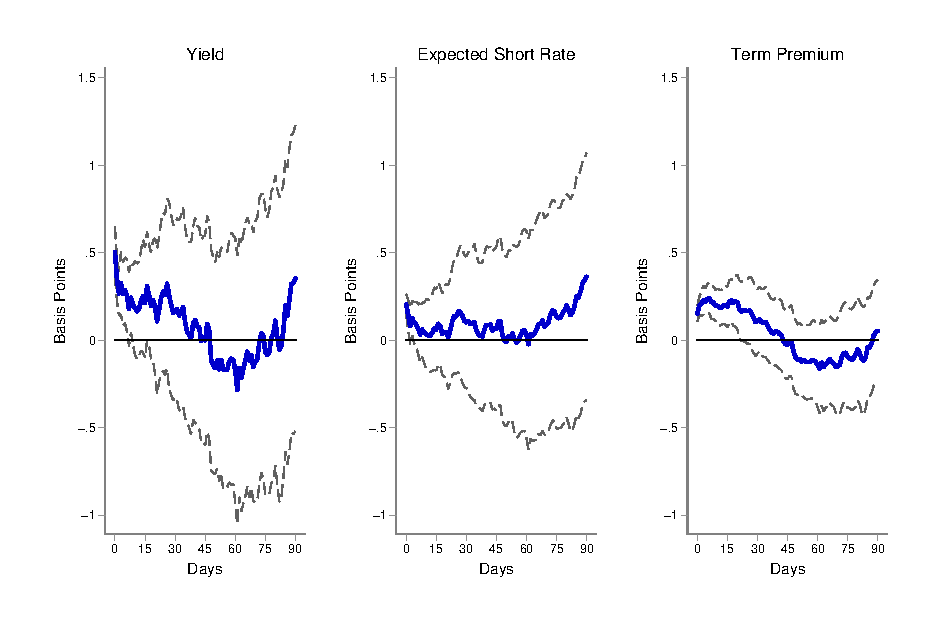
\includegraphics[trim={0cm 0cm 0cm 0cm},clip,height=0.24\textheight,width=\linewidth]{../Figures/LPs/LagDep-FX/Path/US/DCMP/PathUSDnomyptp24m.eps} \\
						\vspace{-0.35cm}
						\caption{Path Shock: 2000-2019} \label{subfig:LPUS2Ypath}
					\end{subfigure}
					
					\begin{subfigure}[t]{\linewidth}
						\includegraphics[trim={0cm 0cm 0cm 0cm},clip,height=0.24\textheight,width=\linewidth]{../Figures/LPs/LagDep-FX/LSAP/US/DCMP/LSAPUSDnomyptp24m.eps} \\
						\vspace{-0.35cm}
						\caption{LSAP Shock: 2009-2019} \label{subfig:LPUS2Ylsap}
					\end{subfigure}
				\end{center}
				\fignotes{This figure shows the response following \cite{Jorda:2005} of the 2-year U.S. yield and its components to U.S. monetary policy shocks. The U.S. yield is the zero coupon yield from \cite{GSW:2007}. The yield is decomposed into an expected future short-term interest rate and a term premium following \cite{KimWright:2005}. The target, path and LSAP shocks are identified using high-frequency data around Fed's monetary policy announcements, see section \ref{sec:USMPS} for details.}
			\end{minipage}
		\end{center}
	\end{figure}

	\pagebreak[4]
	
	\begin{figure}[tbph]
		\caption{Response of 10-Year U.S. Yield to U.S. Monetary Policy Shocks} \label{fig:LPUS10Y}
		\begin{center}
			\begin{minipage}{\linewidth}
				\begin{center}
					\begin{subfigure}[t]{\linewidth}
						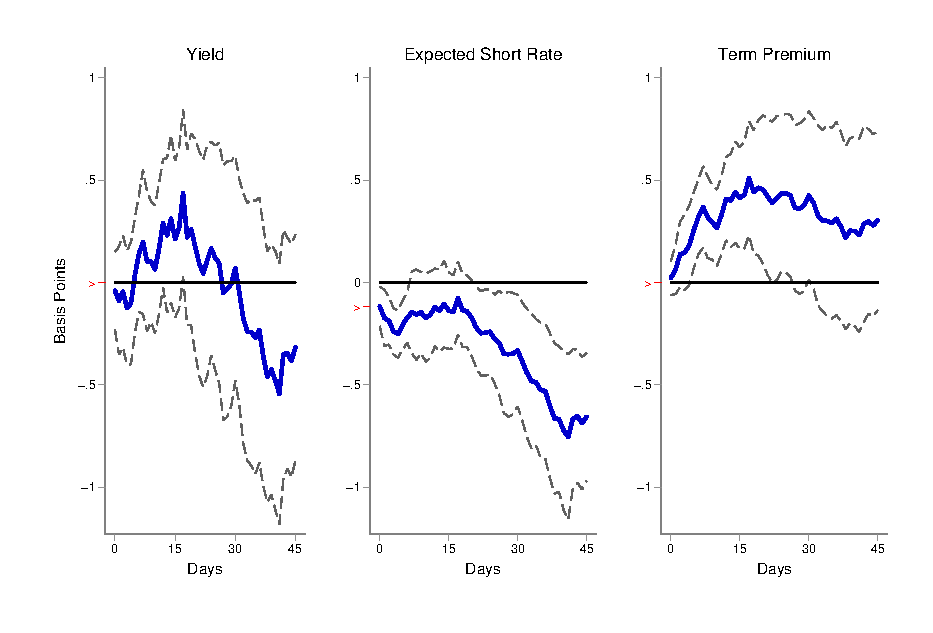
\includegraphics[trim={0cm 0cm 0cm 0cm},clip,height=0.24\textheight,width=\linewidth]{../Figures/LPs/LagDep-FX/Target/US/DCMP/TargetUSDnomyptp120m.eps} \\
						\vspace{-0.35cm}
						\caption{Target Shock: 2000-2008} \label{subfig:LPUS10Ytarget}
						\vspace{0.4cm}
					\end{subfigure}
					
					\begin{subfigure}[t]{\linewidth}
						\includegraphics[trim={0cm 0cm 0cm 0cm},clip,height=0.24\textheight,width=\linewidth]{../Figures/LPs/LagDep-FX/Path/US/DCMP/PathUSDnomyptp120m.eps} \\
						\vspace{-0.35cm}
						\caption{Path Shock: 2000-2019} \label{subfig:LPUS10Ypath}
					\end{subfigure}
					
					\begin{subfigure}[t]{\linewidth}
						\includegraphics[trim={0cm 0cm 0cm 0cm},clip,height=0.24\textheight,width=\linewidth]{../Figures/LPs/LagDep-FX/LSAP/US/DCMP/LSAPUSDnomyptp120m.eps} \\
						\vspace{-0.35cm}
						\caption{LSAP Shock: 2009-2019} \label{subfig:LPUS10Ylsap}
					\end{subfigure}
				\end{center}
				\fignotes{This figure shows the response following \cite{Jorda:2005} of the 10-year U.S. yield and its components to U.S. monetary policy shocks. The U.S. yield is the zero coupon yield from \cite{GSW:2007}. The yield is decomposed into an expected future short-term interest rate and a term premium following \cite{KimWright:2005}. The target, path and LSAP shocks are identified using high-frequency data around Fed's monetary policy announcements, see section \ref{sec:USMPS} for details.}
			\end{minipage}
		\end{center}
	\end{figure}
\end{document}
% trim = {<left> <lower> <right> <upper>}
%\documentclass{article}
\usepackage{graphicx}
\usepackage[margin=1in]{geometry}
\usepackage[outdir=./]{epstopdf}  					% Avoids errors when input figures
\usepackage[labelsep=period,labelfont=bf]{caption}
%\usepackage{subcaption}

\begin{document}
	\begin{figure}[tbph]
		\caption{Response of 2-Year Emerging Market Yield to U.S. Monetary Policy Shocks} \label{fig:LPEM2Y}
		\begin{center}
			\begin{minipage}{\linewidth}
				\begin{center}
					\begin{subfigure}[t]{\linewidth}
						\includegraphics[trim={0cm 0cm 0cm 0cm},clip,height=0.24\textheight,width=\linewidth]{../Figures/LPs/LagDep-FX/Target/EM/TargetEMnomyptpphi24m.eps} \\
						\vspace{-0.35cm}
						\caption{Target Shock: 2000-2008} \label{subfig:LPEM2Ytarget}
						\vspace{0.4cm}
					\end{subfigure}
					
					\begin{subfigure}[t]{\linewidth}
						\includegraphics[trim={0cm 0cm 0cm 0cm},clip,height=0.24\textheight,width=\linewidth]{../Figures/LPs/LagDep-FX/Path/EM/PathEMnomyptpphi24m.eps} \\
						\vspace{-0.35cm}
						\caption{Path Shock: 2000-2019} \label{subfig:LPEM2Ypath}
					\end{subfigure}
					
					\begin{subfigure}[t]{\linewidth}
						\includegraphics[trim={0cm 0cm 0cm 0cm},clip,height=0.24\textheight,width=\linewidth]{../Figures/LPs/LagDep-FX/LSAP/EM/LSAPEMnomyptpphi24m.eps} \\
						\vspace{-0.35cm}
						\caption{LSAP Shock: 2009-2019} \label{subfig:LPEM2Ylsap}
					\end{subfigure}
				\end{center}
				\fignotes{This figure shows the response following \cite{Jorda:2005} of the 2-year emerging market nominal yield and its components to U.S. monetary policy shocks. The nominal yield is decomposed into an expected future short-term interest rate (ER), a term premium (TP) and a credit risk premium (CRP). The target, path and LSAP shocks are identified using high-frequency data around Fed's monetary policy announcements, see section \ref{sec:USMPS} for details.}
			\end{minipage}
		\end{center}
	\end{figure}
	
	\pagebreak[4]
	
	\begin{figure}[tbph]
		\caption{Response of 10-Year Emerging Market Yield to U.S. Monetary Policy Shocks} \label{fig:LPEM10Y}
		\begin{center}
			\begin{minipage}{\linewidth}
				\begin{center}
					\begin{subfigure}[t]{\linewidth}
						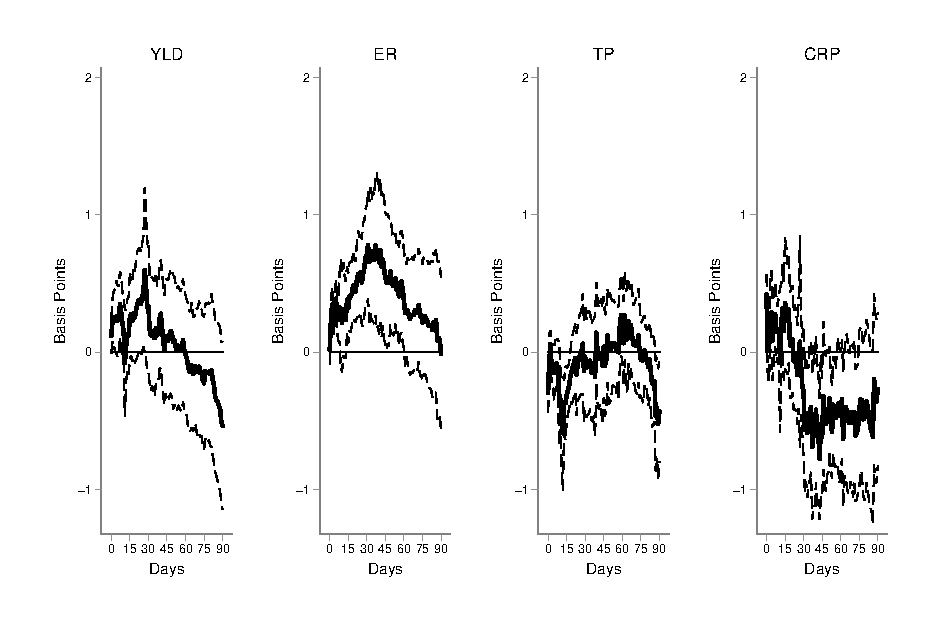
\includegraphics[trim={0cm 0cm 0cm 0cm},clip,height=0.24\textheight,width=\linewidth]{../Figures/LPs/LagDep-FX/Target/EM/TargetEMnomyptpphi120m.eps} \\
						\vspace{-0.35cm}
						\caption{Target Shock: 2000-2008} \label{subfig:LPEM10Ytarget}
						\vspace{0.4cm}
					\end{subfigure}
					
					\begin{subfigure}[t]{\linewidth}
						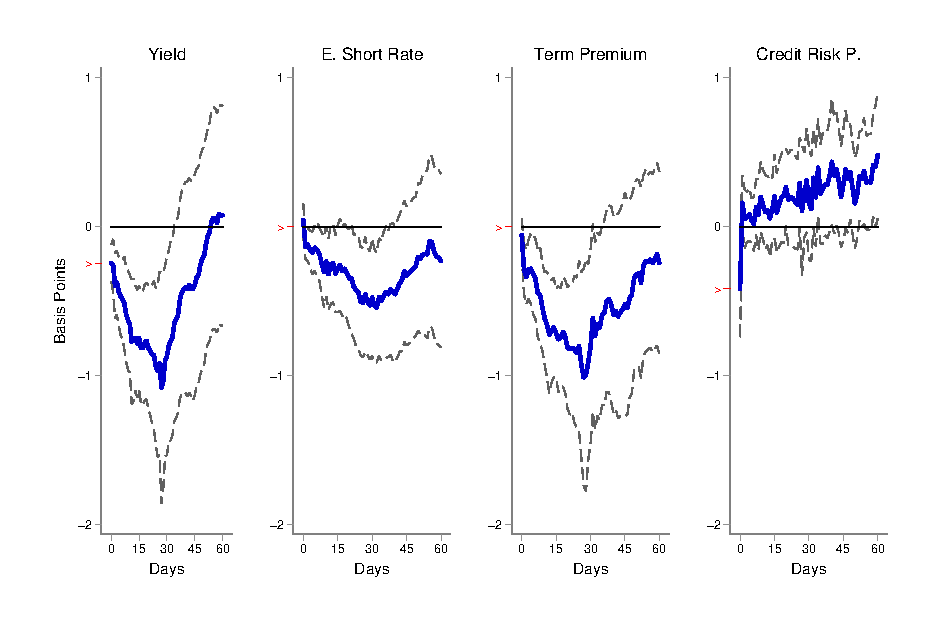
\includegraphics[trim={0cm 0cm 0cm 0cm},clip,height=0.24\textheight,width=\linewidth]{../Figures/LPs/LagDep-FX/Path/EM/PathEMnomyptpphi120m.eps} \\
						\vspace{-0.35cm}
						\caption{Path Shock: 2000-2019} \label{subfig:LPEM10Ypath}
					\end{subfigure}
					
					\begin{subfigure}[t]{\linewidth}
						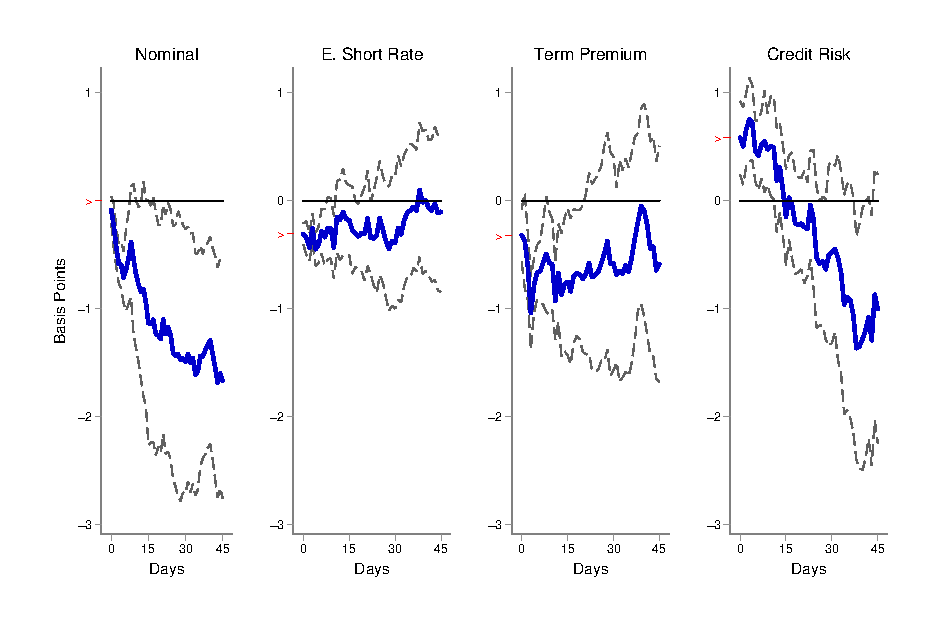
\includegraphics[trim={0cm 0cm 0cm 0cm},clip,height=0.24\textheight,width=\linewidth]{../Figures/LPs/LagDep-FX/LSAP/EM/LSAPEMnomyptpphi120m.eps} \\
						\vspace{-0.35cm}
						\caption{LSAP Shock: 2009-2019} \label{subfig:LPEM10Ylsap}
					\end{subfigure}
				\end{center}
				\fignotes{This figure shows the response following \cite{Jorda:2005} of the 10-year emerging market nominal yield and its components to U.S. monetary policy shocks. The nominal yield is decomposed into an expected future short-term interest rate (ER), a term premium (TP) and a credit risk premium (CRP). The target, path and LSAP shocks are identified using high-frequency data around Fed's monetary policy announcements, see section \ref{sec:USMPS} for details.}
			\end{minipage}
		\end{center}
	\end{figure}
\end{document}
% trim = {<left> <lower> <right> <upper>}
%\documentclass{article}
\usepackage{graphicx}
\usepackage[margin=1in]{geometry}
\usepackage[outdir=./]{epstopdf}  					% Avoids errors when input figures
\usepackage[labelsep=period,labelfont=bf]{caption}
%\usepackage{subcaption}

\begin{document}
	\begin{figure}[tbph]
		\caption{Response of the U.S. Yield Curve to a Target Surprise: 2000-2008} \label{fig:LPUStarget}
		\begin{center}
			\begin{minipage}{\linewidth}
				\begin{center}
					\begin{subfigure}[t]{\linewidth}
						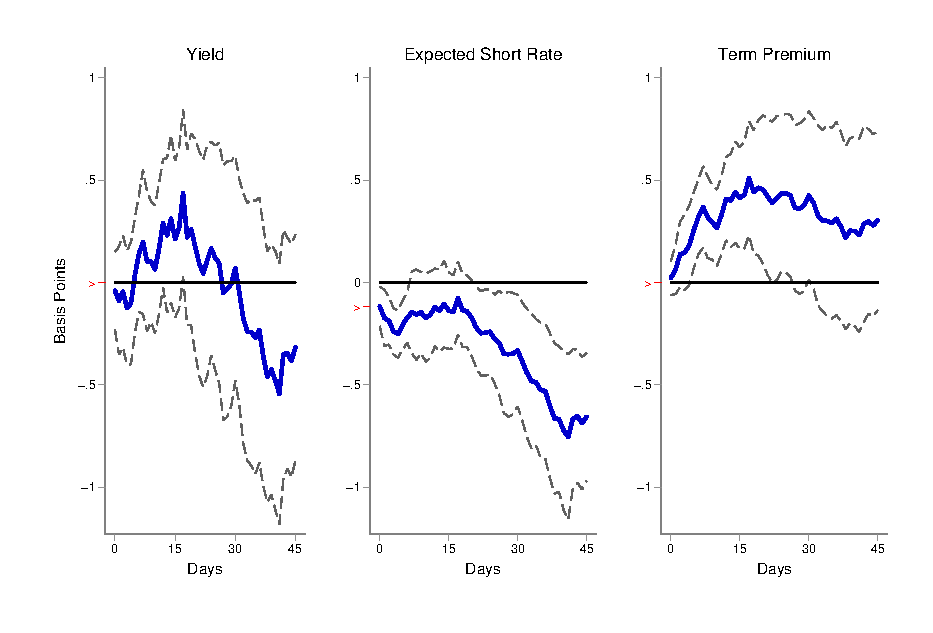
\includegraphics[trim={0cm 0cm 0cm 0cm},clip,height=0.35\textheight,width=\linewidth]{../Figures/LPs/LagDep-FX/Target/US/DCMP/TargetUSDnomyptp120m.eps} \\
						\vspace{-0.35cm}
						\caption{10-Year Yield} \label{subfig:LPUS10Ytarget}
						\vspace{0.4cm}
					\end{subfigure}
					
					\vspace{0.5cm}
					
					\begin{subfigure}[t]{\linewidth}
						\includegraphics[trim={0cm 0cm 0cm 0cm},clip,height=0.35\textheight,width=\linewidth]{../Figures/LPs/LagDep-FX/Target/US/DCMP/TargetUSDnomyptp24m.eps} \\
						\vspace{-0.35cm}
						\caption{2-Year Yield} \label{subfig:LPUS2Ytarget}
						\vspace{0.4cm}
					\end{subfigure}
				\end{center}
				\fignotes{This figure shows the response following \cite{Jorda:2005} of the 10- and 2-year U.S. yields and their components to a target surprise. The U.S. yield is the zero coupon yield from \cite{GSW:2007}. The yield is decomposed into an expected future short-term interest rate and a term premium following \cite{KimWright:2005}. Target surprises are identified using high-frequency data around Fed's monetary policy announcements, see section \ref{sec:USMPS} for details.}
			\end{minipage}
		\end{center}
	\end{figure}

	\pagebreak[4]
	
	\begin{figure}[tbph]
		\caption{Response of the U.S. Yield Curve to a Forward Guidance Surprise: 2000-2019} \label{fig:LPUSpath}
		\begin{center}
			\begin{minipage}{\linewidth}
				\begin{center}
					\begin{subfigure}[t]{\linewidth}
						\includegraphics[trim={0cm 0cm 0cm 0cm},clip,height=0.35\textheight,width=\linewidth]{../Figures/LPs/LagDep-FX/Path/US/DCMP/PathUSDnomyptp120m.eps} \\
						\vspace{-0.35cm}
						\caption{10-Year Yield} \label{subfig:LPUS10Ypath}
					\end{subfigure}
					
					\vspace{0.5cm}
					
					\begin{subfigure}[t]{\linewidth}
						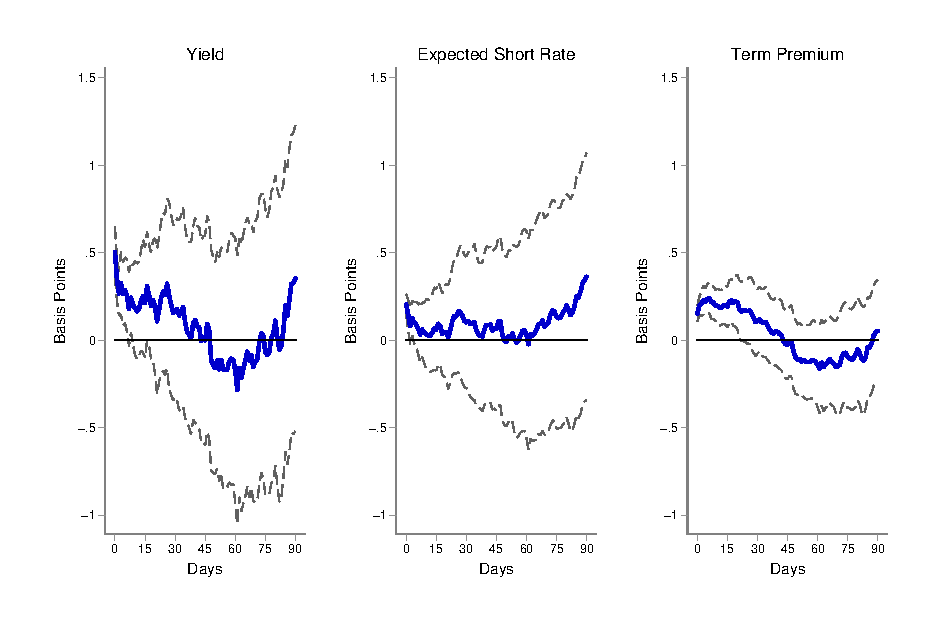
\includegraphics[trim={0cm 0cm 0cm 0cm},clip,height=0.35\textheight,width=\linewidth]{../Figures/LPs/LagDep-FX/Path/US/DCMP/PathUSDnomyptp24m.eps} \\
						\vspace{-0.35cm}
						\caption{2-Year Yield} \label{subfig:LPUS2Ypath}
					\end{subfigure}
				\end{center}
				\fignotes{This figure shows the response following \cite{Jorda:2005} of the 10- and 2-year U.S. yields and their components to a forward guidance surprise. The U.S. yield is the zero coupon yield from \cite{GSW:2007}. The yield is decomposed into an expected future short-term interest rate and a term premium following \cite{KimWright:2005}. Forward guidance surprises are identified using high-frequency data around Fed's monetary policy announcements, see section \ref{sec:USMPS} for details.}
			\end{minipage}
		\end{center}
	\end{figure}

	\pagebreak[4]
	
	\begin{figure}[tbph]
		\caption{Response of the U.S. Yield Curve to an Asset Purchase Surprise: 2009-2019} \label{fig:LPUSlsap}
		\begin{center}
			\begin{minipage}{\linewidth}
				\begin{center}
					\begin{subfigure}[t]{\linewidth}
						\includegraphics[trim={0cm 0cm 0cm 0cm},clip,height=0.35\textheight,width=\linewidth]{../Figures/LPs/LagDep-FX/LSAP/US/DCMP/LSAPUSDnomyptp120m.eps} \\
						\vspace{-0.35cm}
						\caption{10-Year Yield} \label{subfig:LPUS10Ylsap}
					\end{subfigure}
					
					\vspace{0.5cm}
					
					\begin{subfigure}[t]{\linewidth}
						\includegraphics[trim={0cm 0cm 0cm 0cm},clip,height=0.35\textheight,width=\linewidth]{../Figures/LPs/LagDep-FX/LSAP/US/DCMP/LSAPUSDnomyptp24m.eps} \\
						\vspace{-0.35cm}
						\caption{2-Year Yield} \label{subfig:LPUS2Ylsap}
					\end{subfigure}
				\end{center}
				\fignotes{This figure shows the response following \cite{Jorda:2005} of the 10- and 2-year U.S. yields and their components to an asset purchase surprise. The U.S. yield is the zero coupon yield from \cite{GSW:2007}. The yield is decomposed into an expected future short-term interest rate and a term premium following \cite{KimWright:2005}. Asset purchase surprises are identified using high-frequency data around Fed's monetary policy announcements, see section \ref{sec:USMPS} for details.}
			\end{minipage}
		\end{center}
	\end{figure}
\end{document}
% trim = {<left> <lower> <right> <upper>} % appendix
\documentclass{article}
\usepackage[margin=1in]{geometry}
\usepackage[outdir=./]{epstopdf}  					% Avoids errors when input figures
\usepackage[labelsep=period,labelfont=bf]{caption}
%\usepackage{subcaption}
\usepackage{graphicx}
%\graphicspath{{../Figures/LPs/LagDep-FX/Target/EM/}{../Figures/LPs/LagDep-FX/Path/EM/}{../Figures/LPs/LagDep-FX/LSAP/EM/}}

\begin{document}
	\begin{figure}[tbph]
		\caption{Response of the EM Yield Curve to a Target Surprise: 2000-2008} \label{fig:LPEMtarget}
		\begin{center}
			\begin{minipage}{\linewidth}
				\begin{center}
					\begin{subfigure}[t]{\linewidth}
						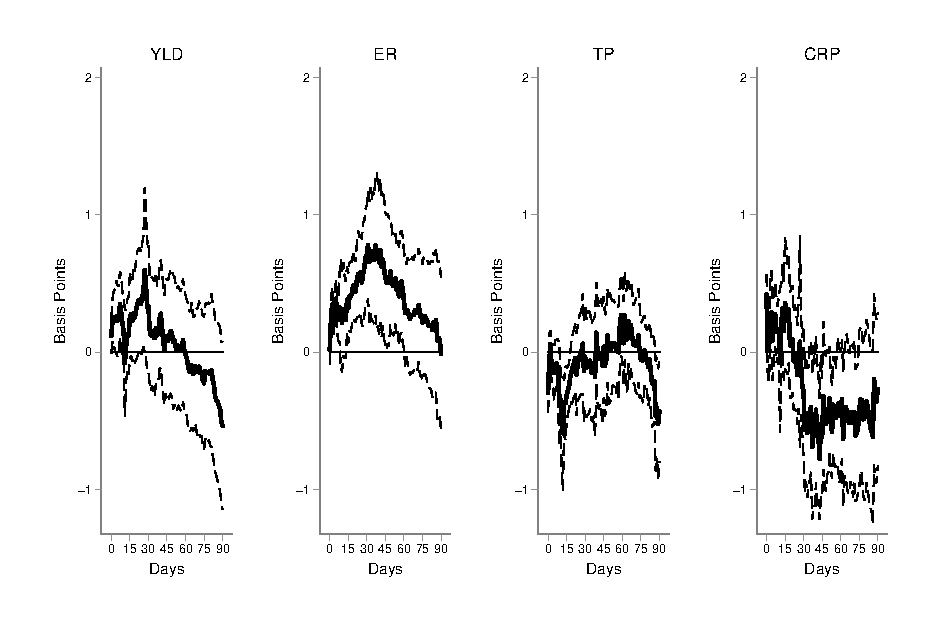
\includegraphics[trim={0cm 0cm 0cm 0cm},clip,height=0.35\textheight,width=\linewidth]{../Figures/LPs/LagDep-FX/Target/EM/TargetEMnomyptpphi120m.eps} \\
						\vspace{-0.35cm}
						\caption{10-Year Yield} \label{subfig:LPEM10Ytarget}
						\vspace{0.4cm}
					\end{subfigure}
				
					\vspace{0.5cm}
					
					\begin{subfigure}[t]{\linewidth}
						\includegraphics[trim={0cm 0cm 0cm 0cm},clip,height=0.35\textheight,width=\linewidth]{../Figures/LPs/LagDep-FX/Target/EM/TargetEMnomyptpphi24m.eps} \\
						\vspace{-0.35cm}
						\caption{2-Year Yield} \label{subfig:LPEM2Ytarget}
						\vspace{0.4cm}
					\end{subfigure}
				\end{center}
				\fignotes{This figure shows the response following \cite{Jorda:2005} of the 10- and 2-year emerging market (EM) nominal yields and their components to a target surprise. Nominal yields are decomposed into an expected future short-term interest rate, a term premium and a credit risk compensation, see section \ref{sec:Decomposition} for details. Target surprises are identified using high-frequency data around Fed's monetary policy announcements, see section \ref{sec:USMPS} for details.}
			\end{minipage}
		\end{center}
	\end{figure}
	
	\pagebreak[4]
	
	\begin{figure}[tbph]
		\caption{Response of the EM Yield Curve to a Forward Guidance Surprise: 2000-2019} \label{fig:LPEMpath}
		\begin{center}
			\begin{minipage}{\linewidth}
				\begin{center}
					\begin{subfigure}[t]{\linewidth}
						\includegraphics[trim={0cm 0cm 0cm 0cm},clip,height=0.35\textheight,width=\linewidth]{../Figures/LPs/LagDep-FX/Path/EM/PathEMnomyptpphi120m.eps} \\
						\vspace{-0.35cm}
						\caption{10-Year Yield} \label{subfig:LPEM10Ypath}
					\end{subfigure}
					
					\vspace{0.5cm}
					
					\begin{subfigure}[t]{\linewidth}
						\includegraphics[trim={0cm 0cm 0cm 0cm},clip,height=0.35\textheight,width=\linewidth]{../Figures/LPs/LagDep-FX/Path/EM/PathEMnomyptpphi24m.eps} \\
						\vspace{-0.35cm}
						\caption{2-Year Yield} \label{subfig:LPEM2Ypath}
					\end{subfigure}
				\end{center}
				\fignotes{This figure shows the response following \cite{Jorda:2005} of the 10- and 2-year emerging market (EM) nominal yields and their components to a forward guidance surprise. Nominal yields are decomposed into an expected future short-term interest rate, a term premium and a credit risk compensation, see section \ref{sec:Decomposition} for details. Forward guidance surprises are identified using high-frequency data around Fed's monetary policy announcements, see section \ref{sec:USMPS} for details.}
			\end{minipage}
		\end{center}
	\end{figure}
	
	\pagebreak[4]
	
	\begin{figure}[tbph]
		\caption{Response of the EM Yield Curve to an Asset Purchase Surprise: 2009-2019} \label{fig:LPEMlsap}
		\begin{center}
			\begin{minipage}{\linewidth}
				\begin{center}
					\begin{subfigure}[t]{\linewidth}
						\includegraphics[trim={0cm 0cm 0cm 0cm},clip,height=0.35\textheight,width=\linewidth]{../Figures/LPs/LagDep-FX/LSAP/EM/LSAPEMnomyptpphi120m.eps} \\
						\vspace{-0.35cm}
						\caption{10-Year Yield} \label{subfig:LPEM10Ylsap}
					\end{subfigure}
					
					\vspace{0.5cm}
					
					\begin{subfigure}[t]{\linewidth}
						\includegraphics[trim={0cm 0cm 0cm 0cm},clip,height=0.35\textheight,width=\linewidth]{../Figures/LPs/LagDep-FX/LSAP/EM/LSAPEMnomyptpphi24m.eps} \\
						\vspace{-0.35cm}
						\caption{2-Year Yield} \label{subfig:LPEM2Ylsap}
					\end{subfigure}
				\end{center}
				\fignotes{This figure shows the response following \cite{Jorda:2005} of the 10- and 2-year emerging market (EM) nominal yields and their components to an asset purchase. Nominal yields are decomposed into an expected future short-term interest rate, a term premium and a credit risk compensation, see section \ref{sec:Decomposition} for details. Asset purchase surprises are identified using high-frequency data around Fed's monetary policy announcements, see section \ref{sec:USMPS} for details.}
			\end{minipage}
		\end{center}
	\end{figure}
\end{document}
% trim = {<left> <lower> <right> <upper>}
%\documentclass{article}
\usepackage{graphicx}
\usepackage[margin=1in]{geometry}
\usepackage[outdir=./]{epstopdf}  					% Avoids errors when input figures
\usepackage[labelsep=period,labelfont=bf]{caption}
%\usepackage{subcaption}

\begin{document}
	\begin{figure}[tbph]
		\caption{Response of 2-Year Advanced Country Yield to U.S. Monetary Policy Surprises} \label{fig:LPAE2Y}
		\begin{center}
			\begin{minipage}{\linewidth}
				\begin{center}
					\begin{subfigure}[t]{\linewidth}
						\includegraphics[trim={0cm 0cm 0cm 0cm},clip,height=0.24\textheight,width=\linewidth]{../Figures/LPs/LagDep-FX/Target/AE/TargetAEnomyptpphi24m.eps} \\
						\vspace{-0.35cm}
						\caption{Target Surprise: 2000-2008} \label{subfig:LPAE2Ytarget}
						\vspace{0.4cm}
					\end{subfigure}
					
					\begin{subfigure}[t]{\linewidth}
						\includegraphics[trim={0cm 0cm 0cm 0cm},clip,height=0.24\textheight,width=\linewidth]{../Figures/LPs/LagDep-FX/Path/AE/PathAEnomyptpphi24m.eps} \\
						\vspace{-0.35cm}
						\caption{Forward Guidance Surprise: 2000-2019} \label{subfig:LPAE2Ypath}
					\end{subfigure}
					
					\begin{subfigure}[t]{\linewidth}
						\includegraphics[trim={0cm 0cm 0cm 0cm},clip,height=0.24\textheight,width=\linewidth]{../Figures/LPs/LagDep-FX/LSAP/AE/LSAPAEnomyptpphi24m.eps} \\
						\vspace{-0.35cm}
						\caption{Asset Purchase Surprise: 2009-2019} \label{subfig:LPAE2Ylsap}
					\end{subfigure}
				\end{center}
				\fignotes{This figure shows the response following \cite{Jorda:2005} of the 2-year advanced country nominal yield and its components to U.S. monetary policy surprises. The nominal yield is decomposed into an expected future short-term interest rate (ER) and a term premium (TP). The target, forward guidance and asset purchase surprises are identified using high-frequency data around Fed's monetary policy announcements, see section \ref{sec:USMPS} for details.}
			\end{minipage}
		\end{center}
	\end{figure}
	
	\pagebreak[4]
	
	\begin{figure}[tbph]
		\caption{Response of 10-Year Advanced Country Yield to U.S. Monetary Policy Surprises} \label{fig:LPAE10Y}
		\begin{center}
			\begin{minipage}{\linewidth}
				\begin{center}
					\begin{subfigure}[t]{\linewidth}
						\includegraphics[trim={0cm 0cm 0cm 0cm},clip,height=0.24\textheight,width=\linewidth]{../Figures/LPs/LagDep-FX/Target/AE/TargetAEnomyptpphi120m.eps} \\
						\vspace{-0.35cm}
						\caption{Target Surprise: 2000-2008} \label{subfig:LPAE10Ytarget}
						\vspace{0.4cm}
					\end{subfigure}
					
					\begin{subfigure}[t]{\linewidth}
						\includegraphics[trim={0cm 0cm 0cm 0cm},clip,height=0.24\textheight,width=\linewidth]{../Figures/LPs/LagDep-FX/Path/AE/PathAEnomyptpphi120m.eps} \\
						\vspace{-0.35cm}
						\caption{Forward Guidance Surprise: 2000-2019} \label{subfig:LPAE10Ypath}
					\end{subfigure}
					
					\begin{subfigure}[t]{\linewidth}
						\includegraphics[trim={0cm 0cm 0cm 0cm},clip,height=0.24\textheight,width=\linewidth]{../Figures/LPs/LagDep-FX/LSAP/AE/LSAPAEnomyptpphi120m.eps} \\
						\vspace{-0.35cm}
						\caption{Asset Purchase Surprise: 2009-2019} \label{subfig:LPAE10Ylsap}
					\end{subfigure}
				\end{center}
				\fignotes{This figure shows the response following \cite{Jorda:2005} of the 10-year advanced country nominal yield and its components to U.S. monetary policy surprises. The nominal yield is decomposed into an expected future short-term interest rate (ER) and a term premium (TP). The target, forward guidance and asset purchase surprises are identified using high-frequency data around Fed's monetary policy announcements, see section \ref{sec:USMPS} for details.}
			\end{minipage}
		\end{center}
	\end{figure}
\end{document}
% trim = {<left> <lower> <right> <upper>}
%\documentclass{article}
\usepackage{graphicx}
\usepackage[margin=1in]{geometry}
\usepackage[outdir=./]{epstopdf}  					% Avoids errors when input figures
\usepackage[labelsep=period,labelfont=bf]{caption}
%\usepackage{subcaption}

\begin{document}

% trim = {<left> <lower> <right> <upper>}

\begin{figure}[tbph]
	\caption{Response of the Forward Premium to U.S. Monetary Policy Shocks: EM}
	\label{fig:LPEMRHO}
	\begin{subfigure}[t]{\textwidth}
		\begin{center}
			\includegraphics[trim={0cm 0cm 0cm 0cm},clip,height=0.26\textheight,width=1\textwidth]{../Figures/LPs/LagDep-FX/Target/EM/TargetEMrho.eps} \\
			\caption{Target Shock: 2000-2008} \label{subfig:LPEMRHOtarget}
%			\vspace{.5cm}
		\end{center}
	\end{subfigure}
	
	\begin{subfigure}[t]{\textwidth}
		\begin{center}
			\includegraphics[trim={0cm 0cm 0cm 0cm},clip,height=0.26\textheight,width=1\textwidth]{../Figures/LPs/LagDep-FX/Path/EM/PathEMrho.eps} \\
			\caption{Path Shock: 2000-2019} \label{subfig:LPEMRHOpath}
%			\vspace{.4cm}
		\end{center}
	\end{subfigure}
	
	\begin{subfigure}[t]{\textwidth}
		\begin{center}
			\includegraphics[trim={0cm 0cm 0cm 0cm},clip,height=0.26\textheight,width=1\textwidth]{../Figures/LPs/LagDep-FX/LSAP/EM/LSAPEMrho.eps} \\
			\caption{LSAP Shock: 2009-2019} \label{subfig:LPEMRHOlsap}
			%			\vspace{.4cm}
		\end{center}
	\end{subfigure}

%	\vspace{-0.4cm} \caption*{\footnotesize{\textit{Notes}: Notes.}}
\end{figure}

\pagebreak[4]

\begin{figure}[tbph]
	\caption{Response of the Forward Premium to U.S. Monetary Policy Shocks: AE}
	\label{fig:LPAERHO}
	\begin{subfigure}[t]{\textwidth}
		\begin{center}
			\includegraphics[trim={0cm 0cm 0cm 0cm},clip,height=0.26\textheight,width=1\textwidth]{../Figures/LPs/LagDep-FX/Target/AE/TargetAErho.eps} \\
			\caption{Target Shock: 2000-2008} \label{subfig:LPAERHOtarget}
			%			\vspace{.5cm}
		\end{center}
	\end{subfigure}
	
	\begin{subfigure}[t]{\textwidth}
		\begin{center}
			\includegraphics[trim={0cm 0cm 0cm 0cm},clip,height=0.26\textheight,width=1\textwidth]{../Figures/LPs/LagDep-FX/Path/AE/PathAErho.eps} \\
			\caption{Path Shock: 2000-2019} \label{subfig:LPAERHOpath}
			%			\vspace{.4cm}
		\end{center}
	\end{subfigure}
	
	\begin{subfigure}[t]{\textwidth}
		\begin{center}
			\includegraphics[trim={0cm 0cm 0cm 0cm},clip,height=0.26\textheight,width=1\textwidth]{../Figures/LPs/LagDep-FX/LSAP/AE/LSAPAErho.eps} \\
			\caption{LSAP Shock: 2009-2019} \label{subfig:LPAERHOlsap}
			%			\vspace{.4cm}
		\end{center}
	\end{subfigure}
	
	%	\vspace{-0.4cm} \caption*{\footnotesize{\textit{Notes}: Notes.}}
\end{figure}

\end{document}
 % appendix
%\documentclass{article}
\usepackage{graphicx}
\usepackage[margin=1in]{geometry}
\usepackage[outdir=./]{epstopdf}  					% Avoids errors when input figures
\usepackage[labelsep=period,labelfont=bf]{caption}
%\usepackage{subcaption}

\begin{document}
	\begin{figure}[tbph]
		\caption{Response of the Forward Premium to U.S. Monetary Policy Surprises: AE} \label{fig:LPAERHO}
		\begin{center}
			\begin{minipage}{\linewidth}
				\begin{center}
					\begin{subfigure}[t]{\linewidth}
						\includegraphics[trim={0cm 0cm 0cm 0cm},clip,height=0.24\textheight,width=\linewidth]{../Figures/LPs/LagDep-FX/Target/AE/TargetAErho.eps} \\
						\vspace{-0.35cm}
						\caption{Target Surprise: 2000-2008} \label{subfig:LPAERHOtarget}
						\vspace{0.4cm}
					\end{subfigure}
					
					\begin{subfigure}[t]{\linewidth}
						\includegraphics[trim={0cm 0cm 0cm 0cm},clip,height=0.24\textheight,width=\linewidth]{../Figures/LPs/LagDep-FX/Path/AE/PathAErho.eps} \\
						\vspace{-0.35cm}
						\caption{Forward Guidance Surprise: 2000-2019} \label{subfig:LPAERHOpath}
					\end{subfigure}
					
					\begin{subfigure}[t]{\linewidth}
						\includegraphics[trim={0cm 0cm 0cm 0cm},clip,height=0.24\textheight,width=\linewidth]{../Figures/LPs/LagDep-FX/LSAP/AE/LSAPAErho.eps} \\
						\vspace{-0.35cm}
						\caption{Asset Purchase Surprise: 2009-2019} \label{subfig:LPAERHOlsap}
					\end{subfigure}
				\end{center}
				\fignotes{This figure shows the response following \cite{Jorda:2005} of the 2- and 10-year forward premium for advanced countries (AE) to U.S. monetary policy surprises. The forward premium is calculated using cross-currency swaps, which are in turn constructed using cross-currency basis swaps and interest rate swaps, see section \ref{sec:YCsynt} for details. The target, forward guidance and asset purchase surprises are identified using high-frequency data around Fed's monetary policy announcements, see section \ref{sec:USMPS} for details. The 90\% confidence bands are based on Driscoll--Kraay standard errors.}
			\end{minipage}
		\end{center}
	\end{figure}
\end{document}
% trim = {<left> <lower> <right> <upper>}

\begin{landscape}
	\newpage
\end{landscape}